\documentclass[twoside]{book}

% Packages required by doxygen
\usepackage{calc}
\usepackage{doxygen}
\usepackage{graphicx}
\usepackage[utf8]{inputenc}
\usepackage{makeidx}
\usepackage{multicol}
\usepackage{multirow}
\usepackage{textcomp}
\usepackage[table]{xcolor}

% Font selection
\usepackage[T1]{fontenc}
\usepackage{mathptmx}
\usepackage[scaled=.90]{helvet}
\usepackage{courier}
\usepackage{amssymb}
\usepackage{sectsty}
\renewcommand{\familydefault}{\sfdefault}
\allsectionsfont{%
  \fontseries{bc}\selectfont%
  \color{darkgray}%
}
\renewcommand{\DoxyLabelFont}{%
  \fontseries{bc}\selectfont%
  \color{darkgray}%
}

% Page & text layout
\usepackage{geometry}
\geometry{%
  a4paper,%
  top=2.5cm,%
  bottom=2.5cm,%
  left=2.5cm,%
  right=2.5cm%
}
\tolerance=750
\hfuzz=15pt
\hbadness=750
\setlength{\emergencystretch}{15pt}
\setlength{\parindent}{0cm}
\setlength{\parskip}{0.2cm}
\makeatletter
\renewcommand{\paragraph}{%
  \@startsection{paragraph}{4}{0ex}{-1.0ex}{1.0ex}{%
    \normalfont\normalsize\bfseries\SS@parafont%
  }%
}
\renewcommand{\subparagraph}{%
  \@startsection{subparagraph}{5}{0ex}{-1.0ex}{1.0ex}{%
    \normalfont\normalsize\bfseries\SS@subparafont%
  }%
}
\makeatother

% Headers & footers
\usepackage{fancyhdr}
\pagestyle{fancyplain}
\fancyhead[LE]{\fancyplain{}{\bfseries\thepage}}
\fancyhead[CE]{\fancyplain{}{}}
\fancyhead[RE]{\fancyplain{}{\bfseries\leftmark}}
\fancyhead[LO]{\fancyplain{}{\bfseries\rightmark}}
\fancyhead[CO]{\fancyplain{}{}}
\fancyhead[RO]{\fancyplain{}{\bfseries\thepage}}
\fancyfoot[LE]{\fancyplain{}{}}
\fancyfoot[CE]{\fancyplain{}{}}
\fancyfoot[RE]{\fancyplain{}{\bfseries\scriptsize Generated on Wed Nov 22 2023 15\-:27\-:36 for C\-A\-L\-I\-C\-E\-A\-N\-A\-L\-Y\-S\-I\-S by Doxygen }}
\fancyfoot[LO]{\fancyplain{}{\bfseries\scriptsize Generated on Wed Nov 22 2023 15\-:27\-:36 for C\-A\-L\-I\-C\-E\-A\-N\-A\-L\-Y\-S\-I\-S by Doxygen }}
\fancyfoot[CO]{\fancyplain{}{}}
\fancyfoot[RO]{\fancyplain{}{}}
\renewcommand{\footrulewidth}{0.4pt}
\renewcommand{\chaptermark}[1]{%
  \markboth{#1}{}%
}
\renewcommand{\sectionmark}[1]{%
  \markright{\thesection\ #1}%
}

% Indices & bibliography
\usepackage{natbib}
\usepackage[titles]{tocloft}
\setcounter{tocdepth}{3}
\setcounter{secnumdepth}{5}
\makeindex

% Custom commands
\newcommand{\clearemptydoublepage}{%
  \newpage{\pagestyle{empty}\cleardoublepage}%
}


%===== C O N T E N T S =====

\begin{document}

% Titlepage & ToC
\pagenumbering{roman}
\begin{titlepage}
\vspace*{7cm}
\begin{center}%
{\Large C\-A\-L\-I\-C\-E\-A\-N\-A\-L\-Y\-S\-I\-S \\[1ex]\large 1.\-3.\-5 }\\
\vspace*{1cm}
{\large Generated by Doxygen 1.8.5}\\
\vspace*{0.5cm}
{\small Wed Nov 22 2023 15:27:36}\\
\end{center}
\end{titlepage}
\clearemptydoublepage
\tableofcontents
\clearemptydoublepage
\pagenumbering{arabic}

%--- Begin generated contents ---
\chapter{Todo List}
\label{todo}

\begin{DoxyRefList}
\item[\label{todo__todo000001}%
Class \doxyref{C\-A\-L\-I\-C\-E\-:\-:Acquisition\-Data}{p.}{classCALICE_1_1AcquisitionData} ]should we make a regular userlib class out of it?  
\item[\label{todo__todo000002}%
Class \doxyref{C\-A\-L\-I\-C\-E\-:\-:Beam\-Momentum}{p.}{classCALICE_1_1BeamMomentum} ]implement a constructor for F\-N\-A\-L slow readout data 
\item[\label{todo__todo000003}%
Class \doxyref{C\-A\-L\-I\-C\-E\-:\-:Beam\-Parameter}{p.}{classCALICE_1_1BeamParameter} ]\{Should this class be split into two? One for the beam and one for the detector parameters? Should the nominal and measured values be stored in separate folders?\}  
\item[\label{todo__todo000005}%
Global \doxyref{C\-A\-L\-I\-C\-E\-:\-:Daq\-Type\-Data\-Block\-:\-:finalize}{p.}{classCALICE_1_1DaqTypeDataBlock_a5aac4e6f4aef380287394ad36b30a40d} ()]can the algorithms in this method be templated?  
\item[\label{todo__todo000004}%
Global \doxyref{C\-A\-L\-I\-C\-E\-:\-:Daq\-Type\-Data\-Block\-:\-:get\-Int\-Arrays}{p.}{classCALICE_1_1DaqTypeDataBlock_aed8a8e75c1ca2befbf3f4c1bfe54e0a9} ()]\-: Should these methods really be public or only accessible by friend functions or ...? 

\-: Do we have to check whether they has been filled or not before we hand it to the user?  
\item[\label{todo__todo000006}%
Class \doxyref{C\-A\-L\-I\-C\-E\-:\-:Detector\-Transformation}{p.}{classCALICE_1_1DetectorTransformation} ]\{Should this class be split into two? One for the beam and one for the detector parameters? Should the nominal and measured values be stored in separate folders?\}  
\item[\label{todo__todo000007}%
Class \doxyref{C\-A\-L\-I\-C\-E\-:\-:Dhc\-Readout\-Conf\-Block}{p.}{classCALICE_1_1DhcReadoutConfBlock} ]Attention we may introduce a platform dependency here!!!! The structure of the object assumes that L\-C\-Generic\-Objects are aligned on 32 bits Need maybe revision for assumptions on data alignment, could be added as collection parameters,  
\item[\label{todo__todo000008}%
Class \doxyref{C\-A\-L\-I\-C\-E\-:\-:Experimental\-Setup}{p.}{classCALICE_1_1ExperimentalSetup} ]\{Should this class be split into two? One for the beam and one for the detector parameters? Should the nominal and measured values be stored in separate folders?\}  
\item[\label{todo__todo000014}%
Global \doxyref{C\-A\-L\-I\-C\-E\-:\-:Fe\-Info\-:\-:get\-Be\-Status}{p.}{classCALICE_1_1FeInfo_a56f6bb4e32c6016da0cedbbc86050c1a} () const ]needs better explanation.  
\item[\label{todo__todo000012}%
Global \doxyref{C\-A\-L\-I\-C\-E\-:\-:Fe\-Info\-:\-:get\-Fe\-Length}{p.}{classCALICE_1_1FeInfo_a8670ba7cf2806521398a0ad5b3081889} () const ]needs better explanation.  
\item[\label{todo__todo000010}%
Global \doxyref{C\-A\-L\-I\-C\-E\-:\-:Fe\-Info\-:\-:get\-Label}{p.}{classCALICE_1_1FeInfo_a67dd0f689121876bcae54f69813c29dd} () const ]needs better explanation.  
\item[\label{todo__todo000013}%
Global \doxyref{C\-A\-L\-I\-C\-E\-:\-:Fe\-Info\-:\-:set\-Be\-Status}{p.}{classCALICE_1_1FeInfo_a04552f8e75412662946c7b3c65dad0c5} (int be\-\_\-status)]needs better explanation.  
\item[\label{todo__todo000011}%
Global \doxyref{C\-A\-L\-I\-C\-E\-:\-:Fe\-Info\-:\-:set\-Fe\-Length}{p.}{classCALICE_1_1FeInfo_a884328110730cf0cb15c96aed00d3930} (int fe\-\_\-length)]needs better explanation.  
\item[\label{todo__todo000009}%
Global \doxyref{C\-A\-L\-I\-C\-E\-:\-:Fe\-Info\-:\-:set\-Label}{p.}{classCALICE_1_1FeInfo_a30d1e319c5b493268ee8f8674a9f0f6c} (int label)]needs better explanation.  
\item[\label{todo__todo000015}%
Global \doxyref{C\-A\-L\-I\-C\-E\-:\-:Mapping\-And\-Alignment\-:\-:get\-Cell\-Index}{p.}{classCALICE_1_1MappingAndAlignment_ab51a0f33e8d02234ddc96a399a02e9be} (U\-Int\-\_\-t module\-\_\-index, U\-Int\-\_\-t multiplex\-\_\-position, U\-Int\-\_\-t line\-\_\-i) const ]need more robust method to determine the number of lines per modules  
\item[\label{todo__todo000016}%
Global \doxyref{C\-A\-L\-I\-C\-E\-:\-:Mapping\-And\-Alignment\-:\-:get\-Module\-Index\-From\-Cell\-Index}{p.}{classCALICE_1_1MappingAndAlignment_a7c80e28c748f3238cf2edca2a8190dc3} (U\-Int\-\_\-t)]Extend function to handle situation in which a layer k does not exist in data but is simulated  
\item[\label{todo__todo000018}%
Global \doxyref{C\-A\-L\-I\-C\-E\-:\-:Module\-Connection\-:\-:get\-Module\-Type}{p.}{classCALICE_1_1ModuleConnection_a0330ce4dd3f58a935030dc1ffd715730} () const ]remove this redundant information?  
\item[\label{todo__todo000017}%
Global \doxyref{C\-A\-L\-I\-C\-E\-:\-:Module\-Connection\-:\-:set\-Module\-Type}{p.}{classCALICE_1_1ModuleConnection_a7c8661d2a87294ad724d63fc0c25d51d} (unsigned char type)]remove this redundant information?  
\item[\label{todo__todo000020}%
Global \doxyref{C\-A\-L\-I\-C\-E\-:\-:Module\-Description\-:\-:get\-Geometrical\-Cell\-Index}{p.}{classCALICE_1_1ModuleDescription_a51c9bc14fff2390f99a73e154c4c4e11} (U\-Int\-\_\-t cell\-\_\-index) const ]I did not find a more clever way than putting this index into the database.  
\item[\label{todo__todo000019}%
Global \doxyref{C\-A\-L\-I\-C\-E\-:\-:Module\-Description\-:\-:set\-Geometrical\-Cell\-Index}{p.}{classCALICE_1_1ModuleDescription_a3e14b75a948febdb14e7e5f394609c59} (U\-Int\-\_\-t cell\-\_\-index, U\-Int\-\_\-t geometrical\-\_\-cell\-\_\-index)]I did not find a more clever way than putting this index into the database.  
\item[\label{todo__todo000021}%
Global \doxyref{C\-A\-L\-I\-C\-E\-:\-:Module\-Location\-:\-:Module\-Location}{p.}{classCALICE_1_1ModuleLocation_a6f66474eb6a78753a4a46432d85c9345} (L\-C\-Object $\ast$obj)]Currenlty, there is no serious type checking. Only the number of integers, floats and doubles is used to verify whether the L\-C\-Generic\-Object is of the type Module\-Location  
\item[\label{todo__todo000029}%
Global \doxyref{C\-A\-L\-I\-C\-E\-:\-:N\-Vector\-\_\-t$<$ T, dimension $>$\-:\-:\-\_\-x}{p.}{classCALICE_1_1NVector__t_a8089ceb5c1305789d489631c1da4913c} \mbox{[}dimension\mbox{]}]float ? not T ? 

float ? not T ?  
\item[\label{todo__todo000025}%
Global \doxyref{C\-A\-L\-I\-C\-E\-:\-:N\-Vector\-\_\-t$<$ T, dimension $>$\-:\-:clear}{p.}{classCALICE_1_1NVector__t_acdcc0e98ea504c04cfc4341269969e5c} ()]this only works for simple types like int, float, double.  
\item[\label{todo__todo000028}%
Global \doxyref{C\-A\-L\-I\-C\-E\-:\-:N\-Vector\-\_\-t$<$ T, dimension $>$\-:\-:data}{p.}{classCALICE_1_1NVector__t_ad523fba7620726c1d58a5b32c8b2d517} () const ]float ? not T ?  
\item[\label{todo__todo000026}%
Global \doxyref{C\-A\-L\-I\-C\-E\-:\-:N\-Vector\-\_\-t$<$ T, dimension $>$\-:\-:operator$\ast$=}{p.}{classCALICE_1_1NVector__t_af177ac27d671789ac8c8d61f257ccd4b} (const float c)]the argument should not be a float but T ?  
\item[\label{todo__todo000027}%
Global \doxyref{C\-A\-L\-I\-C\-E\-:\-:N\-Vector\-\_\-t$<$ T, dimension $>$\-:\-:operator/=}{p.}{classCALICE_1_1NVector__t_ab9758bc6c1ae323e33d25457b1f60993} (const float c)]the argument should not be a float but T ?  
\item[\label{todo__todo000022}%
Global \doxyref{C\-A\-L\-I\-C\-E\-:\-:operator$\ast$}{p.}{namespaceCALICE_abb30a61b9ad4a93d3e9a583d7c07d4aa} (const float c, const N\-Vector\-\_\-t$<$ \-\_\-\-T, \-\_\-dimension $>$ \&a)]replace float by \-\_\-\-T?  
\item[\label{todo__todo000023}%
Global \doxyref{C\-A\-L\-I\-C\-E\-:\-:operator$\ast$}{p.}{namespaceCALICE_aaf6fd0323ca803a1be53b6fd9ebb6398} (const N\-Vector\-\_\-t$<$ \-\_\-\-T, \-\_\-dimension $>$ \&a, const float c)]replace float by \-\_\-\-T?  
\item[\label{todo__todo000024}%
Global \doxyref{C\-A\-L\-I\-C\-E\-:\-:operator/}{p.}{namespaceCALICE_acb2b7cdf6c5d5523f3e3ee8bcc675d64} (const N\-Vector\-\_\-t$<$ \-\_\-\-T, \-\_\-dimension $>$ \&a, const float c)]replace float by \-\_\-\-T?  
\item[\label{todo__todo000031}%
Global \doxyref{C\-A\-L\-I\-C\-E\-:\-:Run\-Location\-:\-:Run\-Location}{p.}{classCALICE_1_1RunLocation_ac03ebed6f60326790b21028670b18cd8} (L\-C\-Object $\ast$obj)]Currenlty, there is no serious type checking. Only the number of integers, floats and doubles is used 

to verify whether the L\-C\-Generic\-Object is of the type Run\-Location  
\item[\label{todo__todo000033}%
Global \doxyref{C\-A\-L\-I\-C\-E\-:\-:Tcmt\-Connection\-:\-:get\-Module\-Type}{p.}{classCALICE_1_1TcmtConnection_a1bb330c1879d214925ba603813d7413a} () const ]remove this redundant information?  
\item[\label{todo__todo000032}%
Global \doxyref{C\-A\-L\-I\-C\-E\-:\-:Tcmt\-Connection\-:\-:set\-Module\-Type}{p.}{classCALICE_1_1TcmtConnection_aa2366c8893b9abccc17518192f536fa6} (unsigned char type)]remove this redundant information?  
\item[\label{todo__todo000034}%
Class \doxyref{C\-A\-L\-I\-C\-E\-:\-:Tcmt\-Event\-Identifier}{p.}{classCALICE_1_1TcmtEventIdentifier} ]implement thresholds for T\-C\-M\-T back section 

remove hardcoded thresholds 
\item[\label{todo__todo000037}%
Global \doxyref{C\-A\-L\-I\-C\-E\-:\-:Trigger\-Handler\-Calice\-:\-:Extract\-Gen\-Soft\-Trig\-Configuration}{p.}{classCALICE_1_1TriggerHandlerCalice_a6c2c1c59918150da8f6ea4fcb2a0c83f} (E\-V\-E\-N\-T\-::\-L\-C\-Collection $\ast$)]currently a software trigger is declared whenever a s/w trigger is enabled on one board this has to be individualized  
\item[\label{todo__todo000035}%
Global \doxyref{C\-A\-L\-I\-C\-E\-:\-:Trigger\-Handler\-Calice\-:\-:get\-And\-Enable\-Bits}{p.}{classCALICE_1_1TriggerHandlerCalice_a06c58816d6f4c12c6e586c05e4110dd2} ()]in priniple there are four enable words and in prenicple we need the enable word to a trigger bit in the configuration mask  
\item[\label{todo__todo000036}%
Global \doxyref{C\-A\-L\-I\-C\-E\-:\-:Trigger\-Handler\-Calice\-:\-:is\-Trigger\-Fifo\-Depth\-Good}{p.}{classCALICE_1_1TriggerHandlerCalice_aab1d29d8baf25ec40b2b192b13c694a9} ()]what is the required fifo depth ? 
\end{DoxyRefList}
\chapter{Hierarchical Index}
\section{Class Hierarchy}
This inheritance list is sorted roughly, but not completely, alphabetically\-:\begin{DoxyCompactList}
\item I\-Conditions\-Change\-Listener\begin{DoxyCompactList}
\item \contentsline{section}{C\-A\-L\-I\-C\-E\-:\-:multi\-Calibrator}{\pageref{classCALICE_1_1multiCalibrator}}{}
\end{DoxyCompactList}
\item Processor\begin{DoxyCompactList}
\item \contentsline{section}{C\-A\-L\-I\-C\-E\-:\-:multi\-Calibrator}{\pageref{classCALICE_1_1multiCalibrator}}{}
\end{DoxyCompactList}
\item T\-Object\begin{DoxyCompactList}
\item \contentsline{section}{T\-Convolution}{\pageref{classTConvolution}}{}
\end{DoxyCompactList}
\end{DoxyCompactList}

\chapter{Class Index}
\section{Class List}
Here are the classes, structs, unions and interfaces with brief descriptions\-:\begin{DoxyCompactList}
\item\contentsline{section}{{\bf C\-A\-L\-I\-C\-E\-::multi\-Calibrator} \\*Processor to add P\-A\-R\-\_\-\-M\-U\-L\-T\-I to the event and calibrate the threshold }{\pageref{classCALICE_1_1multiCalibrator}}{}
\item\contentsline{section}{{\bf T\-Convolution} \\*R\-O\-O\-T class which generates the convolution of two functions }{\pageref{classTConvolution}}{}
\end{DoxyCompactList}

\chapter{Class Documentation}
\section{\-\_\-\-C\-E\-D\-Color Class Reference}
\label{class__CEDColor}\index{\-\_\-\-C\-E\-D\-Color@{\-\_\-\-C\-E\-D\-Color}}


{\ttfamily \#include $<$Boojum\-Color.\-h$>$}

\subsection*{Public Member Functions}
\begin{DoxyCompactItemize}
\item 
unsigned {\bfseries operator()} (unsigned i) const \label{class__CEDColor_aa3bb07cf0ec077bc68091e7b256ee15b}

\end{DoxyCompactItemize}
\subsection*{Protected Member Functions}
\begin{DoxyCompactItemize}
\item 
const unsigned $\ast$ {\bfseries operator[$\,$]} (unsigned i) const \label{class__CEDColor_a9db09073180491e12f5b5d6176c44fc2}

\end{DoxyCompactItemize}
\subsection*{Static Protected Attributes}
\begin{DoxyCompactItemize}
\item 
static unsigned {\bfseries color} [200]\label{class__CEDColor_a72bc64cba8ad444d41fcd827108f6e14}

\end{DoxyCompactItemize}


\subsection{Detailed Description}
\par
 Usage\-: int col = C\-C\-\_\-\-Green[j]; \par
 see a list of possible colors below \par
 \par
 or int col = C\-E\-D\-Color(j); \par
 \par
 0 $<$= j $<$ infinity \par
 \par
 List of colors\-: \par
 \par
 Red, Orange, Plum, Violet, Blue, \par
 Light\-Blue, Aquamarine, Green, Oliver, Yellow \par
 \par
 \par
 \begin{DoxyAuthor}{Authors}
V. L. Morgunov, A. Zhelezov (D\-E\-S\-Y/\-I\-T\-E\-P) \par
 
\end{DoxyAuthor}


The documentation for this class was generated from the following files\-:\begin{DoxyCompactItemize}
\item 
/nfs/dust/ilc/user/marquezh/\-Calice\-Soft\-\_\-w\-\_\-\-I\-L\-C\-Soft\-\_\-v02-\/03-\/02/calice\-\_\-analysis/addon\-Procs/include/Boojum\-Color.\-h\item 
/nfs/dust/ilc/user/marquezh/\-Calice\-Soft\-\_\-w\-\_\-\-I\-L\-C\-Soft\-\_\-v02-\/03-\/02/calice\-\_\-analysis/addon\-Procs/src/Boojum\-Color.\-cc\end{DoxyCompactItemize}

\section{C\-A\-L\-I\-C\-E\-:\-:Ahc2\-M\-C\-Truth\-Hard\-Shower\-Start Class Reference}
\label{classCALICE_1_1Ahc2MCTruthHardShowerStart}\index{C\-A\-L\-I\-C\-E\-::\-Ahc2\-M\-C\-Truth\-Hard\-Shower\-Start@{C\-A\-L\-I\-C\-E\-::\-Ahc2\-M\-C\-Truth\-Hard\-Shower\-Start}}
Inheritance diagram for C\-A\-L\-I\-C\-E\-:\-:Ahc2\-M\-C\-Truth\-Hard\-Shower\-Start\-:\begin{figure}[H]
\begin{center}
\leavevmode
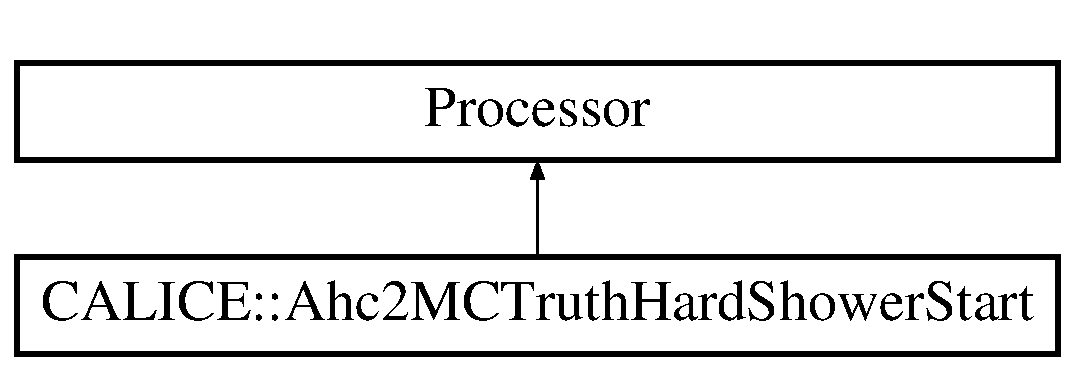
\includegraphics[height=2.000000cm]{classCALICE_1_1Ahc2MCTruthHardShowerStart}
\end{center}
\end{figure}
\subsection*{Public Member Functions}
\begin{DoxyCompactItemize}
\item 
virtual Processor $\ast$ {\bfseries new\-Processor} ()\label{classCALICE_1_1Ahc2MCTruthHardShowerStart_abeb966d2d3141cdab99397ab40e1b90f}

\item 
{\bf Ahc2\-M\-C\-Truth\-Hard\-Shower\-Start} ()
\item 
{\bf $\sim$\-Ahc2\-M\-C\-Truth\-Hard\-Shower\-Start} ()
\item 
virtual void {\bf init} ()
\item 
virtual void {\bf process\-Run\-Header} (L\-C\-Event $\ast$evt)
\item 
virtual void {\bf process\-Event} (L\-C\-Event $\ast$evt)
\item 
virtual void {\bf check} (L\-C\-Event $\ast$evt)
\item 
virtual void {\bf end} ()
\item 
void {\bfseries print\-Parameters} ()\label{classCALICE_1_1Ahc2MCTruthHardShowerStart_ab4ad83875261a47be2c11f3b966c12eb}

\end{DoxyCompactItemize}
\subsection*{Protected Attributes}
\begin{DoxyCompactItemize}
\item 
int {\bfseries \-\_\-n\-Evt}\label{classCALICE_1_1Ahc2MCTruthHardShowerStart_ae8f0eb6e9eb2cc51b8a471b4d4d3ce76}

\item 
int {\bfseries \-\_\-n\-Run}\label{classCALICE_1_1Ahc2MCTruthHardShowerStart_ae99c3a50b51c79ddac7cefbc533c850d}

\item 
unsigned int {\bfseries N\-Layer}\label{classCALICE_1_1Ahc2MCTruthHardShowerStart_a25889052fdfbe33cbef8bf9bfa7de590}

\item 
float {\bfseries pos\-Layer} [N\-L\-A\-Y\-E\-R] = \{0.\}\label{classCALICE_1_1Ahc2MCTruthHardShowerStart_a13be2c6aed919f99daeb99a212abd313}

\item 
std\-::string {\bfseries \-\_\-evt\-Var\-Col\-Name}\label{classCALICE_1_1Ahc2MCTruthHardShowerStart_a29dd4ab57d981e4fa3122d448a309675}

\item 
std\-::string {\bfseries \-\_\-hit\-In\-Col\-Name}\label{classCALICE_1_1Ahc2MCTruthHardShowerStart_a64858317a8599b865ae3b3a6d583db82}

\item 
std\-::string {\bfseries \-\_\-\-M\-C\-Particle\-Col\-Name}\label{classCALICE_1_1Ahc2MCTruthHardShowerStart_acde8084dbd0974f9449ec8868f9aef0c}

\item 
bool {\bfseries \-\_\-is\-T\-B\-May2018}\label{classCALICE_1_1Ahc2MCTruthHardShowerStart_a1d5121972e13b8b1f9be36ad4cbd025e}

\item 
bool {\bfseries \-\_\-is\-T\-B\-June2018}\label{classCALICE_1_1Ahc2MCTruthHardShowerStart_af30d7b43e5bbeb2b6e4bbdc0e364d1d1}

\item 
float {\bfseries \-\_\-hardnesscut}\label{classCALICE_1_1Ahc2MCTruthHardShowerStart_a7c49e5d94968caf6583bd4098bf77779}

\item 
int {\bfseries \-\_\-number\-Of\-M\-Cparticles}\label{classCALICE_1_1Ahc2MCTruthHardShowerStart_a6af2d800967fc3b9d7bd92189618ba9b}

\item 
int {\bfseries \-\_\-\-M\-Cpid}\label{classCALICE_1_1Ahc2MCTruthHardShowerStart_a09f3e912b0fbe24daaa3223c56ab39e2}

\item 
float {\bfseries \-\_\-\-M\-Cdecay\-Pos} [3]\label{classCALICE_1_1Ahc2MCTruthHardShowerStart_a6b2a0f33002efac67eea9566fee63934}

\item 
float {\bfseries \-\_\-hardness}\label{classCALICE_1_1Ahc2MCTruthHardShowerStart_a79a662b48b8ce608f2b37c64d437d256}

\item 
int {\bfseries \-\_\-nsecondary}\label{classCALICE_1_1Ahc2MCTruthHardShowerStart_a6ccea38c55c680df9126928d07d137c2}

\item 
unsigned int {\bfseries \-\_\-\-M\-Clayer}\label{classCALICE_1_1Ahc2MCTruthHardShowerStart_aa778b602e1c267d4d1199060b98ab0ad}

\item 
float {\bfseries st\-\_\-z}\label{classCALICE_1_1Ahc2MCTruthHardShowerStart_a2ac98f3b1ad1d7ffe2f7193d168e5819}

\item 
float {\bfseries \-\_\-esum\-\_\-secondaries}\label{classCALICE_1_1Ahc2MCTruthHardShowerStart_a72be7332d72246f211b15622df741346}

\item 
float {\bfseries \-\_\-elead}\label{classCALICE_1_1Ahc2MCTruthHardShowerStart_aaaeaa631e00af228a2cea2f2660bf1ca}

\item 
double {\bfseries mass\-\_\-primary}\label{classCALICE_1_1Ahc2MCTruthHardShowerStart_a16ecab4b80884ed402d5cf6afe65328f}

\item 
double {\bfseries mom\-\_\-daughter\-\_\-z}\label{classCALICE_1_1Ahc2MCTruthHardShowerStart_ad11e442006d2afd0421b89ed10d4a7be}

\item 
double {\bfseries mass\-\_\-daughter}\label{classCALICE_1_1Ahc2MCTruthHardShowerStart_a90b4b75671eba0d97ef01abae52e07f1}

\item 
bool {\bfseries has\-Kminus1}\label{classCALICE_1_1Ahc2MCTruthHardShowerStart_a5432d201a832211eb1cd1ccd2ba43f6d}

\item 
unsigned int {\bfseries layer}\label{classCALICE_1_1Ahc2MCTruthHardShowerStart_ab57046d15d36ea76449351376cbbf41b}

\item 
std\-::string {\bfseries \-\_\-\-Root\-Hardoutput}\label{classCALICE_1_1Ahc2MCTruthHardShowerStart_a8568c1accbb1af5cc8feea2f07fb7db7}

\end{DoxyCompactItemize}


\subsection{Constructor \& Destructor Documentation}
\index{C\-A\-L\-I\-C\-E\-::\-Ahc2\-M\-C\-Truth\-Hard\-Shower\-Start@{C\-A\-L\-I\-C\-E\-::\-Ahc2\-M\-C\-Truth\-Hard\-Shower\-Start}!Ahc2\-M\-C\-Truth\-Hard\-Shower\-Start@{Ahc2\-M\-C\-Truth\-Hard\-Shower\-Start}}
\index{Ahc2\-M\-C\-Truth\-Hard\-Shower\-Start@{Ahc2\-M\-C\-Truth\-Hard\-Shower\-Start}!CALICE::Ahc2MCTruthHardShowerStart@{C\-A\-L\-I\-C\-E\-::\-Ahc2\-M\-C\-Truth\-Hard\-Shower\-Start}}
\subsubsection[{Ahc2\-M\-C\-Truth\-Hard\-Shower\-Start}]{\setlength{\rightskip}{0pt plus 5cm}C\-A\-L\-I\-C\-E\-::\-Ahc2\-M\-C\-Truth\-Hard\-Shower\-Start\-::\-Ahc2\-M\-C\-Truth\-Hard\-Shower\-Start (
\begin{DoxyParamCaption}
{}
\end{DoxyParamCaption}
)}\label{classCALICE_1_1Ahc2MCTruthHardShowerStart_a801bf11152474ae344a18b2942885bf8}
Default constructor. \index{C\-A\-L\-I\-C\-E\-::\-Ahc2\-M\-C\-Truth\-Hard\-Shower\-Start@{C\-A\-L\-I\-C\-E\-::\-Ahc2\-M\-C\-Truth\-Hard\-Shower\-Start}!$\sim$\-Ahc2\-M\-C\-Truth\-Hard\-Shower\-Start@{$\sim$\-Ahc2\-M\-C\-Truth\-Hard\-Shower\-Start}}
\index{$\sim$\-Ahc2\-M\-C\-Truth\-Hard\-Shower\-Start@{$\sim$\-Ahc2\-M\-C\-Truth\-Hard\-Shower\-Start}!CALICE::Ahc2MCTruthHardShowerStart@{C\-A\-L\-I\-C\-E\-::\-Ahc2\-M\-C\-Truth\-Hard\-Shower\-Start}}
\subsubsection[{$\sim$\-Ahc2\-M\-C\-Truth\-Hard\-Shower\-Start}]{\setlength{\rightskip}{0pt plus 5cm}C\-A\-L\-I\-C\-E\-::\-Ahc2\-M\-C\-Truth\-Hard\-Shower\-Start\-::$\sim$\-Ahc2\-M\-C\-Truth\-Hard\-Shower\-Start (
\begin{DoxyParamCaption}
{}
\end{DoxyParamCaption}
)\hspace{0.3cm}{\ttfamily [inline]}}\label{classCALICE_1_1Ahc2MCTruthHardShowerStart_a3b2b7e3f27319ff0436527b61c6f7522}
Default destructor. 

\subsection{Member Function Documentation}
\index{C\-A\-L\-I\-C\-E\-::\-Ahc2\-M\-C\-Truth\-Hard\-Shower\-Start@{C\-A\-L\-I\-C\-E\-::\-Ahc2\-M\-C\-Truth\-Hard\-Shower\-Start}!check@{check}}
\index{check@{check}!CALICE::Ahc2MCTruthHardShowerStart@{C\-A\-L\-I\-C\-E\-::\-Ahc2\-M\-C\-Truth\-Hard\-Shower\-Start}}
\subsubsection[{check}]{\setlength{\rightskip}{0pt plus 5cm}void C\-A\-L\-I\-C\-E\-::\-Ahc2\-M\-C\-Truth\-Hard\-Shower\-Start\-::check (
\begin{DoxyParamCaption}
\item[{L\-C\-Event $\ast$}]{evt}
\end{DoxyParamCaption}
)\hspace{0.3cm}{\ttfamily [virtual]}}\label{classCALICE_1_1Ahc2MCTruthHardShowerStart_a3d954b372c03edf7ab6060f4b9167bc1}
Marlin \doxyref{check()}{p.}{classCALICE_1_1Ahc2MCTruthHardShowerStart_a3d954b372c03edf7ab6060f4b9167bc1} function. \index{C\-A\-L\-I\-C\-E\-::\-Ahc2\-M\-C\-Truth\-Hard\-Shower\-Start@{C\-A\-L\-I\-C\-E\-::\-Ahc2\-M\-C\-Truth\-Hard\-Shower\-Start}!end@{end}}
\index{end@{end}!CALICE::Ahc2MCTruthHardShowerStart@{C\-A\-L\-I\-C\-E\-::\-Ahc2\-M\-C\-Truth\-Hard\-Shower\-Start}}
\subsubsection[{end}]{\setlength{\rightskip}{0pt plus 5cm}void C\-A\-L\-I\-C\-E\-::\-Ahc2\-M\-C\-Truth\-Hard\-Shower\-Start\-::end (
\begin{DoxyParamCaption}
{}
\end{DoxyParamCaption}
)\hspace{0.3cm}{\ttfamily [virtual]}}\label{classCALICE_1_1Ahc2MCTruthHardShowerStart_aa50a7d6023510e8e8210d5de207503b4}
Marlin \doxyref{end()}{p.}{classCALICE_1_1Ahc2MCTruthHardShowerStart_aa50a7d6023510e8e8210d5de207503b4} function. 

Referenced by process\-Event().

\index{C\-A\-L\-I\-C\-E\-::\-Ahc2\-M\-C\-Truth\-Hard\-Shower\-Start@{C\-A\-L\-I\-C\-E\-::\-Ahc2\-M\-C\-Truth\-Hard\-Shower\-Start}!init@{init}}
\index{init@{init}!CALICE::Ahc2MCTruthHardShowerStart@{C\-A\-L\-I\-C\-E\-::\-Ahc2\-M\-C\-Truth\-Hard\-Shower\-Start}}
\subsubsection[{init}]{\setlength{\rightskip}{0pt plus 5cm}void C\-A\-L\-I\-C\-E\-::\-Ahc2\-M\-C\-Truth\-Hard\-Shower\-Start\-::init (
\begin{DoxyParamCaption}
{}
\end{DoxyParamCaption}
)\hspace{0.3cm}{\ttfamily [virtual]}}\label{classCALICE_1_1Ahc2MCTruthHardShowerStart_a0a2a70a8394bdd1df0ba8a5c1ecaae70}
Marlin \doxyref{init()}{p.}{classCALICE_1_1Ahc2MCTruthHardShowerStart_a0a2a70a8394bdd1df0ba8a5c1ecaae70} function. \index{C\-A\-L\-I\-C\-E\-::\-Ahc2\-M\-C\-Truth\-Hard\-Shower\-Start@{C\-A\-L\-I\-C\-E\-::\-Ahc2\-M\-C\-Truth\-Hard\-Shower\-Start}!process\-Event@{process\-Event}}
\index{process\-Event@{process\-Event}!CALICE::Ahc2MCTruthHardShowerStart@{C\-A\-L\-I\-C\-E\-::\-Ahc2\-M\-C\-Truth\-Hard\-Shower\-Start}}
\subsubsection[{process\-Event}]{\setlength{\rightskip}{0pt plus 5cm}void C\-A\-L\-I\-C\-E\-::\-Ahc2\-M\-C\-Truth\-Hard\-Shower\-Start\-::process\-Event (
\begin{DoxyParamCaption}
\item[{L\-C\-Event $\ast$}]{evt}
\end{DoxyParamCaption}
)\hspace{0.3cm}{\ttfamily [virtual]}}\label{classCALICE_1_1Ahc2MCTruthHardShowerStart_a1c7285fc225ae3972227dc4763ae0c62}
Marlin \doxyref{process\-Event()}{p.}{classCALICE_1_1Ahc2MCTruthHardShowerStart_a1c7285fc225ae3972227dc4763ae0c62} function. 

References end().

\index{C\-A\-L\-I\-C\-E\-::\-Ahc2\-M\-C\-Truth\-Hard\-Shower\-Start@{C\-A\-L\-I\-C\-E\-::\-Ahc2\-M\-C\-Truth\-Hard\-Shower\-Start}!process\-Run\-Header@{process\-Run\-Header}}
\index{process\-Run\-Header@{process\-Run\-Header}!CALICE::Ahc2MCTruthHardShowerStart@{C\-A\-L\-I\-C\-E\-::\-Ahc2\-M\-C\-Truth\-Hard\-Shower\-Start}}
\subsubsection[{process\-Run\-Header}]{\setlength{\rightskip}{0pt plus 5cm}void C\-A\-L\-I\-C\-E\-::\-Ahc2\-M\-C\-Truth\-Hard\-Shower\-Start\-::process\-Run\-Header (
\begin{DoxyParamCaption}
\item[{L\-C\-Event $\ast$}]{evt}
\end{DoxyParamCaption}
)\hspace{0.3cm}{\ttfamily [virtual]}}\label{classCALICE_1_1Ahc2MCTruthHardShowerStart_a2c40b8284f0c89f76dca1b50bbb46480}
Marlin \doxyref{process\-Run\-Header()}{p.}{classCALICE_1_1Ahc2MCTruthHardShowerStart_a2c40b8284f0c89f76dca1b50bbb46480} function. 

The documentation for this class was generated from the following files\-:\begin{DoxyCompactItemize}
\item 
/nfs/dust/ilc/user/marquezh/\-Calice\-Soft\-\_\-w\-\_\-\-I\-L\-C\-Soft\-\_\-v02-\/03-\/02/calice\-\_\-analysis/addon\-Procs/include/Ahc2\-M\-C\-Truth\-Hard\-Shower\-Start.\-hh\item 
/nfs/dust/ilc/user/marquezh/\-Calice\-Soft\-\_\-w\-\_\-\-I\-L\-C\-Soft\-\_\-v02-\/03-\/02/calice\-\_\-analysis/addon\-Procs/src/Ahc2\-M\-C\-Truth\-Hard\-Shower\-Start.\-cc\end{DoxyCompactItemize}

\section{C\-A\-L\-I\-C\-E\-:\-:Ahc\-Veto\-Region Class Reference}
\label{classCALICE_1_1AhcVetoRegion}\index{C\-A\-L\-I\-C\-E\-::\-Ahc\-Veto\-Region@{C\-A\-L\-I\-C\-E\-::\-Ahc\-Veto\-Region}}


{\ttfamily \#include $<$Ahc\-Veto\-Region.\-hh$>$}

Inheritance diagram for C\-A\-L\-I\-C\-E\-:\-:Ahc\-Veto\-Region\-:\begin{figure}[H]
\begin{center}
\leavevmode
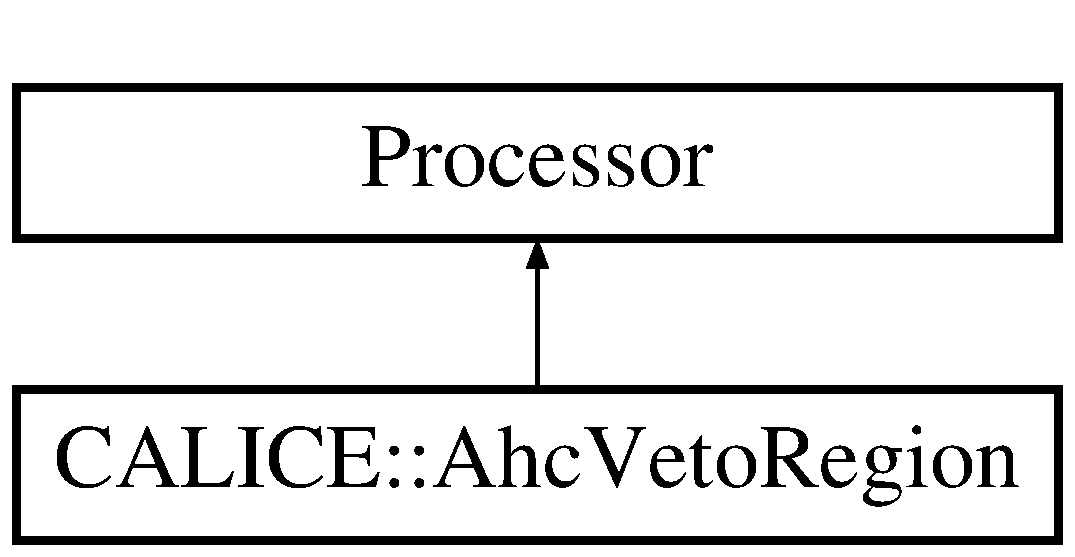
\includegraphics[height=2.000000cm]{classCALICE_1_1AhcVetoRegion}
\end{center}
\end{figure}
\subsection*{Public Member Functions}
\begin{DoxyCompactItemize}
\item 
Processor $\ast$ {\bfseries new\-Processor} ()\label{classCALICE_1_1AhcVetoRegion_a5dba726835e983d0d29e1185447a073e}

\item 
void {\bf init} ()
\item 
void {\bf process\-Run\-Header} (L\-C\-Run\-Header $\ast$run)
\item 
void {\bf process\-Event} (L\-C\-Event $\ast$evt)
\item 
void {\bf end} ()
\end{DoxyCompactItemize}
\subsection*{Protected Attributes}
\begin{DoxyCompactItemize}
\item 
std\-::string {\bfseries \-\_\-ahc\-Hit\-Col\-Name}\label{classCALICE_1_1AhcVetoRegion_aa0680886126afe8e678666fb261886df}

\item 
std\-::string {\bfseries \-\_\-mapping\-Processor\-Name}\label{classCALICE_1_1AhcVetoRegion_ac243631ab1c7f5d8f72513d39bccc9f2}

\item 
std\-::string {\bfseries \-\_\-cell\-Description\-Processor\-Name}\label{classCALICE_1_1AhcVetoRegion_a685336ec59da72ec544d2f6f1a1c9465}

\item 
Float\-Vec {\bfseries \-\_\-hit\-Threshold}\label{classCALICE_1_1AhcVetoRegion_a6fa45685bab33cf4334b9b7d29b3865e}

\item 
Int\-Vec {\bfseries \-\_\-roi\-Cells}\label{classCALICE_1_1AhcVetoRegion_a0b61c2d5dc8df3f7a4559a2070cb9a3e}

\item 
Int\-Vec {\bfseries \-\_\-roi\-First\-Layer}\label{classCALICE_1_1AhcVetoRegion_aa0d77af2ee40f113f3ddedb8c07b4690}

\item 
Int\-Vec {\bfseries \-\_\-roi\-Last\-Layer}\label{classCALICE_1_1AhcVetoRegion_a3c795f602cb3e0139040f2165ed02076}

\item 
Float\-Vec {\bfseries \-\_\-roi\-Inner\-Radius}\label{classCALICE_1_1AhcVetoRegion_aabe86778598296d8732dce74d2b7eb5c}

\item 
Float\-Vec {\bfseries \-\_\-roi\-Outer\-Radius}\label{classCALICE_1_1AhcVetoRegion_ae2eb60c0d87906b96d8adb6dda48bf9d}

\item 
Float\-Vec {\bfseries \-\_\-roi\-Inner\-Side\-Length}\label{classCALICE_1_1AhcVetoRegion_a698321a7a57e667de35447e9e8a8fcd4}

\item 
Float\-Vec {\bfseries \-\_\-roi\-Outer\-Side\-Length}\label{classCALICE_1_1AhcVetoRegion_ab96bd04a9b20053c9d9aaabe9613298b}

\item 
Int\-Vec {\bfseries \-\_\-min\-Hits}\label{classCALICE_1_1AhcVetoRegion_ad9670f0dafaf27cfeb111767970e2d0a}

\item 
Float\-Vec {\bfseries \-\_\-min\-E\-Sum}\label{classCALICE_1_1AhcVetoRegion_ab77b31a96118ff11a4ed31270b0797f0}

\item 
float {\bfseries \-\_\-roi\-Center} [2]\label{classCALICE_1_1AhcVetoRegion_a7d8a5d677ae9befa0e82968165e0cd2e}

\item 
const C\-A\-L\-I\-C\-E\-::\-Ahc\-Mapper $\ast$ {\bfseries \-\_\-mapper}\label{classCALICE_1_1AhcVetoRegion_a0ced5dc60ca9c96a3c097e8c660d94d5}

\item 
unsigned int {\bfseries \-\_\-mapper\-Version}\label{classCALICE_1_1AhcVetoRegion_abc1b667a00c9a30c1c4d81168ddbccbb}

\item 
Mapped\-Container\\*
$<$ Cell\-Description $>$ $\ast$ {\bfseries \-\_\-cell\-Descriptions}\label{classCALICE_1_1AhcVetoRegion_a4bfca4dcec6926e102c6294b8dd5c248}

\end{DoxyCompactItemize}


\subsection{Detailed Description}
Processor which generates a trigger bit based on A\-H\-C\-A\-L information. Threshold parameters are vectors, i.\-e. a series of different veto conditions can be defined for one instance of this processor. The trigger bit can be used by other processors, e.\-g. the \doxyref{Event\-Selector}{p.}{classCALICE_1_1EventSelector}. \begin{DoxyAuthor}{Author}
N. Feege 
\end{DoxyAuthor}
\begin{DoxyDate}{Date}
Aug 2009 
\end{DoxyDate}


\subsection{Member Function Documentation}
\index{C\-A\-L\-I\-C\-E\-::\-Ahc\-Veto\-Region@{C\-A\-L\-I\-C\-E\-::\-Ahc\-Veto\-Region}!end@{end}}
\index{end@{end}!CALICE::AhcVetoRegion@{C\-A\-L\-I\-C\-E\-::\-Ahc\-Veto\-Region}}
\subsubsection[{end}]{\setlength{\rightskip}{0pt plus 5cm}void C\-A\-L\-I\-C\-E\-::\-Ahc\-Veto\-Region\-::end (
\begin{DoxyParamCaption}
{}
\end{DoxyParamCaption}
)}\label{classCALICE_1_1AhcVetoRegion_a6b58441f4f4f9d28c5de32b09fdad20b}
Called after data processing for clean up. \index{C\-A\-L\-I\-C\-E\-::\-Ahc\-Veto\-Region@{C\-A\-L\-I\-C\-E\-::\-Ahc\-Veto\-Region}!init@{init}}
\index{init@{init}!CALICE::AhcVetoRegion@{C\-A\-L\-I\-C\-E\-::\-Ahc\-Veto\-Region}}
\subsubsection[{init}]{\setlength{\rightskip}{0pt plus 5cm}void C\-A\-L\-I\-C\-E\-::\-Ahc\-Veto\-Region\-::init (
\begin{DoxyParamCaption}
{}
\end{DoxyParamCaption}
)}\label{classCALICE_1_1AhcVetoRegion_a86044ed89ff5cae82065c713fb958c64}
Called at the begin of the job before anything is read. Use to initialize the processor, e.\-g. book histograms. \index{C\-A\-L\-I\-C\-E\-::\-Ahc\-Veto\-Region@{C\-A\-L\-I\-C\-E\-::\-Ahc\-Veto\-Region}!process\-Event@{process\-Event}}
\index{process\-Event@{process\-Event}!CALICE::AhcVetoRegion@{C\-A\-L\-I\-C\-E\-::\-Ahc\-Veto\-Region}}
\subsubsection[{process\-Event}]{\setlength{\rightskip}{0pt plus 5cm}void C\-A\-L\-I\-C\-E\-::\-Ahc\-Veto\-Region\-::process\-Event (
\begin{DoxyParamCaption}
\item[{L\-C\-Event $\ast$}]{evt}
\end{DoxyParamCaption}
)}\label{classCALICE_1_1AhcVetoRegion_ad909c9d1487853cefdb845e962740bad}
Called for every event -\/ this is where the real action is taking place. \index{C\-A\-L\-I\-C\-E\-::\-Ahc\-Veto\-Region@{C\-A\-L\-I\-C\-E\-::\-Ahc\-Veto\-Region}!process\-Run\-Header@{process\-Run\-Header}}
\index{process\-Run\-Header@{process\-Run\-Header}!CALICE::AhcVetoRegion@{C\-A\-L\-I\-C\-E\-::\-Ahc\-Veto\-Region}}
\subsubsection[{process\-Run\-Header}]{\setlength{\rightskip}{0pt plus 5cm}void C\-A\-L\-I\-C\-E\-::\-Ahc\-Veto\-Region\-::process\-Run\-Header (
\begin{DoxyParamCaption}
\item[{L\-C\-Run\-Header $\ast$}]{run}
\end{DoxyParamCaption}
)}\label{classCALICE_1_1AhcVetoRegion_a80e4117703d095711c05883e46704c8d}
Called for every run, e.\-g. overwrite to initialize run dependent histograms. 

The documentation for this class was generated from the following files\-:\begin{DoxyCompactItemize}
\item 
/nfs/dust/ilc/user/marquezh/\-Calice\-Soft\-\_\-w\-\_\-\-I\-L\-C\-Soft\-\_\-v02-\/03-\/02/calice\-\_\-analysis/addon\-Procs/include/Ahc\-Veto\-Region.\-hh\item 
/nfs/dust/ilc/user/marquezh/\-Calice\-Soft\-\_\-w\-\_\-\-I\-L\-C\-Soft\-\_\-v02-\/03-\/02/calice\-\_\-analysis/addon\-Procs/src/Ahc\-Veto\-Region.\-cc\end{DoxyCompactItemize}

\section{C\-A\-L\-I\-C\-E\-:\-:angle\-Track\-Finder Class Reference}
\label{classCALICE_1_1angleTrackFinder}\index{C\-A\-L\-I\-C\-E\-::angle\-Track\-Finder@{C\-A\-L\-I\-C\-E\-::angle\-Track\-Finder}}


Processor to extract M\-I\-P calibrations from muon beam runs.  




{\ttfamily \#include $<$angle\-Track\-Finder.\-hh$>$}

Inheritance diagram for C\-A\-L\-I\-C\-E\-:\-:angle\-Track\-Finder\-:\begin{figure}[H]
\begin{center}
\leavevmode
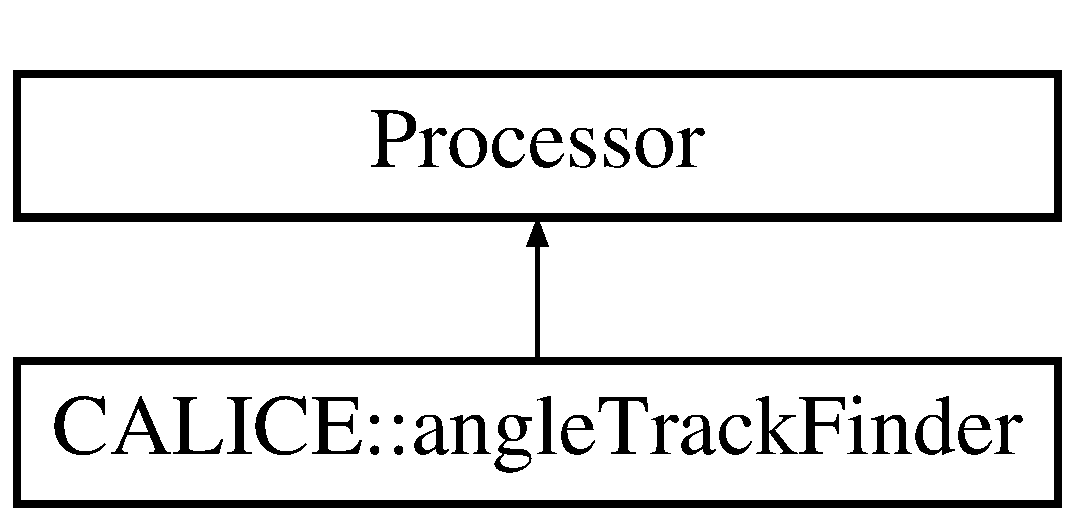
\includegraphics[height=2.000000cm]{classCALICE_1_1angleTrackFinder}
\end{center}
\end{figure}
\subsection*{Public Member Functions}
\begin{DoxyCompactItemize}
\item 
virtual Processor $\ast$ {\bf new\-Processor} ()
\item 
{\bf angle\-Track\-Finder} ()
\item 
{\bf $\sim$angle\-Track\-Finder} ()
\item 
virtual void {\bf init} ()
\item 
virtual void {\bf process\-Event} (L\-C\-Event $\ast$evt)
\item 
virtual void {\bf end} ()
\end{DoxyCompactItemize}


\subsection{Detailed Description}
Processor to extract M\-I\-P calibrations from muon beam runs. 

\begin{DoxyAuthor}{Author}
A.\-Vargas D\-E\-S\-Y 
\end{DoxyAuthor}
\begin{DoxyDate}{Date}
Jul 13 2006, 2008 
\end{DoxyDate}


\subsection{Constructor \& Destructor Documentation}
\index{C\-A\-L\-I\-C\-E\-::angle\-Track\-Finder@{C\-A\-L\-I\-C\-E\-::angle\-Track\-Finder}!angle\-Track\-Finder@{angle\-Track\-Finder}}
\index{angle\-Track\-Finder@{angle\-Track\-Finder}!CALICE::angleTrackFinder@{C\-A\-L\-I\-C\-E\-::angle\-Track\-Finder}}
\subsubsection[{angle\-Track\-Finder}]{\setlength{\rightskip}{0pt plus 5cm}C\-A\-L\-I\-C\-E\-::angle\-Track\-Finder\-::angle\-Track\-Finder (
\begin{DoxyParamCaption}
{}
\end{DoxyParamCaption}
)}\label{classCALICE_1_1angleTrackFinder_af19df480d683bb6794b10c8f601df93c}
Default constructor \index{C\-A\-L\-I\-C\-E\-::angle\-Track\-Finder@{C\-A\-L\-I\-C\-E\-::angle\-Track\-Finder}!$\sim$angle\-Track\-Finder@{$\sim$angle\-Track\-Finder}}
\index{$\sim$angle\-Track\-Finder@{$\sim$angle\-Track\-Finder}!CALICE::angleTrackFinder@{C\-A\-L\-I\-C\-E\-::angle\-Track\-Finder}}
\subsubsection[{$\sim$angle\-Track\-Finder}]{\setlength{\rightskip}{0pt plus 5cm}C\-A\-L\-I\-C\-E\-::angle\-Track\-Finder\-::$\sim$angle\-Track\-Finder (
\begin{DoxyParamCaption}
{}
\end{DoxyParamCaption}
)}\label{classCALICE_1_1angleTrackFinder_a8ceb3ec3ece38ec0a46a22d334fc08de}
Destructor 

\subsection{Member Function Documentation}
\index{C\-A\-L\-I\-C\-E\-::angle\-Track\-Finder@{C\-A\-L\-I\-C\-E\-::angle\-Track\-Finder}!end@{end}}
\index{end@{end}!CALICE::angleTrackFinder@{C\-A\-L\-I\-C\-E\-::angle\-Track\-Finder}}
\subsubsection[{end}]{\setlength{\rightskip}{0pt plus 5cm}virtual void C\-A\-L\-I\-C\-E\-::angle\-Track\-Finder\-::end (
\begin{DoxyParamCaption}
{}
\end{DoxyParamCaption}
)\hspace{0.3cm}{\ttfamily [inline]}, {\ttfamily [virtual]}}\label{classCALICE_1_1angleTrackFinder_ada7df1fe97e1ef52ed8d0a0f3109249e}
Function to be called at the end of the job, after all events have been processed, for clean up \index{C\-A\-L\-I\-C\-E\-::angle\-Track\-Finder@{C\-A\-L\-I\-C\-E\-::angle\-Track\-Finder}!init@{init}}
\index{init@{init}!CALICE::angleTrackFinder@{C\-A\-L\-I\-C\-E\-::angle\-Track\-Finder}}
\subsubsection[{init}]{\setlength{\rightskip}{0pt plus 5cm}void C\-A\-L\-I\-C\-E\-::angle\-Track\-Finder\-::init (
\begin{DoxyParamCaption}
{}
\end{DoxyParamCaption}
)\hspace{0.3cm}{\ttfamily [virtual]}}\label{classCALICE_1_1angleTrackFinder_a7fc8e11c849621452abc9d6cd7a64e1e}
Initialise useful variables \index{C\-A\-L\-I\-C\-E\-::angle\-Track\-Finder@{C\-A\-L\-I\-C\-E\-::angle\-Track\-Finder}!new\-Processor@{new\-Processor}}
\index{new\-Processor@{new\-Processor}!CALICE::angleTrackFinder@{C\-A\-L\-I\-C\-E\-::angle\-Track\-Finder}}
\subsubsection[{new\-Processor}]{\setlength{\rightskip}{0pt plus 5cm}virtual Processor$\ast$ C\-A\-L\-I\-C\-E\-::angle\-Track\-Finder\-::new\-Processor (
\begin{DoxyParamCaption}
{}
\end{DoxyParamCaption}
)\hspace{0.3cm}{\ttfamily [inline]}, {\ttfamily [virtual]}}\label{classCALICE_1_1angleTrackFinder_adceb2b658a243cea1fd8cd648986d52f}
Return new instance of this processor \index{C\-A\-L\-I\-C\-E\-::angle\-Track\-Finder@{C\-A\-L\-I\-C\-E\-::angle\-Track\-Finder}!process\-Event@{process\-Event}}
\index{process\-Event@{process\-Event}!CALICE::angleTrackFinder@{C\-A\-L\-I\-C\-E\-::angle\-Track\-Finder}}
\subsubsection[{process\-Event}]{\setlength{\rightskip}{0pt plus 5cm}void C\-A\-L\-I\-C\-E\-::angle\-Track\-Finder\-::process\-Event (
\begin{DoxyParamCaption}
\item[{L\-C\-Event $\ast$}]{evt}
\end{DoxyParamCaption}
)\hspace{0.3cm}{\ttfamily [virtual]}}\label{classCALICE_1_1angleTrackFinder_a84a7c94d5a544d204cea4bb5a4b4831c}
Process event (the working horse) 
\begin{DoxyParams}{Parameters}
{\em evt} & event to be processed \\
\hline
\end{DoxyParams}


The documentation for this class was generated from the following files\-:\begin{DoxyCompactItemize}
\item 
/nfs/dust/ilc/user/marquezh/\-Calice\-Soft\-\_\-w\-\_\-\-I\-L\-C\-Soft\-\_\-v02-\/03-\/02/calice\-\_\-analysis/addon\-Procs/include/angle\-Track\-Finder.\-hh\item 
/nfs/dust/ilc/user/marquezh/\-Calice\-Soft\-\_\-w\-\_\-\-I\-L\-C\-Soft\-\_\-v02-\/03-\/02/calice\-\_\-analysis/addon\-Procs/src/angle\-Track\-Finder.\-cc\end{DoxyCompactItemize}

\section{C\-A\-L\-I\-C\-E\-:\-:Append\-Integral\-Observables Class Reference}
\label{classCALICE_1_1AppendIntegralObservables}\index{C\-A\-L\-I\-C\-E\-::\-Append\-Integral\-Observables@{C\-A\-L\-I\-C\-E\-::\-Append\-Integral\-Observables}}


Processor for appending integral observables like energy sum per event to each event as event parameter.  




{\ttfamily \#include $<$Append\-Integral\-Observables.\-hh$>$}

Inheritance diagram for C\-A\-L\-I\-C\-E\-:\-:Append\-Integral\-Observables\-:\begin{figure}[H]
\begin{center}
\leavevmode
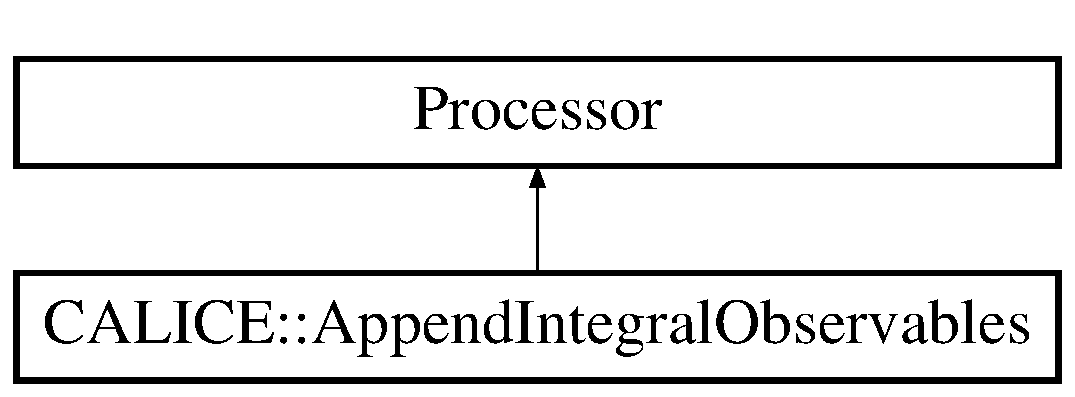
\includegraphics[height=2.000000cm]{classCALICE_1_1AppendIntegralObservables}
\end{center}
\end{figure}
\subsection*{Public Member Functions}
\begin{DoxyCompactItemize}
\item 
virtual Processor $\ast$ {\bfseries new\-Processor} ()\label{classCALICE_1_1AppendIntegralObservables_ae4e5bf5b6b635918b71198dfdcc2de41}

\item 
virtual void {\bf init} ()
\item 
virtual void {\bf process\-Run\-Header} (L\-C\-Run\-Header $\ast$run)
\item 
virtual void {\bf process\-Event} (L\-C\-Event $\ast$evt)
\item 
virtual void {\bfseries check} (L\-C\-Event $\ast$evt)\label{classCALICE_1_1AppendIntegralObservables_a6a616ca3848eefb2008f64ad2533725d}

\item 
virtual void {\bf end} ()
\end{DoxyCompactItemize}
\subsection*{Protected Attributes}
\begin{DoxyCompactItemize}
\item 
std\-::string {\bfseries \-\_\-col\-Name\-In}\label{classCALICE_1_1AppendIntegralObservables_a61277a3bfaf5170147ad4955d97b64bb}

\item 
int {\bfseries \-\_\-n\-Run}\label{classCALICE_1_1AppendIntegralObservables_a96fe79f733d56fc1abfba93f9dd507a0}

\item 
int {\bfseries \-\_\-n\-Evt}\label{classCALICE_1_1AppendIntegralObservables_a24a6b0239aeb481f2d5efd8a41704f24}

\end{DoxyCompactItemize}


\subsection{Detailed Description}
Processor for appending integral observables like energy sum per event to each event as event parameter. 

\begin{DoxyAuthor}{Author}
N. Feege, University of Hamburg 
\end{DoxyAuthor}
\begin{DoxyDate}{Date}
May 2010 
\end{DoxyDate}


\subsection{Member Function Documentation}
\index{C\-A\-L\-I\-C\-E\-::\-Append\-Integral\-Observables@{C\-A\-L\-I\-C\-E\-::\-Append\-Integral\-Observables}!end@{end}}
\index{end@{end}!CALICE::AppendIntegralObservables@{C\-A\-L\-I\-C\-E\-::\-Append\-Integral\-Observables}}
\subsubsection[{end}]{\setlength{\rightskip}{0pt plus 5cm}void C\-A\-L\-I\-C\-E\-::\-Append\-Integral\-Observables\-::end (
\begin{DoxyParamCaption}
{}
\end{DoxyParamCaption}
)\hspace{0.3cm}{\ttfamily [virtual]}}\label{classCALICE_1_1AppendIntegralObservables_a7430551409a1385ce1291b725d5e0003}
Called after data processing for clean up. \index{C\-A\-L\-I\-C\-E\-::\-Append\-Integral\-Observables@{C\-A\-L\-I\-C\-E\-::\-Append\-Integral\-Observables}!init@{init}}
\index{init@{init}!CALICE::AppendIntegralObservables@{C\-A\-L\-I\-C\-E\-::\-Append\-Integral\-Observables}}
\subsubsection[{init}]{\setlength{\rightskip}{0pt plus 5cm}void C\-A\-L\-I\-C\-E\-::\-Append\-Integral\-Observables\-::init (
\begin{DoxyParamCaption}
{}
\end{DoxyParamCaption}
)\hspace{0.3cm}{\ttfamily [virtual]}}\label{classCALICE_1_1AppendIntegralObservables_a75e4d2e19ff5c01d7a7a0e637692ee88}
Called at the begin of the job before anything is read. Use to initialize the processor, e.\-g. book histograms. \index{C\-A\-L\-I\-C\-E\-::\-Append\-Integral\-Observables@{C\-A\-L\-I\-C\-E\-::\-Append\-Integral\-Observables}!process\-Event@{process\-Event}}
\index{process\-Event@{process\-Event}!CALICE::AppendIntegralObservables@{C\-A\-L\-I\-C\-E\-::\-Append\-Integral\-Observables}}
\subsubsection[{process\-Event}]{\setlength{\rightskip}{0pt plus 5cm}void C\-A\-L\-I\-C\-E\-::\-Append\-Integral\-Observables\-::process\-Event (
\begin{DoxyParamCaption}
\item[{L\-C\-Event $\ast$}]{evt}
\end{DoxyParamCaption}
)\hspace{0.3cm}{\ttfamily [virtual]}}\label{classCALICE_1_1AppendIntegralObservables_a4cb4c0e7ab84e80068282e0fe9efd72a}
Called for every event -\/ the working horse. \index{C\-A\-L\-I\-C\-E\-::\-Append\-Integral\-Observables@{C\-A\-L\-I\-C\-E\-::\-Append\-Integral\-Observables}!process\-Run\-Header@{process\-Run\-Header}}
\index{process\-Run\-Header@{process\-Run\-Header}!CALICE::AppendIntegralObservables@{C\-A\-L\-I\-C\-E\-::\-Append\-Integral\-Observables}}
\subsubsection[{process\-Run\-Header}]{\setlength{\rightskip}{0pt plus 5cm}void C\-A\-L\-I\-C\-E\-::\-Append\-Integral\-Observables\-::process\-Run\-Header (
\begin{DoxyParamCaption}
\item[{L\-C\-Run\-Header $\ast$}]{run}
\end{DoxyParamCaption}
)\hspace{0.3cm}{\ttfamily [virtual]}}\label{classCALICE_1_1AppendIntegralObservables_ab7f95ebc7f017da0a70120f47c155f2d}
Called for every run. 

The documentation for this class was generated from the following files\-:\begin{DoxyCompactItemize}
\item 
/nfs/dust/ilc/user/marquezh/\-Calice\-Soft\-\_\-w\-\_\-\-I\-L\-C\-Soft\-\_\-v02-\/03-\/02/calice\-\_\-analysis/addon\-Procs/include/Append\-Integral\-Observables.\-hh\item 
/nfs/dust/ilc/user/marquezh/\-Calice\-Soft\-\_\-w\-\_\-\-I\-L\-C\-Soft\-\_\-v02-\/03-\/02/calice\-\_\-analysis/addon\-Procs/src/Append\-Integral\-Observables.\-cc\end{DoxyCompactItemize}

\section{C\-A\-L\-I\-C\-E\-:\-:Append\-Longitudinal\-Observables Class Reference}
\label{classCALICE_1_1AppendLongitudinalObservables}\index{C\-A\-L\-I\-C\-E\-::\-Append\-Longitudinal\-Observables@{C\-A\-L\-I\-C\-E\-::\-Append\-Longitudinal\-Observables}}


Processor for adding longitudinal observables like energy per z-\/bin to each event as event parameter.  




{\ttfamily \#include $<$Append\-Longitudinal\-Observables.\-hh$>$}

Inheritance diagram for C\-A\-L\-I\-C\-E\-:\-:Append\-Longitudinal\-Observables\-:\begin{figure}[H]
\begin{center}
\leavevmode
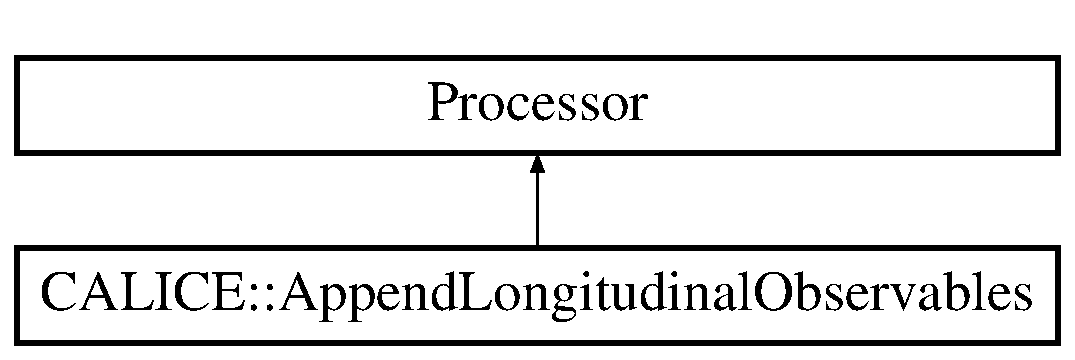
\includegraphics[height=2.000000cm]{classCALICE_1_1AppendLongitudinalObservables}
\end{center}
\end{figure}
\subsection*{Public Member Functions}
\begin{DoxyCompactItemize}
\item 
virtual Processor $\ast$ {\bfseries new\-Processor} ()\label{classCALICE_1_1AppendLongitudinalObservables_a184a5fed8c1f9e5a4dbc95f6fdb14719}

\item 
virtual void {\bf init} ()
\item 
virtual void {\bf process\-Run\-Header} (L\-C\-Run\-Header $\ast$run)
\item 
virtual void {\bf process\-Event} (L\-C\-Event $\ast$evt)
\item 
virtual void {\bfseries check} (L\-C\-Event $\ast$evt)\label{classCALICE_1_1AppendLongitudinalObservables_aecfac1c6fcaeed1f181c1e3120e0dec3}

\item 
virtual void {\bf end} ()
\end{DoxyCompactItemize}
\subsection*{Protected Attributes}
\begin{DoxyCompactItemize}
\item 
std\-::string {\bfseries \-\_\-col\-Name\-In}\label{classCALICE_1_1AppendLongitudinalObservables_ac54d2df825d928b37934be3934414c52}

\item 
std\-::string {\bfseries \-\_\-par\-Name\-Shower\-Start\-Pos}\label{classCALICE_1_1AppendLongitudinalObservables_a9bad51c48a3bde69262b4e638d6c81dd}

\item 
std\-::string {\bfseries \-\_\-par\-Name\-C\-O\-G}\label{classCALICE_1_1AppendLongitudinalObservables_a39e04e4a5a77c39ebd68d045e1a8013f}

\item 
std\-::string {\bfseries \-\_\-cell\-I\-D\-Encoding}\label{classCALICE_1_1AppendLongitudinalObservables_a55ef9352f95cf34642d4f305ceeffe6a}

\item 
std\-::string {\bfseries \-\_\-mapping\-Processor\-Name}\label{classCALICE_1_1AppendLongitudinalObservables_a6f5c538df04d53bbf30b9df32f67cc4e}

\item 
std\-::string {\bfseries \-\_\-cell\-Description\-Processor\-Name}\label{classCALICE_1_1AppendLongitudinalObservables_af7c86ff99ff1ba90fddde54aff75daa8}

\item 
int {\bfseries \-\_\-n\-Run}\label{classCALICE_1_1AppendLongitudinalObservables_a6c7d777eda786e1291259ee1c616475b}

\item 
int {\bfseries \-\_\-n\-Evt}\label{classCALICE_1_1AppendLongitudinalObservables_ac45ead0d4eee97d87e1a6a37b4273035}

\item 
const C\-A\-L\-I\-C\-E\-::\-Mapper $\ast$ {\bfseries \-\_\-mapper}\label{classCALICE_1_1AppendLongitudinalObservables_a399374c0a4467541baeb42870e268adb}

\item 
unsigned int {\bfseries \-\_\-mapper\-Version}\label{classCALICE_1_1AppendLongitudinalObservables_aa0c38d61ab94c36b64f61f304ad7bf35}

\item 
C\-A\-L\-I\-C\-E\-::\-Mapped\-Container\\*
$<$ C\-A\-L\-I\-C\-E\-::\-Cell\-Description $>$ $\ast$ {\bfseries \-\_\-cell\-Descriptions}\label{classCALICE_1_1AppendLongitudinalObservables_a4d64b00da8ba4464224d89e60951503a}

\end{DoxyCompactItemize}


\subsection{Detailed Description}
Processor for adding longitudinal observables like energy per z-\/bin to each event as event parameter. 

\begin{DoxyAuthor}{Author}
N. Feege, University of Hamburg 
\end{DoxyAuthor}
\begin{DoxyDate}{Date}
Dec 2010 
\end{DoxyDate}


\subsection{Member Function Documentation}
\index{C\-A\-L\-I\-C\-E\-::\-Append\-Longitudinal\-Observables@{C\-A\-L\-I\-C\-E\-::\-Append\-Longitudinal\-Observables}!end@{end}}
\index{end@{end}!CALICE::AppendLongitudinalObservables@{C\-A\-L\-I\-C\-E\-::\-Append\-Longitudinal\-Observables}}
\subsubsection[{end}]{\setlength{\rightskip}{0pt plus 5cm}void C\-A\-L\-I\-C\-E\-::\-Append\-Longitudinal\-Observables\-::end (
\begin{DoxyParamCaption}
{}
\end{DoxyParamCaption}
)\hspace{0.3cm}{\ttfamily [virtual]}}\label{classCALICE_1_1AppendLongitudinalObservables_aa1c159a27af81e1ee584868c04cd822c}
Called after data processing for clean up. \index{C\-A\-L\-I\-C\-E\-::\-Append\-Longitudinal\-Observables@{C\-A\-L\-I\-C\-E\-::\-Append\-Longitudinal\-Observables}!init@{init}}
\index{init@{init}!CALICE::AppendLongitudinalObservables@{C\-A\-L\-I\-C\-E\-::\-Append\-Longitudinal\-Observables}}
\subsubsection[{init}]{\setlength{\rightskip}{0pt plus 5cm}void C\-A\-L\-I\-C\-E\-::\-Append\-Longitudinal\-Observables\-::init (
\begin{DoxyParamCaption}
{}
\end{DoxyParamCaption}
)\hspace{0.3cm}{\ttfamily [virtual]}}\label{classCALICE_1_1AppendLongitudinalObservables_a34a3ca7645da9f35060d542679293ce4}
Called at the begin of the job before anything is read. Use to initialize the processor, e.\-g. book histograms. \index{C\-A\-L\-I\-C\-E\-::\-Append\-Longitudinal\-Observables@{C\-A\-L\-I\-C\-E\-::\-Append\-Longitudinal\-Observables}!process\-Event@{process\-Event}}
\index{process\-Event@{process\-Event}!CALICE::AppendLongitudinalObservables@{C\-A\-L\-I\-C\-E\-::\-Append\-Longitudinal\-Observables}}
\subsubsection[{process\-Event}]{\setlength{\rightskip}{0pt plus 5cm}void C\-A\-L\-I\-C\-E\-::\-Append\-Longitudinal\-Observables\-::process\-Event (
\begin{DoxyParamCaption}
\item[{L\-C\-Event $\ast$}]{evt}
\end{DoxyParamCaption}
)\hspace{0.3cm}{\ttfamily [virtual]}}\label{classCALICE_1_1AppendLongitudinalObservables_a17ed8fe97f4343669969340c5844e3d9}
Called for every event -\/ the working horse. \index{C\-A\-L\-I\-C\-E\-::\-Append\-Longitudinal\-Observables@{C\-A\-L\-I\-C\-E\-::\-Append\-Longitudinal\-Observables}!process\-Run\-Header@{process\-Run\-Header}}
\index{process\-Run\-Header@{process\-Run\-Header}!CALICE::AppendLongitudinalObservables@{C\-A\-L\-I\-C\-E\-::\-Append\-Longitudinal\-Observables}}
\subsubsection[{process\-Run\-Header}]{\setlength{\rightskip}{0pt plus 5cm}void C\-A\-L\-I\-C\-E\-::\-Append\-Longitudinal\-Observables\-::process\-Run\-Header (
\begin{DoxyParamCaption}
\item[{L\-C\-Run\-Header $\ast$}]{run}
\end{DoxyParamCaption}
)\hspace{0.3cm}{\ttfamily [virtual]}}\label{classCALICE_1_1AppendLongitudinalObservables_ae6f2cc07f85acbf725aaf339420e6308}
Called for every run. 

The documentation for this class was generated from the following files\-:\begin{DoxyCompactItemize}
\item 
/nfs/dust/ilc/user/marquezh/\-Calice\-Soft\-\_\-w\-\_\-\-I\-L\-C\-Soft\-\_\-v02-\/03-\/02/calice\-\_\-analysis/addon\-Procs/include/Append\-Longitudinal\-Observables.\-hh\item 
/nfs/dust/ilc/user/marquezh/\-Calice\-Soft\-\_\-w\-\_\-\-I\-L\-C\-Soft\-\_\-v02-\/03-\/02/calice\-\_\-analysis/addon\-Procs/src/Append\-Longitudinal\-Observables.\-cc\end{DoxyCompactItemize}

\section{C\-A\-L\-I\-C\-E\-:\-:Append\-M\-C\-Particle\-Information Class Reference}
\label{classCALICE_1_1AppendMCParticleInformation}\index{C\-A\-L\-I\-C\-E\-::\-Append\-M\-C\-Particle\-Information@{C\-A\-L\-I\-C\-E\-::\-Append\-M\-C\-Particle\-Information}}


Processor for appending information about the M\-C-\/\-Particle to the event as event parameter.  




{\ttfamily \#include $<$Append\-M\-C\-Particle\-Information.\-hh$>$}

Inheritance diagram for C\-A\-L\-I\-C\-E\-:\-:Append\-M\-C\-Particle\-Information\-:\begin{figure}[H]
\begin{center}
\leavevmode
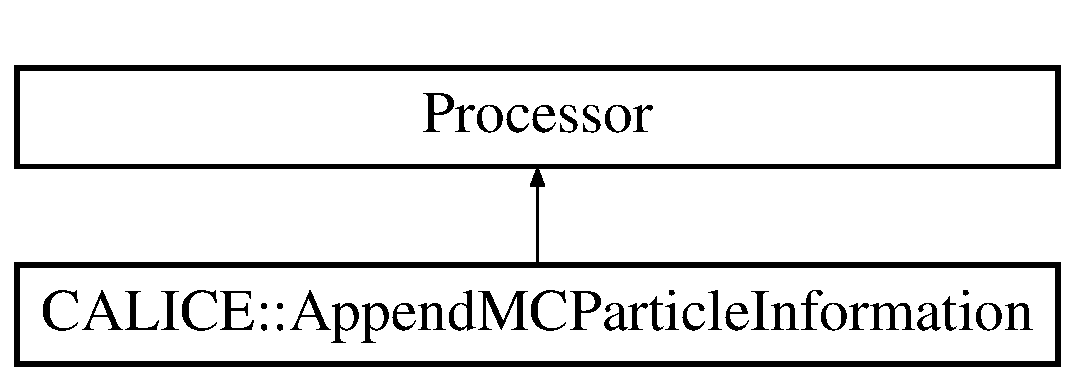
\includegraphics[height=2.000000cm]{classCALICE_1_1AppendMCParticleInformation}
\end{center}
\end{figure}
\subsection*{Public Member Functions}
\begin{DoxyCompactItemize}
\item 
virtual Processor $\ast$ {\bfseries new\-Processor} ()\label{classCALICE_1_1AppendMCParticleInformation_a960af39ab4aec5c86924c8d0ced063dc}

\item 
virtual void {\bf init} ()
\item 
virtual void {\bf process\-Run\-Header} (L\-C\-Run\-Header $\ast$run)
\item 
virtual void {\bf process\-Event} (L\-C\-Event $\ast$evt)
\item 
virtual void {\bfseries check} (L\-C\-Event $\ast$evt)\label{classCALICE_1_1AppendMCParticleInformation_accaf96eba448c6c9005f329e8d1aa10c}

\item 
virtual void {\bf end} ()
\end{DoxyCompactItemize}
\subsection*{Protected Attributes}
\begin{DoxyCompactItemize}
\item 
std\-::string {\bfseries \-\_\-col\-Name\-In}\label{classCALICE_1_1AppendMCParticleInformation_a7166f2cbd6aeccb317131f1b6578f945}

\item 
std\-::string {\bfseries \-\_\-cell\-I\-D\-Encoding}\label{classCALICE_1_1AppendMCParticleInformation_a6bb63d9cf269d9a4211a76ceff5fd32e}

\item 
std\-::string {\bfseries \-\_\-mapping\-Processor\-Name}\label{classCALICE_1_1AppendMCParticleInformation_ad1b80810b8e0de330676044e0c6e4fd6}

\item 
std\-::string {\bfseries \-\_\-cell\-Description\-Processor\-Name}\label{classCALICE_1_1AppendMCParticleInformation_a94201a45224b1c6817cefcae24f58d12}

\item 
int {\bfseries \-\_\-n\-Run}\label{classCALICE_1_1AppendMCParticleInformation_a261e3260ab61279cbc74c61c7103c098}

\item 
int {\bfseries \-\_\-n\-Evt}\label{classCALICE_1_1AppendMCParticleInformation_a94b6171871d2e0f4d1833c89b7a54d93}

\item 
const C\-A\-L\-I\-C\-E\-::\-Mapper $\ast$ {\bfseries \-\_\-mapper}\label{classCALICE_1_1AppendMCParticleInformation_af50d0e10a2da2aed02d51b4bc19817c5}

\item 
unsigned int {\bfseries \-\_\-mapper\-Version}\label{classCALICE_1_1AppendMCParticleInformation_a9b5d220515549d9b7989e9c7fd7d74c1}

\item 
C\-A\-L\-I\-C\-E\-::\-Mapped\-Container\\*
$<$ C\-A\-L\-I\-C\-E\-::\-Cell\-Description $>$ $\ast$ {\bfseries \-\_\-cell\-Descriptions}\label{classCALICE_1_1AppendMCParticleInformation_ae56390007bed950d4bb042c41dcf258e}

\end{DoxyCompactItemize}


\subsection{Detailed Description}
Processor for appending information about the M\-C-\/\-Particle to the event as event parameter. 

\begin{DoxyAuthor}{Author}
N. Feege, University of Hamburg 
\end{DoxyAuthor}
\begin{DoxyDate}{Date}
Dec 2010 
\end{DoxyDate}


\subsection{Member Function Documentation}
\index{C\-A\-L\-I\-C\-E\-::\-Append\-M\-C\-Particle\-Information@{C\-A\-L\-I\-C\-E\-::\-Append\-M\-C\-Particle\-Information}!end@{end}}
\index{end@{end}!CALICE::AppendMCParticleInformation@{C\-A\-L\-I\-C\-E\-::\-Append\-M\-C\-Particle\-Information}}
\subsubsection[{end}]{\setlength{\rightskip}{0pt plus 5cm}void C\-A\-L\-I\-C\-E\-::\-Append\-M\-C\-Particle\-Information\-::end (
\begin{DoxyParamCaption}
{}
\end{DoxyParamCaption}
)\hspace{0.3cm}{\ttfamily [virtual]}}\label{classCALICE_1_1AppendMCParticleInformation_a565be189df44151356a5f4ac62dba2c7}
Called after data processing for clean up. \index{C\-A\-L\-I\-C\-E\-::\-Append\-M\-C\-Particle\-Information@{C\-A\-L\-I\-C\-E\-::\-Append\-M\-C\-Particle\-Information}!init@{init}}
\index{init@{init}!CALICE::AppendMCParticleInformation@{C\-A\-L\-I\-C\-E\-::\-Append\-M\-C\-Particle\-Information}}
\subsubsection[{init}]{\setlength{\rightskip}{0pt plus 5cm}void C\-A\-L\-I\-C\-E\-::\-Append\-M\-C\-Particle\-Information\-::init (
\begin{DoxyParamCaption}
{}
\end{DoxyParamCaption}
)\hspace{0.3cm}{\ttfamily [virtual]}}\label{classCALICE_1_1AppendMCParticleInformation_ab9a34c59f29849b089ce3609deb43854}
Called at the begin of the job before anything is read. Use to initialize the processor, e.\-g. book histograms. \index{C\-A\-L\-I\-C\-E\-::\-Append\-M\-C\-Particle\-Information@{C\-A\-L\-I\-C\-E\-::\-Append\-M\-C\-Particle\-Information}!process\-Event@{process\-Event}}
\index{process\-Event@{process\-Event}!CALICE::AppendMCParticleInformation@{C\-A\-L\-I\-C\-E\-::\-Append\-M\-C\-Particle\-Information}}
\subsubsection[{process\-Event}]{\setlength{\rightskip}{0pt plus 5cm}void C\-A\-L\-I\-C\-E\-::\-Append\-M\-C\-Particle\-Information\-::process\-Event (
\begin{DoxyParamCaption}
\item[{L\-C\-Event $\ast$}]{evt}
\end{DoxyParamCaption}
)\hspace{0.3cm}{\ttfamily [virtual]}}\label{classCALICE_1_1AppendMCParticleInformation_a76a94373b910848b9faccb5f3699b424}
Called for every event -\/ the working horse. \index{C\-A\-L\-I\-C\-E\-::\-Append\-M\-C\-Particle\-Information@{C\-A\-L\-I\-C\-E\-::\-Append\-M\-C\-Particle\-Information}!process\-Run\-Header@{process\-Run\-Header}}
\index{process\-Run\-Header@{process\-Run\-Header}!CALICE::AppendMCParticleInformation@{C\-A\-L\-I\-C\-E\-::\-Append\-M\-C\-Particle\-Information}}
\subsubsection[{process\-Run\-Header}]{\setlength{\rightskip}{0pt plus 5cm}void C\-A\-L\-I\-C\-E\-::\-Append\-M\-C\-Particle\-Information\-::process\-Run\-Header (
\begin{DoxyParamCaption}
\item[{L\-C\-Run\-Header $\ast$}]{run}
\end{DoxyParamCaption}
)\hspace{0.3cm}{\ttfamily [virtual]}}\label{classCALICE_1_1AppendMCParticleInformation_a80c4d2d1823898eba05bd031694aa7d3}
Called for every run. 

The documentation for this class was generated from the following files\-:\begin{DoxyCompactItemize}
\item 
/nfs/dust/ilc/user/marquezh/\-Calice\-Soft\-\_\-w\-\_\-\-I\-L\-C\-Soft\-\_\-v02-\/03-\/02/calice\-\_\-analysis/addon\-Procs/include/Append\-M\-C\-Particle\-Information.\-hh\item 
/nfs/dust/ilc/user/marquezh/\-Calice\-Soft\-\_\-w\-\_\-\-I\-L\-C\-Soft\-\_\-v02-\/03-\/02/calice\-\_\-analysis/addon\-Procs/src/Append\-M\-C\-Particle\-Information.\-cc\end{DoxyCompactItemize}

\section{C\-A\-L\-I\-C\-E\-:\-:Apply\-Threshold\-Cut Class Reference}
\label{classCALICE_1_1ApplyThresholdCut}\index{C\-A\-L\-I\-C\-E\-::\-Apply\-Threshold\-Cut@{C\-A\-L\-I\-C\-E\-::\-Apply\-Threshold\-Cut}}


{\ttfamily \#include $<$Apply\-Threshold\-Cut.\-hh$>$}

Inheritance diagram for C\-A\-L\-I\-C\-E\-:\-:Apply\-Threshold\-Cut\-:\begin{figure}[H]
\begin{center}
\leavevmode
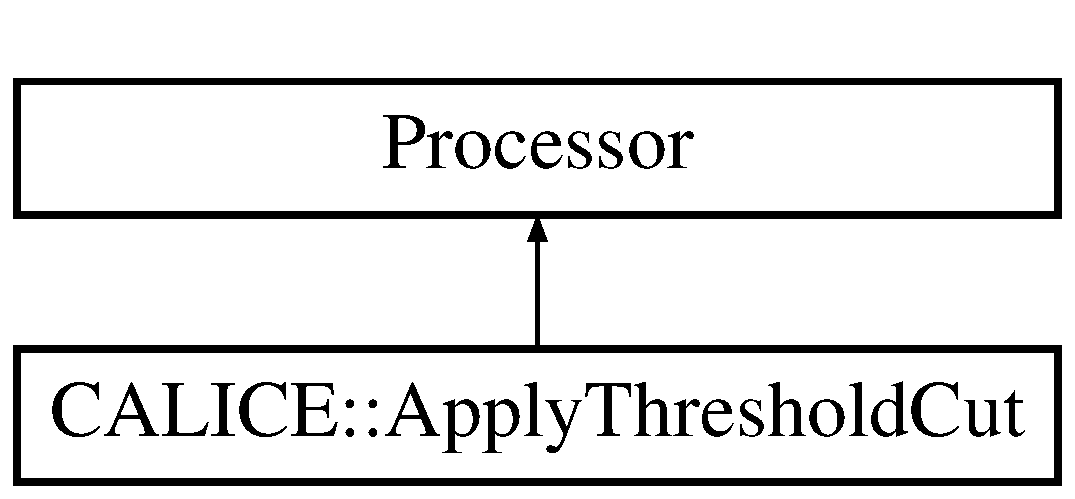
\includegraphics[height=2.000000cm]{classCALICE_1_1ApplyThresholdCut}
\end{center}
\end{figure}
\subsection*{Public Member Functions}
\begin{DoxyCompactItemize}
\item 
Processor $\ast$ {\bfseries new\-Processor} ()\label{classCALICE_1_1ApplyThresholdCut_a186bcbb2561cf335e460c21bdc0eefe7}

\item 
void {\bf init} ()
\item 
void {\bf process\-Run\-Header} (L\-C\-Run\-Header $\ast$run)
\item 
void {\bf process\-Event} (L\-C\-Event $\ast$evt)
\item 
void {\bf end} ()
\end{DoxyCompactItemize}
\subsection*{Protected Attributes}
\begin{DoxyCompactItemize}
\item 
std\-::string {\bfseries \-\_\-ahc\-Hit\-Col\-Name\-\_\-no\-Cut}\label{classCALICE_1_1ApplyThresholdCut_a844fedf3de23644cf4db571eae6371aa}

\item 
std\-::string {\bfseries \-\_\-ahc\-Hit\-Col\-Name\-\_\-w\-Cut}\label{classCALICE_1_1ApplyThresholdCut_a1879defe52c594609139e00e879cad16}

\item 
float {\bfseries \-\_\-mip\-Cut}\label{classCALICE_1_1ApplyThresholdCut_ae80630b09af37e6284350c7a85ca4d0f}

\end{DoxyCompactItemize}


\subsection{Detailed Description}
Processor which drops all hits below energy threshold from hit collection. \begin{DoxyAuthor}{Author}
N. Feege 
\end{DoxyAuthor}
\begin{DoxyDate}{Date}
Aug 2009 
\end{DoxyDate}


\subsection{Member Function Documentation}
\index{C\-A\-L\-I\-C\-E\-::\-Apply\-Threshold\-Cut@{C\-A\-L\-I\-C\-E\-::\-Apply\-Threshold\-Cut}!end@{end}}
\index{end@{end}!CALICE::ApplyThresholdCut@{C\-A\-L\-I\-C\-E\-::\-Apply\-Threshold\-Cut}}
\subsubsection[{end}]{\setlength{\rightskip}{0pt plus 5cm}void C\-A\-L\-I\-C\-E\-::\-Apply\-Threshold\-Cut\-::end (
\begin{DoxyParamCaption}
{}
\end{DoxyParamCaption}
)}\label{classCALICE_1_1ApplyThresholdCut_ad825513827e95fa0df396780b3d05821}
Called after data processing for clean up. \index{C\-A\-L\-I\-C\-E\-::\-Apply\-Threshold\-Cut@{C\-A\-L\-I\-C\-E\-::\-Apply\-Threshold\-Cut}!init@{init}}
\index{init@{init}!CALICE::ApplyThresholdCut@{C\-A\-L\-I\-C\-E\-::\-Apply\-Threshold\-Cut}}
\subsubsection[{init}]{\setlength{\rightskip}{0pt plus 5cm}void C\-A\-L\-I\-C\-E\-::\-Apply\-Threshold\-Cut\-::init (
\begin{DoxyParamCaption}
{}
\end{DoxyParamCaption}
)}\label{classCALICE_1_1ApplyThresholdCut_ab53ec0d15116404ea639ba029fbef85b}
Called at the begin of the job before anything is read. Use to initialize the processor, e.\-g. book histograms. \index{C\-A\-L\-I\-C\-E\-::\-Apply\-Threshold\-Cut@{C\-A\-L\-I\-C\-E\-::\-Apply\-Threshold\-Cut}!process\-Event@{process\-Event}}
\index{process\-Event@{process\-Event}!CALICE::ApplyThresholdCut@{C\-A\-L\-I\-C\-E\-::\-Apply\-Threshold\-Cut}}
\subsubsection[{process\-Event}]{\setlength{\rightskip}{0pt plus 5cm}void C\-A\-L\-I\-C\-E\-::\-Apply\-Threshold\-Cut\-::process\-Event (
\begin{DoxyParamCaption}
\item[{L\-C\-Event $\ast$}]{evt}
\end{DoxyParamCaption}
)}\label{classCALICE_1_1ApplyThresholdCut_ae2614ec21f7d006f3631ae6791f3ce1c}
Called for every event -\/ this is where the real action is taking place. \index{C\-A\-L\-I\-C\-E\-::\-Apply\-Threshold\-Cut@{C\-A\-L\-I\-C\-E\-::\-Apply\-Threshold\-Cut}!process\-Run\-Header@{process\-Run\-Header}}
\index{process\-Run\-Header@{process\-Run\-Header}!CALICE::ApplyThresholdCut@{C\-A\-L\-I\-C\-E\-::\-Apply\-Threshold\-Cut}}
\subsubsection[{process\-Run\-Header}]{\setlength{\rightskip}{0pt plus 5cm}void C\-A\-L\-I\-C\-E\-::\-Apply\-Threshold\-Cut\-::process\-Run\-Header (
\begin{DoxyParamCaption}
\item[{L\-C\-Run\-Header $\ast$}]{run}
\end{DoxyParamCaption}
)}\label{classCALICE_1_1ApplyThresholdCut_ae55688cdf7c7f933d64d8ca952ed3943}
Called for every run, e.\-g. overwrite to initialize run dependent histograms. 

The documentation for this class was generated from the following files\-:\begin{DoxyCompactItemize}
\item 
/nfs/dust/ilc/user/marquezh/\-Calice\-Soft\-\_\-w\-\_\-\-I\-L\-C\-Soft\-\_\-v02-\/03-\/02/calice\-\_\-analysis/addon\-Procs/include/Apply\-Threshold\-Cut.\-hh\item 
/nfs/dust/ilc/user/marquezh/\-Calice\-Soft\-\_\-w\-\_\-\-I\-L\-C\-Soft\-\_\-v02-\/03-\/02/calice\-\_\-analysis/addon\-Procs/src/Apply\-Threshold\-Cut.\-cc\end{DoxyCompactItemize}

\section{C\-A\-L\-I\-C\-E\-Overlay\-Preparation Class Reference}
\label{classCALICEOverlayPreparation}\index{C\-A\-L\-I\-C\-E\-Overlay\-Preparation@{C\-A\-L\-I\-C\-E\-Overlay\-Preparation}}


{\ttfamily \#include $<$C\-A\-L\-I\-C\-E\-Overlay\-Preparation.\-hh$>$}

Inheritance diagram for C\-A\-L\-I\-C\-E\-Overlay\-Preparation\-:\begin{figure}[H]
\begin{center}
\leavevmode
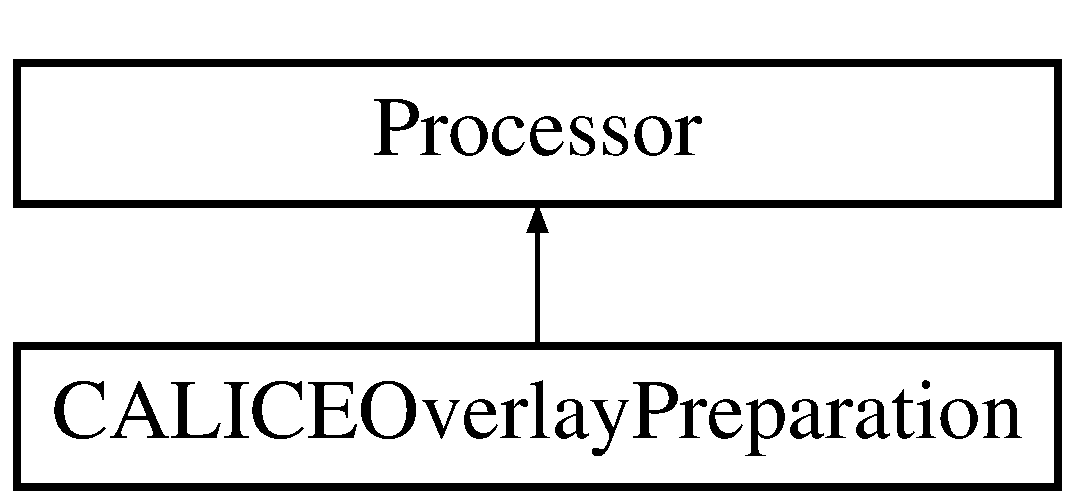
\includegraphics[height=2.000000cm]{classCALICEOverlayPreparation}
\end{center}
\end{figure}
\subsection*{Public Member Functions}
\begin{DoxyCompactItemize}
\item 
{\bf C\-A\-L\-I\-C\-E\-Overlay\-Preparation} ()
\item 
virtual {\bf $\sim$\-C\-A\-L\-I\-C\-E\-Overlay\-Preparation} ()
\item 
{\bf C\-A\-L\-I\-C\-E\-Overlay\-Preparation} $\ast$ {\bfseries new\-Processor} ()\label{classCALICEOverlayPreparation_a0198d93bc883b43dc38259ab6a94f284}

\item 
virtual void {\bf init} ()
\item 
virtual void {\bf process\-Run\-Header} (L\-C\-Run\-Header $\ast$run)
\item 
virtual void {\bf process\-Event} (lcio\-::\-L\-C\-Event $\ast$)
\item 
virtual void {\bf end} ()
\item 
unsigned {\bf get\-Starting\-Layer} ({\bf C\-Layer} $\ast$)
\begin{DoxyCompactList}\small\item\em First interaction layer and primary track finder. \end{DoxyCompactList}\item 
bool {\bf Find\-Track} (unsigned, {\bf C\-Layer} $\ast$)
\item 
bool {\bf is\-Muon} (float, float)
\item 
bool {\bf is\-Trash} (unsigned, float)
\begin{DoxyCompactList}\small\item\em C\-A\-L\-I\-C\-E event selection (muon and trash) \end{DoxyCompactList}\item 
float {\bf dist\-X\-Y} ({\bf C\-Hit} $\ast$, {\bf C\-Hit} $\ast$)
\end{DoxyCompactItemize}


\subsection{Detailed Description}
\doxyref{C\-A\-L\-I\-C\-E\-Overlay\-Preparation}{p.}{classCALICEOverlayPreparation} processor class 

\subsection{Constructor \& Destructor Documentation}
\index{C\-A\-L\-I\-C\-E\-Overlay\-Preparation@{C\-A\-L\-I\-C\-E\-Overlay\-Preparation}!C\-A\-L\-I\-C\-E\-Overlay\-Preparation@{C\-A\-L\-I\-C\-E\-Overlay\-Preparation}}
\index{C\-A\-L\-I\-C\-E\-Overlay\-Preparation@{C\-A\-L\-I\-C\-E\-Overlay\-Preparation}!CALICEOverlayPreparation@{C\-A\-L\-I\-C\-E\-Overlay\-Preparation}}
\subsubsection[{C\-A\-L\-I\-C\-E\-Overlay\-Preparation}]{\setlength{\rightskip}{0pt plus 5cm}C\-A\-L\-I\-C\-E\-Overlay\-Preparation\-::\-C\-A\-L\-I\-C\-E\-Overlay\-Preparation (
\begin{DoxyParamCaption}
{}
\end{DoxyParamCaption}
)}\label{classCALICEOverlayPreparation_a6325cb0f466f43c21161a0bdc6fc0a04}
Default constructor \index{C\-A\-L\-I\-C\-E\-Overlay\-Preparation@{C\-A\-L\-I\-C\-E\-Overlay\-Preparation}!$\sim$\-C\-A\-L\-I\-C\-E\-Overlay\-Preparation@{$\sim$\-C\-A\-L\-I\-C\-E\-Overlay\-Preparation}}
\index{$\sim$\-C\-A\-L\-I\-C\-E\-Overlay\-Preparation@{$\sim$\-C\-A\-L\-I\-C\-E\-Overlay\-Preparation}!CALICEOverlayPreparation@{C\-A\-L\-I\-C\-E\-Overlay\-Preparation}}
\subsubsection[{$\sim$\-C\-A\-L\-I\-C\-E\-Overlay\-Preparation}]{\setlength{\rightskip}{0pt plus 5cm}C\-A\-L\-I\-C\-E\-Overlay\-Preparation\-::$\sim$\-C\-A\-L\-I\-C\-E\-Overlay\-Preparation (
\begin{DoxyParamCaption}
{}
\end{DoxyParamCaption}
)\hspace{0.3cm}{\ttfamily [virtual]}}\label{classCALICEOverlayPreparation_a5fac9b3ffd811224012ea3143c67dfca}
Default destructor 

\subsection{Member Function Documentation}
\index{C\-A\-L\-I\-C\-E\-Overlay\-Preparation@{C\-A\-L\-I\-C\-E\-Overlay\-Preparation}!dist\-X\-Y@{dist\-X\-Y}}
\index{dist\-X\-Y@{dist\-X\-Y}!CALICEOverlayPreparation@{C\-A\-L\-I\-C\-E\-Overlay\-Preparation}}
\subsubsection[{dist\-X\-Y}]{\setlength{\rightskip}{0pt plus 5cm}float C\-A\-L\-I\-C\-E\-Overlay\-Preparation\-::dist\-X\-Y (
\begin{DoxyParamCaption}
\item[{{\bf C\-Hit} $\ast$}]{h1, }
\item[{{\bf C\-Hit} $\ast$}]{h2}
\end{DoxyParamCaption}
)}\label{classCALICEOverlayPreparation_a34c5ffe86d2fa90a21513612a1d036ad}
Calculates and returns distance between two hits in X\-Y-\/plane 

References C\-Hit\-::x, and C\-Hit\-::y.



Referenced by Find\-Track().

\index{C\-A\-L\-I\-C\-E\-Overlay\-Preparation@{C\-A\-L\-I\-C\-E\-Overlay\-Preparation}!end@{end}}
\index{end@{end}!CALICEOverlayPreparation@{C\-A\-L\-I\-C\-E\-Overlay\-Preparation}}
\subsubsection[{end}]{\setlength{\rightskip}{0pt plus 5cm}void C\-A\-L\-I\-C\-E\-Overlay\-Preparation\-::end (
\begin{DoxyParamCaption}
{}
\end{DoxyParamCaption}
)\hspace{0.3cm}{\ttfamily [virtual]}}\label{classCALICEOverlayPreparation_a2d8e0b68e0e5c573dfdc63755a7c9ad6}
Function to close root-\/file and print some statistic results \index{C\-A\-L\-I\-C\-E\-Overlay\-Preparation@{C\-A\-L\-I\-C\-E\-Overlay\-Preparation}!Find\-Track@{Find\-Track}}
\index{Find\-Track@{Find\-Track}!CALICEOverlayPreparation@{C\-A\-L\-I\-C\-E\-Overlay\-Preparation}}
\subsubsection[{Find\-Track}]{\setlength{\rightskip}{0pt plus 5cm}bool C\-A\-L\-I\-C\-E\-Overlay\-Preparation\-::\-Find\-Track (
\begin{DoxyParamCaption}
\item[{unsigned}]{start, }
\item[{{\bf C\-Layer} $\ast$}]{lr}
\end{DoxyParamCaption}
)}\label{classCALICEOverlayPreparation_a1536aa77e504e4e32fd0477010519946}
Finds hits belonging to primary track taking in account the earlier found shower starting point. The \char`\"{}nearest neighbour\char`\"{} criteria is used. Maximum distance parameters are defined taking in account the cell size. First parameter is the number of shower starting layer. Second parameter is an array with objects \doxyref{C\-Layer}{p.}{classCLayer} that contain layer parameters. 

References C\-Hit\-::b, dist\-X\-Y(), C\-Hit\-::l, C\-Hit\-::r, C\-Hit\-::x, C\-Hit\-::y, and C\-Hit\-::z.



Referenced by process\-Event().

\index{C\-A\-L\-I\-C\-E\-Overlay\-Preparation@{C\-A\-L\-I\-C\-E\-Overlay\-Preparation}!get\-Starting\-Layer@{get\-Starting\-Layer}}
\index{get\-Starting\-Layer@{get\-Starting\-Layer}!CALICEOverlayPreparation@{C\-A\-L\-I\-C\-E\-Overlay\-Preparation}}
\subsubsection[{get\-Starting\-Layer}]{\setlength{\rightskip}{0pt plus 5cm}unsigned C\-A\-L\-I\-C\-E\-Overlay\-Preparation\-::get\-Starting\-Layer (
\begin{DoxyParamCaption}
\item[{{\bf C\-Layer} $\ast$}]{lr}
\end{DoxyParamCaption}
)}\label{classCALICEOverlayPreparation_af24a0d57bdbaed18214f7fe98bf58e0b}


First interaction layer and primary track finder. 

Finds and returns the number of layer where shower started using the following criteria\-:
\begin{DoxyEnumerate}
\item Moving average sum of M\-I\-Ps inside the window = 10 layers for two successive layers is greater than \-\_\-av\-M\-I\-Pxxxx value.
\item Number of hits in two consequent layers is greater than \-\_\-hit\-Limxxx value. Both constraints are energy dependent.
\end{DoxyEnumerate}

\begin{DoxyAuthor}{Author}
M.\-V. Chadeeva @ date November 2010 
\end{DoxyAuthor}


Referenced by process\-Event().

\index{C\-A\-L\-I\-C\-E\-Overlay\-Preparation@{C\-A\-L\-I\-C\-E\-Overlay\-Preparation}!init@{init}}
\index{init@{init}!CALICEOverlayPreparation@{C\-A\-L\-I\-C\-E\-Overlay\-Preparation}}
\subsubsection[{init}]{\setlength{\rightskip}{0pt plus 5cm}void C\-A\-L\-I\-C\-E\-Overlay\-Preparation\-::init (
\begin{DoxyParamCaption}
{}
\end{DoxyParamCaption}
)\hspace{0.3cm}{\ttfamily [virtual]}}\label{classCALICEOverlayPreparation_a367c344c2f1d5e5ed2056a0aad7c7c2b}
Initialization of class members,root-\/file opening and histogramm booking \index{C\-A\-L\-I\-C\-E\-Overlay\-Preparation@{C\-A\-L\-I\-C\-E\-Overlay\-Preparation}!is\-Muon@{is\-Muon}}
\index{is\-Muon@{is\-Muon}!CALICEOverlayPreparation@{C\-A\-L\-I\-C\-E\-Overlay\-Preparation}}
\subsubsection[{is\-Muon}]{\setlength{\rightskip}{0pt plus 5cm}bool C\-A\-L\-I\-C\-E\-Overlay\-Preparation\-::is\-Muon (
\begin{DoxyParamCaption}
\item[{float}]{e\-\_\-eh, }
\item[{float}]{e\-\_\-t}
\end{DoxyParamCaption}
)}\label{classCALICEOverlayPreparation_aa654b6ca1c4ba5057b1eeb7f1abb1e65}
Finds muon-\/like events 

Referenced by process\-Event().

\index{C\-A\-L\-I\-C\-E\-Overlay\-Preparation@{C\-A\-L\-I\-C\-E\-Overlay\-Preparation}!is\-Trash@{is\-Trash}}
\index{is\-Trash@{is\-Trash}!CALICEOverlayPreparation@{C\-A\-L\-I\-C\-E\-Overlay\-Preparation}}
\subsubsection[{is\-Trash}]{\setlength{\rightskip}{0pt plus 5cm}bool C\-A\-L\-I\-C\-E\-Overlay\-Preparation\-::is\-Trash (
\begin{DoxyParamCaption}
\item[{unsigned}]{start, }
\item[{float}]{esum}
\end{DoxyParamCaption}
)}\label{classCALICEOverlayPreparation_a99e9d901210c68691ba199f7cbdc6201}


C\-A\-L\-I\-C\-E event selection (muon and trash) 

Selects trash events (including multiparticle)

\begin{DoxyAuthor}{Author}
M.\-V. Chadeeva @ date November 2010 
\end{DoxyAuthor}


Referenced by process\-Event().

\index{C\-A\-L\-I\-C\-E\-Overlay\-Preparation@{C\-A\-L\-I\-C\-E\-Overlay\-Preparation}!process\-Event@{process\-Event}}
\index{process\-Event@{process\-Event}!CALICEOverlayPreparation@{C\-A\-L\-I\-C\-E\-Overlay\-Preparation}}
\subsubsection[{process\-Event}]{\setlength{\rightskip}{0pt plus 5cm}void C\-A\-L\-I\-C\-E\-Overlay\-Preparation\-::process\-Event (
\begin{DoxyParamCaption}
\item[{lcio\-::\-L\-C\-Event $\ast$}]{}
\end{DoxyParamCaption}
)\hspace{0.3cm}{\ttfamily [virtual]}}\label{classCALICEOverlayPreparation_a621961e9cb9ce790aa61fe5c77586fd3}
Mail function to loop over events from which all other functions are called for every event 

References C\-A\-L\-I\-C\-E\-::\-C\-Layer\-::emip, Find\-Track(), get\-Starting\-Layer(), is\-Muon(), is\-Trash(), C\-A\-L\-I\-C\-E\-::\-C\-Hit\-::r, C\-A\-L\-I\-C\-E\-::\-C\-Hit\-::x, C\-A\-L\-I\-C\-E\-::\-C\-Hit\-::y, and C\-A\-L\-I\-C\-E\-::\-C\-Hit\-::z.

\index{C\-A\-L\-I\-C\-E\-Overlay\-Preparation@{C\-A\-L\-I\-C\-E\-Overlay\-Preparation}!process\-Run\-Header@{process\-Run\-Header}}
\index{process\-Run\-Header@{process\-Run\-Header}!CALICEOverlayPreparation@{C\-A\-L\-I\-C\-E\-Overlay\-Preparation}}
\subsubsection[{process\-Run\-Header}]{\setlength{\rightskip}{0pt plus 5cm}void C\-A\-L\-I\-C\-E\-Overlay\-Preparation\-::process\-Run\-Header (
\begin{DoxyParamCaption}
\item[{L\-C\-Run\-Header $\ast$}]{run}
\end{DoxyParamCaption}
)\hspace{0.3cm}{\ttfamily [virtual]}}\label{classCALICEOverlayPreparation_ace1f247715ebdf1f5333ef0baa6ba716}
Get run information 

The documentation for this class was generated from the following files\-:\begin{DoxyCompactItemize}
\item 
/nfs/dust/ilc/user/marquezh/\-Calice\-Soft\-\_\-w\-\_\-\-I\-L\-C\-Soft\-\_\-v02-\/03-\/02/calice\-\_\-analysis/addon\-Procs/include/C\-A\-L\-I\-C\-E\-Overlay\-Preparation.\-hh\item 
/nfs/dust/ilc/user/marquezh/\-Calice\-Soft\-\_\-w\-\_\-\-I\-L\-C\-Soft\-\_\-v02-\/03-\/02/calice\-\_\-analysis/addon\-Procs/include/Select.\-hh\item 
/nfs/dust/ilc/user/marquezh/\-Calice\-Soft\-\_\-w\-\_\-\-I\-L\-C\-Soft\-\_\-v02-\/03-\/02/calice\-\_\-analysis/addon\-Procs/include/Start\-And\-Track.\-hh\item 
/nfs/dust/ilc/user/marquezh/\-Calice\-Soft\-\_\-w\-\_\-\-I\-L\-C\-Soft\-\_\-v02-\/03-\/02/calice\-\_\-analysis/addon\-Procs/src/C\-A\-L\-I\-C\-E\-Overlay\-Preparation.\-cc\end{DoxyCompactItemize}

\section{C\-A\-L\-I\-C\-E\-:\-:Calorimeter\-Profile\-Processor Class Reference}
\label{classCALICE_1_1CalorimeterProfileProcessor}\index{C\-A\-L\-I\-C\-E\-::\-Calorimeter\-Profile\-Processor@{C\-A\-L\-I\-C\-E\-::\-Calorimeter\-Profile\-Processor}}


{\ttfamily \#include $<$Calorimeter\-Profile\-Processor.\-hh$>$}

Inheritance diagram for C\-A\-L\-I\-C\-E\-:\-:Calorimeter\-Profile\-Processor\-:\begin{figure}[H]
\begin{center}
\leavevmode
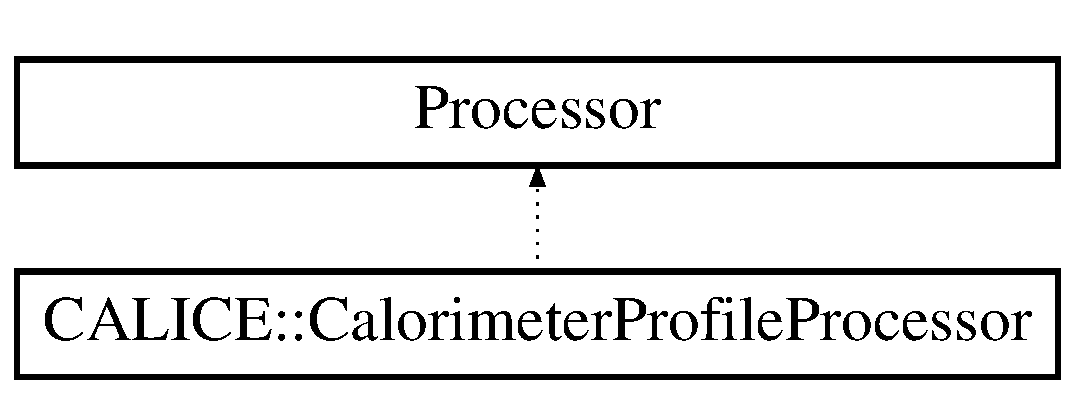
\includegraphics[height=2.000000cm]{classCALICE_1_1CalorimeterProfileProcessor}
\end{center}
\end{figure}
\subsection*{Public Member Functions}
\begin{DoxyCompactItemize}
\item 
virtual Processor $\ast$ {\bfseries new\-Processor} ()\label{classCALICE_1_1CalorimeterProfileProcessor_a9d924ca43abcbc887cba141381994aa2}

\item 
virtual void {\bfseries init} ()\label{classCALICE_1_1CalorimeterProfileProcessor_a82d456c3810e6142cd4b21fd0778245a}

\item 
virtual void {\bfseries process\-Event} (E\-V\-E\-N\-T\-::\-L\-C\-Event $\ast$evt)\label{classCALICE_1_1CalorimeterProfileProcessor_af622a71001b865c1df94369ee3116b84}

\item 
virtual void {\bfseries end} ()\label{classCALICE_1_1CalorimeterProfileProcessor_a9d5115ea8f88980722c655010eb2f271}

\end{DoxyCompactItemize}
\subsection*{Static Public Attributes}
\begin{DoxyCompactItemize}
\item 
static float {\bfseries \-\_\-debug\-S\-S\-Z}\label{classCALICE_1_1CalorimeterProfileProcessor_a329b77d1f703b4c44f68b7bb51fd919d}

\end{DoxyCompactItemize}
\subsection*{Protected Member Functions}
\begin{DoxyCompactItemize}
\item 
unsigned int {\bfseries get\-Index\-For\-Value} (const std\-::map$<$ float, unsigned int $>$ \&lookup, const float value) const \label{classCALICE_1_1CalorimeterProfileProcessor_a2e904d60f12b437d8d963251e2620de9}

\item 
void {\bfseries calculate\-Norm} (Float\-Vec \&r\-Norm, Float\-Vec \&l\-Norm, const std\-::map$<$ float, unsigned int $>$ \&r\-Index, const std\-::map$<$ float, unsigned int $>$ \&l\-Index, float x\-Offset=0, float y\-Offset=0, float z\-Offset=0)\label{classCALICE_1_1CalorimeterProfileProcessor_acdd500419ed31f6605a0fc2983ab6a08}

\item 
void {\bfseries calculate\-Norm} (Binned\-Vector$<$ float, Binned\-Vector$<$ float, float $>$ $>$ \&norm, Binned\-Vector$<$ float, Binned\-Vector$<$ float, float $>$ $>$ \&norm\-Low\-Bound, Binned\-Vector$<$ float, Binned\-Vector$<$ float, float $>$ $>$ \&norm\-High\-Bound, Binned\-Vector$<$ float, float $>$ \&r\-Norm, Binned\-Vector$<$ float, float $>$ \&l\-Norm, const float x\-Offset=0, const float y\-Offset=0, const float z\-Offset=0, const float low\-Bound\-Offset=0, const float high\-Bound\-Offset=0, bool calculate\-Bounds=false)\label{classCALICE_1_1CalorimeterProfileProcessor_a5efb4ffaaaa2532f72e3fd4170c32e57}

\item 
void {\bfseries fill\-Linear\-Float\-Vec} (const Binned\-Vector$<$ float, Binned\-Vector$<$ float, float $>$ $>$ \&input, Float\-Vec \&output) const \label{classCALICE_1_1CalorimeterProfileProcessor_afead74966f6ed0eeedbfcf82f2576742}

\item 
void {\bfseries fill\-Linear\-Center\-Float\-Vec} (const Binned\-Vector$<$ float, Binned\-Vector$<$ float, float $>$ $>$ \&input, Float\-Vec \&output\-\_\-center1, Float\-Vec \&output\-\_\-center2) const \label{classCALICE_1_1CalorimeterProfileProcessor_a938047f4934d3127e5381eefe63bdd92}

\end{DoxyCompactItemize}
\subsection*{Protected Attributes}
\begin{DoxyCompactItemize}
\item 
const Mapper $\ast$ {\bfseries \-\_\-mapper}\label{classCALICE_1_1CalorimeterProfileProcessor_a180872f0576cba660651644d8afd3c70}

\item 
Mapped\-Container$<$ {\bf Virtual\-Cells} $>$ $\ast$ {\bfseries \-\_\-virtual\-Cells}\label{classCALICE_1_1CalorimeterProfileProcessor_ae4628e74d54c7e3a4c9f0f8153641893}

\item 
Mapped\-Container\\*
$<$ Cell\-Description $>$ $\ast$ {\bfseries \-\_\-cell\-Descriptions}\label{classCALICE_1_1CalorimeterProfileProcessor_adac04f1d0b6c152dd47b33850c7e2897}

\end{DoxyCompactItemize}


\subsection{Detailed Description}
Processor to generate 3\-D shower profiles and to calculate the correct normalization.

\begin{DoxyAuthor}{Author}
B. Lutz 
\end{DoxyAuthor}
\begin{DoxyDate}{Date}
2010 
\end{DoxyDate}


The documentation for this class was generated from the following files\-:\begin{DoxyCompactItemize}
\item 
/nfs/dust/ilc/user/marquezh/\-Calice\-Soft\-\_\-w\-\_\-\-I\-L\-C\-Soft\-\_\-v02-\/03-\/02/calice\-\_\-analysis/addon\-Procs/include/Calorimeter\-Profile\-Processor.\-hh\item 
/nfs/dust/ilc/user/marquezh/\-Calice\-Soft\-\_\-w\-\_\-\-I\-L\-C\-Soft\-\_\-v02-\/03-\/02/calice\-\_\-analysis/addon\-Procs/src/Calorimeter\-Profile\-Processor.\-cc\end{DoxyCompactItemize}

\section{C\-Hit Class Reference}
\label{classCHit}\index{C\-Hit@{C\-Hit}}


{\ttfamily \#include $<$C\-A\-L\-I\-C\-E\-Overlay\-Preparation.\-hh$>$}

\subsection*{Public Member Functions}
\begin{DoxyCompactItemize}
\item 
{\bf C\-Hit} ()
\item 
{\bf $\sim$\-C\-Hit} ()
\item 
{\bf C\-Hit} ()
\item 
{\bf $\sim$\-C\-Hit} ()
\item 
{\bf C\-Hit} ()
\item 
{\bf $\sim$\-C\-Hit} ()
\end{DoxyCompactItemize}
\subsection*{Public Attributes}
\begin{DoxyCompactItemize}
\item 
bool {\bfseries tr}\label{classCHit_a7d49db2e8e443fb2d4dd8367bb7b113a}

\item 
bool {\bf b}
\item 
unsigned {\bf l}
\item 
float {\bf x}
\item 
float {\bf y}
\item 
float {\bf z}
\item 
float {\bf w}
\item 
float {\bf r}
\item 
Calorimeter\-Hit $\ast$ {\bf hit\-\_\-addr}
\item 
int {\bfseries l}\label{classCHit_a4938dfeea38c213d593cfb06e832d2d8}

\item 
float {\bf e}
\item 
float {\bf c}
\item 
int {\bf n1}
\item 
int {\bf n2}
\item 
int {\bf n3}
\item 
int {\bf nc}
\item 
int {\bf cell\-I\-D}
\end{DoxyCompactItemize}


\subsection{Detailed Description}
Auxiliary class to keep hit data 

\subsection{Constructor \& Destructor Documentation}
\index{C\-Hit@{C\-Hit}!C\-Hit@{C\-Hit}}
\index{C\-Hit@{C\-Hit}!CHit@{C\-Hit}}
\subsubsection[{C\-Hit}]{\setlength{\rightskip}{0pt plus 5cm}C\-Hit\-::\-C\-Hit (
\begin{DoxyParamCaption}
{}
\end{DoxyParamCaption}
)\hspace{0.3cm}{\ttfamily [inline]}}\label{classCHit_ad45ffd18358154f04797423e113c483b}
Constructor with member initialization \index{C\-Hit@{C\-Hit}!$\sim$\-C\-Hit@{$\sim$\-C\-Hit}}
\index{$\sim$\-C\-Hit@{$\sim$\-C\-Hit}!CHit@{C\-Hit}}
\subsubsection[{$\sim$\-C\-Hit}]{\setlength{\rightskip}{0pt plus 5cm}C\-Hit\-::$\sim$\-C\-Hit (
\begin{DoxyParamCaption}
{}
\end{DoxyParamCaption}
)\hspace{0.3cm}{\ttfamily [inline]}}\label{classCHit_aa46da91dc8cee6f79cc547802c49309c}
Default destructor \index{C\-Hit@{C\-Hit}!C\-Hit@{C\-Hit}}
\index{C\-Hit@{C\-Hit}!CHit@{C\-Hit}}
\subsubsection[{C\-Hit}]{\setlength{\rightskip}{0pt plus 5cm}C\-Hit\-::\-C\-Hit (
\begin{DoxyParamCaption}
{}
\end{DoxyParamCaption}
)\hspace{0.3cm}{\ttfamily [inline]}}\label{classCHit_ad45ffd18358154f04797423e113c483b}
Constructor with member initialization \index{C\-Hit@{C\-Hit}!$\sim$\-C\-Hit@{$\sim$\-C\-Hit}}
\index{$\sim$\-C\-Hit@{$\sim$\-C\-Hit}!CHit@{C\-Hit}}
\subsubsection[{$\sim$\-C\-Hit}]{\setlength{\rightskip}{0pt plus 5cm}C\-Hit\-::$\sim$\-C\-Hit (
\begin{DoxyParamCaption}
{}
\end{DoxyParamCaption}
)\hspace{0.3cm}{\ttfamily [inline]}}\label{classCHit_aa46da91dc8cee6f79cc547802c49309c}
Default destructor \index{C\-Hit@{C\-Hit}!C\-Hit@{C\-Hit}}
\index{C\-Hit@{C\-Hit}!CHit@{C\-Hit}}
\subsubsection[{C\-Hit}]{\setlength{\rightskip}{0pt plus 5cm}C\-Hit\-::\-C\-Hit (
\begin{DoxyParamCaption}
{}
\end{DoxyParamCaption}
)\hspace{0.3cm}{\ttfamily [inline]}}\label{classCHit_ad45ffd18358154f04797423e113c483b}
Constructor with member initialization \index{C\-Hit@{C\-Hit}!$\sim$\-C\-Hit@{$\sim$\-C\-Hit}}
\index{$\sim$\-C\-Hit@{$\sim$\-C\-Hit}!CHit@{C\-Hit}}
\subsubsection[{$\sim$\-C\-Hit}]{\setlength{\rightskip}{0pt plus 5cm}C\-Hit\-::$\sim$\-C\-Hit (
\begin{DoxyParamCaption}
{}
\end{DoxyParamCaption}
)\hspace{0.3cm}{\ttfamily [inline]}}\label{classCHit_aa46da91dc8cee6f79cc547802c49309c}
Default destructor 

\subsection{Member Data Documentation}
\index{C\-Hit@{C\-Hit}!b@{b}}
\index{b@{b}!CHit@{C\-Hit}}
\subsubsection[{b}]{\setlength{\rightskip}{0pt plus 5cm}bool C\-Hit\-::b}\label{classCHit_ac0a535a68f797bcd8b7226b10bcc6bc4}
true if belongs to track 

Referenced by C\-A\-L\-I\-C\-E\-Overlay\-Preparation\-::\-Find\-Track().

\index{C\-Hit@{C\-Hit}!c@{c}}
\index{c@{c}!CHit@{C\-Hit}}
\subsubsection[{c}]{\setlength{\rightskip}{0pt plus 5cm}float C\-Hit\-::c}\label{classCHit_a501007bdab32d174e272c37f2093fb7d}
Criteria for distance between neighbour hits \index{C\-Hit@{C\-Hit}!cell\-I\-D@{cell\-I\-D}}
\index{cell\-I\-D@{cell\-I\-D}!CHit@{C\-Hit}}
\subsubsection[{cell\-I\-D}]{\setlength{\rightskip}{0pt plus 5cm}int C\-Hit\-::cell\-I\-D}\label{classCHit_aeb31765ace5ca5ced6be5e56f806151f}
Cell size in mm \index{C\-Hit@{C\-Hit}!e@{e}}
\index{e@{e}!CHit@{C\-Hit}}
\subsubsection[{e}]{\setlength{\rightskip}{0pt plus 5cm}float C\-Hit\-::e}\label{classCHit_a350b70c6610b2a393237a14ee2f51310}
z coordinate of hit \index{C\-Hit@{C\-Hit}!hit\-\_\-addr@{hit\-\_\-addr}}
\index{hit\-\_\-addr@{hit\-\_\-addr}!CHit@{C\-Hit}}
\subsubsection[{hit\-\_\-addr}]{\setlength{\rightskip}{0pt plus 5cm}Calorimeter\-Hit$\ast$ C\-Hit\-::hit\-\_\-addr}\label{classCHit_ade131a1914418c0c30817fe19c02a885}
Criteria for distance between neighbour hits \index{C\-Hit@{C\-Hit}!l@{l}}
\index{l@{l}!CHit@{C\-Hit}}
\subsubsection[{l}]{\setlength{\rightskip}{0pt plus 5cm}unsigned C\-Hit\-::l}\label{classCHit_ae0fd15bed570010ba641d99302254a8c}
true if boundary cell 

Referenced by C\-A\-L\-I\-C\-E\-Overlay\-Preparation\-::\-Find\-Track(), and Find\-Start\-And\-Primary\-Track\-::get\-Number\-Of\-Neighbors().

\index{C\-Hit@{C\-Hit}!n1@{n1}}
\index{n1@{n1}!CHit@{C\-Hit}}
\subsubsection[{n1}]{\setlength{\rightskip}{0pt plus 5cm}int C\-Hit\-::n1}\label{classCHit_a50ee336cf5b7ab5da592ad67fd14882a}
Cell size in mm for track error estimate \index{C\-Hit@{C\-Hit}!n2@{n2}}
\index{n2@{n2}!CHit@{C\-Hit}}
\subsubsection[{n2}]{\setlength{\rightskip}{0pt plus 5cm}int C\-Hit\-::n2}\label{classCHit_a3cf1c537b50b1d4ca36bf733cd5e9371}
Number of neighbors in the same layer \index{C\-Hit@{C\-Hit}!n3@{n3}}
\index{n3@{n3}!CHit@{C\-Hit}}
\subsubsection[{n3}]{\setlength{\rightskip}{0pt plus 5cm}int C\-Hit\-::n3}\label{classCHit_a8c2cc381f1da1ad36df39800d13f5be0}
Number of neighbors in the same and previous layers \index{C\-Hit@{C\-Hit}!nc@{nc}}
\index{nc@{nc}!CHit@{C\-Hit}}
\subsubsection[{nc}]{\setlength{\rightskip}{0pt plus 5cm}int C\-Hit\-::nc}\label{classCHit_a8002afb784c7f3be853bedfe66524d94}
Number of neighbors around the hit \index{C\-Hit@{C\-Hit}!r@{r}}
\index{r@{r}!CHit@{C\-Hit}}
\subsubsection[{r}]{\setlength{\rightskip}{0pt plus 5cm}float C\-Hit\-::r}\label{classCHit_ac1bc0f62968053da2b6e42de30757397}
Weight for cell

Hit energy in M\-I\-P

Hit energy in M\-I\-Ps 

Referenced by Find\-Start\-And\-Primary\-Track\-::\-Find\-Track(), C\-A\-L\-I\-C\-E\-Overlay\-Preparation\-::\-Find\-Track(), and Find\-Start\-And\-Primary\-Track\-::get\-Number\-Of\-Neighbors().

\index{C\-Hit@{C\-Hit}!w@{w}}
\index{w@{w}!CHit@{C\-Hit}}
\subsubsection[{w}]{\setlength{\rightskip}{0pt plus 5cm}float C\-Hit\-::w}\label{classCHit_af6ca2e2627dfdada60123b07d995f979}
z coordinate of hit \index{C\-Hit@{C\-Hit}!x@{x}}
\index{x@{x}!CHit@{C\-Hit}}
\subsubsection[{x}]{\setlength{\rightskip}{0pt plus 5cm}float C\-Hit\-::x}\label{classCHit_a2d75c2ec6af4d1974d54dc7c95bb3769}
Layer number 

Referenced by C\-A\-L\-I\-C\-E\-Overlay\-Preparation\-::dist\-X\-Y(), Find\-Start\-And\-Primary\-Track\-::\-Find\-Track(), C\-A\-L\-I\-C\-E\-Overlay\-Preparation\-::\-Find\-Track(), and Find\-Start\-And\-Primary\-Track\-::get\-Number\-Of\-Neighbors().

\index{C\-Hit@{C\-Hit}!y@{y}}
\index{y@{y}!CHit@{C\-Hit}}
\subsubsection[{y}]{\setlength{\rightskip}{0pt plus 5cm}float C\-Hit\-::y}\label{classCHit_a9ae960cc5bb59e64f41814c05501067f}
x coordinate of hit 

Referenced by C\-A\-L\-I\-C\-E\-Overlay\-Preparation\-::dist\-X\-Y(), Find\-Start\-And\-Primary\-Track\-::\-Find\-Track(), C\-A\-L\-I\-C\-E\-Overlay\-Preparation\-::\-Find\-Track(), and Find\-Start\-And\-Primary\-Track\-::get\-Number\-Of\-Neighbors().

\index{C\-Hit@{C\-Hit}!z@{z}}
\index{z@{z}!CHit@{C\-Hit}}
\subsubsection[{z}]{\setlength{\rightskip}{0pt plus 5cm}float C\-Hit\-::z}\label{classCHit_ab1d439b8468fc38824edd2242475458e}
y coordinate of hit 

Referenced by C\-A\-L\-I\-C\-E\-Overlay\-Preparation\-::\-Find\-Track().



The documentation for this class was generated from the following files\-:\begin{DoxyCompactItemize}
\item 
/nfs/dust/ilc/user/marquezh/\-Calice\-Soft\-\_\-w\-\_\-\-I\-L\-C\-Soft\-\_\-v02-\/03-\/02/calice\-\_\-analysis/addon\-Procs/include/C\-A\-L\-I\-C\-E\-Overlay\-Preparation.\-hh\item 
/nfs/dust/ilc/user/marquezh/\-Calice\-Soft\-\_\-w\-\_\-\-I\-L\-C\-Soft\-\_\-v02-\/03-\/02/calice\-\_\-analysis/addon\-Procs/include/Find\-Start\-And\-Primary\-Track.\-h\item 
/nfs/dust/ilc/user/marquezh/\-Calice\-Soft\-\_\-w\-\_\-\-I\-L\-C\-Soft\-\_\-v02-\/03-\/02/calice\-\_\-analysis/addon\-Procs/include/Primary\-Track\-Finder.\-hh\end{DoxyCompactItemize}

\section{C\-A\-L\-I\-C\-E\-:\-:C\-Hit Class Reference}
\label{classCALICE_1_1CHit}\index{C\-A\-L\-I\-C\-E\-::\-C\-Hit@{C\-A\-L\-I\-C\-E\-::\-C\-Hit}}


{\ttfamily \#include $<$Shower\-Start\-Finding\-Processor.\-hh$>$}

\subsection*{Public Member Functions}
\begin{DoxyCompactItemize}
\item 
{\bf C\-Hit} ()
\item 
{\bf $\sim$\-C\-Hit} ()
\end{DoxyCompactItemize}
\subsection*{Public Attributes}
\begin{DoxyCompactItemize}
\item 
int {\bfseries l}\label{classCALICE_1_1CHit_ae0fd15bed570010ba641d99302254a8c}

\item 
float {\bf x}
\item 
float {\bf y}
\item 
float {\bf z}
\item 
float {\bf e}
\item 
float {\bf r}
\item 
float {\bf c}
\item 
int {\bf n1}
\item 
int {\bf n2}
\item 
int {\bf n3}
\item 
int {\bf nc}
\end{DoxyCompactItemize}


\subsection{Detailed Description}
Auxiliary class to keep hit data 

\subsection{Constructor \& Destructor Documentation}
\index{C\-A\-L\-I\-C\-E\-::\-C\-Hit@{C\-A\-L\-I\-C\-E\-::\-C\-Hit}!C\-Hit@{C\-Hit}}
\index{C\-Hit@{C\-Hit}!CALICE::CHit@{C\-A\-L\-I\-C\-E\-::\-C\-Hit}}
\subsubsection[{C\-Hit}]{\setlength{\rightskip}{0pt plus 5cm}C\-A\-L\-I\-C\-E\-::\-C\-Hit\-::\-C\-Hit (
\begin{DoxyParamCaption}
{}
\end{DoxyParamCaption}
)\hspace{0.3cm}{\ttfamily [inline]}}\label{classCALICE_1_1CHit_a6622cd3ad6d204e6ca418819743ecd7d}
Constructor with member initialization \index{C\-A\-L\-I\-C\-E\-::\-C\-Hit@{C\-A\-L\-I\-C\-E\-::\-C\-Hit}!$\sim$\-C\-Hit@{$\sim$\-C\-Hit}}
\index{$\sim$\-C\-Hit@{$\sim$\-C\-Hit}!CALICE::CHit@{C\-A\-L\-I\-C\-E\-::\-C\-Hit}}
\subsubsection[{$\sim$\-C\-Hit}]{\setlength{\rightskip}{0pt plus 5cm}C\-A\-L\-I\-C\-E\-::\-C\-Hit\-::$\sim$\-C\-Hit (
\begin{DoxyParamCaption}
{}
\end{DoxyParamCaption}
)\hspace{0.3cm}{\ttfamily [inline]}}\label{classCALICE_1_1CHit_a525fa9fce2eb17ffbd40825c7dc8328f}
Default destructor 

\subsection{Member Data Documentation}
\index{C\-A\-L\-I\-C\-E\-::\-C\-Hit@{C\-A\-L\-I\-C\-E\-::\-C\-Hit}!c@{c}}
\index{c@{c}!CALICE::CHit@{C\-A\-L\-I\-C\-E\-::\-C\-Hit}}
\subsubsection[{c}]{\setlength{\rightskip}{0pt plus 5cm}float C\-Hit\-::c}\label{classCALICE_1_1CHit_a501007bdab32d174e272c37f2093fb7d}
Criteria for distance between neighbour hits 

Referenced by Primary\-Track\-Finder\-::process\-Event().

\index{C\-A\-L\-I\-C\-E\-::\-C\-Hit@{C\-A\-L\-I\-C\-E\-::\-C\-Hit}!e@{e}}
\index{e@{e}!CALICE::CHit@{C\-A\-L\-I\-C\-E\-::\-C\-Hit}}
\subsubsection[{e}]{\setlength{\rightskip}{0pt plus 5cm}float C\-Hit\-::e}\label{classCALICE_1_1CHit_a350b70c6610b2a393237a14ee2f51310}
z coordinate of hit 

Referenced by Primary\-Track\-Finder\-::process\-Event().

\index{C\-A\-L\-I\-C\-E\-::\-C\-Hit@{C\-A\-L\-I\-C\-E\-::\-C\-Hit}!n1@{n1}}
\index{n1@{n1}!CALICE::CHit@{C\-A\-L\-I\-C\-E\-::\-C\-Hit}}
\subsubsection[{n1}]{\setlength{\rightskip}{0pt plus 5cm}int C\-A\-L\-I\-C\-E\-::\-C\-Hit\-::n1}\label{classCALICE_1_1CHit_ac76e3d9bbfa459b7a49cd30cc09639d3}
Cell size in mm for track error estimate \index{C\-A\-L\-I\-C\-E\-::\-C\-Hit@{C\-A\-L\-I\-C\-E\-::\-C\-Hit}!n2@{n2}}
\index{n2@{n2}!CALICE::CHit@{C\-A\-L\-I\-C\-E\-::\-C\-Hit}}
\subsubsection[{n2}]{\setlength{\rightskip}{0pt plus 5cm}int C\-A\-L\-I\-C\-E\-::\-C\-Hit\-::n2}\label{classCALICE_1_1CHit_a7eb720820d3c5a6d73393f4f4dafd835}
Number of neighbors in the same layer \index{C\-A\-L\-I\-C\-E\-::\-C\-Hit@{C\-A\-L\-I\-C\-E\-::\-C\-Hit}!n3@{n3}}
\index{n3@{n3}!CALICE::CHit@{C\-A\-L\-I\-C\-E\-::\-C\-Hit}}
\subsubsection[{n3}]{\setlength{\rightskip}{0pt plus 5cm}int C\-A\-L\-I\-C\-E\-::\-C\-Hit\-::n3}\label{classCALICE_1_1CHit_a2c9c0d94bba38ddb42a2e5f7f209c125}
Number of neighbors in the same and previous layers \index{C\-A\-L\-I\-C\-E\-::\-C\-Hit@{C\-A\-L\-I\-C\-E\-::\-C\-Hit}!nc@{nc}}
\index{nc@{nc}!CALICE::CHit@{C\-A\-L\-I\-C\-E\-::\-C\-Hit}}
\subsubsection[{nc}]{\setlength{\rightskip}{0pt plus 5cm}int C\-A\-L\-I\-C\-E\-::\-C\-Hit\-::nc}\label{classCALICE_1_1CHit_aec2c8db262fd4081b45342f3825dc375}
Number of neighbors around the hit \index{C\-A\-L\-I\-C\-E\-::\-C\-Hit@{C\-A\-L\-I\-C\-E\-::\-C\-Hit}!r@{r}}
\index{r@{r}!CALICE::CHit@{C\-A\-L\-I\-C\-E\-::\-C\-Hit}}
\subsubsection[{r}]{\setlength{\rightskip}{0pt plus 5cm}float C\-Hit\-::r}\label{classCALICE_1_1CHit_ac1bc0f62968053da2b6e42de30757397}
Hit energy in M\-I\-P

Hit energy in M\-I\-Ps 

Referenced by Primary\-Track\-Finder\-::\-Find\-Track(), C\-A\-L\-I\-C\-E\-Overlay\-Preparation\-::process\-Event(), and Primary\-Track\-Finder\-::process\-Event().

\index{C\-A\-L\-I\-C\-E\-::\-C\-Hit@{C\-A\-L\-I\-C\-E\-::\-C\-Hit}!x@{x}}
\index{x@{x}!CALICE::CHit@{C\-A\-L\-I\-C\-E\-::\-C\-Hit}}
\subsubsection[{x}]{\setlength{\rightskip}{0pt plus 5cm}float C\-Hit\-::x}\label{classCALICE_1_1CHit_a2d75c2ec6af4d1974d54dc7c95bb3769}
Layer number 

Referenced by Primary\-Track\-Finder\-::dist\-X\-Y(), Primary\-Track\-Finder\-::\-Find\-Track(), C\-A\-L\-I\-C\-E\-Overlay\-Preparation\-::process\-Event(), and Primary\-Track\-Finder\-::process\-Event().

\index{C\-A\-L\-I\-C\-E\-::\-C\-Hit@{C\-A\-L\-I\-C\-E\-::\-C\-Hit}!y@{y}}
\index{y@{y}!CALICE::CHit@{C\-A\-L\-I\-C\-E\-::\-C\-Hit}}
\subsubsection[{y}]{\setlength{\rightskip}{0pt plus 5cm}float C\-Hit\-::y}\label{classCALICE_1_1CHit_a9ae960cc5bb59e64f41814c05501067f}
x coordinate of hit 

Referenced by Primary\-Track\-Finder\-::dist\-X\-Y(), Primary\-Track\-Finder\-::\-Find\-Track(), C\-A\-L\-I\-C\-E\-Overlay\-Preparation\-::process\-Event(), and Primary\-Track\-Finder\-::process\-Event().

\index{C\-A\-L\-I\-C\-E\-::\-C\-Hit@{C\-A\-L\-I\-C\-E\-::\-C\-Hit}!z@{z}}
\index{z@{z}!CALICE::CHit@{C\-A\-L\-I\-C\-E\-::\-C\-Hit}}
\subsubsection[{z}]{\setlength{\rightskip}{0pt plus 5cm}float C\-Hit\-::z}\label{classCALICE_1_1CHit_ab1d439b8468fc38824edd2242475458e}
y coordinate of hit 

Referenced by Primary\-Track\-Finder\-::\-Find\-Track(), C\-A\-L\-I\-C\-E\-Overlay\-Preparation\-::process\-Event(), and Primary\-Track\-Finder\-::process\-Event().



The documentation for this class was generated from the following files\-:\begin{DoxyCompactItemize}
\item 
/nfs/dust/ilc/user/marquezh/\-Calice\-Soft\-\_\-w\-\_\-\-I\-L\-C\-Soft\-\_\-v02-\/03-\/02/calice\-\_\-analysis/addon\-Procs/include/Shower\-Start\-Finding\-Processor.\-hh\item 
/nfs/dust/ilc/user/marquezh/\-Calice\-Soft\-\_\-w\-\_\-\-I\-L\-C\-Soft\-\_\-v02-\/03-\/02/calice\-\_\-analysis/addon\-Procs/include/Primary\-Track\-Finder.\-hh\end{DoxyCompactItemize}

\section{C\-Layer Class Reference}
\label{classCLayer}\index{C\-Layer@{C\-Layer}}


{\ttfamily \#include $<$C\-A\-L\-I\-C\-E\-Overlay\-Preparation.\-hh$>$}

\subsection*{Public Member Functions}
\begin{DoxyCompactItemize}
\item 
{\bf C\-Layer} ()
\item 
{\bf $\sim$\-C\-Layer} ()
\item 
{\bf C\-Layer} ()
\item 
{\bf $\sim$\-C\-Layer} ()
\item 
{\bf C\-Layer} ()
\item 
{\bf $\sim$\-C\-Layer} ()
\end{DoxyCompactItemize}
\subsection*{Public Attributes}
\begin{DoxyCompactItemize}
\item 
std\-::vector$<$ {\bf C\-Hit} $\ast$ $>$ {\bfseries vl}\label{classCLayer_a1f81b6426a1fd05d9ee9c08caf280105}

\item 
int {\bfseries nh}\label{classCLayer_a5ebf93c7468c15249c7d9ff37cc5c4fc}

\item 
float {\bf emip}
\item 
int {\bfseries max1}\label{classCLayer_a5eab519f92a0f426a3c9e9ed6e0f1793}

\item 
int {\bfseries max2}\label{classCLayer_a95819cdd5d6756c7430fcf1139bcd6ec}

\item 
int {\bfseries max3}\label{classCLayer_a1d2af7d79dbe1b745afeddb90df0d301}

\end{DoxyCompactItemize}


\subsection{Detailed Description}
Auxiliary class to keep layer data 

\subsection{Constructor \& Destructor Documentation}
\index{C\-Layer@{C\-Layer}!C\-Layer@{C\-Layer}}
\index{C\-Layer@{C\-Layer}!CLayer@{C\-Layer}}
\subsubsection[{C\-Layer}]{\setlength{\rightskip}{0pt plus 5cm}C\-Layer\-::\-C\-Layer (
\begin{DoxyParamCaption}
{}
\end{DoxyParamCaption}
)\hspace{0.3cm}{\ttfamily [inline]}}\label{classCLayer_a6156e0a33ab7511c751d8ddc8975c9a3}
Constructor with member initialization \index{C\-Layer@{C\-Layer}!$\sim$\-C\-Layer@{$\sim$\-C\-Layer}}
\index{$\sim$\-C\-Layer@{$\sim$\-C\-Layer}!CLayer@{C\-Layer}}
\subsubsection[{$\sim$\-C\-Layer}]{\setlength{\rightskip}{0pt plus 5cm}C\-Layer\-::$\sim$\-C\-Layer (
\begin{DoxyParamCaption}
{}
\end{DoxyParamCaption}
)\hspace{0.3cm}{\ttfamily [inline]}}\label{classCLayer_a78d56eb9fffa4188383cdc0ca91ee67c}
Destructor with vector cleaning \index{C\-Layer@{C\-Layer}!C\-Layer@{C\-Layer}}
\index{C\-Layer@{C\-Layer}!CLayer@{C\-Layer}}
\subsubsection[{C\-Layer}]{\setlength{\rightskip}{0pt plus 5cm}C\-Layer\-::\-C\-Layer (
\begin{DoxyParamCaption}
{}
\end{DoxyParamCaption}
)\hspace{0.3cm}{\ttfamily [inline]}}\label{classCLayer_a6156e0a33ab7511c751d8ddc8975c9a3}
Constructor with member initialization \index{C\-Layer@{C\-Layer}!$\sim$\-C\-Layer@{$\sim$\-C\-Layer}}
\index{$\sim$\-C\-Layer@{$\sim$\-C\-Layer}!CLayer@{C\-Layer}}
\subsubsection[{$\sim$\-C\-Layer}]{\setlength{\rightskip}{0pt plus 5cm}C\-Layer\-::$\sim$\-C\-Layer (
\begin{DoxyParamCaption}
{}
\end{DoxyParamCaption}
)\hspace{0.3cm}{\ttfamily [inline]}}\label{classCLayer_a78d56eb9fffa4188383cdc0ca91ee67c}
Destructor with vector cleaning \index{C\-Layer@{C\-Layer}!C\-Layer@{C\-Layer}}
\index{C\-Layer@{C\-Layer}!CLayer@{C\-Layer}}
\subsubsection[{C\-Layer}]{\setlength{\rightskip}{0pt plus 5cm}C\-Layer\-::\-C\-Layer (
\begin{DoxyParamCaption}
{}
\end{DoxyParamCaption}
)\hspace{0.3cm}{\ttfamily [inline]}}\label{classCLayer_a6156e0a33ab7511c751d8ddc8975c9a3}
Constructor with member initialization \index{C\-Layer@{C\-Layer}!$\sim$\-C\-Layer@{$\sim$\-C\-Layer}}
\index{$\sim$\-C\-Layer@{$\sim$\-C\-Layer}!CLayer@{C\-Layer}}
\subsubsection[{$\sim$\-C\-Layer}]{\setlength{\rightskip}{0pt plus 5cm}C\-Layer\-::$\sim$\-C\-Layer (
\begin{DoxyParamCaption}
{}
\end{DoxyParamCaption}
)\hspace{0.3cm}{\ttfamily [inline]}}\label{classCLayer_a78d56eb9fffa4188383cdc0ca91ee67c}
Destructor with vector cleaning 

\subsection{Member Data Documentation}
\index{C\-Layer@{C\-Layer}!emip@{emip}}
\index{emip@{emip}!CLayer@{C\-Layer}}
\subsubsection[{emip}]{\setlength{\rightskip}{0pt plus 5cm}float C\-Layer\-::emip}\label{classCLayer_a5895428daee78075e1db8ebaf99f0b40}
number of hits per layer 

The documentation for this class was generated from the following files\-:\begin{DoxyCompactItemize}
\item 
/nfs/dust/ilc/user/marquezh/\-Calice\-Soft\-\_\-w\-\_\-\-I\-L\-C\-Soft\-\_\-v02-\/03-\/02/calice\-\_\-analysis/addon\-Procs/include/C\-A\-L\-I\-C\-E\-Overlay\-Preparation.\-hh\item 
/nfs/dust/ilc/user/marquezh/\-Calice\-Soft\-\_\-w\-\_\-\-I\-L\-C\-Soft\-\_\-v02-\/03-\/02/calice\-\_\-analysis/addon\-Procs/include/Find\-Start\-And\-Primary\-Track.\-h\item 
/nfs/dust/ilc/user/marquezh/\-Calice\-Soft\-\_\-w\-\_\-\-I\-L\-C\-Soft\-\_\-v02-\/03-\/02/calice\-\_\-analysis/addon\-Procs/include/Primary\-Track\-Finder.\-hh\end{DoxyCompactItemize}

\section{C\-A\-L\-I\-C\-E\-:\-:C\-Layer Class Reference}
\label{classCALICE_1_1CLayer}\index{C\-A\-L\-I\-C\-E\-::\-C\-Layer@{C\-A\-L\-I\-C\-E\-::\-C\-Layer}}


{\ttfamily \#include $<$Shower\-Start\-Finding\-Processor.\-hh$>$}

\subsection*{Public Member Functions}
\begin{DoxyCompactItemize}
\item 
{\bf C\-Layer} ()
\item 
{\bf $\sim$\-C\-Layer} ()
\end{DoxyCompactItemize}
\subsection*{Public Attributes}
\begin{DoxyCompactItemize}
\item 
std\-::vector$<$ {\bf C\-Hit} $>$ {\bfseries vl}\label{classCALICE_1_1CLayer_a1f81b6426a1fd05d9ee9c08caf280105}

\item 
int {\bfseries nh}\label{classCALICE_1_1CLayer_a5ebf93c7468c15249c7d9ff37cc5c4fc}

\item 
int {\bfseries max1}\label{classCALICE_1_1CLayer_a3914d8312e88ba70a161c3814cfeb906}

\item 
int {\bfseries max2}\label{classCALICE_1_1CLayer_aed809eafdd95d60d31b290ce6b43b574}

\item 
int {\bfseries max3}\label{classCALICE_1_1CLayer_a1ac008439a68abd6b30193a504cff3eb}

\item 
float {\bf emip}
\end{DoxyCompactItemize}


\subsection{Detailed Description}
Auxiliary class to keep layer data 

\subsection{Constructor \& Destructor Documentation}
\index{C\-A\-L\-I\-C\-E\-::\-C\-Layer@{C\-A\-L\-I\-C\-E\-::\-C\-Layer}!C\-Layer@{C\-Layer}}
\index{C\-Layer@{C\-Layer}!CALICE::CLayer@{C\-A\-L\-I\-C\-E\-::\-C\-Layer}}
\subsubsection[{C\-Layer}]{\setlength{\rightskip}{0pt plus 5cm}C\-A\-L\-I\-C\-E\-::\-C\-Layer\-::\-C\-Layer (
\begin{DoxyParamCaption}
{}
\end{DoxyParamCaption}
)\hspace{0.3cm}{\ttfamily [inline]}}\label{classCALICE_1_1CLayer_a043958dccd397b7720ace08f35089545}
Constructor with member initialization \index{C\-A\-L\-I\-C\-E\-::\-C\-Layer@{C\-A\-L\-I\-C\-E\-::\-C\-Layer}!$\sim$\-C\-Layer@{$\sim$\-C\-Layer}}
\index{$\sim$\-C\-Layer@{$\sim$\-C\-Layer}!CALICE::CLayer@{C\-A\-L\-I\-C\-E\-::\-C\-Layer}}
\subsubsection[{$\sim$\-C\-Layer}]{\setlength{\rightskip}{0pt plus 5cm}C\-A\-L\-I\-C\-E\-::\-C\-Layer\-::$\sim$\-C\-Layer (
\begin{DoxyParamCaption}
{}
\end{DoxyParamCaption}
)\hspace{0.3cm}{\ttfamily [inline]}}\label{classCALICE_1_1CLayer_ad599b283110a908807014d18de05f43e}
Destructor with vector cleaning 

\subsection{Member Data Documentation}
\index{C\-A\-L\-I\-C\-E\-::\-C\-Layer@{C\-A\-L\-I\-C\-E\-::\-C\-Layer}!emip@{emip}}
\index{emip@{emip}!CALICE::CLayer@{C\-A\-L\-I\-C\-E\-::\-C\-Layer}}
\subsubsection[{emip}]{\setlength{\rightskip}{0pt plus 5cm}float C\-Layer\-::emip}\label{classCALICE_1_1CLayer_a5895428daee78075e1db8ebaf99f0b40}
number of hits per layer 

Referenced by C\-A\-L\-I\-C\-E\-Overlay\-Preparation\-::process\-Event(), and Primary\-Track\-Finder\-::process\-Event().



The documentation for this class was generated from the following files\-:\begin{DoxyCompactItemize}
\item 
/nfs/dust/ilc/user/marquezh/\-Calice\-Soft\-\_\-w\-\_\-\-I\-L\-C\-Soft\-\_\-v02-\/03-\/02/calice\-\_\-analysis/addon\-Procs/include/Shower\-Start\-Finding\-Processor.\-hh\item 
/nfs/dust/ilc/user/marquezh/\-Calice\-Soft\-\_\-w\-\_\-\-I\-L\-C\-Soft\-\_\-v02-\/03-\/02/calice\-\_\-analysis/addon\-Procs/include/Primary\-Track\-Finder.\-hh\end{DoxyCompactItemize}

\section{C\-A\-L\-I\-C\-E\-:\-:Cluster\-Counter Class Reference}
\label{classCALICE_1_1ClusterCounter}\index{C\-A\-L\-I\-C\-E\-::\-Cluster\-Counter@{C\-A\-L\-I\-C\-E\-::\-Cluster\-Counter}}


Processor finds detached hits in event and gives 2 collections\-: Detached hits and event w/o detached hits.  




{\ttfamily \#include $<$Cluster\-Counter.\-hh$>$}

Inheritance diagram for C\-A\-L\-I\-C\-E\-:\-:Cluster\-Counter\-:\begin{figure}[H]
\begin{center}
\leavevmode
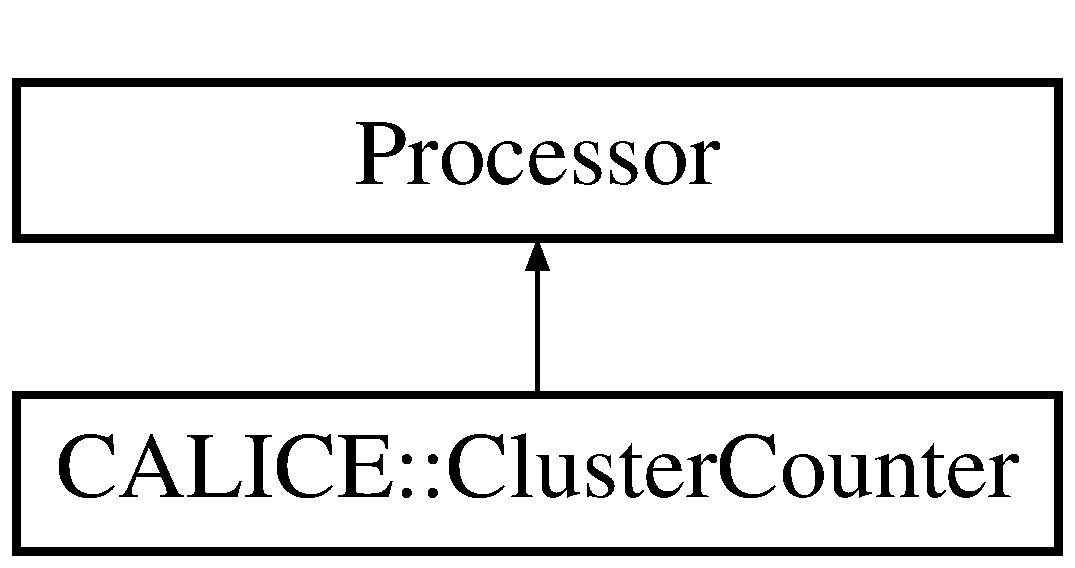
\includegraphics[height=2.000000cm]{classCALICE_1_1ClusterCounter}
\end{center}
\end{figure}
\subsection*{Public Member Functions}
\begin{DoxyCompactItemize}
\item 
virtual Processor $\ast$ {\bfseries new\-Processor} ()\label{classCALICE_1_1ClusterCounter_a2668a900c7d219826c97540555494823}

\item 
virtual void {\bfseries init} ()\label{classCALICE_1_1ClusterCounter_ac086e9b47fc8b7006479a762cd4e5205}

\item 
virtual void {\bfseries process\-Run\-Header} (L\-C\-Run\-Header $\ast$run)\label{classCALICE_1_1ClusterCounter_abc6eae26572f0a17304cf0a00b001bff}

\item 
virtual void {\bfseries process\-Event} (L\-C\-Event $\ast$evt)\label{classCALICE_1_1ClusterCounter_a6cc282e45a6f542eff586fd06b2d2d64}

\item 
virtual void {\bfseries check} (L\-C\-Event $\ast$evt)\label{classCALICE_1_1ClusterCounter_ad8bd193bd992b3a9c1081167fcebce5d}

\item 
virtual void {\bfseries end} ()\label{classCALICE_1_1ClusterCounter_a06075c6f41de3c59af21b9b26e6a0495}

\item 
virtual void {\bfseries print\-Parameters} ()\label{classCALICE_1_1ClusterCounter_a2369f1d140ba6e4686a949362e9b089c}

\item 
int {\bfseries group2\-D\-Cluster} (std\-::map$<$ std\-::array$<$ int, 2 $>$, Calorimeter\-Hit $\ast$ $>$ $\ast$\-\_\-hitmap, std\-::map$<$ std\-::array$<$ int, 2 $>$, Calorimeter\-Hit $\ast$ $>$ $\ast$\-\_\-seedmap)\label{classCALICE_1_1ClusterCounter_ad8594e8668b029a4c21728c48e197723}

\item 
int {\bfseries group3\-D\-Cluster} (std\-::map$<$ std\-::array$<$ int, 3 $>$, Calorimeter\-Hit $\ast$ $>$ $\ast$\-\_\-hitmap, std\-::map$<$ std\-::array$<$ int, 3 $>$, Calorimeter\-Hit $\ast$ $>$ $\ast$\-\_\-seedmap)\label{classCALICE_1_1ClusterCounter_a4fb3f495fbe2f049f1f8df9fc55d0c45}

\item 
Calorimeter\-Hit\-Vec {\bfseries get\-Neighbours3\-D} (std\-::array$<$ int, 3 $>$ \-\_\-seed, std\-::map$<$ std\-::array$<$ int, 3 $>$, Calorimeter\-Hit $\ast$ $>$ $\ast$\-\_\-map, int \-\_\-vol\-Half\-Size)\label{classCALICE_1_1ClusterCounter_a48b0dc007eea02357fa6254376e01a96}

\item 
void {\bfseries get\-Track\-Candidates} (std\-::map$<$ std\-::array$<$ int, 3 $>$, Calorimeter\-Hit $\ast$ $>$ $\ast$\-\_\-hitmap, std\-::map$<$ const float $\ast$, Calorimeter\-Hit $\ast$ $>$ $\ast$\-\_\-track\-Candidates, std\-::vector$<$ const float $\ast$ $>$ $\ast$\-\_\-candpositions)\label{classCALICE_1_1ClusterCounter_a0fbc91fa8970a74c23fc3d703fb215f7}

\item 
float {\bfseries get\-Dist\-Btw\-Positions} (const float $\ast$vec1, const float $\ast$vec2)\label{classCALICE_1_1ClusterCounter_a9bcc1daafc86819a4bacb2b0627fbb47}

\item 
float {\bfseries get\-Cos\-Btw\-Vectors} (const float $\ast$vec1, const float $\ast$vec2)\label{classCALICE_1_1ClusterCounter_a50fc201fdc59707bbf6bcfdc785c3a62}

\item 
float {\bfseries get\-Tracking\-Min\-Cos} (const float $\ast$\-\_\-checkvec)\label{classCALICE_1_1ClusterCounter_a166e683a158fe2ba8896a5365d8fb8ed}

\item 
int {\bfseries get\-Closest\-Neighbour} (const float $\ast$\-\_\-seed, std\-::vector$<$ const float $\ast$ $>$ $\ast$\-\_\-candpositions)\label{classCALICE_1_1ClusterCounter_aa026f09e7f6cb1e01920104e517dd7a7}

\item 
int {\bfseries group\-Track} (const float $\ast$seedpos, std\-::vector$<$ const float $\ast$ $>$ $\ast$\-\_\-candpositions, std\-::vector$<$ const float $\ast$ $>$ $\ast$\-\_\-trackvec, int \-\_\-maxgap, int startindex)\label{classCALICE_1_1ClusterCounter_a1934fceecaaaadf6afa948159e146a66}

\item 
std\-::array$<$ float, 3 $>$ {\bfseries get2\-D\-Cluster\-Co\-G} (std\-::map$<$ std\-::array$<$ int, 2 $>$, Calorimeter\-Hit $\ast$ $>$ $\ast$\-\_\-map)\label{classCALICE_1_1ClusterCounter_a5aeb7163d4ef3b7d6446fd333cfb0c0a}

\item 
void {\bfseries add2\-D\-Map\-To\-Cluster} (I\-M\-P\-L\-::\-Cluster\-Impl $\ast$\-\_\-cluster, std\-::map$<$ std\-::array$<$ int, 2 $>$, Calorimeter\-Hit $\ast$ $>$ $\ast$\-\_\-map)\label{classCALICE_1_1ClusterCounter_a73014ac09605de1878969ce20c04b725}

\item 
void {\bfseries add3\-D\-Map\-To\-Cluster} (I\-M\-P\-L\-::\-Cluster\-Impl $\ast$\-\_\-cluster, std\-::map$<$ std\-::array$<$ int, 3 $>$, Calorimeter\-Hit $\ast$ $>$ $\ast$\-\_\-map)\label{classCALICE_1_1ClusterCounter_a3a1f9e8010caabbd2aa65a60b91eb9e0}

\end{DoxyCompactItemize}
\subsection*{Static Public Member Functions}
\begin{DoxyCompactItemize}
\item 
static bool {\bfseries comparison} (const float $\ast$pos1, const float $\ast$pos2)\label{classCALICE_1_1ClusterCounter_a6eff0a034511d76aa5dde76768b03698}

\end{DoxyCompactItemize}
\subsection*{Protected Attributes}
\begin{DoxyCompactItemize}
\item 
std\-::string {\bfseries \-\_\-evt\-Var\-Col\-Name}\label{classCALICE_1_1ClusterCounter_a982f03b5d49994d25198f88f6ad0cdab}

\item 
std\-::string {\bfseries \-\_\-lay\-Var\-Col\-Name}\label{classCALICE_1_1ClusterCounter_a0bc5b4e964e43d7db247693efdd2ca66}

\item 
std\-::string {\bfseries \-\_\-layer2hit\-Relations\-Col\-Name}\label{classCALICE_1_1ClusterCounter_a32a906dfc1fc61780f63ff0ee99dcb62}

\item 
std\-::string {\bfseries \-\_\-hit2hit\-Var\-Relations\-Col\-Name}\label{classCALICE_1_1ClusterCounter_a48af01e6e60fad4b4e49b7a32922d5c8}

\item 
std\-::string {\bfseries \-\_\-2\-D\-Cluster\-Out\-Col\-Name}\label{classCALICE_1_1ClusterCounter_ada733e376dc13e11c75d7928b8afa4b4}

\item 
std\-::string {\bfseries \-\_\-3\-D\-Cluster\-Out\-Col\-Name}\label{classCALICE_1_1ClusterCounter_a94e01f495efc808b0b93ab15a3ecce1d}

\item 
std\-::string {\bfseries \-\_\-\-L2\-C\-Out\-Rel\-Col\-Name}\label{classCALICE_1_1ClusterCounter_adac38a6a8d9dd38e9a5b65f4d2f324b4}

\item 
bool {\bfseries \-\_\-write\-Root\-File}\label{classCALICE_1_1ClusterCounter_ac73b4352462fa9c65685758db2fc330d}

\item 
std\-::string {\bfseries \-\_\-\-Root\-Output}\label{classCALICE_1_1ClusterCounter_aaba2acfb9913b2a6a13891c59656053a}

\item 
int {\bfseries \-\_\-min\-Hitst\-In2\-D\-Cluster}\label{classCALICE_1_1ClusterCounter_afa8b19f9538e5f67619b6b2f9da26eef}

\item 
int {\bfseries \-\_\-min\-Hitst\-In3\-D\-Cluster}\label{classCALICE_1_1ClusterCounter_af26ed7b753085b8d18c291866a01641d}

\item 
int {\bfseries \-\_\-\-Kmax\-For3\-D\-Cluster}\label{classCALICE_1_1ClusterCounter_a34a45c42488d5fb2b42d064b1001896d}

\item 
int {\bfseries \-\_\-volume\-Tsize}\label{classCALICE_1_1ClusterCounter_a9d7ee1bd08670973f52411830c558b51}

\item 
int {\bfseries \-\_\-volume\-Lsize}\label{classCALICE_1_1ClusterCounter_a1d36c4726d82e0dcd6f62e565565f3a5}

\item 
bool {\bfseries \-\_\-filter\-Hits}\label{classCALICE_1_1ClusterCounter_a24eea26f3210c9e6b3d645c5da02094b}

\item 
std\-::array$<$ float, 3 $>$ {\bfseries Co\-G}\label{classCALICE_1_1ClusterCounter_a24adb4a8cb17221b9824af53e990c587}

\item 
int {\bfseries n2\-D\-Clusters}\label{classCALICE_1_1ClusterCounter_a5a60f78ab7d7420fb40ef88071d83685}

\item 
int {\bfseries n3\-D\-Clusters}\label{classCALICE_1_1ClusterCounter_a56495d0202d0c80204f07e092152b6a1}

\item 
int {\bf \-\_\-n\-Run}
\item 
int {\bf \-\_\-n\-Evt}
\item 
float {\bfseries cos\-To\-Beam} = -\/2.\label{classCALICE_1_1ClusterCounter_a52a7998cbc4329982ec23b26bdececcc}

\item 
std\-::array$<$ float, 3 $>$ {\bfseries trackdr}\label{classCALICE_1_1ClusterCounter_a7f6731c5a090d8460117a94e02c944f0}

\item 
std\-::array$<$ float, 3 $>$ {\bfseries mu}\label{classCALICE_1_1ClusterCounter_a873256023111e24ee3a5caee51e04b3f}

\item 
float {\bfseries w\-\_\-x}\label{classCALICE_1_1ClusterCounter_a51e43848f80981936b3a4140b2d6f001}

\item 
float {\bfseries w\-\_\-y}\label{classCALICE_1_1ClusterCounter_a197cfacf40a5cd66331d278237e0f396}

\item 
float {\bfseries denom\-\_\-w}\label{classCALICE_1_1ClusterCounter_af040902ac4a8a8c3b17e7a93708be566}

\item 
int {\bfseries n\-Track\-Hits}\label{classCALICE_1_1ClusterCounter_a9869b8046c512b783427a5bfe820b384}

\item 
int {\bfseries track\-Nr}\label{classCALICE_1_1ClusterCounter_a73fd682f635eb37e350ef447abaed972}

\item 
float {\bfseries tr\-Esum}\label{classCALICE_1_1ClusterCounter_a1a189518671f3d5b77cf08cf32ab18c0}

\item 
std\-::vector$<$ float $>$ {\bfseries hit\-Energies}\label{classCALICE_1_1ClusterCounter_ab1608ebe4c4b6e1d544f407c008cfcd0}

\end{DoxyCompactItemize}


\subsection{Detailed Description}
Processor finds detached hits in event and gives 2 collections\-: Detached hits and event w/o detached hits. 

\begin{DoxyAuthor}{Author}
{\tt vladimir.\-bocharnikov@desy.\-de} 
\end{DoxyAuthor}
\begin{DoxyVersion}{Version}
1.\-0 
\end{DoxyVersion}
\begin{DoxyDate}{Date}
December 2018 
\end{DoxyDate}


\subsection{Member Data Documentation}
\index{C\-A\-L\-I\-C\-E\-::\-Cluster\-Counter@{C\-A\-L\-I\-C\-E\-::\-Cluster\-Counter}!\-\_\-n\-Evt@{\-\_\-n\-Evt}}
\index{\-\_\-n\-Evt@{\-\_\-n\-Evt}!CALICE::ClusterCounter@{C\-A\-L\-I\-C\-E\-::\-Cluster\-Counter}}
\subsubsection[{\-\_\-n\-Evt}]{\setlength{\rightskip}{0pt plus 5cm}int C\-A\-L\-I\-C\-E\-::\-Cluster\-Counter\-::\-\_\-n\-Evt\hspace{0.3cm}{\ttfamily [protected]}}\label{classCALICE_1_1ClusterCounter_acd3e96d9b95b78f5902e484f20e2b9ab}
evt number \index{C\-A\-L\-I\-C\-E\-::\-Cluster\-Counter@{C\-A\-L\-I\-C\-E\-::\-Cluster\-Counter}!\-\_\-n\-Run@{\-\_\-n\-Run}}
\index{\-\_\-n\-Run@{\-\_\-n\-Run}!CALICE::ClusterCounter@{C\-A\-L\-I\-C\-E\-::\-Cluster\-Counter}}
\subsubsection[{\-\_\-n\-Run}]{\setlength{\rightskip}{0pt plus 5cm}int C\-A\-L\-I\-C\-E\-::\-Cluster\-Counter\-::\-\_\-n\-Run\hspace{0.3cm}{\ttfamily [protected]}}\label{classCALICE_1_1ClusterCounter_aa839b23c89bea85c92b3cf3bbf4dd89d}
run number 

The documentation for this class was generated from the following files\-:\begin{DoxyCompactItemize}
\item 
/nfs/dust/ilc/user/marquezh/\-Calice\-Soft\-\_\-w\-\_\-\-I\-L\-C\-Soft\-\_\-v02-\/03-\/02/calice\-\_\-analysis/addon\-Procs/include/Cluster\-Counter.\-hh\item 
/nfs/dust/ilc/user/marquezh/\-Calice\-Soft\-\_\-w\-\_\-\-I\-L\-C\-Soft\-\_\-v02-\/03-\/02/calice\-\_\-analysis/addon\-Procs/src/Cluster\-Counter.\-cc\end{DoxyCompactItemize}

\section{C\-A\-L\-I\-C\-E\-:\-:Cluster\-Pattern\-Processor Class Reference}
\label{classCALICE_1_1ClusterPatternProcessor}\index{C\-A\-L\-I\-C\-E\-::\-Cluster\-Pattern\-Processor@{C\-A\-L\-I\-C\-E\-::\-Cluster\-Pattern\-Processor}}


{\ttfamily \#include $<$Cluster\-Pattern\-Processor.\-hh$>$}

Inheritance diagram for C\-A\-L\-I\-C\-E\-:\-:Cluster\-Pattern\-Processor\-:\begin{figure}[H]
\begin{center}
\leavevmode
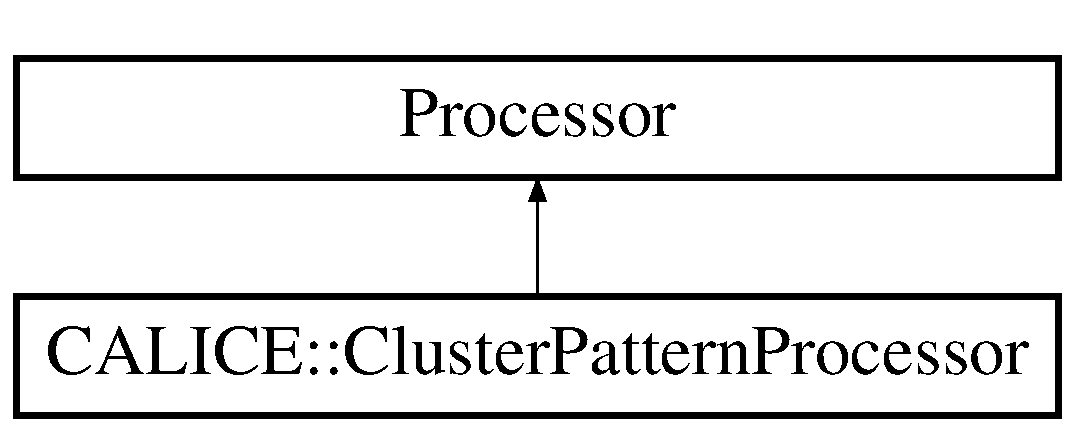
\includegraphics[height=2.000000cm]{classCALICE_1_1ClusterPatternProcessor}
\end{center}
\end{figure}
\subsection*{Public Member Functions}
\begin{DoxyCompactItemize}
\item 
virtual Processor $\ast$ {\bfseries new\-Processor} ()\label{classCALICE_1_1ClusterPatternProcessor_aee6d74ab69cf1a8b78964049490a2c49}

\item 
virtual void {\bfseries init} ()\label{classCALICE_1_1ClusterPatternProcessor_a0ae021ab872248ee9ec3b9804412addb}

\item 
virtual void {\bfseries process\-Run\-Header} (L\-C\-Run\-Header $\ast$run)\label{classCALICE_1_1ClusterPatternProcessor_a7149fcb85cff870aaa634b54a37a211a}

\item 
virtual void {\bfseries process\-Event} (L\-C\-Event $\ast$evt)\label{classCALICE_1_1ClusterPatternProcessor_ab3b03b66a70ade9ea67dfb43a5755ff1}

\item 
virtual void {\bfseries end} ()\label{classCALICE_1_1ClusterPatternProcessor_a68bf2e0dcd9cceafaf99a08fa48c8e90}

\end{DoxyCompactItemize}


\subsection{Detailed Description}
Processor which analyzes clusters (e.\-g. provided by the Shower\-Start\-Custer\-Processor) in an event to extract maximum energy and hits in a single cluster or the overlap of separate clusters.

\begin{DoxyAuthor}{Author}
{\tt nils.\-feege@desy.\-de} 
\end{DoxyAuthor}
\begin{DoxyDate}{Date}
April 2011 
\end{DoxyDate}


The documentation for this class was generated from the following files\-:\begin{DoxyCompactItemize}
\item 
/nfs/dust/ilc/user/marquezh/\-Calice\-Soft\-\_\-w\-\_\-\-I\-L\-C\-Soft\-\_\-v02-\/03-\/02/calice\-\_\-analysis/addon\-Procs/include/Cluster\-Pattern\-Processor.\-hh\item 
/nfs/dust/ilc/user/marquezh/\-Calice\-Soft\-\_\-w\-\_\-\-I\-L\-C\-Soft\-\_\-v02-\/03-\/02/calice\-\_\-analysis/addon\-Procs/src/Cluster\-Pattern\-Processor.\-cc\end{DoxyCompactItemize}

\section{C\-A\-L\-I\-C\-E\-:\-:Convert\-Ampl2\-Calo\-Hit\-Processor Class Reference}
\label{classCALICE_1_1ConvertAmpl2CaloHitProcessor}\index{C\-A\-L\-I\-C\-E\-::\-Convert\-Ampl2\-Calo\-Hit\-Processor@{C\-A\-L\-I\-C\-E\-::\-Convert\-Ampl2\-Calo\-Hit\-Processor}}


{\ttfamily \#include $<$Convert\-Ampl2\-Calo\-Hit\-Processor.\-hh$>$}

Inheritance diagram for C\-A\-L\-I\-C\-E\-:\-:Convert\-Ampl2\-Calo\-Hit\-Processor\-:\begin{figure}[H]
\begin{center}
\leavevmode
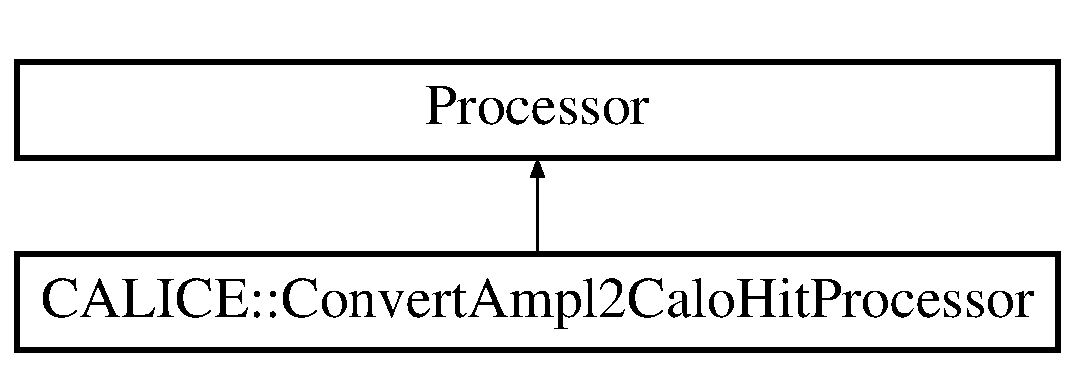
\includegraphics[height=2.000000cm]{classCALICE_1_1ConvertAmpl2CaloHitProcessor}
\end{center}
\end{figure}
\subsection*{Public Member Functions}
\begin{DoxyCompactItemize}
\item 
{\bf Convert\-Ampl2\-Calo\-Hit\-Processor} $\ast$ {\bf new\-Processor} ()
\item 
{\bf Convert\-Ampl2\-Calo\-Hit\-Processor} ()
\item 
{\bf $\sim$\-Convert\-Ampl2\-Calo\-Hit\-Processor} ()
\item 
virtual void {\bf init} ()
\item 
virtual void {\bf process\-Event} (L\-C\-Event $\ast$evt)
\item 
virtual void {\bf end} ()
\end{DoxyCompactItemize}
\subsection*{Protected Attributes}
\begin{DoxyCompactItemize}
\item 
std\-::string {\bf \-\_\-ahc\-Hit\-Col\-Name}
\item 
std\-::string {\bf \-\_\-ahc\-Ampl\-Col\-Name}
\item 
std\-::string {\bf \-\_\-hit\-Ampl\-Relation\-Col\-Name}
\item 
std\-::string {\bf \-\_\-ahc\-Hit\-Output\-V2\-Col\-Name}
\item 
std\-::string {\bf \-\_\-ampl\-Name}
\end{DoxyCompactItemize}


\subsection{Detailed Description}
Processor which converts an Ahc\-Amplitude\-Relation collection to a Calorimeter\-Hits collection.

\begin{DoxyAuthor}{Author}
{\tt nils.\-feege@desy.\-de} 
\end{DoxyAuthor}
\begin{DoxyDate}{Date}
January 2011 
\end{DoxyDate}


\subsection{Constructor \& Destructor Documentation}
\index{C\-A\-L\-I\-C\-E\-::\-Convert\-Ampl2\-Calo\-Hit\-Processor@{C\-A\-L\-I\-C\-E\-::\-Convert\-Ampl2\-Calo\-Hit\-Processor}!Convert\-Ampl2\-Calo\-Hit\-Processor@{Convert\-Ampl2\-Calo\-Hit\-Processor}}
\index{Convert\-Ampl2\-Calo\-Hit\-Processor@{Convert\-Ampl2\-Calo\-Hit\-Processor}!CALICE::ConvertAmpl2CaloHitProcessor@{C\-A\-L\-I\-C\-E\-::\-Convert\-Ampl2\-Calo\-Hit\-Processor}}
\subsubsection[{Convert\-Ampl2\-Calo\-Hit\-Processor}]{\setlength{\rightskip}{0pt plus 5cm}C\-A\-L\-I\-C\-E\-::\-Convert\-Ampl2\-Calo\-Hit\-Processor\-::\-Convert\-Ampl2\-Calo\-Hit\-Processor (
\begin{DoxyParamCaption}
{}
\end{DoxyParamCaption}
)}\label{classCALICE_1_1ConvertAmpl2CaloHitProcessor_a3ece83f39a4b688cc612b6dc82b59c84}
Default constructor 

References \-\_\-ahc\-Ampl\-Col\-Name, \-\_\-ahc\-Hit\-Col\-Name, \-\_\-ahc\-Hit\-Output\-V2\-Col\-Name, \-\_\-ampl\-Name, and \-\_\-hit\-Ampl\-Relation\-Col\-Name.



Referenced by new\-Processor().

\index{C\-A\-L\-I\-C\-E\-::\-Convert\-Ampl2\-Calo\-Hit\-Processor@{C\-A\-L\-I\-C\-E\-::\-Convert\-Ampl2\-Calo\-Hit\-Processor}!$\sim$\-Convert\-Ampl2\-Calo\-Hit\-Processor@{$\sim$\-Convert\-Ampl2\-Calo\-Hit\-Processor}}
\index{$\sim$\-Convert\-Ampl2\-Calo\-Hit\-Processor@{$\sim$\-Convert\-Ampl2\-Calo\-Hit\-Processor}!CALICE::ConvertAmpl2CaloHitProcessor@{C\-A\-L\-I\-C\-E\-::\-Convert\-Ampl2\-Calo\-Hit\-Processor}}
\subsubsection[{$\sim$\-Convert\-Ampl2\-Calo\-Hit\-Processor}]{\setlength{\rightskip}{0pt plus 5cm}C\-A\-L\-I\-C\-E\-::\-Convert\-Ampl2\-Calo\-Hit\-Processor\-::$\sim$\-Convert\-Ampl2\-Calo\-Hit\-Processor (
\begin{DoxyParamCaption}
{}
\end{DoxyParamCaption}
)\hspace{0.3cm}{\ttfamily [inline]}}\label{classCALICE_1_1ConvertAmpl2CaloHitProcessor_aa65c16e3769a83f7dda850a536124d34}
Destructor 

\subsection{Member Function Documentation}
\index{C\-A\-L\-I\-C\-E\-::\-Convert\-Ampl2\-Calo\-Hit\-Processor@{C\-A\-L\-I\-C\-E\-::\-Convert\-Ampl2\-Calo\-Hit\-Processor}!end@{end}}
\index{end@{end}!CALICE::ConvertAmpl2CaloHitProcessor@{C\-A\-L\-I\-C\-E\-::\-Convert\-Ampl2\-Calo\-Hit\-Processor}}
\subsubsection[{end}]{\setlength{\rightskip}{0pt plus 5cm}void C\-A\-L\-I\-C\-E\-::\-Convert\-Ampl2\-Calo\-Hit\-Processor\-::end (
\begin{DoxyParamCaption}
{}
\end{DoxyParamCaption}
)\hspace{0.3cm}{\ttfamily [virtual]}}\label{classCALICE_1_1ConvertAmpl2CaloHitProcessor_ad1a50d41b2d3bf3fda6bbde40b7b4354}
Function called after all events have been processed, for cleanup \index{C\-A\-L\-I\-C\-E\-::\-Convert\-Ampl2\-Calo\-Hit\-Processor@{C\-A\-L\-I\-C\-E\-::\-Convert\-Ampl2\-Calo\-Hit\-Processor}!init@{init}}
\index{init@{init}!CALICE::ConvertAmpl2CaloHitProcessor@{C\-A\-L\-I\-C\-E\-::\-Convert\-Ampl2\-Calo\-Hit\-Processor}}
\subsubsection[{init}]{\setlength{\rightskip}{0pt plus 5cm}void C\-A\-L\-I\-C\-E\-::\-Convert\-Ampl2\-Calo\-Hit\-Processor\-::init (
\begin{DoxyParamCaption}
{}
\end{DoxyParamCaption}
)\hspace{0.3cm}{\ttfamily [virtual]}}\label{classCALICE_1_1ConvertAmpl2CaloHitProcessor_a561f09c937c62f066fe965dcd4358a34}
Initialise variables, if needed \index{C\-A\-L\-I\-C\-E\-::\-Convert\-Ampl2\-Calo\-Hit\-Processor@{C\-A\-L\-I\-C\-E\-::\-Convert\-Ampl2\-Calo\-Hit\-Processor}!new\-Processor@{new\-Processor}}
\index{new\-Processor@{new\-Processor}!CALICE::ConvertAmpl2CaloHitProcessor@{C\-A\-L\-I\-C\-E\-::\-Convert\-Ampl2\-Calo\-Hit\-Processor}}
\subsubsection[{new\-Processor}]{\setlength{\rightskip}{0pt plus 5cm}{\bf Convert\-Ampl2\-Calo\-Hit\-Processor}$\ast$ C\-A\-L\-I\-C\-E\-::\-Convert\-Ampl2\-Calo\-Hit\-Processor\-::new\-Processor (
\begin{DoxyParamCaption}
{}
\end{DoxyParamCaption}
)\hspace{0.3cm}{\ttfamily [inline]}}\label{classCALICE_1_1ConvertAmpl2CaloHitProcessor_a3e276bde455ac2354058d9b8fe80d3b9}
Return a new instance of this processor 

References Convert\-Ampl2\-Calo\-Hit\-Processor().

\index{C\-A\-L\-I\-C\-E\-::\-Convert\-Ampl2\-Calo\-Hit\-Processor@{C\-A\-L\-I\-C\-E\-::\-Convert\-Ampl2\-Calo\-Hit\-Processor}!process\-Event@{process\-Event}}
\index{process\-Event@{process\-Event}!CALICE::ConvertAmpl2CaloHitProcessor@{C\-A\-L\-I\-C\-E\-::\-Convert\-Ampl2\-Calo\-Hit\-Processor}}
\subsubsection[{process\-Event}]{\setlength{\rightskip}{0pt plus 5cm}void C\-A\-L\-I\-C\-E\-::\-Convert\-Ampl2\-Calo\-Hit\-Processor\-::process\-Event (
\begin{DoxyParamCaption}
\item[{L\-C\-Event $\ast$}]{evt}
\end{DoxyParamCaption}
)\hspace{0.3cm}{\ttfamily [virtual]}}\label{classCALICE_1_1ConvertAmpl2CaloHitProcessor_a44987f31c02f5fae87c55b1ef4bac7a0}
Process event (the working horse) 
\begin{DoxyParams}{Parameters}
{\em evt} & event to be processed \\
\hline
\end{DoxyParams}


References \-\_\-ahc\-Hit\-Col\-Name, \-\_\-ahc\-Hit\-Output\-V2\-Col\-Name, \-\_\-ampl\-Name, and \-\_\-hit\-Ampl\-Relation\-Col\-Name.



\subsection{Member Data Documentation}
\index{C\-A\-L\-I\-C\-E\-::\-Convert\-Ampl2\-Calo\-Hit\-Processor@{C\-A\-L\-I\-C\-E\-::\-Convert\-Ampl2\-Calo\-Hit\-Processor}!\-\_\-ahc\-Ampl\-Col\-Name@{\-\_\-ahc\-Ampl\-Col\-Name}}
\index{\-\_\-ahc\-Ampl\-Col\-Name@{\-\_\-ahc\-Ampl\-Col\-Name}!CALICE::ConvertAmpl2CaloHitProcessor@{C\-A\-L\-I\-C\-E\-::\-Convert\-Ampl2\-Calo\-Hit\-Processor}}
\subsubsection[{\-\_\-ahc\-Ampl\-Col\-Name}]{\setlength{\rightskip}{0pt plus 5cm}std\-::string C\-A\-L\-I\-C\-E\-::\-Convert\-Ampl2\-Calo\-Hit\-Processor\-::\-\_\-ahc\-Ampl\-Col\-Name\hspace{0.3cm}{\ttfamily [protected]}}\label{classCALICE_1_1ConvertAmpl2CaloHitProcessor_a7bd1b45af294e4ecf31f566847dd061f}
name of the input A\-H\-C amplitude collection 

Referenced by Convert\-Ampl2\-Calo\-Hit\-Processor().

\index{C\-A\-L\-I\-C\-E\-::\-Convert\-Ampl2\-Calo\-Hit\-Processor@{C\-A\-L\-I\-C\-E\-::\-Convert\-Ampl2\-Calo\-Hit\-Processor}!\-\_\-ahc\-Hit\-Col\-Name@{\-\_\-ahc\-Hit\-Col\-Name}}
\index{\-\_\-ahc\-Hit\-Col\-Name@{\-\_\-ahc\-Hit\-Col\-Name}!CALICE::ConvertAmpl2CaloHitProcessor@{C\-A\-L\-I\-C\-E\-::\-Convert\-Ampl2\-Calo\-Hit\-Processor}}
\subsubsection[{\-\_\-ahc\-Hit\-Col\-Name}]{\setlength{\rightskip}{0pt plus 5cm}std\-::string C\-A\-L\-I\-C\-E\-::\-Convert\-Ampl2\-Calo\-Hit\-Processor\-::\-\_\-ahc\-Hit\-Col\-Name\hspace{0.3cm}{\ttfamily [protected]}}\label{classCALICE_1_1ConvertAmpl2CaloHitProcessor_aea4cd71d349f6520f903b1fd6edb1aac}
name of the input A\-H\-C hit collection 

Referenced by Convert\-Ampl2\-Calo\-Hit\-Processor(), and process\-Event().

\index{C\-A\-L\-I\-C\-E\-::\-Convert\-Ampl2\-Calo\-Hit\-Processor@{C\-A\-L\-I\-C\-E\-::\-Convert\-Ampl2\-Calo\-Hit\-Processor}!\-\_\-ahc\-Hit\-Output\-V2\-Col\-Name@{\-\_\-ahc\-Hit\-Output\-V2\-Col\-Name}}
\index{\-\_\-ahc\-Hit\-Output\-V2\-Col\-Name@{\-\_\-ahc\-Hit\-Output\-V2\-Col\-Name}!CALICE::ConvertAmpl2CaloHitProcessor@{C\-A\-L\-I\-C\-E\-::\-Convert\-Ampl2\-Calo\-Hit\-Processor}}
\subsubsection[{\-\_\-ahc\-Hit\-Output\-V2\-Col\-Name}]{\setlength{\rightskip}{0pt plus 5cm}std\-::string C\-A\-L\-I\-C\-E\-::\-Convert\-Ampl2\-Calo\-Hit\-Processor\-::\-\_\-ahc\-Hit\-Output\-V2\-Col\-Name\hspace{0.3cm}{\ttfamily [protected]}}\label{classCALICE_1_1ConvertAmpl2CaloHitProcessor_afbacc464c40229ac6c825dd7d9ac3a4c}
name of the output A\-H\-C hit version 2 collection 

Referenced by Convert\-Ampl2\-Calo\-Hit\-Processor(), and process\-Event().

\index{C\-A\-L\-I\-C\-E\-::\-Convert\-Ampl2\-Calo\-Hit\-Processor@{C\-A\-L\-I\-C\-E\-::\-Convert\-Ampl2\-Calo\-Hit\-Processor}!\-\_\-ampl\-Name@{\-\_\-ampl\-Name}}
\index{\-\_\-ampl\-Name@{\-\_\-ampl\-Name}!CALICE::ConvertAmpl2CaloHitProcessor@{C\-A\-L\-I\-C\-E\-::\-Convert\-Ampl2\-Calo\-Hit\-Processor}}
\subsubsection[{\-\_\-ampl\-Name}]{\setlength{\rightskip}{0pt plus 5cm}std\-::string C\-A\-L\-I\-C\-E\-::\-Convert\-Ampl2\-Calo\-Hit\-Processor\-::\-\_\-ampl\-Name\hspace{0.3cm}{\ttfamily [protected]}}\label{classCALICE_1_1ConvertAmpl2CaloHitProcessor_a1cf4049cb77b69803d3826cc9d6fa9a7}
name of the new amplitude used for the output hit collection 

Referenced by Convert\-Ampl2\-Calo\-Hit\-Processor(), and process\-Event().

\index{C\-A\-L\-I\-C\-E\-::\-Convert\-Ampl2\-Calo\-Hit\-Processor@{C\-A\-L\-I\-C\-E\-::\-Convert\-Ampl2\-Calo\-Hit\-Processor}!\-\_\-hit\-Ampl\-Relation\-Col\-Name@{\-\_\-hit\-Ampl\-Relation\-Col\-Name}}
\index{\-\_\-hit\-Ampl\-Relation\-Col\-Name@{\-\_\-hit\-Ampl\-Relation\-Col\-Name}!CALICE::ConvertAmpl2CaloHitProcessor@{C\-A\-L\-I\-C\-E\-::\-Convert\-Ampl2\-Calo\-Hit\-Processor}}
\subsubsection[{\-\_\-hit\-Ampl\-Relation\-Col\-Name}]{\setlength{\rightskip}{0pt plus 5cm}std\-::string C\-A\-L\-I\-C\-E\-::\-Convert\-Ampl2\-Calo\-Hit\-Processor\-::\-\_\-hit\-Ampl\-Relation\-Col\-Name\hspace{0.3cm}{\ttfamily [protected]}}\label{classCALICE_1_1ConvertAmpl2CaloHitProcessor_ad89c705437cb9ed98577893592e5d63a}
name of the L\-C\-Relation collection between Calorimeter\-Hit and Ahc\-Amplitude 

Referenced by Convert\-Ampl2\-Calo\-Hit\-Processor(), and process\-Event().



The documentation for this class was generated from the following files\-:\begin{DoxyCompactItemize}
\item 
/nfs/dust/ilc/user/marquezh/\-Calice\-Soft\-\_\-w\-\_\-\-I\-L\-C\-Soft\-\_\-v02-\/03-\/02/calice\-\_\-analysis/addon\-Procs/include/Convert\-Ampl2\-Calo\-Hit\-Processor.\-hh\item 
/nfs/dust/ilc/user/marquezh/\-Calice\-Soft\-\_\-w\-\_\-\-I\-L\-C\-Soft\-\_\-v02-\/03-\/02/calice\-\_\-analysis/addon\-Procs/src/Convert\-Ampl2\-Calo\-Hit\-Processor.\-cc\end{DoxyCompactItemize}

\section{C\-A\-L\-I\-C\-E\-:\-:Convert\-Position\-To\-Layer Class Reference}
\label{classCALICE_1_1ConvertPositionToLayer}\index{C\-A\-L\-I\-C\-E\-::\-Convert\-Position\-To\-Layer@{C\-A\-L\-I\-C\-E\-::\-Convert\-Position\-To\-Layer}}


Processor for converting a position Float\-Vec parameter to the number of the closest layer.  




{\ttfamily \#include $<$Convert\-Position\-To\-Layer.\-hh$>$}

Inheritance diagram for C\-A\-L\-I\-C\-E\-:\-:Convert\-Position\-To\-Layer\-:\begin{figure}[H]
\begin{center}
\leavevmode
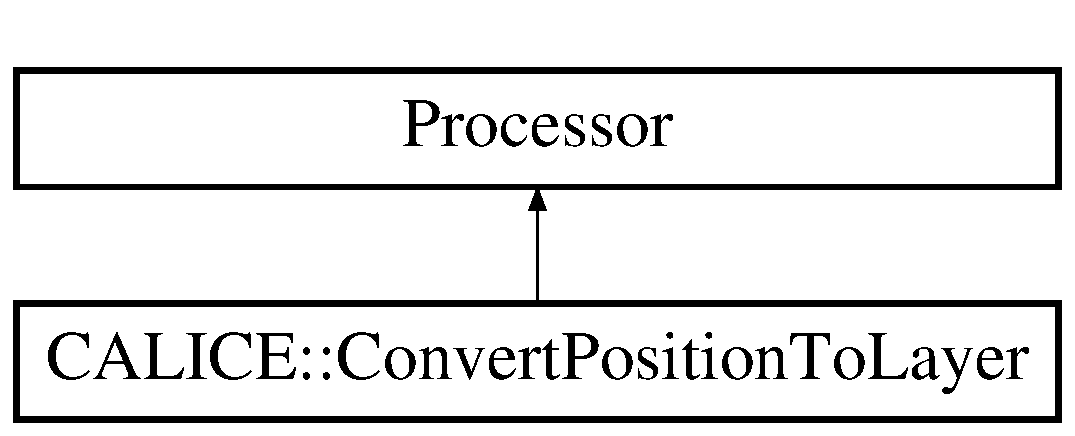
\includegraphics[height=2.000000cm]{classCALICE_1_1ConvertPositionToLayer}
\end{center}
\end{figure}
\subsection*{Public Member Functions}
\begin{DoxyCompactItemize}
\item 
virtual Processor $\ast$ {\bfseries new\-Processor} ()\label{classCALICE_1_1ConvertPositionToLayer_a19c62a73c4ea6636b31e98780dfe4dbd}

\item 
virtual void {\bf init} ()
\item 
virtual void {\bf process\-Run\-Header} (L\-C\-Run\-Header $\ast$run)
\item 
virtual void {\bf process\-Event} (L\-C\-Event $\ast$evt)
\item 
virtual void {\bfseries check} (L\-C\-Event $\ast$evt)\label{classCALICE_1_1ConvertPositionToLayer_a87177a62a9c55eda1209410efd4b7481}

\item 
virtual void {\bf end} ()
\end{DoxyCompactItemize}
\subsection*{Protected Attributes}
\begin{DoxyCompactItemize}
\item 
std\-::string {\bfseries \-\_\-par\-Name\-In}\label{classCALICE_1_1ConvertPositionToLayer_ab5771bf5dceebc05cf241c2f1268f6b3}

\item 
std\-::string {\bfseries \-\_\-cell\-I\-D\-Encoding}\label{classCALICE_1_1ConvertPositionToLayer_a373ae619279f0f1eb0c9277c236fe028}

\item 
std\-::string {\bfseries \-\_\-mapping\-Processor\-Name}\label{classCALICE_1_1ConvertPositionToLayer_a91aff57d115d8a16f06ac8f7939af5c7}

\item 
std\-::string {\bfseries \-\_\-cell\-Description\-Processor\-Name}\label{classCALICE_1_1ConvertPositionToLayer_af49914c248523c4a8d520fd238324202}

\item 
int {\bfseries \-\_\-n\-Run}\label{classCALICE_1_1ConvertPositionToLayer_ad2fd992c4000098077792de317bbb5b1}

\item 
int {\bfseries \-\_\-n\-Evt}\label{classCALICE_1_1ConvertPositionToLayer_ac4ce3ac8a9bfe3bf2d22e0e293346c3f}

\item 
const C\-A\-L\-I\-C\-E\-::\-Mapper $\ast$ {\bfseries \-\_\-mapper}\label{classCALICE_1_1ConvertPositionToLayer_a17d64aa238473785c0df64b0a5614b6f}

\item 
unsigned int {\bfseries \-\_\-mapper\-Version}\label{classCALICE_1_1ConvertPositionToLayer_a3195a7855b8d5baffdfc3cde745630e5}

\item 
C\-A\-L\-I\-C\-E\-::\-Mapped\-Container\\*
$<$ C\-A\-L\-I\-C\-E\-::\-Cell\-Description $>$ $\ast$ {\bfseries \-\_\-cell\-Descriptions}\label{classCALICE_1_1ConvertPositionToLayer_a3abd6f7b37da7cd4f13e9207c13c9fd7}

\end{DoxyCompactItemize}


\subsection{Detailed Description}
Processor for converting a position Float\-Vec parameter to the number of the closest layer. 

\begin{DoxyAuthor}{Author}
N. Feege, University of Hamburg 
\end{DoxyAuthor}
\begin{DoxyDate}{Date}
Dec 2010 
\end{DoxyDate}


\subsection{Member Function Documentation}
\index{C\-A\-L\-I\-C\-E\-::\-Convert\-Position\-To\-Layer@{C\-A\-L\-I\-C\-E\-::\-Convert\-Position\-To\-Layer}!end@{end}}
\index{end@{end}!CALICE::ConvertPositionToLayer@{C\-A\-L\-I\-C\-E\-::\-Convert\-Position\-To\-Layer}}
\subsubsection[{end}]{\setlength{\rightskip}{0pt plus 5cm}void C\-A\-L\-I\-C\-E\-::\-Convert\-Position\-To\-Layer\-::end (
\begin{DoxyParamCaption}
{}
\end{DoxyParamCaption}
)\hspace{0.3cm}{\ttfamily [virtual]}}\label{classCALICE_1_1ConvertPositionToLayer_ac66a2dbdfd05395fa80d848f1910d24a}
Called after data processing for clean up. \index{C\-A\-L\-I\-C\-E\-::\-Convert\-Position\-To\-Layer@{C\-A\-L\-I\-C\-E\-::\-Convert\-Position\-To\-Layer}!init@{init}}
\index{init@{init}!CALICE::ConvertPositionToLayer@{C\-A\-L\-I\-C\-E\-::\-Convert\-Position\-To\-Layer}}
\subsubsection[{init}]{\setlength{\rightskip}{0pt plus 5cm}void C\-A\-L\-I\-C\-E\-::\-Convert\-Position\-To\-Layer\-::init (
\begin{DoxyParamCaption}
{}
\end{DoxyParamCaption}
)\hspace{0.3cm}{\ttfamily [virtual]}}\label{classCALICE_1_1ConvertPositionToLayer_a526400d819dea92c0cd829c08aff0054}
Called at the begin of the job before anything is read. Use to initialize the processor, e.\-g. book histograms. \index{C\-A\-L\-I\-C\-E\-::\-Convert\-Position\-To\-Layer@{C\-A\-L\-I\-C\-E\-::\-Convert\-Position\-To\-Layer}!process\-Event@{process\-Event}}
\index{process\-Event@{process\-Event}!CALICE::ConvertPositionToLayer@{C\-A\-L\-I\-C\-E\-::\-Convert\-Position\-To\-Layer}}
\subsubsection[{process\-Event}]{\setlength{\rightskip}{0pt plus 5cm}void C\-A\-L\-I\-C\-E\-::\-Convert\-Position\-To\-Layer\-::process\-Event (
\begin{DoxyParamCaption}
\item[{L\-C\-Event $\ast$}]{evt}
\end{DoxyParamCaption}
)\hspace{0.3cm}{\ttfamily [virtual]}}\label{classCALICE_1_1ConvertPositionToLayer_af739937006d956958e4340d0a3e104e3}
Called for every event -\/ the working horse. \index{C\-A\-L\-I\-C\-E\-::\-Convert\-Position\-To\-Layer@{C\-A\-L\-I\-C\-E\-::\-Convert\-Position\-To\-Layer}!process\-Run\-Header@{process\-Run\-Header}}
\index{process\-Run\-Header@{process\-Run\-Header}!CALICE::ConvertPositionToLayer@{C\-A\-L\-I\-C\-E\-::\-Convert\-Position\-To\-Layer}}
\subsubsection[{process\-Run\-Header}]{\setlength{\rightskip}{0pt plus 5cm}void C\-A\-L\-I\-C\-E\-::\-Convert\-Position\-To\-Layer\-::process\-Run\-Header (
\begin{DoxyParamCaption}
\item[{L\-C\-Run\-Header $\ast$}]{run}
\end{DoxyParamCaption}
)\hspace{0.3cm}{\ttfamily [virtual]}}\label{classCALICE_1_1ConvertPositionToLayer_ac8e3edf234bfb030a487be80f5c11892}
Called for every run. 

The documentation for this class was generated from the following files\-:\begin{DoxyCompactItemize}
\item 
/nfs/dust/ilc/user/marquezh/\-Calice\-Soft\-\_\-w\-\_\-\-I\-L\-C\-Soft\-\_\-v02-\/03-\/02/calice\-\_\-analysis/addon\-Procs/include/Convert\-Position\-To\-Layer.\-hh\item 
/nfs/dust/ilc/user/marquezh/\-Calice\-Soft\-\_\-w\-\_\-\-I\-L\-C\-Soft\-\_\-v02-\/03-\/02/calice\-\_\-analysis/addon\-Procs/src/Convert\-Position\-To\-Layer.\-cc\end{DoxyCompactItemize}

\section{C\-A\-L\-I\-C\-E\-:\-:D\-E\-H\-Event\-Display\-Processor Class Reference}
\label{classCALICE_1_1DEHEventDisplayProcessor}\index{C\-A\-L\-I\-C\-E\-::\-D\-E\-H\-Event\-Display\-Processor@{C\-A\-L\-I\-C\-E\-::\-D\-E\-H\-Event\-Display\-Processor}}


This is a Marlin processor for displaying events with C\-E\-D.  




{\ttfamily \#include $<$D\-E\-H\-Event\-Display\-Processor.\-hh$>$}

Inheritance diagram for C\-A\-L\-I\-C\-E\-:\-:D\-E\-H\-Event\-Display\-Processor\-:\begin{figure}[H]
\begin{center}
\leavevmode
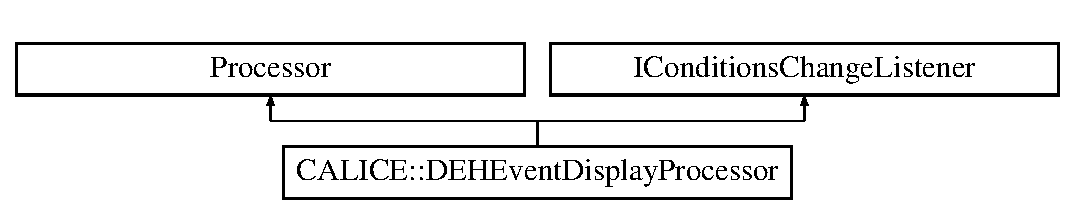
\includegraphics[height=2.000000cm]{classCALICE_1_1DEHEventDisplayProcessor}
\end{center}
\end{figure}
\subsection*{Public Member Functions}
\begin{DoxyCompactItemize}
\item 
virtual Processor $\ast$ {\bfseries new\-Processor} ()\label{classCALICE_1_1DEHEventDisplayProcessor_a7bcbd39aa9d9ea57a7c1175969cca469}

\item 
virtual void {\bf init} ()
\item 
virtual void {\bf process\-Run\-Header} (L\-C\-Run\-Header $\ast$run)
\item 
virtual void {\bf process\-Event} (L\-C\-Event $\ast$evt)
\item 
virtual void {\bfseries check} (L\-C\-Event $\ast$evt)\label{classCALICE_1_1DEHEventDisplayProcessor_ae42ba19ef5fa0c4c62bde36f8a40210e}

\item 
virtual void {\bf end} ()
\item 
virtual void {\bfseries conditions\-Changed} (L\-C\-Collection $\ast$col)\label{classCALICE_1_1DEHEventDisplayProcessor_a8230ef1e48e8ef2c3dae20ed3d009f70}

\end{DoxyCompactItemize}
\subsection*{Protected Member Functions}
\begin{DoxyCompactItemize}
\item 
void {\bfseries choose\-Color\-And\-Layer} (const float var, unsigned int \&color, unsigned int \&layer, const bool is\-Time) const \label{classCALICE_1_1DEHEventDisplayProcessor_ac3a2cd66ec049d6dc9d1be7e4829ff97}

\item 
void {\bfseries draw\-Cell} (const C\-A\-L\-I\-C\-E\-::\-Cell\-Description $\ast$description, const unsigned int color, const unsigned int layer, const bool solid=true) const \label{classCALICE_1_1DEHEventDisplayProcessor_a50d7ae11587eaffc110175b5a2ae36b0}

\item 
void {\bfseries draw\-Cell2} (const C\-A\-L\-I\-C\-E\-::\-Cell\-Description $\ast$description, const unsigned int color, const unsigned int layer, const bool solid=true) const \label{classCALICE_1_1DEHEventDisplayProcessor_a2ec7b70ac889295aebe4252d893ca824}

\item 
void {\bfseries draw\-Hit} (const Calorimeter\-Hit $\ast$hit, const unsigned int color, const unsigned int layer) const \label{classCALICE_1_1DEHEventDisplayProcessor_ad392af5f327b5237ea67100bb7ae4c08}

\item 
void {\bfseries draw\-Start\-Layer} (int st, int M\-C\-\_\-st, int n\-Layers)\label{classCALICE_1_1DEHEventDisplayProcessor_ab865f57c34a1678a857a1f0b51e0e856}

\item 
bool {\bfseries is\-T0event} (L\-C\-Event $\ast$evt)\label{classCALICE_1_1DEHEventDisplayProcessor_a90277317c86ea420cdb2134226911ce2}

\item 
void {\bfseries draw\-Module} (int module\-\_\-type, double module\-\_\-center\-\_\-pos[3])\label{classCALICE_1_1DEHEventDisplayProcessor_a418386562f71c855a4fb0e63043dc5b0}

\item 
void {\bfseries draw\-Detector\-D\-E\-H} ()\label{classCALICE_1_1DEHEventDisplayProcessor_a597cfeb5229cfecdace31719ac7ab310}

\item 
void {\bfseries draw\-Event} (L\-C\-Collection $\ast$col)\label{classCALICE_1_1DEHEventDisplayProcessor_afd7f3ba14295ded2c618286f193f7935}

\item 
void {\bfseries draw\-Track} (L\-C\-Collection $\ast$col\-D\-W\-C)\label{classCALICE_1_1DEHEventDisplayProcessor_a457826afbf89e0097d088a47a5001122}

\end{DoxyCompactItemize}
\subsection*{Protected Attributes}
\begin{DoxyCompactItemize}
\item 
std\-::string {\bfseries \-\_\-col\-Name\-Ecal}\label{classCALICE_1_1DEHEventDisplayProcessor_a3289554659565ea59fab72086c5f7262}

\item 
std\-::string {\bfseries \-\_\-col\-Name\-Hcal}\label{classCALICE_1_1DEHEventDisplayProcessor_ae846c99fb4cfdaa66b66aa97fa08c441}

\item 
std\-::string {\bfseries \-\_\-col\-Name\-T\-C}\label{classCALICE_1_1DEHEventDisplayProcessor_ac3c36067a80e698cc6c57afd080fd774}

\item 
std\-::string {\bfseries \-\_\-col\-Name\-P\-S}\label{classCALICE_1_1DEHEventDisplayProcessor_adde9c073c88b2153ea5c105d8d341cb4}

\item 
std\-::string {\bfseries \-\_\-evt\-Var\-Col\-Name}\label{classCALICE_1_1DEHEventDisplayProcessor_a2e9f79846f709e25102187f5add83f5c}

\item 
std\-::string {\bfseries \-\_\-mapping\-Processor\-Name}\label{classCALICE_1_1DEHEventDisplayProcessor_aa1134a1ba0a930a7d9cf30f3166b21ae}

\item 
std\-::string {\bfseries \-\_\-cell\-Neighbours\-Processor\-Name}\label{classCALICE_1_1DEHEventDisplayProcessor_a45d08934c78bcb6b60f083cb91ca3699}

\item 
std\-::string {\bfseries \-\_\-cell\-Description\-Processor\-Name}\label{classCALICE_1_1DEHEventDisplayProcessor_a82c342737a9c59f3a889b0b32f2526a0}

\item 
std\-::string {\bf \-\_\-calib\-Processor\-Name}
\item 
std\-::string {\bfseries \-\_\-col\-Name\-Module\-Location}\label{classCALICE_1_1DEHEventDisplayProcessor_a03c7635b25f7787509292ddb0bc1c8fb}

\item 
bool {\bfseries \-\_\-module\-Location\-Changed}\label{classCALICE_1_1DEHEventDisplayProcessor_a97ab7f75fca58beab3dba3fbd1c40e40}

\item 
L\-C\-Collection $\ast$ {\bfseries \-\_\-col\-Module\-Location}\label{classCALICE_1_1DEHEventDisplayProcessor_aad3d88faa8b335f007179424e6c32892}

\item 
int {\bfseries \-\_\-wait\-For\-Key\-Pressed}\label{classCALICE_1_1DEHEventDisplayProcessor_ac23ee5414f7dfee1ac7a1a964a47e43d}

\item 
int {\bfseries \-\_\-draw}\label{classCALICE_1_1DEHEventDisplayProcessor_a73cedbcb76c8729dc2505dae7ea59781}

\item 
bool {\bfseries \-\_\-drawst}\label{classCALICE_1_1DEHEventDisplayProcessor_abb9bbd4c81c80014a427d159f06ab665}

\item 
int {\bfseries \-\_\-append\-To\-Existing\-C\-E\-D}\label{classCALICE_1_1DEHEventDisplayProcessor_a065675fc34402136abccacad2972fafa}

\item 
int {\bfseries \-\_\-port\-C\-E\-D}\label{classCALICE_1_1DEHEventDisplayProcessor_a180e0db34944e7b648bf660ee8d22bef}

\item 
bool {\bfseries \-\_\-do\-T0selection}\label{classCALICE_1_1DEHEventDisplayProcessor_a4e6b1ea5cef1ae4b6fbbd6b5416f6676}

\item 
bool {\bfseries \-\_\-save\-Log\-File}\label{classCALICE_1_1DEHEventDisplayProcessor_a8212d153ec6124ecbb29e05cc606dbe2}

\item 
int {\bfseries \-\_\-n\-T0s}\label{classCALICE_1_1DEHEventDisplayProcessor_a70a1f949c685f2c50c96ba162b4ab4a9}

\item 
int {\bfseries \-\_\-min\-N\-Hits}\label{classCALICE_1_1DEHEventDisplayProcessor_a9b9bed227a184719f6bc60d5007ab93d}

\item 
bool {\bfseries \-\_\-use\-\_\-time}\label{classCALICE_1_1DEHEventDisplayProcessor_ac478a3791616d44bb295d4a362a40f34}

\item 
int {\bfseries \-\_\-n\-Hits}\label{classCALICE_1_1DEHEventDisplayProcessor_ad9e07963ec64eb57545a0d2dbc2287e1}

\item 
int {\bfseries st}\label{classCALICE_1_1DEHEventDisplayProcessor_ad0b8b037b954683d444d7380ca7e0687}

\item 
int {\bfseries M\-C\-\_\-st}\label{classCALICE_1_1DEHEventDisplayProcessor_aba9ff8366393bf786c70b55a30b3a712}

\item 
int {\bfseries n\-Layers}\label{classCALICE_1_1DEHEventDisplayProcessor_afb9e4ce990b1aa46d41b9ddbd0ac4334}

\item 
std\-::vector$<$ std\-::string $>$ {\bfseries \-\_\-input\-Collection\-Names}\label{classCALICE_1_1DEHEventDisplayProcessor_a876ee13be41fde039c633d0b95b125b1}

\item 
std\-::string {\bfseries \-\_\-input\-Collection\-Name\-D\-W\-C}\label{classCALICE_1_1DEHEventDisplayProcessor_ab7f37d394e605192982299404553f089}

\item 
int {\bfseries \-\_\-track\-Draw}\label{classCALICE_1_1DEHEventDisplayProcessor_a5d37f26bf9fc8b1797c48d0e966fb795}

\item 
float {\bfseries \-\_\-module\-Max\-Z}\label{classCALICE_1_1DEHEventDisplayProcessor_aef3e2dcfec8f27efa8d8dab1fa07b5e2}

\item 
std\-::vector$<$ float $>$ {\bfseries \-\_\-track\-Offsets}\label{classCALICE_1_1DEHEventDisplayProcessor_a2821ed36ee9cbac64300ae42cd74b1b6}

\item 
String\-Vec {\bf \-\_\-\-T0\-Vector}
\item 
std\-::map$<$ int, std\-::vector\\*
$<$ std\-::pair$<$ int, int $>$ $>$ $>$ {\bf \-\_\-map\-T0s}
\item 
int {\bfseries \-\_\-n\-Run}\label{classCALICE_1_1DEHEventDisplayProcessor_ae190101e05f623eb201892e6e2b4a295}

\item 
int {\bfseries \-\_\-n\-Evt}\label{classCALICE_1_1DEHEventDisplayProcessor_af03c1e1ba652a7a52abf66b7a0cb0b11}

\item 
const C\-A\-L\-I\-C\-E\-::\-Ahc2\-Mapper $\ast$ {\bfseries \-\_\-mapper}\label{classCALICE_1_1DEHEventDisplayProcessor_ab73ecddabf9a09c62b9467945bc37b87}

\item 
unsigned int {\bfseries \-\_\-mapper\-Version}\label{classCALICE_1_1DEHEventDisplayProcessor_a953b0f6038741b2623287ea486c67880}

\item 
C\-A\-L\-I\-C\-E\-::\-Mapped\-Container\\*
$<$ C\-A\-L\-I\-C\-E\-::\-Cell\-Description $>$ $\ast$ {\bfseries \-\_\-cell\-Descriptions}\label{classCALICE_1_1DEHEventDisplayProcessor_a5633bc4a5de6184583c15e6dfa3be325}

\item 
C\-A\-L\-I\-C\-E\-::\-Mapped\-Container\\*
$<$ C\-A\-L\-I\-C\-E\-::\-Cell\-Neighbours $>$ $\ast$ {\bfseries \-\_\-cell\-Neighbours}\label{classCALICE_1_1DEHEventDisplayProcessor_aaeb9c54cefb3a9cdfb34272aecce6112}

\item 
C\-A\-L\-I\-C\-E\-::\-Mapped\-Container\\*
$<$ C\-A\-L\-I\-C\-E\-::\-Ahc2\-Calibrations $>$ $\ast$ {\bf \-\_\-calib\-Container}
\end{DoxyCompactItemize}


\subsection{Detailed Description}
This is a Marlin processor for displaying events with C\-E\-D. 

If you want to display events with C\-E\-D, you need to start the display ({\ttfamily glced}) before running Marlin.

Mouse commands that can be used within C\-E\-D\-:


\begin{DoxyItemize}
\item {\ttfamily  left + move } -\/$>$ rotate view
\item {\ttfamily  right + move down/up } -\/$>$ zoom view in/out
\item {\ttfamily  center + move } -\/$>$ shift view
\item {\ttfamily  wheel } -\/$>$ shift view along z-\/axis
\end{DoxyItemize}

Keyboard commands that can be used within C\-E\-D\-:


\begin{DoxyItemize}
\item {\ttfamily  b } -\/$>$ toggle background color
\item {\ttfamily  r } -\/$>$ got to default angular view
\item {\ttfamily  s } -\/$>$ got to default side view
\item {\ttfamily  f } -\/$>$ got to default front view
\item {\ttfamily  v } -\/$>$ switch on/off fisheye view
\item {\ttfamily  0 ... 9 } -\/$>$ switch on/off C\-E\-D display layer 0 ... 9
\item {\ttfamily  shift + 0 ... 9 } -\/$>$ switch on/off display layer 10 ... 19
\item {\ttfamily  t } -\/$>$ switch on/off C\-E\-D display layer 20
\item {\ttfamily  y } -\/$>$ switch on/off C\-E\-D display layer 21
\item {\ttfamily  u } -\/$>$ switch on/off C\-E\-D display layer 22
\item {\ttfamily  i } -\/$>$ switch on/off C\-E\-D display layer 23
\end{DoxyItemize}

Assignment of C\-E\-D display layers\-:


\begin{DoxyItemize}
\item 0\-:
\item 1\-: H\-B\-U / E\-B\-U hits ( hit energy $<$ 0.\-5 mip )
\item 2\-: H\-B\-U / E\-B\-U hits ( 0.\-5 mip $<$= hit energy $<$ 1.\-65 mip )
\item 3\-: H\-B\-U / E\-B\-U hits ( 1.\-65 mip $<$= hit energy $<$ 2.\-9 mip )
\item 4\-: H\-B\-U / E\-B\-U hits ( 2.\-9 mip $<$= hit energy $<$ 5.\-4 mip )
\item 5\-: H\-B\-U / E\-B\-U hits ( hit energy $>$= 5.\-4 mip )
\item 6\-:
\item 7\-:
\item 8\-:
\item 9\-:
\item 10\-:
\item 11\-:
\item 12\-:
\item 13\-:
\item 14\-:
\item 15\-:
\item 16\-:
\item 17\-:
\item 18\-:
\item 19\-:
\item 20\-: cell frames\-: E\-B\-U strips
\item 21\-: cell frames\-: H\-B\-U tiles 3x3 cm$^\wedge$2
\item 22\-:
\item 23\-:
\end{DoxyItemize}

C\-E\-D color coding for hit energies\-:

 
\begin{DoxyImage}
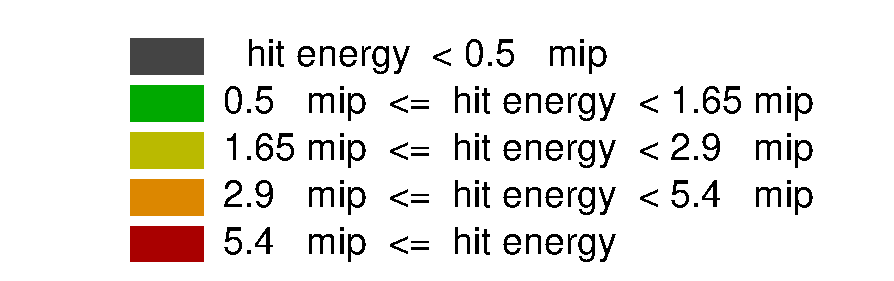
\includegraphics[width=10cm]{EventDisplayProcessor_colorCode}
\caption{C\-E\-D color coding}
\end{DoxyImage}


\begin{DoxyAuthor}{Author}
S. Lu, D\-E\-S\-Y 
\end{DoxyAuthor}
\begin{DoxyVersion}{Version}
1.\-0 
\end{DoxyVersion}
\begin{DoxyDate}{Date}
November 2014
\end{DoxyDate}
Modification \-: E. Brianne, D\-E\-S\-Y Date \-: December 2015 

\subsection{Member Function Documentation}
\index{C\-A\-L\-I\-C\-E\-::\-D\-E\-H\-Event\-Display\-Processor@{C\-A\-L\-I\-C\-E\-::\-D\-E\-H\-Event\-Display\-Processor}!end@{end}}
\index{end@{end}!CALICE::DEHEventDisplayProcessor@{C\-A\-L\-I\-C\-E\-::\-D\-E\-H\-Event\-Display\-Processor}}
\subsubsection[{end}]{\setlength{\rightskip}{0pt plus 5cm}void C\-A\-L\-I\-C\-E\-::\-D\-E\-H\-Event\-Display\-Processor\-::end (
\begin{DoxyParamCaption}
{}
\end{DoxyParamCaption}
)\hspace{0.3cm}{\ttfamily [virtual]}}\label{classCALICE_1_1DEHEventDisplayProcessor_addaf544e8e779e5c423cabdcd7c2bd16}
Called after data processing for clean up. \index{C\-A\-L\-I\-C\-E\-::\-D\-E\-H\-Event\-Display\-Processor@{C\-A\-L\-I\-C\-E\-::\-D\-E\-H\-Event\-Display\-Processor}!init@{init}}
\index{init@{init}!CALICE::DEHEventDisplayProcessor@{C\-A\-L\-I\-C\-E\-::\-D\-E\-H\-Event\-Display\-Processor}}
\subsubsection[{init}]{\setlength{\rightskip}{0pt plus 5cm}void C\-A\-L\-I\-C\-E\-::\-D\-E\-H\-Event\-Display\-Processor\-::init (
\begin{DoxyParamCaption}
{}
\end{DoxyParamCaption}
)\hspace{0.3cm}{\ttfamily [virtual]}}\label{classCALICE_1_1DEHEventDisplayProcessor_aa85bc711c1158c2e6a9cccd54875aec3}
Called at the begin of the job before anything is read. Use to initialize the processor, e.\-g. book histograms. 

References \-\_\-calib\-Container, \-\_\-calib\-Processor\-Name, and \-\_\-map\-T0s.

\index{C\-A\-L\-I\-C\-E\-::\-D\-E\-H\-Event\-Display\-Processor@{C\-A\-L\-I\-C\-E\-::\-D\-E\-H\-Event\-Display\-Processor}!process\-Event@{process\-Event}}
\index{process\-Event@{process\-Event}!CALICE::DEHEventDisplayProcessor@{C\-A\-L\-I\-C\-E\-::\-D\-E\-H\-Event\-Display\-Processor}}
\subsubsection[{process\-Event}]{\setlength{\rightskip}{0pt plus 5cm}void C\-A\-L\-I\-C\-E\-::\-D\-E\-H\-Event\-Display\-Processor\-::process\-Event (
\begin{DoxyParamCaption}
\item[{L\-C\-Event $\ast$}]{evt}
\end{DoxyParamCaption}
)\hspace{0.3cm}{\ttfamily [virtual]}}\label{classCALICE_1_1DEHEventDisplayProcessor_ab10768f77362bd79f8690caf36cd3155}
Called for every event -\/ the working horse. \index{C\-A\-L\-I\-C\-E\-::\-D\-E\-H\-Event\-Display\-Processor@{C\-A\-L\-I\-C\-E\-::\-D\-E\-H\-Event\-Display\-Processor}!process\-Run\-Header@{process\-Run\-Header}}
\index{process\-Run\-Header@{process\-Run\-Header}!CALICE::DEHEventDisplayProcessor@{C\-A\-L\-I\-C\-E\-::\-D\-E\-H\-Event\-Display\-Processor}}
\subsubsection[{process\-Run\-Header}]{\setlength{\rightskip}{0pt plus 5cm}void C\-A\-L\-I\-C\-E\-::\-D\-E\-H\-Event\-Display\-Processor\-::process\-Run\-Header (
\begin{DoxyParamCaption}
\item[{L\-C\-Run\-Header $\ast$}]{run}
\end{DoxyParamCaption}
)\hspace{0.3cm}{\ttfamily [virtual]}}\label{classCALICE_1_1DEHEventDisplayProcessor_a7c60e85bb47247683804ebf8d190bf5a}
Called for every run. 

\subsection{Member Data Documentation}
\index{C\-A\-L\-I\-C\-E\-::\-D\-E\-H\-Event\-Display\-Processor@{C\-A\-L\-I\-C\-E\-::\-D\-E\-H\-Event\-Display\-Processor}!\-\_\-calib\-Container@{\-\_\-calib\-Container}}
\index{\-\_\-calib\-Container@{\-\_\-calib\-Container}!CALICE::DEHEventDisplayProcessor@{C\-A\-L\-I\-C\-E\-::\-D\-E\-H\-Event\-Display\-Processor}}
\subsubsection[{\-\_\-calib\-Container}]{\setlength{\rightskip}{0pt plus 5cm}C\-A\-L\-I\-C\-E\-::\-Mapped\-Container$<$C\-A\-L\-I\-C\-E\-::\-Ahc2\-Calibrations$>$$\ast$ C\-A\-L\-I\-C\-E\-::\-D\-E\-H\-Event\-Display\-Processor\-::\-\_\-calib\-Container\hspace{0.3cm}{\ttfamily [protected]}}\label{classCALICE_1_1DEHEventDisplayProcessor_a6e0a57e1a933e47f300d9c9e0983b0a8}
mapped container of Si\-P\-M calibrations 

Referenced by init().

\index{C\-A\-L\-I\-C\-E\-::\-D\-E\-H\-Event\-Display\-Processor@{C\-A\-L\-I\-C\-E\-::\-D\-E\-H\-Event\-Display\-Processor}!\-\_\-calib\-Processor\-Name@{\-\_\-calib\-Processor\-Name}}
\index{\-\_\-calib\-Processor\-Name@{\-\_\-calib\-Processor\-Name}!CALICE::DEHEventDisplayProcessor@{C\-A\-L\-I\-C\-E\-::\-D\-E\-H\-Event\-Display\-Processor}}
\subsubsection[{\-\_\-calib\-Processor\-Name}]{\setlength{\rightskip}{0pt plus 5cm}std\-::string C\-A\-L\-I\-C\-E\-::\-D\-E\-H\-Event\-Display\-Processor\-::\-\_\-calib\-Processor\-Name\hspace{0.3cm}{\ttfamily [protected]}}\label{classCALICE_1_1DEHEventDisplayProcessor_a11dd1165470ce5fd88021cb068ce75e3}
Calibration Processor Name 

Referenced by init().

\index{C\-A\-L\-I\-C\-E\-::\-D\-E\-H\-Event\-Display\-Processor@{C\-A\-L\-I\-C\-E\-::\-D\-E\-H\-Event\-Display\-Processor}!\-\_\-map\-T0s@{\-\_\-map\-T0s}}
\index{\-\_\-map\-T0s@{\-\_\-map\-T0s}!CALICE::DEHEventDisplayProcessor@{C\-A\-L\-I\-C\-E\-::\-D\-E\-H\-Event\-Display\-Processor}}
\subsubsection[{\-\_\-map\-T0s}]{\setlength{\rightskip}{0pt plus 5cm}std\-::map$<$int, std\-::vector$<$ std\-::pair$<$int, int$>$ $>$ $>$ C\-A\-L\-I\-C\-E\-::\-D\-E\-H\-Event\-Display\-Processor\-::\-\_\-map\-T0s\hspace{0.3cm}{\ttfamily [protected]}}\label{classCALICE_1_1DEHEventDisplayProcessor_a76f178c1dd86aea8af140c2f66d7620d}
map for T0s 

Referenced by init().

\index{C\-A\-L\-I\-C\-E\-::\-D\-E\-H\-Event\-Display\-Processor@{C\-A\-L\-I\-C\-E\-::\-D\-E\-H\-Event\-Display\-Processor}!\-\_\-\-T0\-Vector@{\-\_\-\-T0\-Vector}}
\index{\-\_\-\-T0\-Vector@{\-\_\-\-T0\-Vector}!CALICE::DEHEventDisplayProcessor@{C\-A\-L\-I\-C\-E\-::\-D\-E\-H\-Event\-Display\-Processor}}
\subsubsection[{\-\_\-\-T0\-Vector}]{\setlength{\rightskip}{0pt plus 5cm}String\-Vec C\-A\-L\-I\-C\-E\-::\-D\-E\-H\-Event\-Display\-Processor\-::\-\_\-\-T0\-Vector\hspace{0.3cm}{\ttfamily [protected]}}\label{classCALICE_1_1DEHEventDisplayProcessor_a2cd8fdfd7bdb4292a7f8e049686fa4a2}
Vector containing T0s 

The documentation for this class was generated from the following files\-:\begin{DoxyCompactItemize}
\item 
/nfs/dust/ilc/user/marquezh/\-Calice\-Soft\-\_\-w\-\_\-\-I\-L\-C\-Soft\-\_\-v02-\/03-\/02/calice\-\_\-analysis/addon\-Procs/include/D\-E\-H\-Event\-Display\-Processor.\-hh\item 
/nfs/dust/ilc/user/marquezh/\-Calice\-Soft\-\_\-w\-\_\-\-I\-L\-C\-Soft\-\_\-v02-\/03-\/02/calice\-\_\-analysis/addon\-Procs/src/D\-E\-H\-Event\-Display\-Processor.\-cc\end{DoxyCompactItemize}

\section{C\-A\-L\-I\-C\-E\-:\-:Emc\-Track\-Bit\-Generator Class Reference}
\label{classCALICE_1_1EmcTrackBitGenerator}\index{C\-A\-L\-I\-C\-E\-::\-Emc\-Track\-Bit\-Generator@{C\-A\-L\-I\-C\-E\-::\-Emc\-Track\-Bit\-Generator}}


{\ttfamily \#include $<$Emc\-Track\-Bit\-Generator.\-hh$>$}

Inheritance diagram for C\-A\-L\-I\-C\-E\-:\-:Emc\-Track\-Bit\-Generator\-:\begin{figure}[H]
\begin{center}
\leavevmode
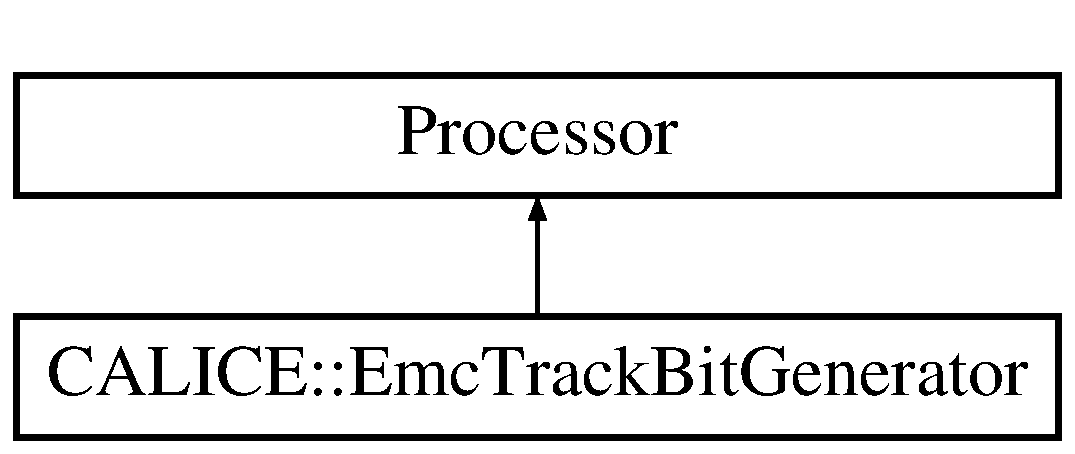
\includegraphics[height=2.000000cm]{classCALICE_1_1EmcTrackBitGenerator}
\end{center}
\end{figure}
\subsection*{Public Member Functions}
\begin{DoxyCompactItemize}
\item 
Processor $\ast$ {\bfseries new\-Processor} ()\label{classCALICE_1_1EmcTrackBitGenerator_a6d7fcff20d6c0d7e8fdfdaa368152375}

\item 
void {\bf init} ()
\item 
void {\bf process\-Run\-Header} (L\-C\-Run\-Header $\ast$run)
\item 
void {\bf process\-Event} (L\-C\-Event $\ast$evt)
\item 
void {\bfseries end} ()\label{classCALICE_1_1EmcTrackBitGenerator_a2724be021e2cc9988cb185c2188a1b35}

\end{DoxyCompactItemize}
\subsection*{Protected Attributes}
\begin{DoxyCompactItemize}
\item 
std\-::string {\bfseries \-\_\-emc\-Hit\-Col\-Name}\label{classCALICE_1_1EmcTrackBitGenerator_a30848a2a5457bd4449356234ae98e5f8}

\item 
std\-::string {\bfseries \-\_\-output\-Par\-Name\-\_\-track\-Bit}\label{classCALICE_1_1EmcTrackBitGenerator_a747d85e775c65db73457bd3b9e216937}

\item 
int {\bfseries \-\_\-max\-Hits}\label{classCALICE_1_1EmcTrackBitGenerator_af1a23b3b8aa6e1b996f469701b016032}

\item 
float {\bfseries \-\_\-max\-E\-Sum}\label{classCALICE_1_1EmcTrackBitGenerator_ae8386f0bac5b67e482ebb0f77c3005e5}

\end{DoxyCompactItemize}


\subsection{Detailed Description}
Processor which generates a trigger bit based on E\-C\-A\-L information. The trigger bit can be used by the \doxyref{Event\-Selector}{p.}{classCALICE_1_1EventSelector}, e.\-g, to select mip-\/like tracks in the E\-C\-A\-L. \begin{DoxyAuthor}{Author}
N. Feege 
\end{DoxyAuthor}
\begin{DoxyDate}{Date}
Sep 2009 
\end{DoxyDate}


\subsection{Member Function Documentation}
\index{C\-A\-L\-I\-C\-E\-::\-Emc\-Track\-Bit\-Generator@{C\-A\-L\-I\-C\-E\-::\-Emc\-Track\-Bit\-Generator}!init@{init}}
\index{init@{init}!CALICE::EmcTrackBitGenerator@{C\-A\-L\-I\-C\-E\-::\-Emc\-Track\-Bit\-Generator}}
\subsubsection[{init}]{\setlength{\rightskip}{0pt plus 5cm}void C\-A\-L\-I\-C\-E\-::\-Emc\-Track\-Bit\-Generator\-::init (
\begin{DoxyParamCaption}
{}
\end{DoxyParamCaption}
)}\label{classCALICE_1_1EmcTrackBitGenerator_ae3d7274d6d4d0e7ca140a1be4288e128}
Called at the begin of the job before anything is read. Use to initialize the processor, e.\-g. book histograms. \index{C\-A\-L\-I\-C\-E\-::\-Emc\-Track\-Bit\-Generator@{C\-A\-L\-I\-C\-E\-::\-Emc\-Track\-Bit\-Generator}!process\-Event@{process\-Event}}
\index{process\-Event@{process\-Event}!CALICE::EmcTrackBitGenerator@{C\-A\-L\-I\-C\-E\-::\-Emc\-Track\-Bit\-Generator}}
\subsubsection[{process\-Event}]{\setlength{\rightskip}{0pt plus 5cm}void C\-A\-L\-I\-C\-E\-::\-Emc\-Track\-Bit\-Generator\-::process\-Event (
\begin{DoxyParamCaption}
\item[{L\-C\-Event $\ast$}]{evt}
\end{DoxyParamCaption}
)}\label{classCALICE_1_1EmcTrackBitGenerator_a77daaa885810c24760881bb5537222eb}
Called for every event -\/ this is where the actual action is taking place. \index{C\-A\-L\-I\-C\-E\-::\-Emc\-Track\-Bit\-Generator@{C\-A\-L\-I\-C\-E\-::\-Emc\-Track\-Bit\-Generator}!process\-Run\-Header@{process\-Run\-Header}}
\index{process\-Run\-Header@{process\-Run\-Header}!CALICE::EmcTrackBitGenerator@{C\-A\-L\-I\-C\-E\-::\-Emc\-Track\-Bit\-Generator}}
\subsubsection[{process\-Run\-Header}]{\setlength{\rightskip}{0pt plus 5cm}void C\-A\-L\-I\-C\-E\-::\-Emc\-Track\-Bit\-Generator\-::process\-Run\-Header (
\begin{DoxyParamCaption}
\item[{L\-C\-Run\-Header $\ast$}]{run}
\end{DoxyParamCaption}
)}\label{classCALICE_1_1EmcTrackBitGenerator_a8d3145cbbe0a7ae871124b1633d43c3e}
Called for every run, e.\-g. overwrite to initialize run dependent histograms. 

The documentation for this class was generated from the following files\-:\begin{DoxyCompactItemize}
\item 
/nfs/dust/ilc/user/marquezh/\-Calice\-Soft\-\_\-w\-\_\-\-I\-L\-C\-Soft\-\_\-v02-\/03-\/02/calice\-\_\-analysis/addon\-Procs/include/Emc\-Track\-Bit\-Generator.\-hh\item 
/nfs/dust/ilc/user/marquezh/\-Calice\-Soft\-\_\-w\-\_\-\-I\-L\-C\-Soft\-\_\-v02-\/03-\/02/calice\-\_\-analysis/addon\-Procs/src/Emc\-Track\-Bit\-Generator.\-cc\end{DoxyCompactItemize}

\section{C\-A\-L\-I\-C\-E\-:\-:Event\-Display\-Processor Class Reference}
\label{classCALICE_1_1EventDisplayProcessor}\index{C\-A\-L\-I\-C\-E\-::\-Event\-Display\-Processor@{C\-A\-L\-I\-C\-E\-::\-Event\-Display\-Processor}}


This is a Marlin processor for displaying events with C\-E\-D.  




{\ttfamily \#include $<$Event\-Display\-Processor.\-hh$>$}

Inheritance diagram for C\-A\-L\-I\-C\-E\-:\-:Event\-Display\-Processor\-:\begin{figure}[H]
\begin{center}
\leavevmode
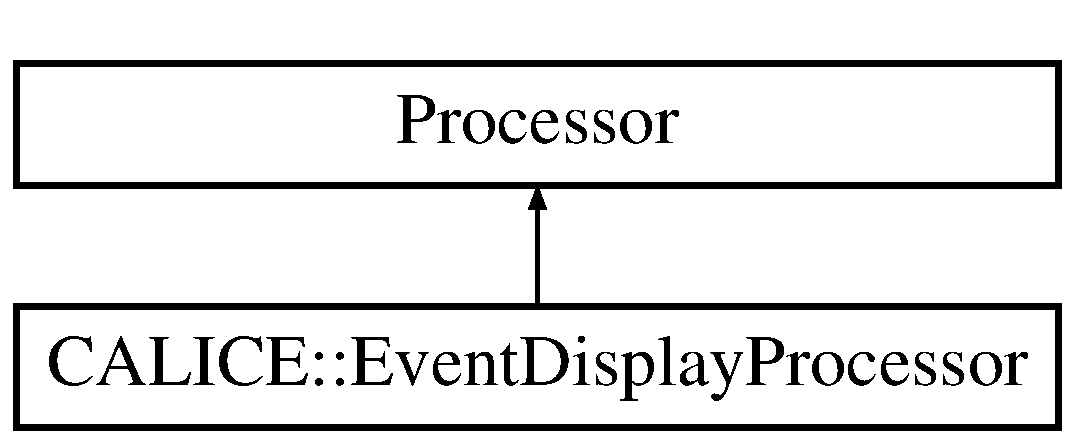
\includegraphics[height=2.000000cm]{classCALICE_1_1EventDisplayProcessor}
\end{center}
\end{figure}
\subsection*{Public Member Functions}
\begin{DoxyCompactItemize}
\item 
virtual Processor $\ast$ {\bfseries new\-Processor} ()\label{classCALICE_1_1EventDisplayProcessor_a34077bee4a0c9c8872846638252f9bac}

\item 
virtual void {\bf init} ()
\item 
virtual void {\bf process\-Run\-Header} (L\-C\-Run\-Header $\ast$run)
\item 
virtual void {\bf process\-Event} (L\-C\-Event $\ast$evt)
\item 
virtual void {\bfseries check} (L\-C\-Event $\ast$evt)\label{classCALICE_1_1EventDisplayProcessor_a60086f666abafbabb0b348a46da34df6}

\item 
virtual void {\bf end} ()
\end{DoxyCompactItemize}
\subsection*{Protected Member Functions}
\begin{DoxyCompactItemize}
\item 
void {\bfseries choose\-Color\-And\-Layer} (const float energy, unsigned int \&color, unsigned int \&layer) const \label{classCALICE_1_1EventDisplayProcessor_a7a616a6bbaaa216e2815a3cfbddb7203}

\item 
void {\bfseries draw\-Cell} (const C\-A\-L\-I\-C\-E\-::\-Cell\-Description $\ast$description, const unsigned int color, const unsigned int layer, const bool solid=true) const \label{classCALICE_1_1EventDisplayProcessor_a8c72e4ed7e45c5126de9d0a6a935a9b6}

\item 
void {\bfseries draw\-Hit} (const Calorimeter\-Hit $\ast$hit, const unsigned int color, const unsigned int layer) const \label{classCALICE_1_1EventDisplayProcessor_ab997ab7811aec0cb61ca9a5296796ea9}

\item 
void {\bfseries draw\-Si\-W\-E\-C\-A\-L} (L\-C\-Event $\ast$evt)\label{classCALICE_1_1EventDisplayProcessor_a282a9f9031e3952e9553e22331911935}

\item 
void {\bfseries draw\-A\-H\-C\-A\-L} (L\-C\-Event $\ast$evt)\label{classCALICE_1_1EventDisplayProcessor_af954c017bda60aa0c29a56801da58237}

\item 
void {\bfseries draw\-A\-H\-C\-A\-L\-Tracks} (L\-C\-Event $\ast$evt)\label{classCALICE_1_1EventDisplayProcessor_ae42429db28c5cef293f9cda49d98832e}

\item 
void {\bfseries draw\-A\-H\-C\-A\-L\-Sim} (L\-C\-Event $\ast$evt)\label{classCALICE_1_1EventDisplayProcessor_a695ddbd7d3de1cfc87141ec2f0f98119}

\item 
void {\bfseries draw\-T\-C\-M\-T} (L\-C\-Event $\ast$evt)\label{classCALICE_1_1EventDisplayProcessor_ac6ac2a1b2dff7057d26b3b7318c594fd}

\item 
void {\bf draw\-Start\-Layer} (L\-C\-Event $\ast$evt)
\item 
void {\bfseries draw\-Start\-Position} (L\-C\-Event $\ast$evt)\label{classCALICE_1_1EventDisplayProcessor_a2a0448c458baa43fb23291e86f7c9e0d}

\item 
void {\bfseries draw\-M\-C\-Particle} (L\-C\-Event $\ast$evt)\label{classCALICE_1_1EventDisplayProcessor_adcd63eabf525ce9235e4f1efffe7e4c3}

\item 
void {\bfseries draw\-Detector\-Si\-W\-E\-C\-A\-L} ()\label{classCALICE_1_1EventDisplayProcessor_aac49af6eceba5d02db9d405a42f229ec}

\item 
void {\bfseries draw\-Detector\-A\-H\-C\-A\-L} ()\label{classCALICE_1_1EventDisplayProcessor_acfdc0d075c062b1da8b297e0168405ca}

\item 
void {\bfseries draw\-Detector\-T\-C\-M\-T} ()\label{classCALICE_1_1EventDisplayProcessor_ad489bc345d421518f05340e2b7268365}

\item 
int {\bfseries get\-Marina\-Shower\-Start\-Hcal\-Layer} (L\-C\-Event $\ast$evt)\label{classCALICE_1_1EventDisplayProcessor_a087a520d52e265e7e46b59b8e226028b}

\item 
void {\bfseries draw\-Primary\-Track\-Hits\-Position} (L\-C\-Event $\ast$evt)\label{classCALICE_1_1EventDisplayProcessor_a938088e50170b4c44ea47a5e0e7d2710}

\item 
void {\bfseries draw\-Shower\-Shapes} (L\-C\-Event $\ast$evt)\label{classCALICE_1_1EventDisplayProcessor_a71e596ddf97ee37c2314b474a35eb15a}

\item 
int {\bf return\-Cluster\-Size} (float ene\-Cluster, float cutoff\-\_\-min, float cutoff\-\_\-max)
\end{DoxyCompactItemize}
\subsection*{Protected Attributes}
\begin{DoxyCompactItemize}
\item 
std\-::string {\bfseries \-\_\-col\-Name\-Emc}\label{classCALICE_1_1EventDisplayProcessor_a1efe06a3acf7c317dcfb1d5822c03e68}

\item 
std\-::string {\bfseries \-\_\-col\-Name\-Ahc}\label{classCALICE_1_1EventDisplayProcessor_a8ff444f1b4b4e64a5ea06e30e4f8accf}

\item 
std\-::string {\bfseries \-\_\-col\-Name\-Ahc\-Sim}\label{classCALICE_1_1EventDisplayProcessor_af630ea20517ca82a2e48f59cce5eaf05}

\item 
std\-::string {\bfseries \-\_\-col\-Name\-Tcm}\label{classCALICE_1_1EventDisplayProcessor_a9a05be2ec278b8ec385b7b41957024aa}

\item 
std\-::string {\bfseries \-\_\-col\-Name\-Tcm\-Sim}\label{classCALICE_1_1EventDisplayProcessor_aa5fe137ac3cba3ee963303fc38444cca}

\item 
std\-::string {\bfseries \-\_\-col\-Name\-M\-C\-Particle}\label{classCALICE_1_1EventDisplayProcessor_a7169df856c690f8a76210cf49be08b95}

\item 
std\-::string {\bfseries \-\_\-par\-Name\-Shower\-Start\-Layer}\label{classCALICE_1_1EventDisplayProcessor_afd62efd0e2ac21fb8d69196b2ad1007c}

\item 
std\-::string {\bfseries \-\_\-par\-Name\-Shower\-Start\-Pos}\label{classCALICE_1_1EventDisplayProcessor_a5c8b338ab8395474cdfe6e1ae97828ac}

\item 
std\-::string {\bfseries \-\_\-mapping\-Processor\-Name}\label{classCALICE_1_1EventDisplayProcessor_a7e2048023fb976e1ad4595143e82c2eb}

\item 
std\-::string {\bfseries \-\_\-cell\-Neighbours\-Processor\-Name}\label{classCALICE_1_1EventDisplayProcessor_a7a6c899ee6fed94746b5bed528908523}

\item 
std\-::string {\bfseries \-\_\-cell\-Description\-Processor\-Name}\label{classCALICE_1_1EventDisplayProcessor_a28820140d1bc43b3f09f9b507f19867a}

\item 
std\-::string {\bfseries \-\_\-f\-Mokka\-Model\-Name}\label{classCALICE_1_1EventDisplayProcessor_aa5b896435eb4c373970396fac01e050c}

\item 
std\-::string {\bfseries \-\_\-shower\-Shape\-Col\-Names}\label{classCALICE_1_1EventDisplayProcessor_a4946742dffb613191debad2305a9d4be}

\item 
std\-::string {\bfseries \-\_\-track\-Col\-Name}\label{classCALICE_1_1EventDisplayProcessor_a41d1d71e48d0ff487039549ed37cfe3e}

\item 
int {\bfseries \-\_\-wait\-For\-Key\-Pressed}\label{classCALICE_1_1EventDisplayProcessor_a32366f61a3fe9a3903ecf839a64a6689}

\item 
int {\bfseries \-\_\-draw}\label{classCALICE_1_1EventDisplayProcessor_a825f3f4c242a9762e79259e885f1adb2}

\item 
int {\bfseries \-\_\-append\-To\-Existing\-C\-E\-D}\label{classCALICE_1_1EventDisplayProcessor_a687eaf39c649eee27c749b448cdaf986}

\item 
int {\bfseries \-\_\-n\-Run}\label{classCALICE_1_1EventDisplayProcessor_ae6c8eb83553b91997dbacec716e0fd4c}

\item 
int {\bfseries \-\_\-n\-Evt}\label{classCALICE_1_1EventDisplayProcessor_ac73308944a57f40de0ffa64b113cbecc}

\item 
const C\-A\-L\-I\-C\-E\-::\-Ahc\-Mapper $\ast$ {\bfseries \-\_\-mapper}\label{classCALICE_1_1EventDisplayProcessor_a2b26430df1aec866f7971e2627da8860}

\item 
unsigned int {\bfseries \-\_\-mapper\-Version}\label{classCALICE_1_1EventDisplayProcessor_a42aea5d31a52a9da2953eeb1e67862b7}

\item 
C\-A\-L\-I\-C\-E\-::\-Mapped\-Container\\*
$<$ C\-A\-L\-I\-C\-E\-::\-Cell\-Description $>$ $\ast$ {\bfseries \-\_\-cell\-Descriptions}\label{classCALICE_1_1EventDisplayProcessor_a94ee4ec40eb5d377d15bc8239e659bb4}

\item 
C\-A\-L\-I\-C\-E\-::\-Mapped\-Container\\*
$<$ C\-A\-L\-I\-C\-E\-::\-Cell\-Neighbours $>$ $\ast$ {\bfseries \-\_\-cell\-Neighbours}\label{classCALICE_1_1EventDisplayProcessor_a12ee00ddafb412fe4f5fffcc9c049e80}

\item 
bool {\bfseries \-\_\-draw\-Hcal\-Histos}\label{classCALICE_1_1EventDisplayProcessor_a6763de26bb6b411cbace86b1df1a6070}

\item 
bool {\bfseries \-\_\-tcmt\-Start\-Vertical}\label{classCALICE_1_1EventDisplayProcessor_a6c010062901aec5839d39d9b54e1719e}

\item 
{\bf Hcal\-Histos\-Drawer} $\ast$ {\bfseries \-\_\-the\-Hcal\-Histos\-Drawer}\label{classCALICE_1_1EventDisplayProcessor_a5b204dde67e52d9a226af122dd6e0573}

\item 
std\-::string {\bfseries \-\_\-shower\-Start\-Col\-Name}\label{classCALICE_1_1EventDisplayProcessor_a91c75bbd29a29d5cdf625a0d5e6b6fcb}

\end{DoxyCompactItemize}


\subsection{Detailed Description}
This is a Marlin processor for displaying events with C\-E\-D. 

If you want to display events with C\-E\-D, you need to start the display ({\ttfamily glced}) before running Marlin.

Mouse commands that can be used within C\-E\-D\-:


\begin{DoxyItemize}
\item {\ttfamily  left + move } -\/$>$ rotate view
\item {\ttfamily  right + move down/up } -\/$>$ zoom view in/out
\item {\ttfamily  center + move } -\/$>$ shift view
\item {\ttfamily  wheel } -\/$>$ shift view along z-\/axis
\end{DoxyItemize}

Keyboard commands that can be used within C\-E\-D\-:


\begin{DoxyItemize}
\item {\ttfamily  b } -\/$>$ toggle background color
\item {\ttfamily  r } -\/$>$ got to default angular view
\item {\ttfamily  s } -\/$>$ got to default side view
\item {\ttfamily  f } -\/$>$ got to default front view
\item {\ttfamily  v } -\/$>$ switch on/off fisheye view
\item {\ttfamily  0 ... 9 } -\/$>$ switch on/off C\-E\-D display layer 0 ... 9
\item {\ttfamily  shift + 0 ... 9 } -\/$>$ switch on/off display layer 10 ... 19
\item {\ttfamily  t } -\/$>$ switch on/off C\-E\-D display layer 20
\item {\ttfamily  y } -\/$>$ switch on/off C\-E\-D display layer 21
\item {\ttfamily  u } -\/$>$ switch on/off C\-E\-D display layer 22
\item {\ttfamily  i } -\/$>$ switch on/off C\-E\-D display layer 23
\end{DoxyItemize}

Assignment of C\-E\-D display layers\-:


\begin{DoxyItemize}
\item 0\-:
\item 1\-: A\-H\-C\-A\-L / E\-C\-A\-L / T\-C\-M\-T hits ( hit energy $<$ 0.\-5 mip )
\item 2\-: A\-H\-C\-A\-L / E\-C\-A\-L / T\-C\-M\-T hits ( 0.\-5 mip $<$= hit energy $<$ 1.\-65 mip )
\item 3\-: A\-H\-C\-A\-L / E\-C\-A\-L / T\-C\-M\-T hits ( 1.\-65 mip $<$= hit energy $<$ 2.\-9 mip )
\item 4\-: A\-H\-C\-A\-L / E\-C\-A\-L / T\-C\-M\-T hits ( 2.\-9 mip $<$= hit energy $<$ 5.\-4 mip )
\item 5\-: A\-H\-C\-A\-L / E\-C\-A\-L / T\-C\-M\-T hits ( hit energy $>$= 5.\-4 mip )
\item 6\-:
\item 7\-:
\item 8\-:
\item 9\-:
\item 10\-:
\item 11\-: M\-C particle track
\item 12\-: shower start layer
\item 13\-: shower start position
\item 14\-:
\item 15\-:
\item 16\-:
\item 17\-:
\item 18\-:
\item 19\-:
\item 20\-: cell frames\-: A\-H\-C\-A\-L hits
\item 21\-: cell frames\-: A\-H\-C\-A\-L tiles 3x3 cm$^\wedge$2
\item 22\-: cell frames\-: A\-H\-C\-A\-L tiles 6x6 cm$^\wedge$2
\item 23\-: cell frames\-: A\-H\-C\-A\-L tiles 12x12 cm$^\wedge$2
\end{DoxyItemize}

C\-E\-D color coding for hit energies\-:

 
\begin{DoxyImage}
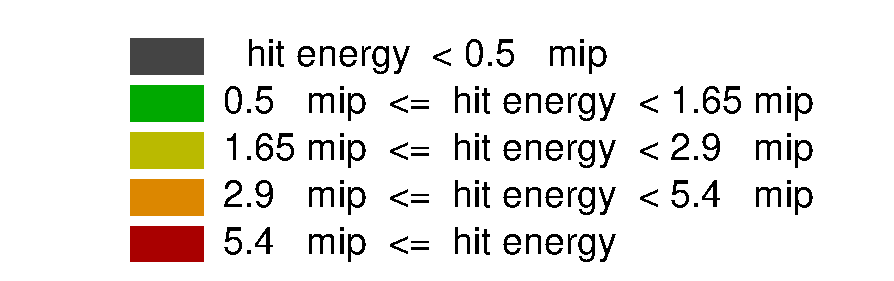
\includegraphics[width=10cm]{EventDisplayProcessor_colorCode}
\caption{C\-E\-D color coding}
\end{DoxyImage}


\begin{DoxyAuthor}{Author}
B. Lutz, D\-E\-S\-Y 

N. Feege, University of Hamburg 
\end{DoxyAuthor}
\begin{DoxyVersion}{Version}
1.\-0 
\end{DoxyVersion}
\begin{DoxyDate}{Date}
April 2010 
\end{DoxyDate}


\subsection{Member Function Documentation}
\index{C\-A\-L\-I\-C\-E\-::\-Event\-Display\-Processor@{C\-A\-L\-I\-C\-E\-::\-Event\-Display\-Processor}!draw\-Start\-Layer@{draw\-Start\-Layer}}
\index{draw\-Start\-Layer@{draw\-Start\-Layer}!CALICE::EventDisplayProcessor@{C\-A\-L\-I\-C\-E\-::\-Event\-Display\-Processor}}
\subsubsection[{draw\-Start\-Layer}]{\setlength{\rightskip}{0pt plus 5cm}void C\-A\-L\-I\-C\-E\-::\-Event\-Display\-Processor\-::draw\-Start\-Layer (
\begin{DoxyParamCaption}
\item[{L\-C\-Event $\ast$}]{evt}
\end{DoxyParamCaption}
)\hspace{0.3cm}{\ttfamily [protected]}}\label{classCALICE_1_1EventDisplayProcessor_aa1a31bdb7c85f8ffa5cce1b1c79d482e}
\begin{DoxyRefDesc}{Todo}
\item[{\bf Todo}]count layers from 1 to 38 or from 0 to 37?? \end{DoxyRefDesc}


Referenced by process\-Event().

\index{C\-A\-L\-I\-C\-E\-::\-Event\-Display\-Processor@{C\-A\-L\-I\-C\-E\-::\-Event\-Display\-Processor}!end@{end}}
\index{end@{end}!CALICE::EventDisplayProcessor@{C\-A\-L\-I\-C\-E\-::\-Event\-Display\-Processor}}
\subsubsection[{end}]{\setlength{\rightskip}{0pt plus 5cm}void C\-A\-L\-I\-C\-E\-::\-Event\-Display\-Processor\-::end (
\begin{DoxyParamCaption}
{}
\end{DoxyParamCaption}
)\hspace{0.3cm}{\ttfamily [virtual]}}\label{classCALICE_1_1EventDisplayProcessor_ade6d63583f10ad947b415e791d3e3700}
Called after data processing for clean up. \index{C\-A\-L\-I\-C\-E\-::\-Event\-Display\-Processor@{C\-A\-L\-I\-C\-E\-::\-Event\-Display\-Processor}!init@{init}}
\index{init@{init}!CALICE::EventDisplayProcessor@{C\-A\-L\-I\-C\-E\-::\-Event\-Display\-Processor}}
\subsubsection[{init}]{\setlength{\rightskip}{0pt plus 5cm}void C\-A\-L\-I\-C\-E\-::\-Event\-Display\-Processor\-::init (
\begin{DoxyParamCaption}
{}
\end{DoxyParamCaption}
)\hspace{0.3cm}{\ttfamily [virtual]}}\label{classCALICE_1_1EventDisplayProcessor_a94bcb2e21a5222c264661c7183e0bfd7}
Called at the begin of the job before anything is read. Use to initialize the processor, e.\-g. book histograms. \index{C\-A\-L\-I\-C\-E\-::\-Event\-Display\-Processor@{C\-A\-L\-I\-C\-E\-::\-Event\-Display\-Processor}!process\-Event@{process\-Event}}
\index{process\-Event@{process\-Event}!CALICE::EventDisplayProcessor@{C\-A\-L\-I\-C\-E\-::\-Event\-Display\-Processor}}
\subsubsection[{process\-Event}]{\setlength{\rightskip}{0pt plus 5cm}void C\-A\-L\-I\-C\-E\-::\-Event\-Display\-Processor\-::process\-Event (
\begin{DoxyParamCaption}
\item[{L\-C\-Event $\ast$}]{evt}
\end{DoxyParamCaption}
)\hspace{0.3cm}{\ttfamily [virtual]}}\label{classCALICE_1_1EventDisplayProcessor_a99a35b6b752fde1e752f6d94a9c0482c}
Called for every event -\/ the working horse. 

References draw\-Start\-Layer().

\index{C\-A\-L\-I\-C\-E\-::\-Event\-Display\-Processor@{C\-A\-L\-I\-C\-E\-::\-Event\-Display\-Processor}!process\-Run\-Header@{process\-Run\-Header}}
\index{process\-Run\-Header@{process\-Run\-Header}!CALICE::EventDisplayProcessor@{C\-A\-L\-I\-C\-E\-::\-Event\-Display\-Processor}}
\subsubsection[{process\-Run\-Header}]{\setlength{\rightskip}{0pt plus 5cm}void C\-A\-L\-I\-C\-E\-::\-Event\-Display\-Processor\-::process\-Run\-Header (
\begin{DoxyParamCaption}
\item[{L\-C\-Run\-Header $\ast$}]{run}
\end{DoxyParamCaption}
)\hspace{0.3cm}{\ttfamily [virtual]}}\label{classCALICE_1_1EventDisplayProcessor_a9a1595afba6f9b8e2369e2e8561983c3}
Called for every run. \index{C\-A\-L\-I\-C\-E\-::\-Event\-Display\-Processor@{C\-A\-L\-I\-C\-E\-::\-Event\-Display\-Processor}!return\-Cluster\-Size@{return\-Cluster\-Size}}
\index{return\-Cluster\-Size@{return\-Cluster\-Size}!CALICE::EventDisplayProcessor@{C\-A\-L\-I\-C\-E\-::\-Event\-Display\-Processor}}
\subsubsection[{return\-Cluster\-Size}]{\setlength{\rightskip}{0pt plus 5cm}int C\-A\-L\-I\-C\-E\-::\-Event\-Display\-Processor\-::return\-Cluster\-Size (
\begin{DoxyParamCaption}
\item[{float}]{ene\-Cluster, }
\item[{float}]{cutoff\-\_\-min, }
\item[{float}]{cutoff\-\_\-max}
\end{DoxyParamCaption}
)\hspace{0.3cm}{\ttfamily [protected]}}\label{classCALICE_1_1EventDisplayProcessor_a5b91c6a831b236cda01569ef41339b8d}
Check the input values for sanity

Check the output 

The documentation for this class was generated from the following files\-:\begin{DoxyCompactItemize}
\item 
/nfs/dust/ilc/user/marquezh/\-Calice\-Soft\-\_\-w\-\_\-\-I\-L\-C\-Soft\-\_\-v02-\/03-\/02/calice\-\_\-analysis/addon\-Procs/include/Event\-Display\-Processor.\-hh\item 
/nfs/dust/ilc/user/marquezh/\-Calice\-Soft\-\_\-w\-\_\-\-I\-L\-C\-Soft\-\_\-v02-\/03-\/02/calice\-\_\-analysis/addon\-Procs/src/Event\-Display\-Processor.\-cc\end{DoxyCompactItemize}

\section{C\-A\-L\-I\-C\-E\-:\-:Event\-Filter Class Reference}
\label{classCALICE_1_1EventFilter}\index{C\-A\-L\-I\-C\-E\-::\-Event\-Filter@{C\-A\-L\-I\-C\-E\-::\-Event\-Filter}}
Inheritance diagram for C\-A\-L\-I\-C\-E\-:\-:Event\-Filter\-:\begin{figure}[H]
\begin{center}
\leavevmode
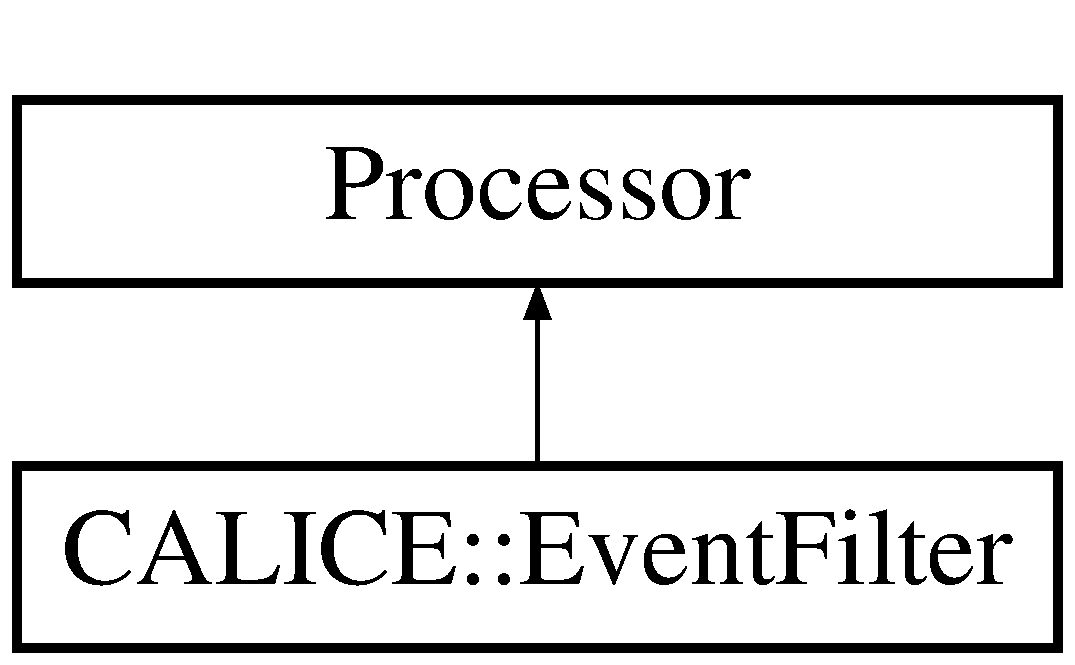
\includegraphics[height=2.000000cm]{classCALICE_1_1EventFilter}
\end{center}
\end{figure}
\subsection*{Public Member Functions}
\begin{DoxyCompactItemize}
\item 
virtual Processor $\ast$ {\bfseries new\-Processor} ()\label{classCALICE_1_1EventFilter_ad6dafa3730aa71f1b034f2a4bdc365c8}

\item 
virtual void {\bfseries init} ()\label{classCALICE_1_1EventFilter_a9803d6de07c86fd14ec07fa133b4e8fb}

\item 
void {\bfseries process\-Event} (L\-C\-Event $\ast$evt)\label{classCALICE_1_1EventFilter_af72b4ac4b19fbd9dbc785b9462f40704}

\item 
void {\bfseries end} ()\label{classCALICE_1_1EventFilter_ad642b8b6aafb0e7a59c6ed38be3d954d}

\end{DoxyCompactItemize}
\subsection*{Protected Attributes}
\begin{DoxyCompactItemize}
\item 
std\-::string {\bfseries \-\_\-dwc\-Col\-Name}\label{classCALICE_1_1EventFilter_a125afd6f12ac67cf85e8e934c0f3e62d}

\item 
std\-::string {\bfseries \-\_\-lay\-Var\-Col\-Name}\label{classCALICE_1_1EventFilter_a2654d519a99b4207fb6424c20acec14b}

\item 
std\-::string {\bfseries \-\_\-evt\-Var\-Col\-Name}\label{classCALICE_1_1EventFilter_a22fdcdb3082038cd84e92d0180caa219}

\item 
std\-::string {\bfseries \-\_\-hit\-In\-Col\-Name}\label{classCALICE_1_1EventFilter_a2dd9d43340604af34fc3d2553d2b02c4}

\item 
bool {\bfseries \-\_\-require\-Track}\label{classCALICE_1_1EventFilter_ab329b6100f8862bb050c56b389f65c45}

\item 
bool {\bfseries \-\_\-require\-Single\-Track}\label{classCALICE_1_1EventFilter_a4d4aba71b20ca1b2862db0d75d51821d}

\item 
bool {\bfseries \-\_\-require\-Track\-Hit\-Match\-Layer1}\label{classCALICE_1_1EventFilter_a93b8d4780b17e2d2fc070db71e6b6c8c}

\item 
bool {\bfseries \-\_\-require\-Track\-Hit\-Match\-Layer1or2or3}\label{classCALICE_1_1EventFilter_a9d7277aae041df1fc56f8603c5f2fe9e}

\item 
float {\bfseries \-\_\-maxr}\label{classCALICE_1_1EventFilter_a6c208e4a94adf820fcb8da72c384620a}

\item 
int {\bfseries \-\_\-kfirst\-A\-H\-C\-A\-Llayer}\label{classCALICE_1_1EventFilter_ad27c08374fb865409fb2316e12111992}

\item 
bool {\bfseries \-\_\-hitin\-Layer1}\label{classCALICE_1_1EventFilter_a76a1915d609bb8217d07c80ba988b489}

\item 
bool {\bfseries \-\_\-hitin\-Layer2}\label{classCALICE_1_1EventFilter_a262a3a3a6c20df71fad5104eee4ff237}

\item 
bool {\bfseries \-\_\-hitin\-Layer3}\label{classCALICE_1_1EventFilter_a08bf1f9e0f910d28430f37eb74d5274b}

\item 
bool {\bfseries \-\_\-hitin\-Layer1or2or3}\label{classCALICE_1_1EventFilter_a00eb1957c50ee409c88bf6c0783288d4}

\item 
bool {\bfseries \-\_\-filternoshowering}\label{classCALICE_1_1EventFilter_a12d4e0cce8751ec9c6646d74f9c348c0}

\item 
bool {\bfseries \-\_\-apply\-\_\-showerstartupperlimit}\label{classCALICE_1_1EventFilter_a4048050dad7af244743d367aeb2852cd}

\item 
int {\bfseries \-\_\-showerstart\-\_\-upper\-\_\-limit}\label{classCALICE_1_1EventFilter_a978ba19843e906ebd72fbb1408217094}

\item 
bool {\bfseries \-\_\-apply\-\_\-max\-E}\label{classCALICE_1_1EventFilter_a773d99afe89bc3a391f756dd8150acae}

\item 
float {\bfseries \-\_\-max\-E}\label{classCALICE_1_1EventFilter_a907becf7b54c9484c0341f4c0bfec67c}

\item 
bool {\bfseries \-\_\-apply\-\_\-gap\-\_\-rej}\label{classCALICE_1_1EventFilter_a871f6d00a29b90b8569950de529c4e23}

\item 
float {\bfseries \-\_\-gap\-\_\-width}\label{classCALICE_1_1EventFilter_a85b5dce7dc62cec7b77b16c2d114121c}

\item 
float {\bfseries \-\_\-xoffset}\label{classCALICE_1_1EventFilter_a57519587aefeb6c7cc3e3f9914d16c1c}

\item 
float {\bfseries \-\_\-yoffset}\label{classCALICE_1_1EventFilter_a8aeb445a342ec9212f341049881561e6}

\end{DoxyCompactItemize}


The documentation for this class was generated from the following files\-:\begin{DoxyCompactItemize}
\item 
/nfs/dust/ilc/user/marquezh/\-Calice\-Soft\-\_\-w\-\_\-\-I\-L\-C\-Soft\-\_\-v02-\/03-\/02/calice\-\_\-analysis/addon\-Procs/include/Event\-Filter.\-hh\item 
/nfs/dust/ilc/user/marquezh/\-Calice\-Soft\-\_\-w\-\_\-\-I\-L\-C\-Soft\-\_\-v02-\/03-\/02/calice\-\_\-analysis/addon\-Procs/src/Event\-Filter.\-cc\end{DoxyCompactItemize}

\section{C\-A\-L\-I\-C\-E\-:\-:Event\-List\-Processor Class Reference}
\label{classCALICE_1_1EventListProcessor}\index{C\-A\-L\-I\-C\-E\-::\-Event\-List\-Processor@{C\-A\-L\-I\-C\-E\-::\-Event\-List\-Processor}}
Inheritance diagram for C\-A\-L\-I\-C\-E\-:\-:Event\-List\-Processor\-:\begin{figure}[H]
\begin{center}
\leavevmode
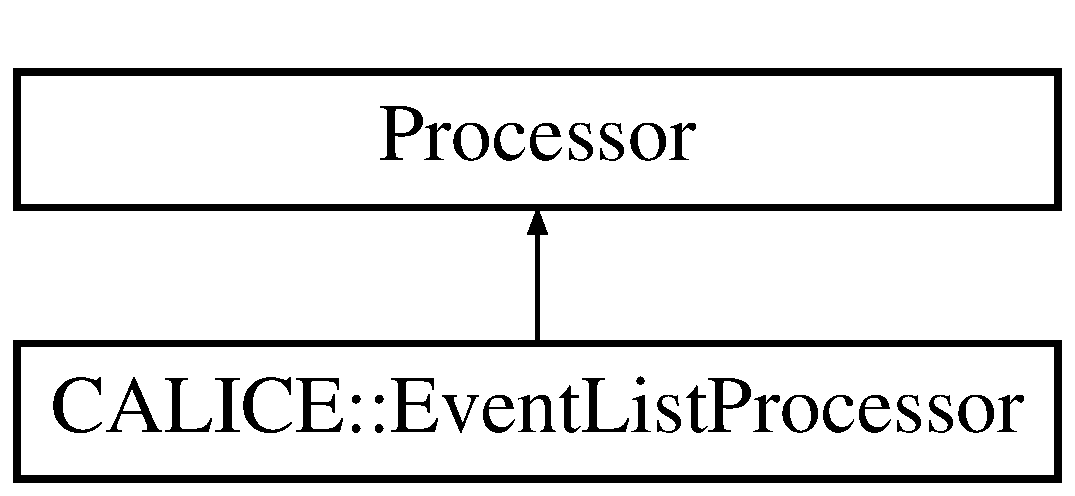
\includegraphics[height=2.000000cm]{classCALICE_1_1EventListProcessor}
\end{center}
\end{figure}
\subsection*{Classes}
\begin{DoxyCompactItemize}
\item 
struct {\bf Run\-Event}
\end{DoxyCompactItemize}
\subsection*{Public Member Functions}
\begin{DoxyCompactItemize}
\item 
virtual Processor $\ast$ {\bfseries new\-Processor} ()\label{classCALICE_1_1EventListProcessor_a23be03857951c989b63af81d518564e9}

\item 
virtual void {\bfseries init} ()\label{classCALICE_1_1EventListProcessor_aa963b574bae85f4290f8ee22572ada31}

\item 
virtual void {\bfseries process\-Event} (E\-V\-E\-N\-T\-::\-L\-C\-Event $\ast$)\label{classCALICE_1_1EventListProcessor_a18ed652b62d32832397bc5c7a8fd698b}

\end{DoxyCompactItemize}
\subsection*{Protected Types}
\begin{DoxyCompactItemize}
\item 
typedef std\-::vector$<$ {\bf Run\-Event} $>$ {\bfseries Event\-List}\label{classCALICE_1_1EventListProcessor_a6900af21cf795245d9e295277dba761c}

\item 
typedef Event\-List\-::const\-\_\-iterator {\bfseries Event\-List\-Iter}\label{classCALICE_1_1EventListProcessor_a1016f6cc849ec0898035ca82bae77876}

\end{DoxyCompactItemize}
\subsection*{Protected Member Functions}
\begin{DoxyCompactItemize}
\item 
void {\bfseries seek\-Next\-Run} ()\label{classCALICE_1_1EventListProcessor_ae343cf6f6cefa042a8cc0dedb6e10270}

\item 
void {\bfseries seek\-Event\-After} (int)\label{classCALICE_1_1EventListProcessor_a76b0e99806b8c34790e5d8a1da36b279}

\end{DoxyCompactItemize}
\subsection*{Protected Attributes}
\begin{DoxyCompactItemize}
\item 
std\-::string {\bfseries \-\_\-event\-List\-Filename}\label{classCALICE_1_1EventListProcessor_ab8779b7ff00ca329ec3195ede9558ce3}

\item 
std\-::fstream {\bfseries \-\_\-event\-List\-F\-Stream}\label{classCALICE_1_1EventListProcessor_a9e5afcb38c4a88ad22214ba552e97671}

\item 
bool {\bfseries \-\_\-skip\-All}\label{classCALICE_1_1EventListProcessor_a8f2c9676aeded88f48b3a203c19069a8}

\item 
Event\-List {\bfseries \-\_\-event\-List}\label{classCALICE_1_1EventListProcessor_a2b73e686f4ea3b6575dd77448017d89c}

\item 
Event\-List\-Iter {\bfseries \-\_\-next\-Event}\label{classCALICE_1_1EventListProcessor_a42a9da251da35720e119cc0c7d48c043}

\end{DoxyCompactItemize}


The documentation for this class was generated from the following files\-:\begin{DoxyCompactItemize}
\item 
/nfs/dust/ilc/user/marquezh/\-Calice\-Soft\-\_\-w\-\_\-\-I\-L\-C\-Soft\-\_\-v02-\/03-\/02/calice\-\_\-analysis/addon\-Procs/include/Event\-List\-Processor.\-hh\item 
/nfs/dust/ilc/user/marquezh/\-Calice\-Soft\-\_\-w\-\_\-\-I\-L\-C\-Soft\-\_\-v02-\/03-\/02/calice\-\_\-analysis/addon\-Procs/src/Event\-List\-Processor.\-cc\end{DoxyCompactItemize}

\section{C\-A\-L\-I\-C\-E\-:\-:Event\-Numbering\-Processor Class Reference}
\label{classCALICE_1_1EventNumberingProcessor}\index{C\-A\-L\-I\-C\-E\-::\-Event\-Numbering\-Processor@{C\-A\-L\-I\-C\-E\-::\-Event\-Numbering\-Processor}}
Inheritance diagram for C\-A\-L\-I\-C\-E\-:\-:Event\-Numbering\-Processor\-:\begin{figure}[H]
\begin{center}
\leavevmode
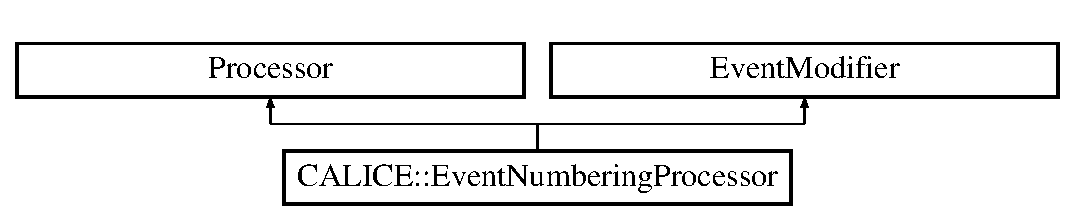
\includegraphics[height=2.000000cm]{classCALICE_1_1EventNumberingProcessor}
\end{center}
\end{figure}
\subsection*{Public Member Functions}
\begin{DoxyCompactItemize}
\item 
virtual Processor $\ast$ {\bfseries new\-Processor} ()\label{classCALICE_1_1EventNumberingProcessor_a38e5409171785827ce12503947b08f5e}

\item 
virtual const std\-::string \& {\bfseries name} () const \label{classCALICE_1_1EventNumberingProcessor_ad8c2e530a6e0a5540d642116145cb512}

\item 
virtual void {\bfseries modify\-Event} (L\-C\-Event $\ast$evt)\label{classCALICE_1_1EventNumberingProcessor_afae9d8d083141ce67dff5c46136b96e7}

\item 
virtual void {\bfseries init} ()\label{classCALICE_1_1EventNumberingProcessor_a9de7055f49f0fa959bad3f5eaf0af4e2}

\item 
virtual void {\bfseries process\-Run\-Header} (L\-C\-Run\-Header $\ast$run)\label{classCALICE_1_1EventNumberingProcessor_ad440173c4d8ba8569360e822f645ba98}

\item 
virtual void {\bfseries check} (L\-C\-Event $\ast$evt)\label{classCALICE_1_1EventNumberingProcessor_a5f2c6d236e6fb61a823c879db688d4e3}

\item 
virtual void {\bfseries end} ()\label{classCALICE_1_1EventNumberingProcessor_a3a59bda8669f25327cf20f4ceda8cc54}

\end{DoxyCompactItemize}


The documentation for this class was generated from the following files\-:\begin{DoxyCompactItemize}
\item 
/nfs/dust/ilc/user/marquezh/\-Calice\-Soft\-\_\-w\-\_\-\-I\-L\-C\-Soft\-\_\-v02-\/03-\/02/calice\-\_\-analysis/addon\-Procs/include/Event\-Numbering\-Processor.\-hh\item 
/nfs/dust/ilc/user/marquezh/\-Calice\-Soft\-\_\-w\-\_\-\-I\-L\-C\-Soft\-\_\-v02-\/03-\/02/calice\-\_\-analysis/addon\-Procs/src/Event\-Numbering\-Processor.\-cc\end{DoxyCompactItemize}

\section{C\-A\-L\-I\-C\-E\-:\-:Event\-Selector Class Reference}
\label{classCALICE_1_1EventSelector}\index{C\-A\-L\-I\-C\-E\-::\-Event\-Selector@{C\-A\-L\-I\-C\-E\-::\-Event\-Selector}}
Inheritance diagram for C\-A\-L\-I\-C\-E\-:\-:Event\-Selector\-:\begin{figure}[H]
\begin{center}
\leavevmode
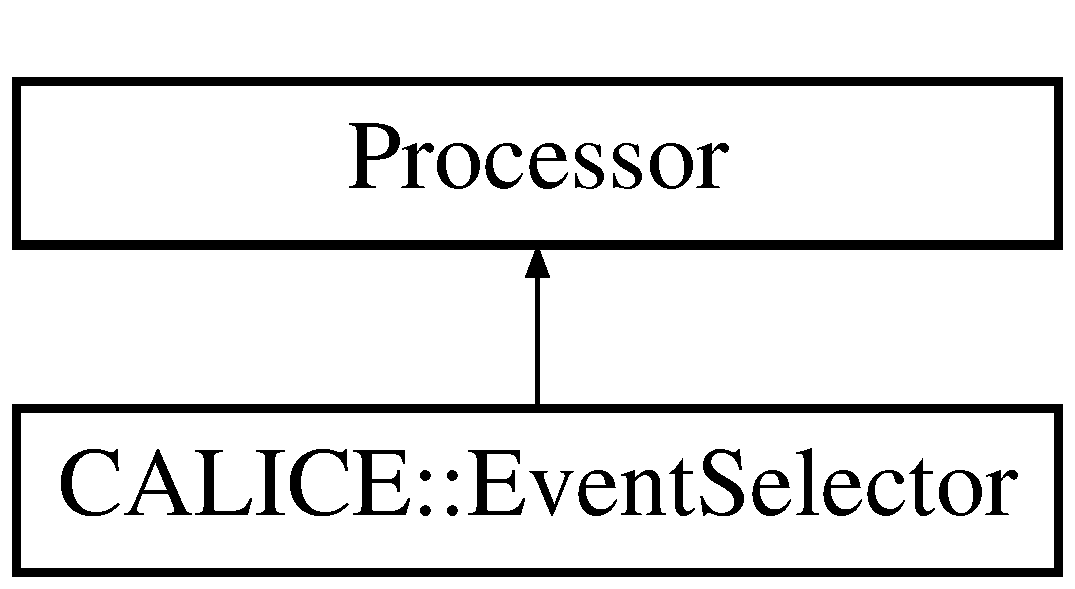
\includegraphics[height=2.000000cm]{classCALICE_1_1EventSelector}
\end{center}
\end{figure}
\subsection*{Public Member Functions}
\begin{DoxyCompactItemize}
\item 
virtual Processor $\ast$ {\bfseries new\-Processor} ()\label{classCALICE_1_1EventSelector_a36b81e0575a2e14335f47a5084f4f3b2}

\item 
virtual void {\bfseries init} ()\label{classCALICE_1_1EventSelector_a6e9b4eb3db9cc056bbdc2c3aaa265273}

\item 
void {\bfseries process\-Event} (L\-C\-Event $\ast$evt)\label{classCALICE_1_1EventSelector_aae415b2d0ced1750d9c93c7318b8953a}

\item 
void {\bfseries end} ()\label{classCALICE_1_1EventSelector_a41de050eb673f31568813d9e9854ed4e}

\end{DoxyCompactItemize}
\subsection*{Protected Attributes}
\begin{DoxyCompactItemize}
\item 
std\-::string {\bfseries \-\_\-par\-Name\-Trigger\-Conf}\label{classCALICE_1_1EventSelector_a55a6011de7b0d8172b22d43e4a56debc}

\item 
std\-::string {\bfseries \-\_\-par\-Name\-Trigger\-Event}\label{classCALICE_1_1EventSelector_a4b4baca2f3f77e95cd862d838685943a}

\item 
std\-::string {\bfseries \-\_\-par\-Name\-Multi\-Bit}\label{classCALICE_1_1EventSelector_a0fa26085b0edc026bed4327de8484f5c}

\item 
std\-::string {\bfseries \-\_\-par\-Name\-Emc\-Track\-Bit}\label{classCALICE_1_1EventSelector_abd154eefb301761d2f81e0140c345f8c}

\item 
std\-::string {\bfseries \-\_\-par\-Name\-Aux\-Bit\-\_\-1}\label{classCALICE_1_1EventSelector_ac18402539a3ccc1bbca3f8f6d6af8352}

\item 
std\-::string {\bfseries \-\_\-par\-Name\-Aux\-Bit\-\_\-2}\label{classCALICE_1_1EventSelector_ab3c66ddc0fcae41c5852d3fe37e7da5a}

\item 
std\-::string {\bfseries \-\_\-par\-Name\-Aux\-Bit\-\_\-3}\label{classCALICE_1_1EventSelector_aa0ff952248fde6503c116cfdb50aca69}

\item 
std\-::string {\bfseries \-\_\-par\-Name\-Aux\-Bit\-\_\-4}\label{classCALICE_1_1EventSelector_ac8b4bcd0d83832ce8a730278c71841cb}

\item 
std\-::string {\bfseries \-\_\-par\-Name\-Aux\-Bit\-\_\-5}\label{classCALICE_1_1EventSelector_a33d71bde813c37e031c471a355553553}

\item 
int {\bfseries \-\_\-skip\-Event\-Number}\label{classCALICE_1_1EventSelector_aca6cfa2d32b5c09f69596c7ba552f23b}

\item 
bool {\bfseries \-\_\-do\-Skip\-Event}\label{classCALICE_1_1EventSelector_aabe06d7a66486b7ffbba539699929e87}

\item 
String\-Vec {\bfseries \-\_\-with\-Triggers}\label{classCALICE_1_1EventSelector_ab6647a10b50b6daed53294286c912c2f}

\item 
String\-Vec {\bfseries \-\_\-without\-Triggers}\label{classCALICE_1_1EventSelector_a5197c32c6f221c58c770bdbce085ecfb}

\end{DoxyCompactItemize}


The documentation for this class was generated from the following files\-:\begin{DoxyCompactItemize}
\item 
/nfs/dust/ilc/user/marquezh/\-Calice\-Soft\-\_\-w\-\_\-\-I\-L\-C\-Soft\-\_\-v02-\/03-\/02/calice\-\_\-analysis/addon\-Procs/include/Event\-Selector.\-hh\item 
/nfs/dust/ilc/user/marquezh/\-Calice\-Soft\-\_\-w\-\_\-\-I\-L\-C\-Soft\-\_\-v02-\/03-\/02/calice\-\_\-analysis/addon\-Procs/src/Event\-Selector.\-cc\end{DoxyCompactItemize}

\section{Hcal\-Track2\-Root\-Tree\-:\-:Event\-Tracks Struct Reference}
\label{structHcalTrack2RootTree_1_1EventTracks}\index{Hcal\-Track2\-Root\-Tree\-::\-Event\-Tracks@{Hcal\-Track2\-Root\-Tree\-::\-Event\-Tracks}}
\subsection*{Public Attributes}
\begin{DoxyCompactItemize}
\item 
Int\-\_\-t {\bfseries idx}\label{structHcalTrack2RootTree_1_1EventTracks_ad0cfcaf5d1c739ea38d6d05379e70d46}

\item 
Int\-\_\-t {\bfseries Run\-No}\label{structHcalTrack2RootTree_1_1EventTracks_a72f2818d16ddc07c2788693d7146feee}

\item 
Int\-\_\-t {\bfseries Evt\-No}\label{structHcalTrack2RootTree_1_1EventTracks_a0c8df9e977ab81885c242e19a0f41c30}

\item 
Int\-\_\-t {\bfseries N\-Tracks}\label{structHcalTrack2RootTree_1_1EventTracks_ab58502846543030fab294e43a8019273}

\item 
Double\-\_\-t {\bfseries Emc\-Energy}\label{structHcalTrack2RootTree_1_1EventTracks_afed7fbe98b7c1f1a2aaaf469ca144237}

\item 
Double\-\_\-t {\bfseries Ahc\-Energy}\label{structHcalTrack2RootTree_1_1EventTracks_a02444b4090c362423d120c984e77f257}

\item 
Double\-\_\-t {\bfseries Tcmt\-Energy}\label{structHcalTrack2RootTree_1_1EventTracks_a34ec7af2977a4fcd1d4e035020516de7}

\item 
std\-::vector$<$ Int\-\_\-t $>$ {\bfseries t\-\_\-\-N\-Hits}\label{structHcalTrack2RootTree_1_1EventTracks_aa6be816c60658808b3cd83c15b5d405d}

\item 
std\-::vector$<$ Int\-\_\-t $>$ {\bfseries t\-\_\-\-N\-Length}\label{structHcalTrack2RootTree_1_1EventTracks_a783113a6c4ada573e45cc0e7ece5a16e}

\item 
std\-::vector$<$ Int\-\_\-t $>$ {\bfseries t\-\_\-\-Start\-Layer}\label{structHcalTrack2RootTree_1_1EventTracks_a47ecd9b7591f4e5485fda74c1c2672bd}

\item 
std\-::vector$<$ Int\-\_\-t $>$ {\bfseries t\-\_\-\-Stop\-Layer}\label{structHcalTrack2RootTree_1_1EventTracks_ae32fb76d840130f1fbe43953298c06eb}

\item 
std\-::vector$<$ Double\-\_\-t $>$ {\bfseries t\-\_\-\-Cos\-Phi}\label{structHcalTrack2RootTree_1_1EventTracks_a3a1a5db72d1428deed0eca93681c6d37}

\item 
std\-::vector$<$ Int\-\_\-t $>$ {\bfseries t\-\_\-track\-Hit\-Index}\label{structHcalTrack2RootTree_1_1EventTracks_a3ee6bda84967e39d8420784d7c81e022}

\item 
std\-::vector$<$ Double\-\_\-t $>$ {\bfseries t\-\_\-h\-\_\-\-Energy}\label{structHcalTrack2RootTree_1_1EventTracks_a87049feb6b6b6da4118db597631025e5}

\item 
std\-::vector$<$ Int\-\_\-t $>$ {\bfseries t\-\_\-h\-\_\-\-I}\label{structHcalTrack2RootTree_1_1EventTracks_a10f85c6012ecdfa9af4c263e39ed9053}

\item 
std\-::vector$<$ Int\-\_\-t $>$ {\bfseries t\-\_\-h\-\_\-\-J}\label{structHcalTrack2RootTree_1_1EventTracks_a167e2ce014c7f8d4b0607abf2e79d948}

\item 
std\-::vector$<$ Int\-\_\-t $>$ {\bfseries t\-\_\-h\-\_\-\-K}\label{structHcalTrack2RootTree_1_1EventTracks_af635a6fba097932e5915b97e4afff06e}

\end{DoxyCompactItemize}


The documentation for this struct was generated from the following file\-:\begin{DoxyCompactItemize}
\item 
/nfs/dust/ilc/user/marquezh/\-Calice\-Soft\-\_\-w\-\_\-\-I\-L\-C\-Soft\-\_\-v02-\/03-\/02/calice\-\_\-analysis/addon\-Procs/include/Hcal\-Track2\-Root\-Tree.\-hh\end{DoxyCompactItemize}

\section{Extract\-Beam\-Energy\-Processor Class Reference}
\label{classExtractBeamEnergyProcessor}\index{Extract\-Beam\-Energy\-Processor@{Extract\-Beam\-Energy\-Processor}}
Inheritance diagram for Extract\-Beam\-Energy\-Processor\-:\begin{figure}[H]
\begin{center}
\leavevmode
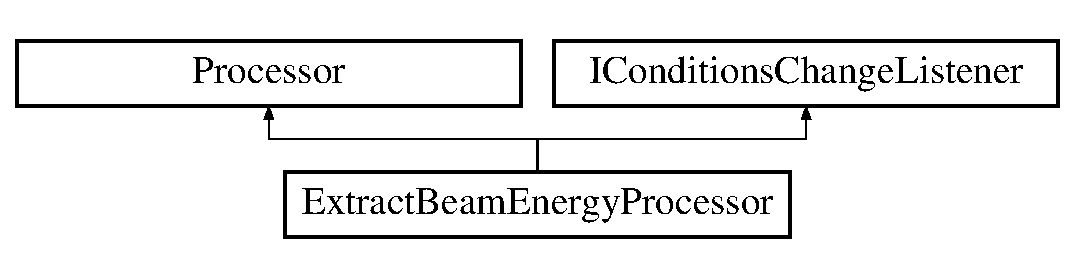
\includegraphics[height=2.000000cm]{classExtractBeamEnergyProcessor}
\end{center}
\end{figure}
\subsection*{Public Member Functions}
\begin{DoxyCompactItemize}
\item 
{\bf Extract\-Beam\-Energy\-Processor} $\ast$ {\bfseries new\-Processor} ()\label{classExtractBeamEnergyProcessor_ac6abcb9dbb0f7237b8b8779496acd9e2}

\item 
virtual void {\bfseries init} ()\label{classExtractBeamEnergyProcessor_a0eac13d2b34280c8ae1a72c6da28f0eb}

\item 
virtual void {\bfseries process\-Event} (lcio\-::\-L\-C\-Event $\ast$)\label{classExtractBeamEnergyProcessor_a3a3d92d23bfba19e22c7e9f9cc4a94e8}

\item 
virtual void {\bfseries end} ()\label{classExtractBeamEnergyProcessor_a3e42907216567e34b02436c664fad568}

\end{DoxyCompactItemize}


The documentation for this class was generated from the following files\-:\begin{DoxyCompactItemize}
\item 
/nfs/dust/ilc/user/marquezh/\-Calice\-Soft\-\_\-w\-\_\-\-I\-L\-C\-Soft\-\_\-v02-\/03-\/02/calice\-\_\-analysis/addon\-Procs/include/Extract\-Beam\-Energy\-Processor.\-hh\item 
/nfs/dust/ilc/user/marquezh/\-Calice\-Soft\-\_\-w\-\_\-\-I\-L\-C\-Soft\-\_\-v02-\/03-\/02/calice\-\_\-analysis/addon\-Procs/src/Extract\-Beam\-Energy\-Processor.\-cc\end{DoxyCompactItemize}

\section{Find\-Start\-And\-Primary\-Track Class Reference}
\label{classFindStartAndPrimaryTrack}\index{Find\-Start\-And\-Primary\-Track@{Find\-Start\-And\-Primary\-Track}}
\subsection*{Public Member Functions}
\begin{DoxyCompactItemize}
\item 
{\bf Find\-Start\-And\-Primary\-Track} (float, int, float)
\begin{DoxyCompactList}\small\item\em First interaction layer and primary track finder. \end{DoxyCompactList}\item 
{\bf $\sim$\-Find\-Start\-And\-Primary\-Track} ()
\item 
float {\bf dist\-X\-Y} (float, float, float, float)
\item 
int {\bf get\-Start\-Layer\-Mip} (std\-::vector$<$ {\bf C\-Layer} $>$, int, int, float, int)
\item 
int {\bf get\-Start\-Layer\-Nei} (std\-::vector$<$ {\bf C\-Layer} $>$, int)
\item 
int {\bf Find\-Track} (int, float, float, bool, int, int, int, int, {\bf C\-Layer} $\ast$, bool)
\item 
bool {\bf get\-Number\-Of\-Neighbors} ({\bf C\-Hit}, std\-::vector$<$ {\bf C\-Layer} $>$, int $\ast$)
\item 
void {\bf get\-Max\-Neighbors} ({\bf C\-Layer}, int $\ast$)
\item 
{\bf Point2\-D} $\ast$ {\bfseries get\-Track\-X\-Y} ()\label{classFindStartAndPrimaryTrack_ac6a96daf75c9048d59806992b452cf48}

\item 
std\-::vector$<$ {\bf C\-Hit} $\ast$ $>$ {\bfseries get\-Final\-Track} ()\label{classFindStartAndPrimaryTrack_a4c081a24bd15d913dd1fe1291501822b}

\item 
void {\bfseries clear\-Track} ()\label{classFindStartAndPrimaryTrack_a77cbb39675a7c208028a99d311468cf8}

\end{DoxyCompactItemize}


\subsection{Constructor \& Destructor Documentation}
\index{Find\-Start\-And\-Primary\-Track@{Find\-Start\-And\-Primary\-Track}!Find\-Start\-And\-Primary\-Track@{Find\-Start\-And\-Primary\-Track}}
\index{Find\-Start\-And\-Primary\-Track@{Find\-Start\-And\-Primary\-Track}!FindStartAndPrimaryTrack@{Find\-Start\-And\-Primary\-Track}}
\subsubsection[{Find\-Start\-And\-Primary\-Track}]{\setlength{\rightskip}{0pt plus 5cm}Find\-Start\-And\-Primary\-Track\-::\-Find\-Start\-And\-Primary\-Track (
\begin{DoxyParamCaption}
\item[{float}]{beam\-Energy, }
\item[{int}]{min\-Abs\-Length, }
\item[{float}]{min\-Rel\-Length}
\end{DoxyParamCaption}
)}\label{classFindStartAndPrimaryTrack_a4971620a878d1eaa2130bd64a8a1f512}


First interaction layer and primary track finder. 

Constructor

\begin{DoxyAuthor}{Author}
M.\-V. Chadeeva @ date December 2016 
\end{DoxyAuthor}
\index{Find\-Start\-And\-Primary\-Track@{Find\-Start\-And\-Primary\-Track}!$\sim$\-Find\-Start\-And\-Primary\-Track@{$\sim$\-Find\-Start\-And\-Primary\-Track}}
\index{$\sim$\-Find\-Start\-And\-Primary\-Track@{$\sim$\-Find\-Start\-And\-Primary\-Track}!FindStartAndPrimaryTrack@{Find\-Start\-And\-Primary\-Track}}
\subsubsection[{$\sim$\-Find\-Start\-And\-Primary\-Track}]{\setlength{\rightskip}{0pt plus 5cm}Find\-Start\-And\-Primary\-Track\-::$\sim$\-Find\-Start\-And\-Primary\-Track (
\begin{DoxyParamCaption}
{}
\end{DoxyParamCaption}
)\hspace{0.3cm}{\ttfamily [inline]}}\label{classFindStartAndPrimaryTrack_a416fdf20a245a8029eb3413f6d96662a}
Destructor 

\subsection{Member Function Documentation}
\index{Find\-Start\-And\-Primary\-Track@{Find\-Start\-And\-Primary\-Track}!dist\-X\-Y@{dist\-X\-Y}}
\index{dist\-X\-Y@{dist\-X\-Y}!FindStartAndPrimaryTrack@{Find\-Start\-And\-Primary\-Track}}
\subsubsection[{dist\-X\-Y}]{\setlength{\rightskip}{0pt plus 5cm}float Find\-Start\-And\-Primary\-Track\-::dist\-X\-Y (
\begin{DoxyParamCaption}
\item[{float}]{x1, }
\item[{float}]{y1, }
\item[{float}]{x2, }
\item[{float}]{y2}
\end{DoxyParamCaption}
)}\label{classFindStartAndPrimaryTrack_aa26cdd8d3a689e4e571c26f7db377583}
Calculates and returns distance between two hits in X\-Y-\/plane \index{Find\-Start\-And\-Primary\-Track@{Find\-Start\-And\-Primary\-Track}!Find\-Track@{Find\-Track}}
\index{Find\-Track@{Find\-Track}!FindStartAndPrimaryTrack@{Find\-Start\-And\-Primary\-Track}}
\subsubsection[{Find\-Track}]{\setlength{\rightskip}{0pt plus 5cm}int Find\-Start\-And\-Primary\-Track\-::\-Find\-Track (
\begin{DoxyParamCaption}
\item[{int}]{nevt, }
\item[{float}]{xcg, }
\item[{float}]{ycg, }
\item[{bool}]{is\-Side, }
\item[{int}]{first\-Layer\-To\-Start, }
\item[{int}]{last\-Layer\-To\-Start, }
\item[{int}]{layer\-To\-Stop, }
\item[{int}]{gap, }
\item[{{\bf C\-Layer} $\ast$}]{lr, }
\item[{bool}]{f\-Print}
\end{DoxyParamCaption}
)}\label{classFindStartAndPrimaryTrack_a561ebefafa0eac67786bd05f0bf07941}
Finds hits belonging to primary track taking in account the earlier found shower starting layer. The \char`\"{}nearest neighbour\char`\"{} criteria is used. Maximum distance parameters are defined taking in account the cell size. First parameter is the number of shower starting layer. Second parameter is an array with of objects \doxyref{C\-Layer}{p.}{classCLayer} that contain layer parameters. 0-\/ no track found; 1-\/ single primary track found; $>$1-\/ parallel tracks 

References C\-Hit\-::r, C\-Hit\-::x, and C\-Hit\-::y.

\index{Find\-Start\-And\-Primary\-Track@{Find\-Start\-And\-Primary\-Track}!get\-Max\-Neighbors@{get\-Max\-Neighbors}}
\index{get\-Max\-Neighbors@{get\-Max\-Neighbors}!FindStartAndPrimaryTrack@{Find\-Start\-And\-Primary\-Track}}
\subsubsection[{get\-Max\-Neighbors}]{\setlength{\rightskip}{0pt plus 5cm}void Find\-Start\-And\-Primary\-Track\-::get\-Max\-Neighbors (
\begin{DoxyParamCaption}
\item[{{\bf C\-Layer}}]{lr, }
\item[{int $\ast$}]{nmax}
\end{DoxyParamCaption}
)}\label{classFindStartAndPrimaryTrack_a09a926690f5d1a44095bca860e2c0750}
Calculates sums for two hits in the given layer of the following values\-: 1) maximum number of neighbors per hit in volume; 2) maximum number of neighbors in the same layer; 3) maximum number of neighbors in the same and previous layers. \index{Find\-Start\-And\-Primary\-Track@{Find\-Start\-And\-Primary\-Track}!get\-Number\-Of\-Neighbors@{get\-Number\-Of\-Neighbors}}
\index{get\-Number\-Of\-Neighbors@{get\-Number\-Of\-Neighbors}!FindStartAndPrimaryTrack@{Find\-Start\-And\-Primary\-Track}}
\subsubsection[{get\-Number\-Of\-Neighbors}]{\setlength{\rightskip}{0pt plus 5cm}bool Find\-Start\-And\-Primary\-Track\-::get\-Number\-Of\-Neighbors (
\begin{DoxyParamCaption}
\item[{{\bf C\-Hit}}]{hcur, }
\item[{std\-::vector$<$ {\bf C\-Layer} $>$}]{lr, }
\item[{int $\ast$}]{nsum}
\end{DoxyParamCaption}
)}\label{classFindStartAndPrimaryTrack_a4c9d59091622b3a06bc06e5e80a531fa}
True for isolated hits. Calculates number of neighbors per hit\-: 1) in the same layer; 2) in the previous and same layers; 3) in the previous, same and next layers. 

References C\-Hit\-::l, C\-Hit\-::r, C\-Hit\-::x, and C\-Hit\-::y.

\index{Find\-Start\-And\-Primary\-Track@{Find\-Start\-And\-Primary\-Track}!get\-Start\-Layer\-Mip@{get\-Start\-Layer\-Mip}}
\index{get\-Start\-Layer\-Mip@{get\-Start\-Layer\-Mip}!FindStartAndPrimaryTrack@{Find\-Start\-And\-Primary\-Track}}
\subsubsection[{get\-Start\-Layer\-Mip}]{\setlength{\rightskip}{0pt plus 5cm}int Find\-Start\-And\-Primary\-Track\-::get\-Start\-Layer\-Mip (
\begin{DoxyParamCaption}
\item[{std\-::vector$<$ {\bf C\-Layer} $>$}]{lr, }
\item[{int}]{window, }
\item[{int}]{layer0, }
\item[{float}]{mip\-Criterium, }
\item[{int}]{hit\-Criterium}
\end{DoxyParamCaption}
)}\label{classFindStartAndPrimaryTrack_a4609be368566e344c84866a954f90647}
Finds and returns the number of layer where shower started using the following criteria\-:
\begin{DoxyEnumerate}
\item Moving average sum of M\-I\-Ps inside the window = 10 layers for two successive layers is greater than miplim value.
\item Number of hits in two successive layers is greater than hitlim value. They are energy dependent and similar for E\-C\-A\-L and H\-C\-A\-L. 
\end{DoxyEnumerate}\index{Find\-Start\-And\-Primary\-Track@{Find\-Start\-And\-Primary\-Track}!get\-Start\-Layer\-Nei@{get\-Start\-Layer\-Nei}}
\index{get\-Start\-Layer\-Nei@{get\-Start\-Layer\-Nei}!FindStartAndPrimaryTrack@{Find\-Start\-And\-Primary\-Track}}
\subsubsection[{get\-Start\-Layer\-Nei}]{\setlength{\rightskip}{0pt plus 5cm}int Find\-Start\-And\-Primary\-Track\-::get\-Start\-Layer\-Nei (
\begin{DoxyParamCaption}
\item[{std\-::vector$<$ {\bf C\-Layer} $>$}]{lr, }
\item[{int}]{crit}
\end{DoxyParamCaption}
)}\label{classFindStartAndPrimaryTrack_a9d7074e805019e8ee416008e2097cede}
Finds and returns the number of layer where shower started using criterion based on max \# of (3\-D) neighbors per hit for two hits in layer. 

The documentation for this class was generated from the following files\-:\begin{DoxyCompactItemize}
\item 
/nfs/dust/ilc/user/marquezh/\-Calice\-Soft\-\_\-w\-\_\-\-I\-L\-C\-Soft\-\_\-v02-\/03-\/02/calice\-\_\-analysis/addon\-Procs/include/Find\-Start\-And\-Primary\-Track.\-h\item 
/nfs/dust/ilc/user/marquezh/\-Calice\-Soft\-\_\-w\-\_\-\-I\-L\-C\-Soft\-\_\-v02-\/03-\/02/calice\-\_\-analysis/addon\-Procs/src/Find\-Start\-And\-Primary\-Track.\-cc\end{DoxyCompactItemize}

\section{C\-A\-L\-I\-C\-E\-:\-:Hard\-Variables Class Reference}
\label{classCALICE_1_1HardVariables}\index{C\-A\-L\-I\-C\-E\-::\-Hard\-Variables@{C\-A\-L\-I\-C\-E\-::\-Hard\-Variables}}
\subsection*{Public Member Functions}
\begin{DoxyCompactItemize}
\item 
{\bf Hard\-Variables} ()
\item 
{\bf $\sim$\-Hard\-Variables} ()
\end{DoxyCompactItemize}
\subsection*{Public Attributes}
\begin{DoxyCompactItemize}
\item 
int {\bfseries nsecondaries}\label{classCALICE_1_1HardVariables_a43bce8a745748d4e86364e017be1a893}

\item 
float {\bfseries esum\-\_\-secondaries}\label{classCALICE_1_1HardVariables_a8ad81a22c393f8943d3e14cab28466b8}

\item 
float {\bfseries elead}\label{classCALICE_1_1HardVariables_a7238955be5187dcd978236aac694f1b4}

\item 
float {\bfseries hardness}\label{classCALICE_1_1HardVariables_a3b7667e23ac6aa3158d3afc5fa1a495e}

\item 
unsigned int {\bfseries mctruthlayer}\label{classCALICE_1_1HardVariables_ad59942bb810b81aaf614abdde2c855eb}

\end{DoxyCompactItemize}


\subsection{Constructor \& Destructor Documentation}
\index{C\-A\-L\-I\-C\-E\-::\-Hard\-Variables@{C\-A\-L\-I\-C\-E\-::\-Hard\-Variables}!Hard\-Variables@{Hard\-Variables}}
\index{Hard\-Variables@{Hard\-Variables}!CALICE::HardVariables@{C\-A\-L\-I\-C\-E\-::\-Hard\-Variables}}
\subsubsection[{Hard\-Variables}]{\setlength{\rightskip}{0pt plus 5cm}C\-A\-L\-I\-C\-E\-::\-Hard\-Variables\-::\-Hard\-Variables (
\begin{DoxyParamCaption}
{}
\end{DoxyParamCaption}
)\hspace{0.3cm}{\ttfamily [inline]}}\label{classCALICE_1_1HardVariables_a00e5d8a56aefcea0505c00ae791914c1}
Constructor with member initialization \index{C\-A\-L\-I\-C\-E\-::\-Hard\-Variables@{C\-A\-L\-I\-C\-E\-::\-Hard\-Variables}!$\sim$\-Hard\-Variables@{$\sim$\-Hard\-Variables}}
\index{$\sim$\-Hard\-Variables@{$\sim$\-Hard\-Variables}!CALICE::HardVariables@{C\-A\-L\-I\-C\-E\-::\-Hard\-Variables}}
\subsubsection[{$\sim$\-Hard\-Variables}]{\setlength{\rightskip}{0pt plus 5cm}C\-A\-L\-I\-C\-E\-::\-Hard\-Variables\-::$\sim$\-Hard\-Variables (
\begin{DoxyParamCaption}
{}
\end{DoxyParamCaption}
)\hspace{0.3cm}{\ttfamily [inline]}}\label{classCALICE_1_1HardVariables_af29c189bba05898dd04a86578f0c813c}
Default destructor 

The documentation for this class was generated from the following file\-:\begin{DoxyCompactItemize}
\item 
/nfs/dust/ilc/user/marquezh/\-Calice\-Soft\-\_\-w\-\_\-\-I\-L\-C\-Soft\-\_\-v02-\/03-\/02/calice\-\_\-analysis/addon\-Procs/include/Ahc2\-M\-C\-Truth\-Hard\-Shower\-Start.\-hh\end{DoxyCompactItemize}

\section{Hcal\-Histos\-Drawer Class Reference}
\label{classHcalHistosDrawer}\index{Hcal\-Histos\-Drawer@{Hcal\-Histos\-Drawer}}


{\ttfamily \#include $<$Hcal\-Histos\-Drawer.\-hh$>$}

\subsection*{Public Member Functions}
\begin{DoxyCompactItemize}
\item 
{\bf Hcal\-Histos\-Drawer} ()
\item 
{\bf $\sim$\-Hcal\-Histos\-Drawer} ()
\item 
void {\bfseries fill\-Hcal\-Histos} (L\-C\-Event $\ast$evt, std\-::string hcal\-Col\-Name, std\-::string shower\-Start\-Col\-Name)\label{classHcalHistosDrawer_a5481465798992e9ccb5026a40570172a}

\item 
int {\bfseries get\-Marina\-Shower\-Start\-Hcal\-Layer} (L\-C\-Event $\ast$evt, std\-::string shower\-Start\-Col\-Name)\label{classHcalHistosDrawer_abc8634e67c3d44f48719d4169cd3e07c}

\item 
void {\bfseries clear} ()\label{classHcalHistosDrawer_a620447f9e59be6428d5f79769342154b}

\end{DoxyCompactItemize}


\subsection{Detailed Description}
Class to draw H\-C\-A\-L histograms event by event; can be used with the Event\-Display\-Processor 

\subsection{Constructor \& Destructor Documentation}
\index{Hcal\-Histos\-Drawer@{Hcal\-Histos\-Drawer}!Hcal\-Histos\-Drawer@{Hcal\-Histos\-Drawer}}
\index{Hcal\-Histos\-Drawer@{Hcal\-Histos\-Drawer}!HcalHistosDrawer@{Hcal\-Histos\-Drawer}}
\subsubsection[{Hcal\-Histos\-Drawer}]{\setlength{\rightskip}{0pt plus 5cm}Hcal\-Histos\-Drawer\-::\-Hcal\-Histos\-Drawer (
\begin{DoxyParamCaption}
{}
\end{DoxyParamCaption}
)}\label{classHcalHistosDrawer_a2e5edd0a79d43769cb6e4de6683cc4e3}
Constructor \index{Hcal\-Histos\-Drawer@{Hcal\-Histos\-Drawer}!$\sim$\-Hcal\-Histos\-Drawer@{$\sim$\-Hcal\-Histos\-Drawer}}
\index{$\sim$\-Hcal\-Histos\-Drawer@{$\sim$\-Hcal\-Histos\-Drawer}!HcalHistosDrawer@{Hcal\-Histos\-Drawer}}
\subsubsection[{$\sim$\-Hcal\-Histos\-Drawer}]{\setlength{\rightskip}{0pt plus 5cm}Hcal\-Histos\-Drawer\-::$\sim$\-Hcal\-Histos\-Drawer (
\begin{DoxyParamCaption}
{}
\end{DoxyParamCaption}
)}\label{classHcalHistosDrawer_a722b5d8790f4a8562dfa794be4406527}
Destructor 

The documentation for this class was generated from the following files\-:\begin{DoxyCompactItemize}
\item 
/nfs/dust/ilc/user/marquezh/\-Calice\-Soft\-\_\-w\-\_\-\-I\-L\-C\-Soft\-\_\-v02-\/03-\/02/calice\-\_\-analysis/addon\-Procs/include/Hcal\-Histos\-Drawer.\-hh\item 
/nfs/dust/ilc/user/marquezh/\-Calice\-Soft\-\_\-w\-\_\-\-I\-L\-C\-Soft\-\_\-v02-\/03-\/02/calice\-\_\-analysis/addon\-Procs/src/Hcal\-Histos\-Drawer.\-cc\end{DoxyCompactItemize}

\section{C\-A\-L\-I\-C\-E\-:\-:H\-Cal\-P\-I\-D\-Processor Class Reference}
\label{classCALICE_1_1HCalPIDProcessor}\index{C\-A\-L\-I\-C\-E\-::\-H\-Cal\-P\-I\-D\-Processor@{C\-A\-L\-I\-C\-E\-::\-H\-Cal\-P\-I\-D\-Processor}}


{\ttfamily \#include $<$H\-Cal\-P\-I\-D\-Processor.\-hh$>$}

Inheritance diagram for C\-A\-L\-I\-C\-E\-:\-:H\-Cal\-P\-I\-D\-Processor\-:\begin{figure}[H]
\begin{center}
\leavevmode
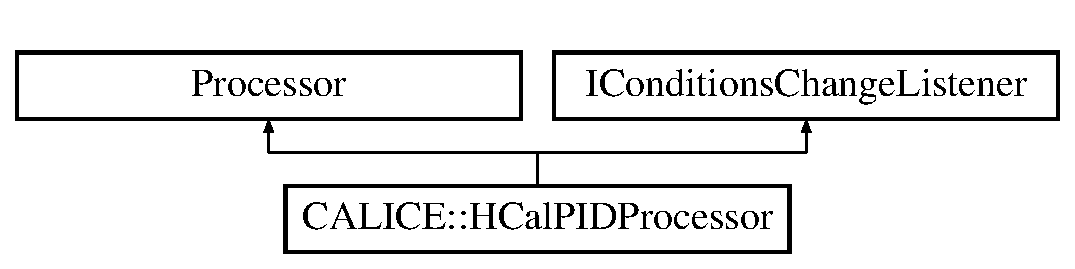
\includegraphics[height=2.000000cm]{classCALICE_1_1HCalPIDProcessor}
\end{center}
\end{figure}
\subsection*{Public Member Functions}
\begin{DoxyCompactItemize}
\item 
{\bf H\-Cal\-P\-I\-D\-Processor} $\ast$ {\bfseries new\-Processor} ()\label{classCALICE_1_1HCalPIDProcessor_a166876f43ec7460b93882ba213d0cda2}

\item 
virtual void {\bfseries init} ()\label{classCALICE_1_1HCalPIDProcessor_a04c4550bdb0d8c12c76b682b37040e51}

\item 
virtual void {\bfseries process\-Run\-Header} (L\-C\-Run\-Header $\ast$)\label{classCALICE_1_1HCalPIDProcessor_ac2e967d5379413aba6e11fa757cb7e06}

\item 
virtual void {\bfseries process\-Event} (lcio\-::\-L\-C\-Event $\ast$)\label{classCALICE_1_1HCalPIDProcessor_ae41234eddfd428a90e4cf192ce2d03e3}

\item 
virtual void {\bfseries end} ()\label{classCALICE_1_1HCalPIDProcessor_a8f03caf555f25eb7bc4171a6c6724253}

\item 
virtual void {\bf conditions\-Changed} (L\-C\-Collection $\ast$col)
\end{DoxyCompactItemize}


\subsection{Detailed Description}
Processor to select (or veto) events from H\-Cal testbeam in P\-S T9 with the particles requested by the user. The steering parameters 'Particle' and 'Veto' define the particle species and if the particle will be selected or vetoed. The selection is based on the information given by Cherenkov counters A and B. In case the selection is not suitable for the requested particle, a warning is printed.

\begin{DoxyAuthor}{Author}
Bruno Lenzi {\tt Bruno.\-Lenzi@cern.\-ch} 
\end{DoxyAuthor}
\begin{DoxyDate}{Date}
Feb 2011 
\end{DoxyDate}


\subsection{Member Function Documentation}
\index{C\-A\-L\-I\-C\-E\-::\-H\-Cal\-P\-I\-D\-Processor@{C\-A\-L\-I\-C\-E\-::\-H\-Cal\-P\-I\-D\-Processor}!conditions\-Changed@{conditions\-Changed}}
\index{conditions\-Changed@{conditions\-Changed}!CALICE::HCalPIDProcessor@{C\-A\-L\-I\-C\-E\-::\-H\-Cal\-P\-I\-D\-Processor}}
\subsubsection[{conditions\-Changed}]{\setlength{\rightskip}{0pt plus 5cm}void C\-A\-L\-I\-C\-E\-::\-H\-Cal\-P\-I\-D\-Processor\-::conditions\-Changed (
\begin{DoxyParamCaption}
\item[{L\-C\-Collection $\ast$}]{col}
\end{DoxyParamCaption}
)\hspace{0.3cm}{\ttfamily [virtual]}}\label{classCALICE_1_1HCalPIDProcessor_ae713feea6d93d385796c2d2bf2919670}
Callback function for the condition changes 

The documentation for this class was generated from the following files\-:\begin{DoxyCompactItemize}
\item 
/nfs/dust/ilc/user/marquezh/\-Calice\-Soft\-\_\-w\-\_\-\-I\-L\-C\-Soft\-\_\-v02-\/03-\/02/calice\-\_\-analysis/addon\-Procs/include/H\-Cal\-P\-I\-D\-Processor.\-hh\item 
/nfs/dust/ilc/user/marquezh/\-Calice\-Soft\-\_\-w\-\_\-\-I\-L\-C\-Soft\-\_\-v02-\/03-\/02/calice\-\_\-analysis/addon\-Procs/src/H\-Cal\-P\-I\-D\-Processor.\-cc\end{DoxyCompactItemize}

\section{Hcal\-T\-M\-V\-A\-Processor Class Reference}
\label{classHcalTMVAProcessor}\index{Hcal\-T\-M\-V\-A\-Processor@{Hcal\-T\-M\-V\-A\-Processor}}
Inheritance diagram for Hcal\-T\-M\-V\-A\-Processor\-:\begin{figure}[H]
\begin{center}
\leavevmode
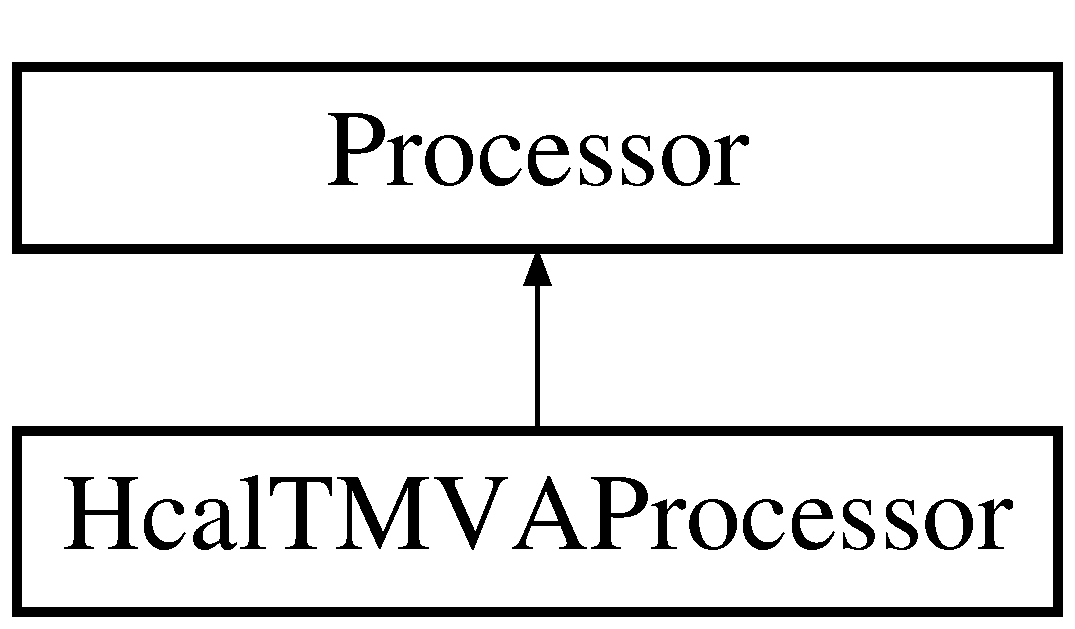
\includegraphics[height=2.000000cm]{classHcalTMVAProcessor}
\end{center}
\end{figure}
\subsection*{Public Member Functions}
\begin{DoxyCompactItemize}
\item 
{\bf Hcal\-T\-M\-V\-A\-Processor} $\ast$ {\bfseries new\-Processor} ()\label{classHcalTMVAProcessor_a349bd1bb9e3a76bcb1eb140f36263859}

\item 
virtual void {\bfseries init} ()\label{classHcalTMVAProcessor_a3a5c09ecf812c886e905ebdc1446ce58}

\item 
virtual void {\bfseries process\-Event} (L\-C\-Event $\ast$)\label{classHcalTMVAProcessor_a4676ff5e437b9545fbecc26c685cfdc9}

\item 
virtual void {\bfseries end} ()\label{classHcalTMVAProcessor_a40f44f94285655cdaf2c42b84eebeaf1}

\end{DoxyCompactItemize}
\subsection*{Protected Member Functions}
\begin{DoxyCompactItemize}
\item 
int {\bfseries cellsize} (int cellid, bool coarse=false)\label{classHcalTMVAProcessor_a22f18ae83004fa9cff45d4eb94ef978b}

\item 
int {\bfseries get\-Marina\-Shower\-Start\-Hcal\-Layer} (L\-C\-Event $\ast$evt, std\-::string shower\-Start\-Col\-Name)\label{classHcalTMVAProcessor_a12c68b7b1c5c921f12de723e41679fa7}

\item 
bool {\bfseries tbtrack\-Loop} (L\-C\-Event $\ast$evt)\label{classHcalTMVAProcessor_ad9528c31a4609b9589014de808134be8}

\item 
void {\bfseries fill\-Root\-Tree} (L\-C\-Event $\ast$evt)\label{classHcalTMVAProcessor_ab9e9661d462cfcd18e7f3d03a4225ea3}

\item 
void {\bfseries T\-M\-V\-A\-Classification} (std\-::string T\-M\-V\-A\-Method\-Name, std\-::string signal\-File\-Name, std\-::string background\-File\-Name, float signal\-Weight, float background\-Weight, std\-::string argument\-For\-Prepare\-Training\-And\-Test\-Tree, std\-::string argument\-For\-Book\-Method)\label{classHcalTMVAProcessor_ab8d2344c572a257e79a032565469849a}

\item 
void {\bfseries T\-M\-V\-A\-Classification\-Application} (std\-::string T\-M\-V\-A\-Method\-Name, std\-::string signal\-File\-Name)\label{classHcalTMVAProcessor_a90d0bc5de7db0722b39cbef51e9dacf8}

\end{DoxyCompactItemize}
\subsection*{Protected Attributes}
\begin{DoxyCompactItemize}
\item 
std\-::string {\bfseries \-\_\-shower\-Start\-Col\-Name}\label{classHcalTMVAProcessor_a828711ef10b4b4556e1650148fdddb56}

\item 
std\-::string {\bfseries \-\_\-ptf\-Track\-Col\-Name}\label{classHcalTMVAProcessor_a866284ca5765034888614bf32ee3a8b5}

\item 
std\-::string {\bfseries \-\_\-hcal\-Col\-Name}\label{classHcalTMVAProcessor_ab91c0aefa8371bb9fea28884413572cf}

\item 
std\-::string {\bfseries \-\_\-ecal\-Col\-Name}\label{classHcalTMVAProcessor_aaf7d811967d03a8b61bd5ca589a0b6a5}

\item 
std\-::string {\bfseries \-\_\-fex\-Track\-Col\-Name}\label{classHcalTMVAProcessor_aa52a884dc3d852f83dd10c0db7b666fe}

\item 
std\-::string {\bfseries \-\_\-fey\-Track\-Col\-Name}\label{classHcalTMVAProcessor_acf4b95a70aa0818757a9dabb70d911dc}

\item 
bool {\bfseries \-\_\-\-Fill\-Root\-Tree}\label{classHcalTMVAProcessor_a9869466d9a7ab2657b00ac02bcda13d4}

\item 
bool {\bfseries \-\_\-\-T\-M\-V\-A\-\_\-\-Training}\label{classHcalTMVAProcessor_a0c790893fd157dd495ed4bd2f7e599a5}

\item 
bool {\bfseries \-\_\-\-T\-M\-V\-A\-\_\-\-Analysis}\label{classHcalTMVAProcessor_a5c0440c4c0f66f41bb5b6a9d21395f11}

\item 
float {\bfseries \-\_\-signal\-Weight}\label{classHcalTMVAProcessor_a8878e5e96b8cf447eb762ff4046ae402}

\item 
float {\bfseries \-\_\-background\-Weight}\label{classHcalTMVAProcessor_a7c44771323a9a99aa8ce5bd9a3c495a4}

\item 
std\-::string {\bfseries \-\_\-\-T\-M\-V\-A\-\_\-\-Method}\label{classHcalTMVAProcessor_a29578e096e86d3f96bb45d235d15323d}

\item 
std\-::string {\bfseries \-\_\-\-T\-M\-V\-A\-\_\-\-Training\-\_\-\-Signal\-File}\label{classHcalTMVAProcessor_a23b46bc83b036cf7f30d9cb97b285944}

\item 
std\-::string {\bfseries \-\_\-\-T\-M\-V\-A\-\_\-\-Training\-\_\-\-Background\-File}\label{classHcalTMVAProcessor_a99d2e077eceb739619f6a96980f6760c}

\item 
std\-::string {\bfseries \-\_\-\-T\-M\-V\-A\-\_\-\-Analysis\-\_\-\-Signal\-File}\label{classHcalTMVAProcessor_ae02107fea53a584976f0410b6736b334}

\item 
std\-::string {\bfseries \-\_\-argument\-For\-Prepare\-Training\-And\-Test\-Tree}\label{classHcalTMVAProcessor_a017d9bd4421477da408429969bc864f6}

\item 
std\-::string {\bfseries \-\_\-argument\-For\-Book\-Method}\label{classHcalTMVAProcessor_a1ec4a723499d288dbe4e73d07d4071c7}

\item 
float {\bfseries \-\_\-fx\-Trk\-At\-Hcal\-Front}\label{classHcalTMVAProcessor_a7ad14a383211affa5f97b60f18f3a41e}

\item 
float {\bfseries \-\_\-fy\-Trk\-At\-Hcal\-Front}\label{classHcalTMVAProcessor_ab7936148a25f097df87ca558b3abc106}

\item 
std\-::string {\bfseries \-\_\-mapping\-Processor\-Name}\label{classHcalTMVAProcessor_a52850d454438baf9ff1523ffde25191a}

\item 
const C\-A\-L\-I\-C\-E\-::\-Ahc\-Mapper $\ast$ {\bfseries \-\_\-mapper}\label{classHcalTMVAProcessor_a16047af3976807c609a9e91816662764}

\item 
std\-::string {\bfseries \-\_\-root\-File\-Name}\label{classHcalTMVAProcessor_a5e07d08f6ceaa0a14d712d05b93bb2bf}

\item 
std\-::string {\bfseries \-\_\-root\-File\-Mode}\label{classHcalTMVAProcessor_a8dfa042a0a07fa7122b99e8654cc3743}

\item 
T\-File $\ast$ {\bfseries \-\_\-root\-File}\label{classHcalTMVAProcessor_aabc121d4b37a5732a333b3ece61f5868}

\item 
T\-Tree $\ast$ {\bfseries \-\_\-root\-Tree}\label{classHcalTMVAProcessor_a2c4856e701ee9b82e8bffe84e84ac020}

\item 
float {\bfseries \-\_\-energy\-Sum}\label{classHcalTMVAProcessor_a00bc9323d52765ce8d2ab4d4b2a6d48e}

\item 
float {\bfseries \-\_\-energy1\-Momentum}\label{classHcalTMVAProcessor_a3b52255ba9b63b79104ffe8b1ecc7421}

\item 
float {\bfseries \-\_\-energy2\-Momentum}\label{classHcalTMVAProcessor_a42ab7b04ad9c379e7fec2205e8136f0d}

\item 
float {\bfseries \-\_\-energy3\-Momentum}\label{classHcalTMVAProcessor_a82308de405661fa309717629b2e28cef}

\item 
float {\bfseries \-\_\-energy\-Ratio}\label{classHcalTMVAProcessor_a30c123fdb9ec6ec83325426a8e7c300f}

\item 
float {\bfseries \-\_\-\-R90\-\_\-hits}\label{classHcalTMVAProcessor_a1333659172590a47aeec97c5dffbfebb}

\item 
float {\bfseries \-\_\-\-N90ratio\-N}\label{classHcalTMVAProcessor_ab4b965bab5e25b3f61f18228613ad7cb}

\item 
float {\bfseries \-\_\-hits\-Mean}\label{classHcalTMVAProcessor_a173a05b0ad67e93838bcdcb68d050622}

\item 
float {\bfseries \-\_\-energy\-Density}\label{classHcalTMVAProcessor_a397d6fba47101360c617b11826ee83f9}

\item 
int {\bfseries \-\_\-layer\-Max\-Diff\-Start}\label{classHcalTMVAProcessor_a6f6692cd1c48be72ca7278b8254cf83d}

\item 
int {\bfseries \-\_\-start\-Layer}\label{classHcalTMVAProcessor_aabb429e5a6a10496999dda602b541006}

\item 
int {\bfseries \-\_\-n\-Layer\-Max\-Energy}\label{classHcalTMVAProcessor_a9fadcc3533a11de7aabcdf1a3e42612f}

\item 
T\-H1\-F $\ast$ {\bfseries \-\_\-h\-Long}\label{classHcalTMVAProcessor_af3334ea5f23a41a21e77968c72b79b0f}

\item 
T\-H1\-F $\ast$ {\bfseries \-\_\-h\-Long\-\_\-from\-Shower\-Start}\label{classHcalTMVAProcessor_a3b67b4268924aa76cc593085f3a3bc57}

\item 
T\-H1\-F $\ast$ {\bfseries \-\_\-h\-Energy\-Sum}\label{classHcalTMVAProcessor_a4f87d18c0692f5df7320ae4372f8323a}

\item 
T\-H1\-F $\ast$ {\bfseries \-\_\-h\-Num\-Hits}\label{classHcalTMVAProcessor_abe950cfbfb7692ab9a0eff9ce1b13fe4}

\item 
T\-H1\-F $\ast$ {\bfseries \-\_\-h\-Shower\-Start}\label{classHcalTMVAProcessor_af14572f4de0c74e68e9889a135794241}

\item 
T\-H1\-F $\ast$ {\bfseries \-\_\-h\-Layer\-Max\-Energy}\label{classHcalTMVAProcessor_a43a01c577c5ffcea6ac03c4582403a45}

\item 
T\-H1\-F $\ast$ {\bfseries \-\_\-h\-Num\-Hits\-Per\-Layer}\label{classHcalTMVAProcessor_a927053a0e53266124e864d43b0545f79}

\item 
T\-H1\-F $\ast$ {\bfseries \-\_\-h\-Hit\-Energy}\label{classHcalTMVAProcessor_a8a652a8351094ade96b56b520c4ae461}

\item 
T\-H1\-F $\ast$ {\bfseries \-\_\-h\-Cog\-X}\label{classHcalTMVAProcessor_a59c2d88635f53f23f19b4f8ac0dbaa9d}

\item 
T\-H1\-F $\ast$ {\bfseries \-\_\-h\-Cog\-Y}\label{classHcalTMVAProcessor_aee553e8c73afc261adb0a1e407efd027}

\item 
T\-H1\-F $\ast$ {\bfseries \-\_\-h\-Trk\-X\-Slope}\label{classHcalTMVAProcessor_ad151e361f63f5508f974eeac8ebed55e}

\item 
T\-H1\-F $\ast$ {\bfseries \-\_\-h\-Trk\-X\-Offset}\label{classHcalTMVAProcessor_a64939191b4e6fbb6be87f4bfa928c38c}

\item 
T\-H1\-F $\ast$ {\bfseries \-\_\-h\-Trk\-X\-At\-Hcal\-Front}\label{classHcalTMVAProcessor_aded67ef40132ed0ff2c1470861430f8e}

\item 
T\-H1\-F $\ast$ {\bfseries \-\_\-h\-Trk\-Y\-Slope}\label{classHcalTMVAProcessor_a17c2a4a3a32b2a67fba024e3d284d4d4}

\item 
T\-H1\-F $\ast$ {\bfseries \-\_\-h\-Trk\-Y\-Offset}\label{classHcalTMVAProcessor_af8695ab9ecdd282d0a94669184229c3e}

\item 
T\-H1\-F $\ast$ {\bfseries \-\_\-h\-Trk\-Y\-At\-Hcal\-Front}\label{classHcalTMVAProcessor_a5ade5d7d0c9764a6e787ab77189146b1}

\end{DoxyCompactItemize}


The documentation for this class was generated from the following files\-:\begin{DoxyCompactItemize}
\item 
/nfs/dust/ilc/user/marquezh/\-Calice\-Soft\-\_\-w\-\_\-\-I\-L\-C\-Soft\-\_\-v02-\/03-\/02/calice\-\_\-analysis/addon\-Procs/include/Hcal\-T\-M\-V\-A\-Processor.\-hh\item 
/nfs/dust/ilc/user/marquezh/\-Calice\-Soft\-\_\-w\-\_\-\-I\-L\-C\-Soft\-\_\-v02-\/03-\/02/calice\-\_\-analysis/addon\-Procs/src/Hcal\-T\-M\-V\-A\-Processor.\-cc\end{DoxyCompactItemize}

\section{Hcal\-Track2\-Root\-Tree Class Reference}
\label{classHcalTrack2RootTree}\index{Hcal\-Track2\-Root\-Tree@{Hcal\-Track2\-Root\-Tree}}
Inheritance diagram for Hcal\-Track2\-Root\-Tree\-:\begin{figure}[H]
\begin{center}
\leavevmode
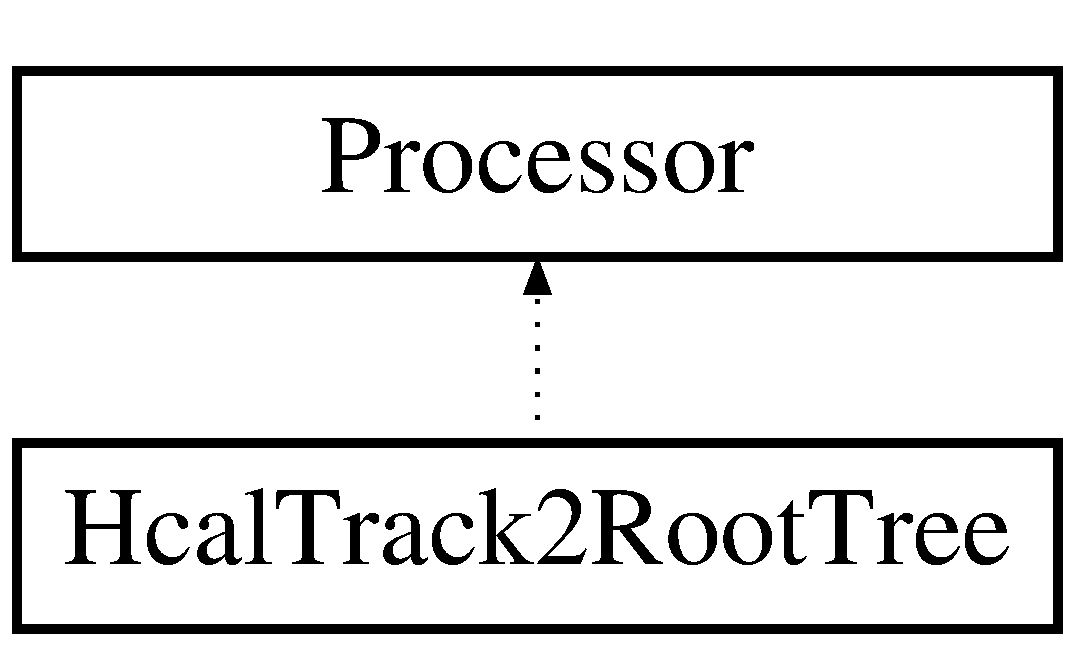
\includegraphics[height=2.000000cm]{classHcalTrack2RootTree}
\end{center}
\end{figure}
\subsection*{Classes}
\begin{DoxyCompactItemize}
\item 
struct {\bf Event\-Tracks}
\end{DoxyCompactItemize}
\subsection*{Public Member Functions}
\begin{DoxyCompactItemize}
\item 
marlin\-::\-Processor $\ast$ {\bfseries new\-Processor} ()\label{classHcalTrack2RootTree_ad456236ad38e9e2c1be0a5a2eac93874}

\item 
virtual void {\bf init} ()
\item 
virtual void {\bf process\-Run\-Header} (L\-C\-Run\-Header $\ast$run)
\item 
virtual void {\bf process\-Event} (L\-C\-Event $\ast$evt)
\item 
virtual void {\bfseries check} (L\-C\-Event $\ast$evt)\label{classHcalTrack2RootTree_a29f5c20d6ec66e5f6b4921bdaa2278d4}

\item 
virtual void {\bf end} ()
\end{DoxyCompactItemize}
\subsection*{Protected Member Functions}
\begin{DoxyCompactItemize}
\item 
virtual Double\-\_\-t {\bfseries get\-Sum\-Of\-Calo\-Hits} (E\-V\-E\-N\-T\-::\-L\-C\-Event $\ast$evt, std\-::string \&collection\-Name)\label{classHcalTrack2RootTree_ae11e481bdb20b591aee8c8a1ef49ab4b}

\end{DoxyCompactItemize}
\subsection*{Protected Attributes}
\begin{DoxyCompactItemize}
\item 
std\-::string {\bfseries \-\_\-lcc\-Cluster}\label{classHcalTrack2RootTree_a1071b5e6d3571ee04bc4c5ee597733b8}

\item 
std\-::string {\bfseries \-\_\-lcc\-Emc\-Calo\-Hits}\label{classHcalTrack2RootTree_a271aa3052901b369fabe54eddf6fb07d}

\item 
std\-::string {\bfseries \-\_\-lcc\-Ahc\-Calo\-Hits}\label{classHcalTrack2RootTree_a0d7cddb36e953cbc60ef5a9f79aa1048}

\item 
std\-::string {\bfseries \-\_\-lcc\-Tcmt\-Calo\-Hits}\label{classHcalTrack2RootTree_a4ab495ec4a37c4128b48912a40991208}

\item 
std\-::string {\bfseries \-\_\-root\-File\-Name}\label{classHcalTrack2RootTree_ac16f4524edd566e28cb5658c14005586}

\item 
std\-::string {\bfseries \-\_\-root\-Tree\-Name}\label{classHcalTrack2RootTree_a0c0752c793010bbab56dac4fe361434c}

\item 
T\-File $\ast$ {\bfseries \-\_\-root\-File}\label{classHcalTrack2RootTree_a0aa2b92a9093cece4b2240f61f51e3d2}

\item 
T\-Tree $\ast$ {\bfseries \-\_\-tree}\label{classHcalTrack2RootTree_a38faf7c09ec870d47739f8388bae8dd8}

\item 
struct \\*
{\bf Hcal\-Track2\-Root\-Tree\-::\-Event\-Tracks} {\bfseries \-\_\-event}\label{classHcalTrack2RootTree_a3567110cb3b30bbbb0bb7ecc3fe260f8}

\end{DoxyCompactItemize}


\subsection{Member Function Documentation}
\index{Hcal\-Track2\-Root\-Tree@{Hcal\-Track2\-Root\-Tree}!end@{end}}
\index{end@{end}!HcalTrack2RootTree@{Hcal\-Track2\-Root\-Tree}}
\subsubsection[{end}]{\setlength{\rightskip}{0pt plus 5cm}void Hcal\-Track2\-Root\-Tree\-::end (
\begin{DoxyParamCaption}
{}
\end{DoxyParamCaption}
)\hspace{0.3cm}{\ttfamily [virtual]}}\label{classHcalTrack2RootTree_a9fcb338340b84484e9c81619d5a679ab}
Called after data processing for clean up. \index{Hcal\-Track2\-Root\-Tree@{Hcal\-Track2\-Root\-Tree}!init@{init}}
\index{init@{init}!HcalTrack2RootTree@{Hcal\-Track2\-Root\-Tree}}
\subsubsection[{init}]{\setlength{\rightskip}{0pt plus 5cm}void Hcal\-Track2\-Root\-Tree\-::init (
\begin{DoxyParamCaption}
{}
\end{DoxyParamCaption}
)\hspace{0.3cm}{\ttfamily [virtual]}}\label{classHcalTrack2RootTree_ae7829c016e9a860d8fa93c232791b56c}
Called at the begin of the job before anything is read. Use to initialize the processor, e.\-g. book histograms. \index{Hcal\-Track2\-Root\-Tree@{Hcal\-Track2\-Root\-Tree}!process\-Event@{process\-Event}}
\index{process\-Event@{process\-Event}!HcalTrack2RootTree@{Hcal\-Track2\-Root\-Tree}}
\subsubsection[{process\-Event}]{\setlength{\rightskip}{0pt plus 5cm}void Hcal\-Track2\-Root\-Tree\-::process\-Event (
\begin{DoxyParamCaption}
\item[{L\-C\-Event $\ast$}]{evt}
\end{DoxyParamCaption}
)\hspace{0.3cm}{\ttfamily [virtual]}}\label{classHcalTrack2RootTree_afe26e70d3e12edabd0a8117295879b80}
Called for every event -\/ the working horse. \index{Hcal\-Track2\-Root\-Tree@{Hcal\-Track2\-Root\-Tree}!process\-Run\-Header@{process\-Run\-Header}}
\index{process\-Run\-Header@{process\-Run\-Header}!HcalTrack2RootTree@{Hcal\-Track2\-Root\-Tree}}
\subsubsection[{process\-Run\-Header}]{\setlength{\rightskip}{0pt plus 5cm}void Hcal\-Track2\-Root\-Tree\-::process\-Run\-Header (
\begin{DoxyParamCaption}
\item[{L\-C\-Run\-Header $\ast$}]{run}
\end{DoxyParamCaption}
)\hspace{0.3cm}{\ttfamily [virtual]}}\label{classHcalTrack2RootTree_a66302b201e51a169f02f589b9dee6236}
Called for every run. 

The documentation for this class was generated from the following files\-:\begin{DoxyCompactItemize}
\item 
/nfs/dust/ilc/user/marquezh/\-Calice\-Soft\-\_\-w\-\_\-\-I\-L\-C\-Soft\-\_\-v02-\/03-\/02/calice\-\_\-analysis/addon\-Procs/include/Hcal\-Track2\-Root\-Tree.\-hh\item 
/nfs/dust/ilc/user/marquezh/\-Calice\-Soft\-\_\-w\-\_\-\-I\-L\-C\-Soft\-\_\-v02-\/03-\/02/calice\-\_\-analysis/addon\-Procs/src/Hcal\-Track2\-Root\-Tree.\-cc\end{DoxyCompactItemize}

\section{H\-Cal\-Tracking\-N\-N\-Processor\-:\-:H\-Cal\-Tracked\-Hit Class Reference}
\label{classHCalTrackingNNProcessor_1_1HCalTrackedHit}\index{H\-Cal\-Tracking\-N\-N\-Processor\-::\-H\-Cal\-Tracked\-Hit@{H\-Cal\-Tracking\-N\-N\-Processor\-::\-H\-Cal\-Tracked\-Hit}}


{\ttfamily \#include $<$Hcal\-Tracking\-N\-N.\-hh$>$}

\subsection*{Public Member Functions}
\begin{DoxyCompactItemize}
\item 
{\bfseries H\-Cal\-Tracked\-Hit} (E\-V\-E\-N\-T\-::\-Calorimeter\-Hit $\ast$h)\label{classHCalTrackingNNProcessor_1_1HCalTrackedHit_afb2399747fbd27bdb23cd2f7cca9693a}

\item 
E\-V\-E\-N\-T\-::\-Calorimeter\-Hit $\ast$ {\bfseries get\-Hit} ()\label{classHCalTrackingNNProcessor_1_1HCalTrackedHit_ac05da13ef1a516b815bd06597c640cae}

\item 
void {\bfseries add\-Neighbour} ({\bf H\-Cal\-Tracked\-Hit} $\ast$h)\label{classHCalTrackingNNProcessor_1_1HCalTrackedHit_a797b4a358484166656c9eb85d5bee3de}

\item 
const std\-::list$<$ {\bf H\-Cal\-Tracked\-Hit} $\ast$ $>$ {\bfseries get\-Neighbours} ()\label{classHCalTrackingNNProcessor_1_1HCalTrackedHit_a8e78d13b8ecf48433ca0a9d96d4f5bb1}

\item 
const unsigned {\bfseries get\-K} ()\label{classHCalTrackingNNProcessor_1_1HCalTrackedHit_ad873e2e7992a314249ae6ea3bba4b1f4}

\item 
const bool {\bfseries is\-Isolated} ()\label{classHCalTrackingNNProcessor_1_1HCalTrackedHit_a9988328d20aa514fc0d8bac745d9078f}

\item 
void {\bfseries set\-Track} (E\-V\-E\-N\-T\-::\-Cluster $\ast$track)\label{classHCalTrackingNNProcessor_1_1HCalTrackedHit_a4954bee012a96567e9e3d7d3dfc01ddb}

\item 
const bool {\bfseries has\-Track} ()\label{classHCalTrackingNNProcessor_1_1HCalTrackedHit_aa2a18fd5aaa2fb7aefa14b94807efff3}

\item 
const E\-V\-E\-N\-T\-::\-Cluster $\ast$ {\bfseries get\-Track} ()\label{classHCalTrackingNNProcessor_1_1HCalTrackedHit_a9d088a7c2bcf5ad3aeeeed748568c210}

\end{DoxyCompactItemize}
\subsection*{Protected Attributes}
\begin{DoxyCompactItemize}
\item 
E\-V\-E\-N\-T\-::\-Calorimeter\-Hit $\ast$ {\bfseries \-\_\-hit}\label{classHCalTrackingNNProcessor_1_1HCalTrackedHit_a256ad292c6ca6640e1930a9150811068}

\item 
std\-::list$<$ {\bf H\-Cal\-Tracked\-Hit} $\ast$ $>$ {\bfseries \-\_\-neighbours}\label{classHCalTrackingNNProcessor_1_1HCalTrackedHit_ae82af8afc010694eed261e0fbf0bebc1}

\item 
E\-V\-E\-N\-T\-::\-Cluster $\ast$ {\bfseries \-\_\-track}\label{classHCalTrackingNNProcessor_1_1HCalTrackedHit_ae36cf46d6ede64087b3f83da3bd97c88}

\end{DoxyCompactItemize}


\subsection{Detailed Description}
Wrapper around the actual Calorimeter\-Hit, s.\-t. we can add additional information like the neighbors 

The documentation for this class was generated from the following file\-:\begin{DoxyCompactItemize}
\item 
/nfs/dust/ilc/user/marquezh/\-Calice\-Soft\-\_\-w\-\_\-\-I\-L\-C\-Soft\-\_\-v02-\/03-\/02/calice\-\_\-analysis/addon\-Procs/include/Hcal\-Tracking\-N\-N.\-hh\end{DoxyCompactItemize}

\section{H\-Cal\-Track\-Filter Class Reference}
\label{classHCalTrackFilter}\index{H\-Cal\-Track\-Filter@{H\-Cal\-Track\-Filter}}
Inheritance diagram for H\-Cal\-Track\-Filter\-:\begin{figure}[H]
\begin{center}
\leavevmode
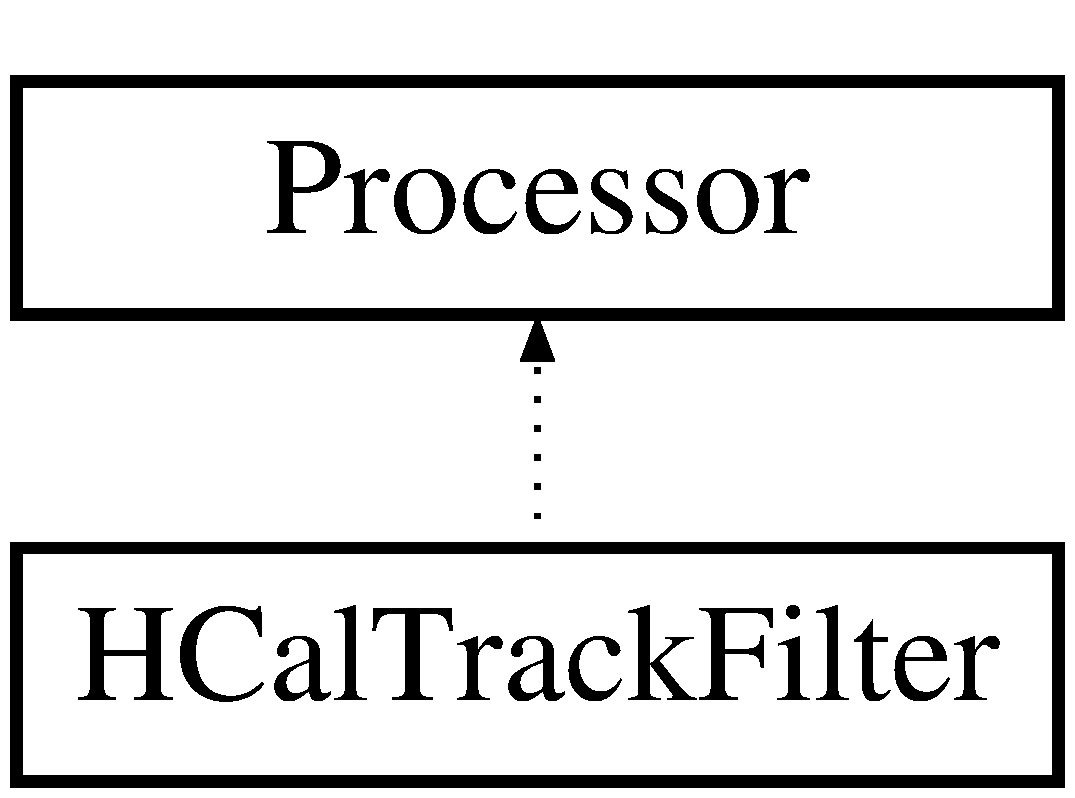
\includegraphics[height=2.000000cm]{classHCalTrackFilter}
\end{center}
\end{figure}
\subsection*{Public Member Functions}
\begin{DoxyCompactItemize}
\item 
marlin\-::\-Processor $\ast$ {\bfseries new\-Processor} ()\label{classHCalTrackFilter_a42fae3a98615aaf4f163401d2156b091}

\item 
virtual void {\bf init} ()
\item 
virtual void {\bf process\-Run\-Header} (L\-C\-Run\-Header $\ast$run)
\item 
virtual void {\bf process\-Event} (L\-C\-Event $\ast$evt)
\item 
virtual void {\bfseries check} (L\-C\-Event $\ast$evt)\label{classHCalTrackFilter_a140c52dc7476c0116033173bea32e589}

\item 
virtual void {\bf end} ()
\end{DoxyCompactItemize}
\subsection*{Protected Member Functions}
\begin{DoxyCompactItemize}
\item 
virtual E\-V\-E\-N\-T\-::\-Cluster $\ast$ {\bfseries filter\-Track\-Hough} (E\-V\-E\-N\-T\-::\-Cluster $\ast$track)\label{classHCalTrackFilter_a212d7686c61f5b50f9ca0364d49eae94}

\item 
void {\bfseries divide\-And\-Check\-Hough\-Space} (int m\-Min, int r\-Min, int m\-Max, int r\-Max)\label{classHCalTrackFilter_a2fe6db1741b034405180f79e07d7b991}

\end{DoxyCompactItemize}
\subsection*{Protected Attributes}
\begin{DoxyCompactItemize}
\item 
std\-::vector$<$ double $>$ {\bfseries \-\_\-hough\-Space\-Binning\-M}\label{classHCalTrackFilter_aca9c7072b7b890c2b5a7e837e5f5aace}

\item 
std\-::vector$<$ double $>$ {\bfseries \-\_\-hough\-Space\-Binning\-T}\label{classHCalTrackFilter_a37d51653b75afd2d49c3b14c7d7f3975}

\item 
std\-::vector$<$ {\bf Hough\-Band} $\ast$ $>$ {\bfseries \-\_\-all\-Hough\-Bands}\label{classHCalTrackFilter_a269b9de68d416296a85513a5055a1de7}

\item 
std\-::vector$<$ {\bf Hough\-Band} $\ast$ $>$ {\bfseries \-\_\-biggest\-Intersection}\label{classHCalTrackFilter_acdc46ed6288b80bdfa02e059d715ad4e}

\item 
int {\bfseries \-\_\-recursive\-Counter}\label{classHCalTrackFilter_a0d0612b016022c9b2ba7f8dd78be9be9}

\item 
C\-A\-L\-I\-C\-E\-::\-Mapped\-Container\\*
$<$ C\-A\-L\-I\-C\-E\-::\-Cell\-Description $>$ $\ast$ {\bfseries \-\_\-cell\-Descriptions}\label{classHCalTrackFilter_a3e0c3d717120ad1db2d78e0799e67d4a}

\item 
std\-::string {\bfseries \-\_\-cell\-Description\-Processor\-Name}\label{classHCalTrackFilter_aba43cb0e3543f152a94c612fef0a5d7d}

\item 
std\-::string {\bfseries \-\_\-lcc\-Track\-Cluster\-Name}\label{classHCalTrackFilter_a2b8f5be022e46d4490deb2145c3ca7f4}

\item 
std\-::string {\bfseries \-\_\-lcc\-Filtered\-Track\-Cluster\-Name}\label{classHCalTrackFilter_a0d282b7afe432306d80bf825f17e90da}

\item 
int {\bfseries \-\_\-min\-Number\-Of\-Hits}\label{classHCalTrackFilter_a2741e0107f22d5591b8a7b113e63e610}

\item 
int {\bfseries \-\_\-max\-Nr\-Rejected\-Hits}\label{classHCalTrackFilter_aa62684492d509b45ff1ac83bc7e66322}

\item 
unsigned {\bfseries \-\_\-stats\-Nr\-Hits\-Rejected}\label{classHCalTrackFilter_a91b9bae7fc736f0f1e34d4c0baaa262d}

\item 
unsigned {\bfseries \-\_\-stats\-Nr\-Tracks\-Rejected}\label{classHCalTrackFilter_abab3e86ca7dabdc8a95007938fdaca26}

\item 
unsigned {\bfseries \-\_\-stats\-Nr\-Events}\label{classHCalTrackFilter_a051a4318eef7a08434d3d97be69f24ee}

\item 
unsigned {\bfseries \-\_\-stats\-Nr\-Tracks}\label{classHCalTrackFilter_a45a6a1ea3ca1bb34d8fa9052d179cae0}

\end{DoxyCompactItemize}


\subsection{Member Function Documentation}
\index{H\-Cal\-Track\-Filter@{H\-Cal\-Track\-Filter}!end@{end}}
\index{end@{end}!HCalTrackFilter@{H\-Cal\-Track\-Filter}}
\subsubsection[{end}]{\setlength{\rightskip}{0pt plus 5cm}void H\-Cal\-Track\-Filter\-::end (
\begin{DoxyParamCaption}
{}
\end{DoxyParamCaption}
)\hspace{0.3cm}{\ttfamily [virtual]}}\label{classHCalTrackFilter_a76efe273651d21a7197df73113ca04cc}
Called after data processing for clean up. \index{H\-Cal\-Track\-Filter@{H\-Cal\-Track\-Filter}!init@{init}}
\index{init@{init}!HCalTrackFilter@{H\-Cal\-Track\-Filter}}
\subsubsection[{init}]{\setlength{\rightskip}{0pt plus 5cm}void H\-Cal\-Track\-Filter\-::init (
\begin{DoxyParamCaption}
{}
\end{DoxyParamCaption}
)\hspace{0.3cm}{\ttfamily [virtual]}}\label{classHCalTrackFilter_a3913b55fc4b34aa6abe6a1f1120f0096}
Called at the begin of the job before anything is read. Use to initialize the processor, e.\-g. book histograms. \index{H\-Cal\-Track\-Filter@{H\-Cal\-Track\-Filter}!process\-Event@{process\-Event}}
\index{process\-Event@{process\-Event}!HCalTrackFilter@{H\-Cal\-Track\-Filter}}
\subsubsection[{process\-Event}]{\setlength{\rightskip}{0pt plus 5cm}void H\-Cal\-Track\-Filter\-::process\-Event (
\begin{DoxyParamCaption}
\item[{L\-C\-Event $\ast$}]{evt}
\end{DoxyParamCaption}
)\hspace{0.3cm}{\ttfamily [virtual]}}\label{classHCalTrackFilter_aec07b7d533c6214c3b02bfc07f89c47b}
Called for every event -\/ the working horse. \index{H\-Cal\-Track\-Filter@{H\-Cal\-Track\-Filter}!process\-Run\-Header@{process\-Run\-Header}}
\index{process\-Run\-Header@{process\-Run\-Header}!HCalTrackFilter@{H\-Cal\-Track\-Filter}}
\subsubsection[{process\-Run\-Header}]{\setlength{\rightskip}{0pt plus 5cm}virtual void H\-Cal\-Track\-Filter\-::process\-Run\-Header (
\begin{DoxyParamCaption}
\item[{L\-C\-Run\-Header $\ast$}]{run}
\end{DoxyParamCaption}
)\hspace{0.3cm}{\ttfamily [inline]}, {\ttfamily [virtual]}}\label{classHCalTrackFilter_a5b3799e2dacbab50c8cec27424bd72be}
Called for every run. 

The documentation for this class was generated from the following files\-:\begin{DoxyCompactItemize}
\item 
/nfs/dust/ilc/user/marquezh/\-Calice\-Soft\-\_\-w\-\_\-\-I\-L\-C\-Soft\-\_\-v02-\/03-\/02/calice\-\_\-analysis/addon\-Procs/include/H\-Cal\-Track\-Filter.\-hh\item 
/nfs/dust/ilc/user/marquezh/\-Calice\-Soft\-\_\-w\-\_\-\-I\-L\-C\-Soft\-\_\-v02-\/03-\/02/calice\-\_\-analysis/addon\-Procs/src/H\-Cal\-Track\-Filter.\-cc\end{DoxyCompactItemize}

\section{H\-Cal\-Tracking\-N\-N\-Processor Class Reference}
\label{classHCalTrackingNNProcessor}\index{H\-Cal\-Tracking\-N\-N\-Processor@{H\-Cal\-Tracking\-N\-N\-Processor}}


{\ttfamily \#include $<$Hcal\-Tracking\-N\-N.\-hh$>$}

Inheritance diagram for H\-Cal\-Tracking\-N\-N\-Processor\-:\begin{figure}[H]
\begin{center}
\leavevmode
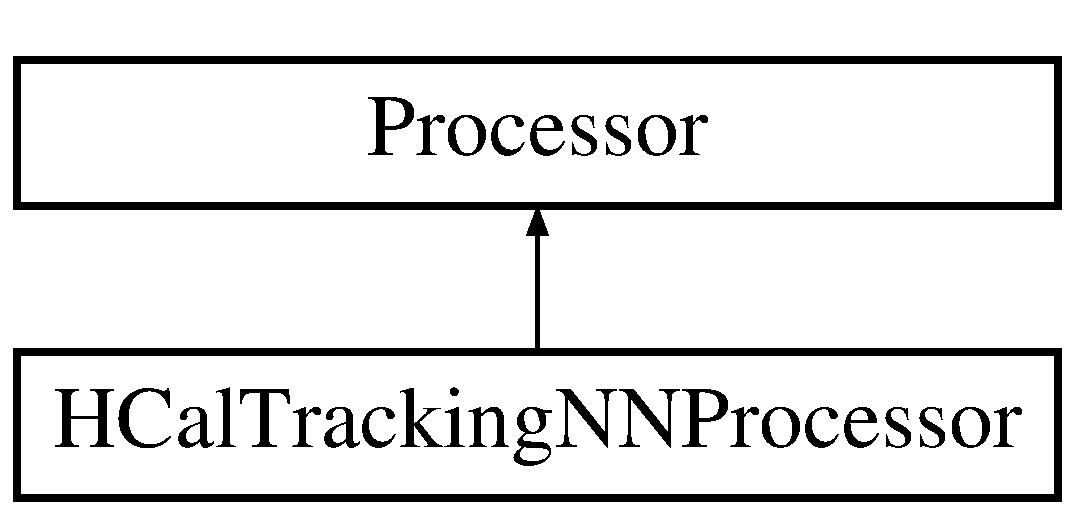
\includegraphics[height=2.000000cm]{classHCalTrackingNNProcessor}
\end{center}
\end{figure}
\subsection*{Classes}
\begin{DoxyCompactItemize}
\item 
class {\bf H\-Cal\-Tracked\-Hit}
\end{DoxyCompactItemize}
\subsection*{Public Member Functions}
\begin{DoxyCompactItemize}
\item 
virtual {\bf $\sim$\-H\-Cal\-Tracking\-N\-N\-Processor} ()
\item 
marlin\-::\-Processor $\ast$ {\bfseries new\-Processor} ()\label{classHCalTrackingNNProcessor_aac4d06e41720579d7f24c0c3835c4519}

\item 
virtual void {\bf init} ()
\item 
virtual void {\bf process\-Run\-Header} (L\-C\-Run\-Header $\ast$run)
\item 
virtual void {\bf process\-Event} (L\-C\-Event $\ast$evt)
\item 
virtual void {\bfseries check} (L\-C\-Event $\ast$evt)\label{classHCalTrackingNNProcessor_a5c6e5cb2aa8ce74d13815641f4d3c0ca}

\item 
virtual void {\bf end} ()
\end{DoxyCompactItemize}
\subsection*{Protected Types}
\begin{DoxyCompactItemize}
\item 
typedef boost\-::unordered\-\_\-map\\*
$<$ unsigned, {\bf H\-Cal\-Tracked\-Hit} $\ast$ $>$ {\bfseries hash\-Map\-Hits\-\_\-t}\label{classHCalTrackingNNProcessor_a53a207437efcb088881b0b46030b6ee3}

\item 
typedef std\-::map$<$ unsigned, \\*
hash\-Map\-Hits\-\_\-t $>$ {\bfseries map\-Hashmap\-Hits\-\_\-t}\label{classHCalTrackingNNProcessor_ac66df3d2b2f2ebc6abb91541b33c8c01}

\end{DoxyCompactItemize}
\subsection*{Protected Member Functions}
\begin{DoxyCompactItemize}
\item 
void {\bf analyze\-Single\-Event} (L\-C\-Collection $\ast$event)
\item 
void {\bfseries set\-Track\-Angle} (E\-V\-E\-N\-T\-::\-Cluster $\ast$track)\label{classHCalTrackingNNProcessor_ac0c71ddc6d42d008977164cbc7a630ca}

\item 
void {\bfseries print\-Status} ()\label{classHCalTrackingNNProcessor_acbc06acf8aa197f8f08564e9c8737488}

\item 
void {\bfseries fill\-Hit\-Map} (L\-C\-Collection $\ast$evt)\label{classHCalTrackingNNProcessor_a26b8b7800790dc7c92f91e760e65060f}

\item 
void {\bfseries count\-Neighbours} ()\label{classHCalTrackingNNProcessor_a5982d56f68096926ba9ffafdba6492d6}

\item 
void {\bfseries find\-Tracks} ()\label{classHCalTrackingNNProcessor_a5616071406e2c134b27708eb8ce79406}

\item 
void {\bfseries clean\-Up} ()\label{classHCalTrackingNNProcessor_a81b64e667dfb82fd618483e7622c1e54}

\item 
E\-V\-E\-N\-T\-::\-Cluster $\ast$ {\bfseries find\-Single\-Track} ({\bf H\-Cal\-Tracked\-Hit} $\ast$first\-Hit)\label{classHCalTrackingNNProcessor_a2d1fa550dd88bd44d8eba2e60e865233}

\item 
void {\bfseries add\-Track} (E\-V\-E\-N\-T\-::\-Cluster $\ast$track)\label{classHCalTrackingNNProcessor_af2f77e426981c935018fdbdeb70ebe78}

\item 
int {\bfseries get\-Track\-Layer\-Length} (E\-V\-E\-N\-T\-::\-Cluster $\ast$track)\label{classHCalTrackingNNProcessor_adfa6baef7083471ec1bd9d9eb224a825}

\item 
void {\bfseries delete\-Track} (E\-V\-E\-N\-T\-::\-Cluster $\ast$track)\label{classHCalTrackingNNProcessor_a51dd0aca10d6d787fb5d587e2169cb28}

\end{DoxyCompactItemize}
\subsection*{Protected Attributes}
\begin{DoxyCompactItemize}
\item 
C\-A\-L\-I\-C\-E\-::\-Mapped\-Container\\*
$<$ C\-A\-L\-I\-C\-E\-::\-Cell\-Description $>$ $\ast$ {\bfseries \-\_\-cell\-Descriptions}\label{classHCalTrackingNNProcessor_ab99634a7a2381df856fc03dfc9a14746}

\item 
C\-A\-L\-I\-C\-E\-::\-Mapped\-Container\\*
$<$ C\-A\-L\-I\-C\-E\-::\-Cell\-Neighbours $>$ $\ast$ {\bfseries \-\_\-cell\-Neighbours}\label{classHCalTrackingNNProcessor_a98c62324557cb29ccee95c4732a7ed8e}

\item 
std\-::string {\bfseries \-\_\-cell\-Description\-Processor\-Name}\label{classHCalTrackingNNProcessor_af925574ee11b92a6cb68e40a54847256}

\item 
std\-::string {\bfseries \-\_\-cell\-Neighbour\-Processor\-Name}\label{classHCalTrackingNNProcessor_a3b30cd8461ceb63cd4eaa06f72fce463}

\item 
std\-::string {\bfseries \-\_\-lcc\-Calorimeter\-Hits\-Name}\label{classHCalTrackingNNProcessor_acd02724e047ef7709b106763df328c61}

\item 
std\-::string {\bfseries \-\_\-lcc\-Track\-Cluster\-Out\-Name}\label{classHCalTrackingNNProcessor_a552a2ae2175dd0b2d25ad7614bb1b13d}

\item 
int {\bfseries \-\_\-max\-Gap\-Size}\label{classHCalTrackingNNProcessor_a5727d97f52617147f667c5687c54c4e5}

\item 
int {\bfseries \-\_\-min\-Track\-Length}\label{classHCalTrackingNNProcessor_a50f6eb654cede963c96bfc3595409ff1}

\item 
double {\bfseries \-\_\-max\-Track\-Gap\-Ratio}\label{classHCalTrackingNNProcessor_a185318818a7bf21116b05d1ed05230db}

\item 
map\-Hashmap\-Hits\-\_\-t {\bfseries \-\_\-hits}\label{classHCalTrackingNNProcessor_a5454f68399fd7edce4d63ef7d7ff2b45}

\item 
I\-M\-P\-L\-::\-L\-C\-Collection\-Vec $\ast$ {\bfseries \-\_\-tracks}\label{classHCalTrackingNNProcessor_af134797b8e36d66d70c760f313d9eed5}

\item 
int {\bfseries \-\_\-stat\-N\-Processed\-Events}\label{classHCalTrackingNNProcessor_aae2cd6cbe12f845cb18666096a4e01ef}

\item 
int {\bfseries \-\_\-stat\-N\-Empty\-Events}\label{classHCalTrackingNNProcessor_a13150263f7ac321c0198379aaae28ad7}

\item 
int {\bfseries \-\_\-stat\-N\-Runs}\label{classHCalTrackingNNProcessor_aaa8fa58d0503315e8e1a8b47bdc86da8}

\item 
int {\bfseries \-\_\-stat\-N\-Tracks}\label{classHCalTrackingNNProcessor_ae5f4d0e1feb52d0e5e6e70151f4b9b11}

\item 
int {\bfseries \-\_\-dbg\-Indent\-Size}\label{classHCalTrackingNNProcessor_aec5a1f7fbd3f4f14fd42e66ec58390cc}

\end{DoxyCompactItemize}
\subsection*{Friends}
\begin{DoxyCompactItemize}
\item 
std\-::ostream \& {\bfseries operator$<$$<$} (std\-::ostream \&out, E\-V\-E\-N\-T\-::\-Cluster $\ast$track)\label{classHCalTrackingNNProcessor_ac878b174fea2efa52f499df6135324b9}

\end{DoxyCompactItemize}


\subsection{Detailed Description}
This marlin processor tries to find tracks in the calorimeter. Currently optimised for the A\-H\-Cal of C\-A\-L\-I\-C\-E.

The algorithm works the following way\-:
\begin{DoxyEnumerate}
\item Check all hits whether they are isolated (e.\-g. have no neighbour hits in the same layer)
\item Take an isolated hit and advance to the next layer. Check, if there is an isolated hit at the same position. If there is\-: join them together to a track.
\item For analysis, the energy distribution for all found tracks is saved. (both total, and per tile) 
\end{DoxyEnumerate}

\subsection{Constructor \& Destructor Documentation}
\index{H\-Cal\-Tracking\-N\-N\-Processor@{H\-Cal\-Tracking\-N\-N\-Processor}!$\sim$\-H\-Cal\-Tracking\-N\-N\-Processor@{$\sim$\-H\-Cal\-Tracking\-N\-N\-Processor}}
\index{$\sim$\-H\-Cal\-Tracking\-N\-N\-Processor@{$\sim$\-H\-Cal\-Tracking\-N\-N\-Processor}!HCalTrackingNNProcessor@{H\-Cal\-Tracking\-N\-N\-Processor}}
\subsubsection[{$\sim$\-H\-Cal\-Tracking\-N\-N\-Processor}]{\setlength{\rightskip}{0pt plus 5cm}H\-Cal\-Tracking\-N\-N\-Processor\-::$\sim$\-H\-Cal\-Tracking\-N\-N\-Processor (
\begin{DoxyParamCaption}
{}
\end{DoxyParamCaption}
)\hspace{0.3cm}{\ttfamily [virtual]}}\label{classHCalTrackingNNProcessor_a33033b8ed04d1f3cceb3bfc96ad709ae}
constructor 

\subsection{Member Function Documentation}
\index{H\-Cal\-Tracking\-N\-N\-Processor@{H\-Cal\-Tracking\-N\-N\-Processor}!analyze\-Single\-Event@{analyze\-Single\-Event}}
\index{analyze\-Single\-Event@{analyze\-Single\-Event}!HCalTrackingNNProcessor@{H\-Cal\-Tracking\-N\-N\-Processor}}
\subsubsection[{analyze\-Single\-Event}]{\setlength{\rightskip}{0pt plus 5cm}void H\-Cal\-Tracking\-N\-N\-Processor\-::analyze\-Single\-Event (
\begin{DoxyParamCaption}
\item[{L\-C\-Collection $\ast$}]{event}
\end{DoxyParamCaption}
)\hspace{0.3cm}{\ttfamily [protected]}}\label{classHCalTrackingNNProcessor_ac418d354d37705957eb80fb1b7c11424}
returns\-: no. of found tracks

does the actual tracking gets called from process\-Event after Trigger / other options have been checked and this event considered to be ok 

Referenced by process\-Event().

\index{H\-Cal\-Tracking\-N\-N\-Processor@{H\-Cal\-Tracking\-N\-N\-Processor}!end@{end}}
\index{end@{end}!HCalTrackingNNProcessor@{H\-Cal\-Tracking\-N\-N\-Processor}}
\subsubsection[{end}]{\setlength{\rightskip}{0pt plus 5cm}void H\-Cal\-Tracking\-N\-N\-Processor\-::end (
\begin{DoxyParamCaption}
{}
\end{DoxyParamCaption}
)\hspace{0.3cm}{\ttfamily [virtual]}}\label{classHCalTrackingNNProcessor_a32156c53787160c372c9ac485fa3b9da}
Called after data processing for clean up. \index{H\-Cal\-Tracking\-N\-N\-Processor@{H\-Cal\-Tracking\-N\-N\-Processor}!init@{init}}
\index{init@{init}!HCalTrackingNNProcessor@{H\-Cal\-Tracking\-N\-N\-Processor}}
\subsubsection[{init}]{\setlength{\rightskip}{0pt plus 5cm}void H\-Cal\-Tracking\-N\-N\-Processor\-::init (
\begin{DoxyParamCaption}
{}
\end{DoxyParamCaption}
)\hspace{0.3cm}{\ttfamily [virtual]}}\label{classHCalTrackingNNProcessor_a489c7c23d1384643705240a06f9b8fb0}
Called at the begin of the job before anything is read. Use to initialize the processor, e.\-g. book histograms. \index{H\-Cal\-Tracking\-N\-N\-Processor@{H\-Cal\-Tracking\-N\-N\-Processor}!process\-Event@{process\-Event}}
\index{process\-Event@{process\-Event}!HCalTrackingNNProcessor@{H\-Cal\-Tracking\-N\-N\-Processor}}
\subsubsection[{process\-Event}]{\setlength{\rightskip}{0pt plus 5cm}void H\-Cal\-Tracking\-N\-N\-Processor\-::process\-Event (
\begin{DoxyParamCaption}
\item[{L\-C\-Event $\ast$}]{evt}
\end{DoxyParamCaption}
)\hspace{0.3cm}{\ttfamily [virtual]}}\label{classHCalTrackingNNProcessor_a2e9dceeccdda57febe1bc8149b62847f}
Called for every event -\/ the working horse.

L\-C\-I\-O input\-: iterates through all events. The tracking algorithm will try to find tracks for each event. 

References analyze\-Single\-Event().

\index{H\-Cal\-Tracking\-N\-N\-Processor@{H\-Cal\-Tracking\-N\-N\-Processor}!process\-Run\-Header@{process\-Run\-Header}}
\index{process\-Run\-Header@{process\-Run\-Header}!HCalTrackingNNProcessor@{H\-Cal\-Tracking\-N\-N\-Processor}}
\subsubsection[{process\-Run\-Header}]{\setlength{\rightskip}{0pt plus 5cm}void H\-Cal\-Tracking\-N\-N\-Processor\-::process\-Run\-Header (
\begin{DoxyParamCaption}
\item[{L\-C\-Run\-Header $\ast$}]{run}
\end{DoxyParamCaption}
)\hspace{0.3cm}{\ttfamily [virtual]}}\label{classHCalTrackingNNProcessor_a969e1d99c96d6220ba06324113295d35}
Called for every run. 

The documentation for this class was generated from the following files\-:\begin{DoxyCompactItemize}
\item 
/nfs/dust/ilc/user/marquezh/\-Calice\-Soft\-\_\-w\-\_\-\-I\-L\-C\-Soft\-\_\-v02-\/03-\/02/calice\-\_\-analysis/addon\-Procs/include/Hcal\-Tracking\-N\-N.\-hh\item 
/nfs/dust/ilc/user/marquezh/\-Calice\-Soft\-\_\-w\-\_\-\-I\-L\-C\-Soft\-\_\-v02-\/03-\/02/calice\-\_\-analysis/addon\-Procs/src/Hcal\-Tracking\-N\-N.\-cc\end{DoxyCompactItemize}

\section{C\-A\-L\-I\-C\-E\-:\-:Hit\-Classification\-Processor Class Reference}
\label{classCALICE_1_1HitClassificationProcessor}\index{C\-A\-L\-I\-C\-E\-::\-Hit\-Classification\-Processor@{C\-A\-L\-I\-C\-E\-::\-Hit\-Classification\-Processor}}


Processor finds detached hits in event and gives 2 collections\-: Detached hits and event w/o detached hits.  




{\ttfamily \#include $<$Hit\-Classification\-Processor.\-hh$>$}

Inheritance diagram for C\-A\-L\-I\-C\-E\-:\-:Hit\-Classification\-Processor\-:\begin{figure}[H]
\begin{center}
\leavevmode
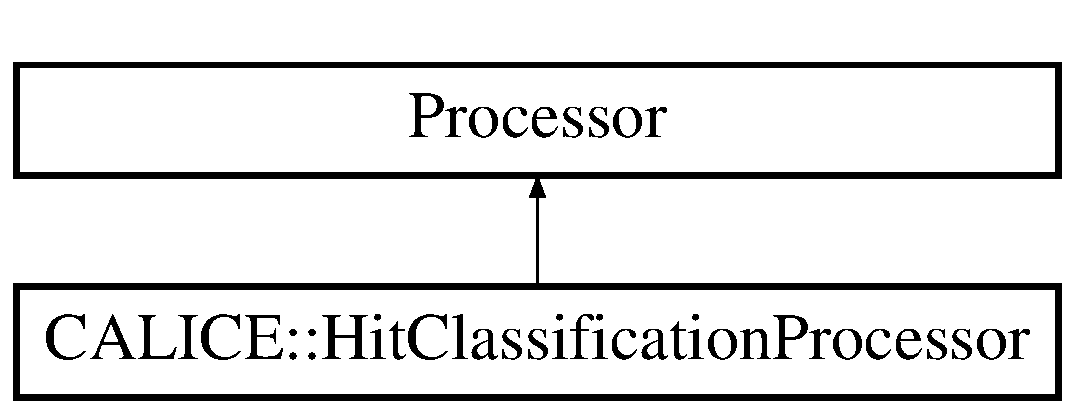
\includegraphics[height=2.000000cm]{classCALICE_1_1HitClassificationProcessor}
\end{center}
\end{figure}
\subsection*{Public Member Functions}
\begin{DoxyCompactItemize}
\item 
virtual Processor $\ast$ {\bfseries new\-Processor} ()\label{classCALICE_1_1HitClassificationProcessor_a955e933140dd61e6872006ae87b03dbb}

\item 
virtual void {\bfseries init} ()\label{classCALICE_1_1HitClassificationProcessor_aa32a1e394d3603fb4f3bb5f53e6ed763}

\item 
virtual void {\bfseries process\-Run\-Header} (L\-C\-Run\-Header $\ast$run)\label{classCALICE_1_1HitClassificationProcessor_a5c3bcde173f33d807daefb887bbae3b9}

\item 
virtual void {\bfseries process\-Event} (L\-C\-Event $\ast$evt)\label{classCALICE_1_1HitClassificationProcessor_ad4f0b48757846cfd3124daac76b60e5a}

\item 
virtual void {\bfseries check} (L\-C\-Event $\ast$evt)\label{classCALICE_1_1HitClassificationProcessor_a96bed7213ac43218cc0d4244e2080820}

\item 
virtual void {\bfseries end} ()\label{classCALICE_1_1HitClassificationProcessor_ab2715b8619f2fa7209df2a3a8032ff4e}

\item 
virtual void {\bfseries print\-Parameters} ()\label{classCALICE_1_1HitClassificationProcessor_addd70f96ba47f8df876699d21e5425ff}

\end{DoxyCompactItemize}
\subsection*{Protected Attributes}
\begin{DoxyCompactItemize}
\item 
std\-::string {\bfseries \-\_\-hit\-In\-Col\-Name}\label{classCALICE_1_1HitClassificationProcessor_a9728f3e9e72130b73d912cf0c50f67fd}

\item 
std\-::string {\bfseries \-\_\-hit\-Relations\-Col\-Name}\label{classCALICE_1_1HitClassificationProcessor_ae8898cde95f25d829d49fbfc25f158d3}

\item 
std\-::string {\bfseries \-\_\-no\-Det\-Hit\-Out\-Col\-Name}\label{classCALICE_1_1HitClassificationProcessor_a5d892bf0f032d14513034fb5470da211}

\item 
std\-::string {\bfseries \-\_\-det\-Hit\-Out\-Col\-Name}\label{classCALICE_1_1HitClassificationProcessor_ad63846abd41321ab0e718fb7bccb35ef}

\item 
std\-::string {\bfseries \-\_\-cluster\-Hit\-Out\-Col\-Name}\label{classCALICE_1_1HitClassificationProcessor_a11a0cfe83fb04d23b2d4434f30fcff4f}

\item 
std\-::string {\bfseries \-\_\-track\-Cand\-Hit\-Out\-Col\-Name}\label{classCALICE_1_1HitClassificationProcessor_adbf54b9e59ea5311843ede08b66f76b3}

\item 
C\-A\-L\-I\-C\-E\-::\-Mapped\-Container\\*
$<$ C\-A\-L\-I\-C\-E\-::\-Cell\-Description $>$ $\ast$ {\bfseries \-\_\-cell\-Descriptions}\label{classCALICE_1_1HitClassificationProcessor_a8714c1e9a48c7adf16095118edbd7550}

\item 
int {\bf \-\_\-n\-Run}
\item 
int {\bf \-\_\-n\-Evt}
\end{DoxyCompactItemize}


\subsection{Detailed Description}
Processor finds detached hits in event and gives 2 collections\-: Detached hits and event w/o detached hits. 

\begin{DoxyAuthor}{Author}
{\tt vladimir.\-bocharnikov@desy.\-de} 
\end{DoxyAuthor}
\begin{DoxyVersion}{Version}
1.\-0 
\end{DoxyVersion}
\begin{DoxyDate}{Date}
December 2018 
\end{DoxyDate}


\subsection{Member Data Documentation}
\index{C\-A\-L\-I\-C\-E\-::\-Hit\-Classification\-Processor@{C\-A\-L\-I\-C\-E\-::\-Hit\-Classification\-Processor}!\-\_\-n\-Evt@{\-\_\-n\-Evt}}
\index{\-\_\-n\-Evt@{\-\_\-n\-Evt}!CALICE::HitClassificationProcessor@{C\-A\-L\-I\-C\-E\-::\-Hit\-Classification\-Processor}}
\subsubsection[{\-\_\-n\-Evt}]{\setlength{\rightskip}{0pt plus 5cm}int C\-A\-L\-I\-C\-E\-::\-Hit\-Classification\-Processor\-::\-\_\-n\-Evt\hspace{0.3cm}{\ttfamily [protected]}}\label{classCALICE_1_1HitClassificationProcessor_a425a88c89bb0546481dd56f01665a798}
evt number \index{C\-A\-L\-I\-C\-E\-::\-Hit\-Classification\-Processor@{C\-A\-L\-I\-C\-E\-::\-Hit\-Classification\-Processor}!\-\_\-n\-Run@{\-\_\-n\-Run}}
\index{\-\_\-n\-Run@{\-\_\-n\-Run}!CALICE::HitClassificationProcessor@{C\-A\-L\-I\-C\-E\-::\-Hit\-Classification\-Processor}}
\subsubsection[{\-\_\-n\-Run}]{\setlength{\rightskip}{0pt plus 5cm}int C\-A\-L\-I\-C\-E\-::\-Hit\-Classification\-Processor\-::\-\_\-n\-Run\hspace{0.3cm}{\ttfamily [protected]}}\label{classCALICE_1_1HitClassificationProcessor_afa543d42f857d926cdcb12055738f82a}
run number 

The documentation for this class was generated from the following files\-:\begin{DoxyCompactItemize}
\item 
/nfs/dust/ilc/user/marquezh/\-Calice\-Soft\-\_\-w\-\_\-\-I\-L\-C\-Soft\-\_\-v02-\/03-\/02/calice\-\_\-analysis/addon\-Procs/include/Hit\-Classification\-Processor.\-hh\item 
/nfs/dust/ilc/user/marquezh/\-Calice\-Soft\-\_\-w\-\_\-\-I\-L\-C\-Soft\-\_\-v02-\/03-\/02/calice\-\_\-analysis/addon\-Procs/src/Hit\-Classification\-Processor.\-cc\end{DoxyCompactItemize}

\section{C\-A\-L\-I\-C\-E\-:\-:Hit\-Variables\-Helper Class Reference}
\label{classCALICE_1_1HitVariablesHelper}\index{C\-A\-L\-I\-C\-E\-::\-Hit\-Variables\-Helper@{C\-A\-L\-I\-C\-E\-::\-Hit\-Variables\-Helper}}


Processor calculating standard hit and event variables for further analyses calculations moved from Hit\-Write\-Engine (Calice\-Soft pre-\/v04-\/11)  




{\ttfamily \#include $<$Std\-Variables\-Processor.\-hh$>$}

\subsection*{Public Member Functions}
\begin{DoxyCompactItemize}
\item 
{\bf Hit\-Variables\-Helper} ()
\item 
{\bf $\sim$\-Hit\-Variables\-Helper} ()
\end{DoxyCompactItemize}
\subsection*{Public Attributes}
\begin{DoxyCompactItemize}
\item 
float {\bfseries x}\label{classCALICE_1_1HitVariablesHelper_a6d375969199a84e30917469315e585a9}

\item 
float {\bf y}
\item 
float {\bf z}
\item 
int {\bf i}
\item 
int {\bfseries j}\label{classCALICE_1_1HitVariablesHelper_aa290ca63af8d3140cc425383f383a221}

\item 
int {\bfseries k}\label{classCALICE_1_1HitVariablesHelper_afedeacea49144baff56b9bfcc294022e}

\item 
int {\bfseries c\-I\-D}\label{classCALICE_1_1HitVariablesHelper_a85f57e27d168684bd13471018bbb2ee7}

\item 
float {\bfseries e}\label{classCALICE_1_1HitVariablesHelper_ad9ee120ca5effc4a4a71189ee0aa9393}

\item 
float {\bf ed}
\item 
float {\bfseries r}\label{classCALICE_1_1HitVariablesHelper_ac2affc43df0ec987a13e06994e8bef64}

\item 
float {\bfseries cs}\label{classCALICE_1_1HitVariablesHelper_adddc573d1d20fcd96a3ef975b06271de}

\end{DoxyCompactItemize}


\subsection{Detailed Description}
Processor calculating standard hit and event variables for further analyses calculations moved from Hit\-Write\-Engine (Calice\-Soft pre-\/v04-\/11) 

\begin{DoxyAuthor}{Author}
{\tt vladimir.\-bocharnikov@desy.\-de} 
\end{DoxyAuthor}
\begin{DoxyVersion}{Version}
1.\-0 
\end{DoxyVersion}
\begin{DoxyDate}{Date}
August 2018 
\end{DoxyDate}


\subsection{Constructor \& Destructor Documentation}
\index{C\-A\-L\-I\-C\-E\-::\-Hit\-Variables\-Helper@{C\-A\-L\-I\-C\-E\-::\-Hit\-Variables\-Helper}!Hit\-Variables\-Helper@{Hit\-Variables\-Helper}}
\index{Hit\-Variables\-Helper@{Hit\-Variables\-Helper}!CALICE::HitVariablesHelper@{C\-A\-L\-I\-C\-E\-::\-Hit\-Variables\-Helper}}
\subsubsection[{Hit\-Variables\-Helper}]{\setlength{\rightskip}{0pt plus 5cm}C\-A\-L\-I\-C\-E\-::\-Hit\-Variables\-Helper\-::\-Hit\-Variables\-Helper (
\begin{DoxyParamCaption}
{}
\end{DoxyParamCaption}
)\hspace{0.3cm}{\ttfamily [inline]}}\label{classCALICE_1_1HitVariablesHelper_af57b71313bc48bb1443a2c97230b69fd}
Constructor with member initialization \index{C\-A\-L\-I\-C\-E\-::\-Hit\-Variables\-Helper@{C\-A\-L\-I\-C\-E\-::\-Hit\-Variables\-Helper}!$\sim$\-Hit\-Variables\-Helper@{$\sim$\-Hit\-Variables\-Helper}}
\index{$\sim$\-Hit\-Variables\-Helper@{$\sim$\-Hit\-Variables\-Helper}!CALICE::HitVariablesHelper@{C\-A\-L\-I\-C\-E\-::\-Hit\-Variables\-Helper}}
\subsubsection[{$\sim$\-Hit\-Variables\-Helper}]{\setlength{\rightskip}{0pt plus 5cm}C\-A\-L\-I\-C\-E\-::\-Hit\-Variables\-Helper\-::$\sim$\-Hit\-Variables\-Helper (
\begin{DoxyParamCaption}
{}
\end{DoxyParamCaption}
)\hspace{0.3cm}{\ttfamily [inline]}}\label{classCALICE_1_1HitVariablesHelper_afbb94ece14849cbb8637ed6c8c250f31}
Default destructor 

\subsection{Member Data Documentation}
\index{C\-A\-L\-I\-C\-E\-::\-Hit\-Variables\-Helper@{C\-A\-L\-I\-C\-E\-::\-Hit\-Variables\-Helper}!ed@{ed}}
\index{ed@{ed}!CALICE::HitVariablesHelper@{C\-A\-L\-I\-C\-E\-::\-Hit\-Variables\-Helper}}
\subsubsection[{ed}]{\setlength{\rightskip}{0pt plus 5cm}float C\-A\-L\-I\-C\-E\-::\-Hit\-Variables\-Helper\-::ed}\label{classCALICE_1_1HitVariablesHelper_a35727510e97c1dd701fea88c3ba904e2}
Hit energy in M\-I\-P \index{C\-A\-L\-I\-C\-E\-::\-Hit\-Variables\-Helper@{C\-A\-L\-I\-C\-E\-::\-Hit\-Variables\-Helper}!i@{i}}
\index{i@{i}!CALICE::HitVariablesHelper@{C\-A\-L\-I\-C\-E\-::\-Hit\-Variables\-Helper}}
\subsubsection[{i}]{\setlength{\rightskip}{0pt plus 5cm}int C\-A\-L\-I\-C\-E\-::\-Hit\-Variables\-Helper\-::i}\label{classCALICE_1_1HitVariablesHelper_acb9a17f11b5a12239442a578a3c4a291}
z coordinate of hit \index{C\-A\-L\-I\-C\-E\-::\-Hit\-Variables\-Helper@{C\-A\-L\-I\-C\-E\-::\-Hit\-Variables\-Helper}!y@{y}}
\index{y@{y}!CALICE::HitVariablesHelper@{C\-A\-L\-I\-C\-E\-::\-Hit\-Variables\-Helper}}
\subsubsection[{y}]{\setlength{\rightskip}{0pt plus 5cm}float C\-A\-L\-I\-C\-E\-::\-Hit\-Variables\-Helper\-::y}\label{classCALICE_1_1HitVariablesHelper_aab35727991db77ab4351f1ff6c52adb7}
x coordinate of hit \index{C\-A\-L\-I\-C\-E\-::\-Hit\-Variables\-Helper@{C\-A\-L\-I\-C\-E\-::\-Hit\-Variables\-Helper}!z@{z}}
\index{z@{z}!CALICE::HitVariablesHelper@{C\-A\-L\-I\-C\-E\-::\-Hit\-Variables\-Helper}}
\subsubsection[{z}]{\setlength{\rightskip}{0pt plus 5cm}float C\-A\-L\-I\-C\-E\-::\-Hit\-Variables\-Helper\-::z}\label{classCALICE_1_1HitVariablesHelper_a3aab7bbe9eb3b633153308e2134ebcdb}
y coordinate of hit 

The documentation for this class was generated from the following file\-:\begin{DoxyCompactItemize}
\item 
/nfs/dust/ilc/user/marquezh/\-Calice\-Soft\-\_\-w\-\_\-\-I\-L\-C\-Soft\-\_\-v02-\/03-\/02/calice\-\_\-analysis/addon\-Procs/include/Std\-Variables\-Processor.\-hh\end{DoxyCompactItemize}

\section{Hough\-Band Class Reference}
\label{classHoughBand}\index{Hough\-Band@{Hough\-Band}}
\subsection*{Public Member Functions}
\begin{DoxyCompactItemize}
\item 
{\bfseries Hough\-Band} (double cell\-Pos\-X, double cell\-Pos\-Y, double cell\-Size\-Y, unsigned ref\-Idx)\label{classHoughBand_a0821953c357ce7aa3871d66bc7c975e7}

\item 
E\-Hough\-Band\-In\-Rect {\bfseries is\-In\-Quadrant} (double m\-Min, double t\-Min, double m\-Max, double t\-Max)\label{classHoughBand_a9efbff80bcfbdb5e077badda1a7eb881}

\item 
unsigned {\bfseries get\-Ref\-Idx} ()\label{classHoughBand_a05ef61d9c06e5a5744e248d22740d048}

\item 
{\bf Hough\-Line} \& {\bfseries get\-Upper\-Line} ()\label{classHoughBand_afe80f4557f14432646f05134e66fb988}

\item 
{\bf Hough\-Line} \& {\bfseries get\-Lower\-Line} ()\label{classHoughBand_a36af9693a9af207c6e095a32614251e4}

\end{DoxyCompactItemize}
\subsection*{Protected Attributes}
\begin{DoxyCompactItemize}
\item 
{\bf Hough\-Line} {\bfseries \-\_\-upper\-Line}\label{classHoughBand_abd8b7e63fe8cc4fc9031f63c9ec4c911}

\item 
{\bf Hough\-Line} {\bfseries \-\_\-lower\-Line}\label{classHoughBand_a2ae4ed2ebd5f0d1b88e16dd839452211}

\item 
unsigned {\bfseries \-\_\-ref\-Idx}\label{classHoughBand_aa7df5de3e1b3137f4233680e4c11c656}

\end{DoxyCompactItemize}
\subsection*{Friends}
\begin{DoxyCompactItemize}
\item 
std\-::ostream \& {\bfseries operator$<$$<$} (std\-::ostream \&o, {\bf Hough\-Band} $\ast$b)\label{classHoughBand_a0cbe62726613b8e453ab6ed4ecc6ddf3}

\end{DoxyCompactItemize}


The documentation for this class was generated from the following file\-:\begin{DoxyCompactItemize}
\item 
/nfs/dust/ilc/user/marquezh/\-Calice\-Soft\-\_\-w\-\_\-\-I\-L\-C\-Soft\-\_\-v02-\/03-\/02/calice\-\_\-analysis/addon\-Procs/include/H\-Cal\-Track\-Filter.\-hh\end{DoxyCompactItemize}

\section{Hough\-Line Class Reference}
\label{classHoughLine}\index{Hough\-Line@{Hough\-Line}}
\subsection*{Public Member Functions}
\begin{DoxyCompactItemize}
\item 
{\bfseries Hough\-Line} (double x, double y)\label{classHoughLine_a8538fc21681611ac8dc6f5ce7a60b6a2}

\item 
const double {\bfseries x} ()\label{classHoughLine_a48f5ce5de0a449974f246a2172775953}

\item 
const double {\bfseries y} ()\label{classHoughLine_a75e32a8179ed07c78f24d4cb5f207efa}

\item 
const double {\bfseries eval} (const double m)\label{classHoughLine_a5e569bc2a9e78e27ab3210102f727a30}

\item 
const double {\bfseries intersect} ({\bf Hough\-Line} \&other)\label{classHoughLine_a206059bec31296b8e0c29140f1c3ddc9}

\end{DoxyCompactItemize}
\subsection*{Protected Attributes}
\begin{DoxyCompactItemize}
\item 
double {\bfseries \-\_\-x}\label{classHoughLine_a215432f5c9ff93ed9ffd97acd93db706}

\item 
double {\bfseries \-\_\-y}\label{classHoughLine_a5a4371e71251685b9dae2a74ca971757}

\end{DoxyCompactItemize}


The documentation for this class was generated from the following file\-:\begin{DoxyCompactItemize}
\item 
/nfs/dust/ilc/user/marquezh/\-Calice\-Soft\-\_\-w\-\_\-\-I\-L\-C\-Soft\-\_\-v02-\/03-\/02/calice\-\_\-analysis/addon\-Procs/include/H\-Cal\-Track\-Filter.\-hh\end{DoxyCompactItemize}

\section{C\-A\-L\-I\-C\-E\-:\-:I\-D\-Cuts Class Reference}
\label{classCALICE_1_1IDCuts}\index{C\-A\-L\-I\-C\-E\-::\-I\-D\-Cuts@{C\-A\-L\-I\-C\-E\-::\-I\-D\-Cuts}}
\subsection*{Public Member Functions}
\begin{DoxyCompactItemize}
\item 
{\bf I\-D\-Cuts} ()
\item 
{\bf $\sim$\-I\-D\-Cuts} ()
\end{DoxyCompactItemize}
\subsection*{Public Attributes}
\begin{DoxyCompactItemize}
\item 
int {\bfseries n\-Hits\-\_\-min}\label{classCALICE_1_1IDCuts_a0491c69f8b69569c0bbceee2ee6cee0c}

\item 
int {\bfseries n\-Hits\-\_\-max}\label{classCALICE_1_1IDCuts_a68726fcd7ca32bed37e0493adf4583e6}

\item 
int {\bfseries st\-\_\-min}\label{classCALICE_1_1IDCuts_a0b027960cbb021a7ea3a43e71fc88930}

\item 
int {\bfseries st\-\_\-max}\label{classCALICE_1_1IDCuts_ab56722bbc30f0de3d6ad020503b25d3e}

\item 
float {\bfseries zcog\-\_\-min}\label{classCALICE_1_1IDCuts_a1e41d0936a329f40f8c7b20f96840613}

\item 
float {\bfseries zcog\-\_\-max}\label{classCALICE_1_1IDCuts_afe14c8654ff47abadafe405cd8082ebd}

\item 
float {\bfseries frac25\-\_\-min}\label{classCALICE_1_1IDCuts_a8dc5df1c44c4d180dfb1e4dcad46d718}

\item 
float {\bfseries radius\-\_\-min}\label{classCALICE_1_1IDCuts_a7d05043260b7a38f51d04c05bc70fb2b}

\item 
float {\bfseries radius\-\_\-max}\label{classCALICE_1_1IDCuts_a048699c3cefc5d0afd46fe59f2e5d874}

\item 
float {\bfseries e\-Sum\-\_\-min}\label{classCALICE_1_1IDCuts_aee1ce3f833cb80a1b09d64718354251d}

\item 
float {\bfseries e\-Sum\-\_\-max}\label{classCALICE_1_1IDCuts_a472d904dbc4ffe7471c13c68e719b4f3}

\item 
float {\bfseries frac\-Core\-\_\-min}\label{classCALICE_1_1IDCuts_a37c80ce119e3a396fb26218f256f748f}

\item 
float {\bfseries frac\-Track\-\_\-min}\label{classCALICE_1_1IDCuts_abb05cf9ecf4c00e1c28223c319405a3f}

\item 
float {\bfseries frac\-Track\-\_\-max}\label{classCALICE_1_1IDCuts_a117c796951d9eec10e1ae534719c07ee}

\item 
float {\bfseries frac\-Det\-\_\-max}\label{classCALICE_1_1IDCuts_ad97f91256cba2100e451ac23c330cb04}

\end{DoxyCompactItemize}


\subsection{Constructor \& Destructor Documentation}
\index{C\-A\-L\-I\-C\-E\-::\-I\-D\-Cuts@{C\-A\-L\-I\-C\-E\-::\-I\-D\-Cuts}!I\-D\-Cuts@{I\-D\-Cuts}}
\index{I\-D\-Cuts@{I\-D\-Cuts}!CALICE::IDCuts@{C\-A\-L\-I\-C\-E\-::\-I\-D\-Cuts}}
\subsubsection[{I\-D\-Cuts}]{\setlength{\rightskip}{0pt plus 5cm}C\-A\-L\-I\-C\-E\-::\-I\-D\-Cuts\-::\-I\-D\-Cuts (
\begin{DoxyParamCaption}
{}
\end{DoxyParamCaption}
)\hspace{0.3cm}{\ttfamily [inline]}}\label{classCALICE_1_1IDCuts_a4548a92e6cb5f0d7aedaf6b289a6f3f7}
Constructor with member initialization \index{C\-A\-L\-I\-C\-E\-::\-I\-D\-Cuts@{C\-A\-L\-I\-C\-E\-::\-I\-D\-Cuts}!$\sim$\-I\-D\-Cuts@{$\sim$\-I\-D\-Cuts}}
\index{$\sim$\-I\-D\-Cuts@{$\sim$\-I\-D\-Cuts}!CALICE::IDCuts@{C\-A\-L\-I\-C\-E\-::\-I\-D\-Cuts}}
\subsubsection[{$\sim$\-I\-D\-Cuts}]{\setlength{\rightskip}{0pt plus 5cm}C\-A\-L\-I\-C\-E\-::\-I\-D\-Cuts\-::$\sim$\-I\-D\-Cuts (
\begin{DoxyParamCaption}
{}
\end{DoxyParamCaption}
)\hspace{0.3cm}{\ttfamily [inline]}}\label{classCALICE_1_1IDCuts_a9376822d657a4bf777501572cb75dc87}
Default destructor 

The documentation for this class was generated from the following file\-:\begin{DoxyCompactItemize}
\item 
/nfs/dust/ilc/user/marquezh/\-Calice\-Soft\-\_\-w\-\_\-\-I\-L\-C\-Soft\-\_\-v02-\/03-\/02/calice\-\_\-analysis/addon\-Procs/include/T\-B\-Particle\-I\-D.\-hh\end{DoxyCompactItemize}

\section{C\-A\-L\-I\-C\-E\-:\-:I\-D\-Variables Class Reference}
\label{classCALICE_1_1IDVariables}\index{C\-A\-L\-I\-C\-E\-::\-I\-D\-Variables@{C\-A\-L\-I\-C\-E\-::\-I\-D\-Variables}}
\subsection*{Public Member Functions}
\begin{DoxyCompactItemize}
\item 
{\bf I\-D\-Variables} ()
\item 
{\bf $\sim$\-I\-D\-Variables} ()
\end{DoxyCompactItemize}
\subsection*{Public Attributes}
\begin{DoxyCompactItemize}
\item 
int {\bfseries n\-Hits}\label{classCALICE_1_1IDVariables_a0cd8a74327d19e0dd275460900ee8303}

\item 
float {\bfseries zcog}\label{classCALICE_1_1IDVariables_af17fa542edd2d9c9610fca0dcdf5acac}

\item 
float {\bfseries frac22}\label{classCALICE_1_1IDVariables_a7e13a379b2a52e9df4d9292367096a23}

\item 
float {\bfseries frac\-Central}\label{classCALICE_1_1IDVariables_ae8d3914291472df5e3da3fc3dc397f9a}

\item 
float {\bfseries frac\-Core}\label{classCALICE_1_1IDVariables_aeeb2cc581447846c68fcbbbc9e1b5ad1}

\item 
float {\bfseries frac\-Track}\label{classCALICE_1_1IDVariables_a396128e1deae1110ee2ca821d56279cb}

\item 
float {\bfseries frac\-Detached}\label{classCALICE_1_1IDVariables_af7b8d1861f2a9a8f6309420d89bab5f7}

\item 
float {\bfseries radius}\label{classCALICE_1_1IDVariables_ab62fd60d8f05109604022a40481614c1}

\item 
float {\bfseries e\-Sum}\label{classCALICE_1_1IDVariables_a56a5a9d315367bc218963186fcc65d2f}

\item 
int {\bfseries st}\label{classCALICE_1_1IDVariables_a50c8e7b7ee71ea054514c483dfb77102}

\item 
float {\bfseries mean\-Ehit\-Afer\-Start}\label{classCALICE_1_1IDVariables_a46bf9cf001c7316bebe18b47f169d74a}

\item 
int {\bfseries n\-Track\-Hits}\label{classCALICE_1_1IDVariables_a75904743ab209208c7d3f0bf4d9a000e}

\item 
int {\bfseries n\-Shower\-Hits}\label{classCALICE_1_1IDVariables_a15be803d1c62c06308947d557f8257b2}

\item 
int {\bfseries n\-Last\-Layers}\label{classCALICE_1_1IDVariables_ac0ed8430b50b2f9009cf54e3c8ccced1}

\end{DoxyCompactItemize}


\subsection{Constructor \& Destructor Documentation}
\index{C\-A\-L\-I\-C\-E\-::\-I\-D\-Variables@{C\-A\-L\-I\-C\-E\-::\-I\-D\-Variables}!I\-D\-Variables@{I\-D\-Variables}}
\index{I\-D\-Variables@{I\-D\-Variables}!CALICE::IDVariables@{C\-A\-L\-I\-C\-E\-::\-I\-D\-Variables}}
\subsubsection[{I\-D\-Variables}]{\setlength{\rightskip}{0pt plus 5cm}C\-A\-L\-I\-C\-E\-::\-I\-D\-Variables\-::\-I\-D\-Variables (
\begin{DoxyParamCaption}
{}
\end{DoxyParamCaption}
)\hspace{0.3cm}{\ttfamily [inline]}}\label{classCALICE_1_1IDVariables_a887c8b41e86b87b052e7c83cddbef22b}
Constructor with member initialization \index{C\-A\-L\-I\-C\-E\-::\-I\-D\-Variables@{C\-A\-L\-I\-C\-E\-::\-I\-D\-Variables}!$\sim$\-I\-D\-Variables@{$\sim$\-I\-D\-Variables}}
\index{$\sim$\-I\-D\-Variables@{$\sim$\-I\-D\-Variables}!CALICE::IDVariables@{C\-A\-L\-I\-C\-E\-::\-I\-D\-Variables}}
\subsubsection[{$\sim$\-I\-D\-Variables}]{\setlength{\rightskip}{0pt plus 5cm}C\-A\-L\-I\-C\-E\-::\-I\-D\-Variables\-::$\sim$\-I\-D\-Variables (
\begin{DoxyParamCaption}
{}
\end{DoxyParamCaption}
)\hspace{0.3cm}{\ttfamily [inline]}}\label{classCALICE_1_1IDVariables_a2d767aaaf0cc412c67e1b36d234f384c}
Default destructor 

The documentation for this class was generated from the following file\-:\begin{DoxyCompactItemize}
\item 
/nfs/dust/ilc/user/marquezh/\-Calice\-Soft\-\_\-w\-\_\-\-I\-L\-C\-Soft\-\_\-v02-\/03-\/02/calice\-\_\-analysis/addon\-Procs/include/T\-B\-Particle\-I\-D.\-hh\end{DoxyCompactItemize}

\section{C\-A\-L\-I\-C\-E\-:\-:Layer\-Variables\-Helper Class Reference}
\label{classCALICE_1_1LayerVariablesHelper}\index{C\-A\-L\-I\-C\-E\-::\-Layer\-Variables\-Helper@{C\-A\-L\-I\-C\-E\-::\-Layer\-Variables\-Helper}}


{\ttfamily \#include $<$Std\-Variables\-Processor.\-hh$>$}

\subsection*{Public Member Functions}
\begin{DoxyCompactItemize}
\item 
{\bf Layer\-Variables\-Helper} ()
\item 
{\bf $\sim$\-Layer\-Variables\-Helper} ()
\end{DoxyCompactItemize}
\subsection*{Public Attributes}
\begin{DoxyCompactItemize}
\item 
std\-::vector$<$ {\bf Hit\-Variables\-Helper} $\ast$ $>$ {\bfseries vl}\label{classCALICE_1_1LayerVariablesHelper_a72f7c2c14214c032f98eadce6372347a}

\item 
int {\bfseries nh}\label{classCALICE_1_1LayerVariablesHelper_aa862a18b4b2152282813173e43e8d961}

\item 
float {\bfseries emip}\label{classCALICE_1_1LayerVariablesHelper_a2bac9dc29f66fa678dc80930b9f20ba5}

\item 
float {\bfseries xcog}\label{classCALICE_1_1LayerVariablesHelper_af317805fde824747dde4e0ca26446be0}

\item 
float {\bfseries ycog}\label{classCALICE_1_1LayerVariablesHelper_a24aefaa7a82a2ab558df927bf93c22f4}

\item 
float {\bfseries icog}\label{classCALICE_1_1LayerVariablesHelper_af306b606e5f19bdb05286e00c0041ffd}

\item 
float {\bfseries jcog}\label{classCALICE_1_1LayerVariablesHelper_aab44dd027c49fac895662d71fd9edaef}

\item 
float {\bfseries icog\-Geom}\label{classCALICE_1_1LayerVariablesHelper_a05cc34b722005b0f75627a0415734869}

\item 
float {\bfseries jcog\-Geom}\label{classCALICE_1_1LayerVariablesHelper_a013a842729410e39f0d2d8f26c3afc4c}

\item 
float {\bfseries edlay}\label{classCALICE_1_1LayerVariablesHelper_abf436c7642cb41e6d1543422541a8756}

\item 
float {\bfseries rl}\label{classCALICE_1_1LayerVariablesHelper_a766cea8dc2fa8791cceb18817c76853a}

\item 
float {\bfseries rl\-Ew}\label{classCALICE_1_1LayerVariablesHelper_a8cb839989473dedd2405f35c82461c24}

\end{DoxyCompactItemize}


\subsection{Detailed Description}
Auxiliary class to keep layer data 

\subsection{Constructor \& Destructor Documentation}
\index{C\-A\-L\-I\-C\-E\-::\-Layer\-Variables\-Helper@{C\-A\-L\-I\-C\-E\-::\-Layer\-Variables\-Helper}!Layer\-Variables\-Helper@{Layer\-Variables\-Helper}}
\index{Layer\-Variables\-Helper@{Layer\-Variables\-Helper}!CALICE::LayerVariablesHelper@{C\-A\-L\-I\-C\-E\-::\-Layer\-Variables\-Helper}}
\subsubsection[{Layer\-Variables\-Helper}]{\setlength{\rightskip}{0pt plus 5cm}C\-A\-L\-I\-C\-E\-::\-Layer\-Variables\-Helper\-::\-Layer\-Variables\-Helper (
\begin{DoxyParamCaption}
{}
\end{DoxyParamCaption}
)\hspace{0.3cm}{\ttfamily [inline]}}\label{classCALICE_1_1LayerVariablesHelper_a2f43af381396664361cb4afc196ffb36}
Constructor with member initialization \index{C\-A\-L\-I\-C\-E\-::\-Layer\-Variables\-Helper@{C\-A\-L\-I\-C\-E\-::\-Layer\-Variables\-Helper}!$\sim$\-Layer\-Variables\-Helper@{$\sim$\-Layer\-Variables\-Helper}}
\index{$\sim$\-Layer\-Variables\-Helper@{$\sim$\-Layer\-Variables\-Helper}!CALICE::LayerVariablesHelper@{C\-A\-L\-I\-C\-E\-::\-Layer\-Variables\-Helper}}
\subsubsection[{$\sim$\-Layer\-Variables\-Helper}]{\setlength{\rightskip}{0pt plus 5cm}C\-A\-L\-I\-C\-E\-::\-Layer\-Variables\-Helper\-::$\sim$\-Layer\-Variables\-Helper (
\begin{DoxyParamCaption}
{}
\end{DoxyParamCaption}
)\hspace{0.3cm}{\ttfamily [inline]}}\label{classCALICE_1_1LayerVariablesHelper_a74f797d102c98c3b2ad86920ee13a8b9}
Destructor with vector cleaning 

The documentation for this class was generated from the following file\-:\begin{DoxyCompactItemize}
\item 
/nfs/dust/ilc/user/marquezh/\-Calice\-Soft\-\_\-w\-\_\-\-I\-L\-C\-Soft\-\_\-v02-\/03-\/02/calice\-\_\-analysis/addon\-Procs/include/Std\-Variables\-Processor.\-hh\end{DoxyCompactItemize}

\section{C\-A\-L\-I\-C\-E\-:\-:mapping\-Iconditions\-Processor Class Reference}
\label{classCALICE_1_1mappingIconditionsProcessor}\index{C\-A\-L\-I\-C\-E\-::mapping\-Iconditions\-Processor@{C\-A\-L\-I\-C\-E\-::mapping\-Iconditions\-Processor}}


{\ttfamily \#include $<$mapping\-Iconditions\-Processor.\-hh$>$}

Inheritance diagram for C\-A\-L\-I\-C\-E\-:\-:mapping\-Iconditions\-Processor\-:\begin{figure}[H]
\begin{center}
\leavevmode
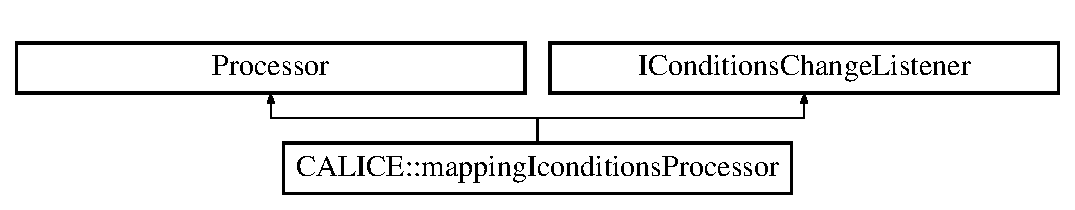
\includegraphics[height=2.000000cm]{classCALICE_1_1mappingIconditionsProcessor}
\end{center}
\end{figure}
\subsection*{Public Member Functions}
\begin{DoxyCompactItemize}
\item 
virtual Processor $\ast$ {\bf new\-Processor} ()
\item 
{\bf mapping\-Iconditions\-Processor} ()
\item 
virtual void {\bf init} ()
\item 
virtual void {\bf process\-Run\-Header} (L\-C\-Run\-Header $\ast$run)
\item 
virtual void {\bf process\-Event} (L\-C\-Event $\ast$evt)
\item 
virtual void {\bf end} ()
\end{DoxyCompactItemize}


\subsection{Detailed Description}
A processor which collects and provides the conditions data for the A\-H\-C\-A\-L modules.

\begin{DoxyRefDesc}{Todo}
\item[{\bf Todo}]
\begin{DoxyItemize}
\item get rid of hardcoded range numbers
\item get rid of hardcoded module index generation
\item use central mapping instead of re-\/implementing vrawadcprocessor
\end{DoxyItemize}\end{DoxyRefDesc}


\begin{DoxyAuthor}{Author}
B.\-Lutz 
\end{DoxyAuthor}
\begin{DoxyVersion}{Version}
2.\-0 
\end{DoxyVersion}
\begin{DoxyDate}{Date}
2010/06/15 
\end{DoxyDate}


\subsection{Constructor \& Destructor Documentation}
\index{C\-A\-L\-I\-C\-E\-::mapping\-Iconditions\-Processor@{C\-A\-L\-I\-C\-E\-::mapping\-Iconditions\-Processor}!mapping\-Iconditions\-Processor@{mapping\-Iconditions\-Processor}}
\index{mapping\-Iconditions\-Processor@{mapping\-Iconditions\-Processor}!CALICE::mappingIconditionsProcessor@{C\-A\-L\-I\-C\-E\-::mapping\-Iconditions\-Processor}}
\subsubsection[{mapping\-Iconditions\-Processor}]{\setlength{\rightskip}{0pt plus 5cm}C\-A\-L\-I\-C\-E\-::mapping\-Iconditions\-Processor\-::mapping\-Iconditions\-Processor (
\begin{DoxyParamCaption}
{}
\end{DoxyParamCaption}
)}\label{classCALICE_1_1mappingIconditionsProcessor_a9b19acde98a5704975cc9cdf0844ca01}
Default constructor 

Referenced by new\-Processor().



\subsection{Member Function Documentation}
\index{C\-A\-L\-I\-C\-E\-::mapping\-Iconditions\-Processor@{C\-A\-L\-I\-C\-E\-::mapping\-Iconditions\-Processor}!end@{end}}
\index{end@{end}!CALICE::mappingIconditionsProcessor@{C\-A\-L\-I\-C\-E\-::mapping\-Iconditions\-Processor}}
\subsubsection[{end}]{\setlength{\rightskip}{0pt plus 5cm}void C\-A\-L\-I\-C\-E\-::mapping\-Iconditions\-Processor\-::end (
\begin{DoxyParamCaption}
{}
\end{DoxyParamCaption}
)\hspace{0.3cm}{\ttfamily [virtual]}}\label{classCALICE_1_1mappingIconditionsProcessor_a7d36c4a2371a44c59119f7253a01e50a}
End of all events \index{C\-A\-L\-I\-C\-E\-::mapping\-Iconditions\-Processor@{C\-A\-L\-I\-C\-E\-::mapping\-Iconditions\-Processor}!init@{init}}
\index{init@{init}!CALICE::mappingIconditionsProcessor@{C\-A\-L\-I\-C\-E\-::mapping\-Iconditions\-Processor}}
\subsubsection[{init}]{\setlength{\rightskip}{0pt plus 5cm}void C\-A\-L\-I\-C\-E\-::mapping\-Iconditions\-Processor\-::init (
\begin{DoxyParamCaption}
{}
\end{DoxyParamCaption}
)\hspace{0.3cm}{\ttfamily [virtual]}}\label{classCALICE_1_1mappingIconditionsProcessor_a06daeeb584e240e5eb310ef432a450bc}
Initialize useful variables \index{C\-A\-L\-I\-C\-E\-::mapping\-Iconditions\-Processor@{C\-A\-L\-I\-C\-E\-::mapping\-Iconditions\-Processor}!new\-Processor@{new\-Processor}}
\index{new\-Processor@{new\-Processor}!CALICE::mappingIconditionsProcessor@{C\-A\-L\-I\-C\-E\-::mapping\-Iconditions\-Processor}}
\subsubsection[{new\-Processor}]{\setlength{\rightskip}{0pt plus 5cm}virtual Processor$\ast$ C\-A\-L\-I\-C\-E\-::mapping\-Iconditions\-Processor\-::new\-Processor (
\begin{DoxyParamCaption}
{}
\end{DoxyParamCaption}
)\hspace{0.3cm}{\ttfamily [inline]}, {\ttfamily [virtual]}}\label{classCALICE_1_1mappingIconditionsProcessor_a051c1a68f2fcf33bde820c9c190ed6d8}
Create a new instance of this processor 

References mapping\-Iconditions\-Processor().

\index{C\-A\-L\-I\-C\-E\-::mapping\-Iconditions\-Processor@{C\-A\-L\-I\-C\-E\-::mapping\-Iconditions\-Processor}!process\-Event@{process\-Event}}
\index{process\-Event@{process\-Event}!CALICE::mappingIconditionsProcessor@{C\-A\-L\-I\-C\-E\-::mapping\-Iconditions\-Processor}}
\subsubsection[{process\-Event}]{\setlength{\rightskip}{0pt plus 5cm}void C\-A\-L\-I\-C\-E\-::mapping\-Iconditions\-Processor\-::process\-Event (
\begin{DoxyParamCaption}
\item[{L\-C\-Event $\ast$}]{evt}
\end{DoxyParamCaption}
)\hspace{0.3cm}{\ttfamily [virtual]}}\label{classCALICE_1_1mappingIconditionsProcessor_a561ea75165004efdf734fcb251805c6d}
Process the event 
\begin{DoxyParams}{Parameters}
{\em evt} & the event to be processed \\
\hline
\end{DoxyParams}
\index{C\-A\-L\-I\-C\-E\-::mapping\-Iconditions\-Processor@{C\-A\-L\-I\-C\-E\-::mapping\-Iconditions\-Processor}!process\-Run\-Header@{process\-Run\-Header}}
\index{process\-Run\-Header@{process\-Run\-Header}!CALICE::mappingIconditionsProcessor@{C\-A\-L\-I\-C\-E\-::mapping\-Iconditions\-Processor}}
\subsubsection[{process\-Run\-Header}]{\setlength{\rightskip}{0pt plus 5cm}void C\-A\-L\-I\-C\-E\-::mapping\-Iconditions\-Processor\-::process\-Run\-Header (
\begin{DoxyParamCaption}
\item[{L\-C\-Run\-Header $\ast$}]{run}
\end{DoxyParamCaption}
)\hspace{0.3cm}{\ttfamily [virtual]}}\label{classCALICE_1_1mappingIconditionsProcessor_a8bd9ab85e8d6fdd50eeba5661d12358f}
Process the run header 
\begin{DoxyParams}{Parameters}
{\em run} & the run header to be processed \\
\hline
\end{DoxyParams}


The documentation for this class was generated from the following files\-:\begin{DoxyCompactItemize}
\item 
/nfs/dust/ilc/user/marquezh/\-Calice\-Soft\-\_\-w\-\_\-\-I\-L\-C\-Soft\-\_\-v02-\/03-\/02/calice\-\_\-analysis/addon\-Procs/include/mapping\-Iconditions\-Processor.\-hh\item 
/nfs/dust/ilc/user/marquezh/\-Calice\-Soft\-\_\-w\-\_\-\-I\-L\-C\-Soft\-\_\-v02-\/03-\/02/calice\-\_\-analysis/addon\-Procs/src/mapping\-Iconditions\-Processor.\-cc\end{DoxyCompactItemize}

\section{C\-A\-L\-I\-C\-E\-:\-:M\-C\-\_\-\-Truth\-\_\-info Class Reference}
\label{classCALICE_1_1MC__Truth__info}\index{C\-A\-L\-I\-C\-E\-::\-M\-C\-\_\-\-Truth\-\_\-info@{C\-A\-L\-I\-C\-E\-::\-M\-C\-\_\-\-Truth\-\_\-info}}
Inheritance diagram for C\-A\-L\-I\-C\-E\-:\-:M\-C\-\_\-\-Truth\-\_\-info\-:\begin{figure}[H]
\begin{center}
\leavevmode
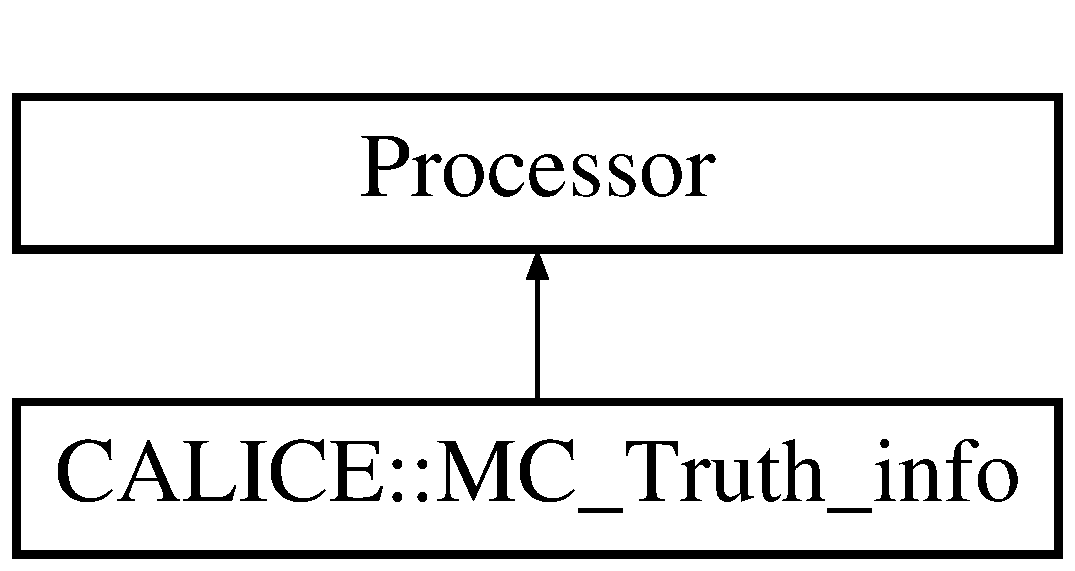
\includegraphics[height=2.000000cm]{classCALICE_1_1MC__Truth__info}
\end{center}
\end{figure}
\subsection*{Public Member Functions}
\begin{DoxyCompactItemize}
\item 
virtual Processor $\ast$ {\bfseries new\-Processor} ()\label{classCALICE_1_1MC__Truth__info_a9557dad836bc12f708b37690328adb54}

\item 
{\bf M\-C\-\_\-\-Truth\-\_\-info} ()
\item 
{\bf $\sim$\-M\-C\-\_\-\-Truth\-\_\-info} ()
\item 
virtual void {\bf init} ()
\item 
virtual void {\bf process\-Run\-Header} (L\-C\-Event $\ast$evt)
\item 
virtual void {\bf process\-Event} (L\-C\-Event $\ast$evt)
\item 
virtual void {\bf check} (L\-C\-Event $\ast$evt)
\item 
virtual void {\bf end} ()
\item 
void {\bfseries print\-Parameters} ()\label{classCALICE_1_1MC__Truth__info_aaa77c7af7ba04cd1ee023aba266592c6}

\end{DoxyCompactItemize}
\subsection*{Protected Attributes}
\begin{DoxyCompactItemize}
\item 
int {\bfseries \-\_\-n\-Evt}\label{classCALICE_1_1MC__Truth__info_a4ea313554fb10bf1dfe2482ba0933a18}

\item 
int {\bfseries \-\_\-n\-Run}\label{classCALICE_1_1MC__Truth__info_aa06c2ed366aea6c67ac1bc6939b548e1}

\item 
string {\bfseries \-\_\-evt\-Var\-Col\-Name}\label{classCALICE_1_1MC__Truth__info_ae0213bb47575309e9492662f88b9ae10}

\item 
string {\bfseries \-\_\-hit\-In\-Col\-Name}\label{classCALICE_1_1MC__Truth__info_a220b14afa0d139ec7194c010feec75c2}

\item 
string {\bfseries \-\_\-in\-Hit\-Var\-Col\-Name}\label{classCALICE_1_1MC__Truth__info_ab8a72cce76fb546e9044c296a55a7c03}

\item 
string {\bfseries \-\_\-\-M\-C\-Particle\-Col\-Name}\label{classCALICE_1_1MC__Truth__info_a888972e1205a9210eb9679248b3a6434}

\item 
string {\bfseries \-\_\-\-Simhit\-In\-Col\-Name}\label{classCALICE_1_1MC__Truth__info_ac4695b11df5d122bfc4a884e00b64366}

\item 
string {\bfseries \-\_\-calohit\-M\-C\-Truth\-Link}\label{classCALICE_1_1MC__Truth__info_a1a83f8dc2c3127c5114f071150eef241}

\item 
string {\bfseries \-\_\-hitvar\-Col\-Name}\label{classCALICE_1_1MC__Truth__info_a79cddb1c47620a2852046512139abe2c}

\item 
int {\bfseries P\-D\-G\-\_\-contribution}\label{classCALICE_1_1MC__Truth__info_acbfc836dfc2a3412f553867899f7a531}

\item 
int {\bfseries N\-M\-C\-\_\-contribution}\label{classCALICE_1_1MC__Truth__info_a804318bbc2f68e64f523ea9820e479b8}

\item 
string {\bfseries \-\_\-\-Root\-M\-C}\label{classCALICE_1_1MC__Truth__info_a5c9137b1c2c9bf7e6786dcbd80f75cbe}

\end{DoxyCompactItemize}


\subsection{Constructor \& Destructor Documentation}
\index{C\-A\-L\-I\-C\-E\-::\-M\-C\-\_\-\-Truth\-\_\-info@{C\-A\-L\-I\-C\-E\-::\-M\-C\-\_\-\-Truth\-\_\-info}!M\-C\-\_\-\-Truth\-\_\-info@{M\-C\-\_\-\-Truth\-\_\-info}}
\index{M\-C\-\_\-\-Truth\-\_\-info@{M\-C\-\_\-\-Truth\-\_\-info}!CALICE::MC_Truth_info@{C\-A\-L\-I\-C\-E\-::\-M\-C\-\_\-\-Truth\-\_\-info}}
\subsubsection[{M\-C\-\_\-\-Truth\-\_\-info}]{\setlength{\rightskip}{0pt plus 5cm}C\-A\-L\-I\-C\-E\-::\-M\-C\-\_\-\-Truth\-\_\-info\-::\-M\-C\-\_\-\-Truth\-\_\-info (
\begin{DoxyParamCaption}
{}
\end{DoxyParamCaption}
)}\label{classCALICE_1_1MC__Truth__info_a4fea2461a677a9c7e80859156edc790a}
Default constructor. \index{C\-A\-L\-I\-C\-E\-::\-M\-C\-\_\-\-Truth\-\_\-info@{C\-A\-L\-I\-C\-E\-::\-M\-C\-\_\-\-Truth\-\_\-info}!$\sim$\-M\-C\-\_\-\-Truth\-\_\-info@{$\sim$\-M\-C\-\_\-\-Truth\-\_\-info}}
\index{$\sim$\-M\-C\-\_\-\-Truth\-\_\-info@{$\sim$\-M\-C\-\_\-\-Truth\-\_\-info}!CALICE::MC_Truth_info@{C\-A\-L\-I\-C\-E\-::\-M\-C\-\_\-\-Truth\-\_\-info}}
\subsubsection[{$\sim$\-M\-C\-\_\-\-Truth\-\_\-info}]{\setlength{\rightskip}{0pt plus 5cm}C\-A\-L\-I\-C\-E\-::\-M\-C\-\_\-\-Truth\-\_\-info\-::$\sim$\-M\-C\-\_\-\-Truth\-\_\-info (
\begin{DoxyParamCaption}
{}
\end{DoxyParamCaption}
)\hspace{0.3cm}{\ttfamily [inline]}}\label{classCALICE_1_1MC__Truth__info_a82ea4e0cb59beff0aad1080d82ffe0e4}
Default destructor. 

\subsection{Member Function Documentation}
\index{C\-A\-L\-I\-C\-E\-::\-M\-C\-\_\-\-Truth\-\_\-info@{C\-A\-L\-I\-C\-E\-::\-M\-C\-\_\-\-Truth\-\_\-info}!check@{check}}
\index{check@{check}!CALICE::MC_Truth_info@{C\-A\-L\-I\-C\-E\-::\-M\-C\-\_\-\-Truth\-\_\-info}}
\subsubsection[{check}]{\setlength{\rightskip}{0pt plus 5cm}void C\-A\-L\-I\-C\-E\-::\-M\-C\-\_\-\-Truth\-\_\-info\-::check (
\begin{DoxyParamCaption}
\item[{L\-C\-Event $\ast$}]{evt}
\end{DoxyParamCaption}
)\hspace{0.3cm}{\ttfamily [virtual]}}\label{classCALICE_1_1MC__Truth__info_a3bbf13ce7c4566dbae859321944c301a}
Marlin \doxyref{check()}{p.}{classCALICE_1_1MC__Truth__info_a3bbf13ce7c4566dbae859321944c301a} function. \index{C\-A\-L\-I\-C\-E\-::\-M\-C\-\_\-\-Truth\-\_\-info@{C\-A\-L\-I\-C\-E\-::\-M\-C\-\_\-\-Truth\-\_\-info}!end@{end}}
\index{end@{end}!CALICE::MC_Truth_info@{C\-A\-L\-I\-C\-E\-::\-M\-C\-\_\-\-Truth\-\_\-info}}
\subsubsection[{end}]{\setlength{\rightskip}{0pt plus 5cm}void C\-A\-L\-I\-C\-E\-::\-M\-C\-\_\-\-Truth\-\_\-info\-::end (
\begin{DoxyParamCaption}
{}
\end{DoxyParamCaption}
)\hspace{0.3cm}{\ttfamily [virtual]}}\label{classCALICE_1_1MC__Truth__info_abc7036ee23408cf10013c0fc7686560b}
Marlin \doxyref{end()}{p.}{classCALICE_1_1MC__Truth__info_abc7036ee23408cf10013c0fc7686560b} function. \index{C\-A\-L\-I\-C\-E\-::\-M\-C\-\_\-\-Truth\-\_\-info@{C\-A\-L\-I\-C\-E\-::\-M\-C\-\_\-\-Truth\-\_\-info}!init@{init}}
\index{init@{init}!CALICE::MC_Truth_info@{C\-A\-L\-I\-C\-E\-::\-M\-C\-\_\-\-Truth\-\_\-info}}
\subsubsection[{init}]{\setlength{\rightskip}{0pt plus 5cm}void C\-A\-L\-I\-C\-E\-::\-M\-C\-\_\-\-Truth\-\_\-info\-::init (
\begin{DoxyParamCaption}
{}
\end{DoxyParamCaption}
)\hspace{0.3cm}{\ttfamily [virtual]}}\label{classCALICE_1_1MC__Truth__info_a84b4239852d2849e1574594d243fa1fa}
Marlin \doxyref{init()}{p.}{classCALICE_1_1MC__Truth__info_a84b4239852d2849e1574594d243fa1fa} function. \index{C\-A\-L\-I\-C\-E\-::\-M\-C\-\_\-\-Truth\-\_\-info@{C\-A\-L\-I\-C\-E\-::\-M\-C\-\_\-\-Truth\-\_\-info}!process\-Event@{process\-Event}}
\index{process\-Event@{process\-Event}!CALICE::MC_Truth_info@{C\-A\-L\-I\-C\-E\-::\-M\-C\-\_\-\-Truth\-\_\-info}}
\subsubsection[{process\-Event}]{\setlength{\rightskip}{0pt plus 5cm}void C\-A\-L\-I\-C\-E\-::\-M\-C\-\_\-\-Truth\-\_\-info\-::process\-Event (
\begin{DoxyParamCaption}
\item[{L\-C\-Event $\ast$}]{evt}
\end{DoxyParamCaption}
)\hspace{0.3cm}{\ttfamily [virtual]}}\label{classCALICE_1_1MC__Truth__info_a35db926a876c380b71cf8c98c3fce433}
Marlin \doxyref{process\-Event()}{p.}{classCALICE_1_1MC__Truth__info_a35db926a876c380b71cf8c98c3fce433} function. \index{C\-A\-L\-I\-C\-E\-::\-M\-C\-\_\-\-Truth\-\_\-info@{C\-A\-L\-I\-C\-E\-::\-M\-C\-\_\-\-Truth\-\_\-info}!process\-Run\-Header@{process\-Run\-Header}}
\index{process\-Run\-Header@{process\-Run\-Header}!CALICE::MC_Truth_info@{C\-A\-L\-I\-C\-E\-::\-M\-C\-\_\-\-Truth\-\_\-info}}
\subsubsection[{process\-Run\-Header}]{\setlength{\rightskip}{0pt plus 5cm}void C\-A\-L\-I\-C\-E\-::\-M\-C\-\_\-\-Truth\-\_\-info\-::process\-Run\-Header (
\begin{DoxyParamCaption}
\item[{L\-C\-Event $\ast$}]{evt}
\end{DoxyParamCaption}
)\hspace{0.3cm}{\ttfamily [virtual]}}\label{classCALICE_1_1MC__Truth__info_a344b770f5130dcdb235bb825f2c4b3e8}
Marlin \doxyref{process\-Run\-Header()}{p.}{classCALICE_1_1MC__Truth__info_a344b770f5130dcdb235bb825f2c4b3e8} function. 

The documentation for this class was generated from the following files\-:\begin{DoxyCompactItemize}
\item 
/nfs/dust/ilc/user/marquezh/\-Calice\-Soft\-\_\-w\-\_\-\-I\-L\-C\-Soft\-\_\-v02-\/03-\/02/calice\-\_\-analysis/addon\-Procs/include/M\-C\-\_\-\-Truth\-\_\-info.\-hh\item 
/nfs/dust/ilc/user/marquezh/\-Calice\-Soft\-\_\-w\-\_\-\-I\-L\-C\-Soft\-\_\-v02-\/03-\/02/calice\-\_\-analysis/addon\-Procs/src/M\-C\-\_\-\-Truth\-\_\-info.\-cc\end{DoxyCompactItemize}

\section{C\-A\-L\-I\-C\-E\-:\-:M\-C\-\_\-\-Truth\-\_\-\-Variables Class Reference}
\label{classCALICE_1_1MC__Truth__Variables}\index{C\-A\-L\-I\-C\-E\-::\-M\-C\-\_\-\-Truth\-\_\-\-Variables@{C\-A\-L\-I\-C\-E\-::\-M\-C\-\_\-\-Truth\-\_\-\-Variables}}
\subsection*{Public Member Functions}
\begin{DoxyCompactItemize}
\item 
{\bf M\-C\-\_\-\-Truth\-\_\-\-Variables} ()
\item 
{\bf $\sim$\-M\-C\-\_\-\-Truth\-\_\-\-Variables} ()
\item 
void {\bfseries Clear} ()\label{classCALICE_1_1MC__Truth__Variables_a907f4ef5d3a9ba7acfb75d4cae6316d8}

\end{DoxyCompactItemize}
\subsection*{Public Attributes}
\begin{DoxyCompactItemize}
\item 
vector$<$ int $>$ {\bfseries n\-Evt}\label{classCALICE_1_1MC__Truth__Variables_ade7a1e9eb44abf1d9b87a7c62bcc37ca}

\item 
vector$<$ double $>$ {\bfseries M\-C\-\_\-\-Cont\-\_\-\-Energy}\label{classCALICE_1_1MC__Truth__Variables_a0be460f76408acfb09ddd188ea8c31d0}

\end{DoxyCompactItemize}


\subsection{Constructor \& Destructor Documentation}
\index{C\-A\-L\-I\-C\-E\-::\-M\-C\-\_\-\-Truth\-\_\-\-Variables@{C\-A\-L\-I\-C\-E\-::\-M\-C\-\_\-\-Truth\-\_\-\-Variables}!M\-C\-\_\-\-Truth\-\_\-\-Variables@{M\-C\-\_\-\-Truth\-\_\-\-Variables}}
\index{M\-C\-\_\-\-Truth\-\_\-\-Variables@{M\-C\-\_\-\-Truth\-\_\-\-Variables}!CALICE::MC_Truth_Variables@{C\-A\-L\-I\-C\-E\-::\-M\-C\-\_\-\-Truth\-\_\-\-Variables}}
\subsubsection[{M\-C\-\_\-\-Truth\-\_\-\-Variables}]{\setlength{\rightskip}{0pt plus 5cm}C\-A\-L\-I\-C\-E\-::\-M\-C\-\_\-\-Truth\-\_\-\-Variables\-::\-M\-C\-\_\-\-Truth\-\_\-\-Variables (
\begin{DoxyParamCaption}
{}
\end{DoxyParamCaption}
)\hspace{0.3cm}{\ttfamily [inline]}}\label{classCALICE_1_1MC__Truth__Variables_a8d5a1c5c62669dab563faa4254f84eb3}
Constructor with member initialization \index{C\-A\-L\-I\-C\-E\-::\-M\-C\-\_\-\-Truth\-\_\-\-Variables@{C\-A\-L\-I\-C\-E\-::\-M\-C\-\_\-\-Truth\-\_\-\-Variables}!$\sim$\-M\-C\-\_\-\-Truth\-\_\-\-Variables@{$\sim$\-M\-C\-\_\-\-Truth\-\_\-\-Variables}}
\index{$\sim$\-M\-C\-\_\-\-Truth\-\_\-\-Variables@{$\sim$\-M\-C\-\_\-\-Truth\-\_\-\-Variables}!CALICE::MC_Truth_Variables@{C\-A\-L\-I\-C\-E\-::\-M\-C\-\_\-\-Truth\-\_\-\-Variables}}
\subsubsection[{$\sim$\-M\-C\-\_\-\-Truth\-\_\-\-Variables}]{\setlength{\rightskip}{0pt plus 5cm}C\-A\-L\-I\-C\-E\-::\-M\-C\-\_\-\-Truth\-\_\-\-Variables\-::$\sim$\-M\-C\-\_\-\-Truth\-\_\-\-Variables (
\begin{DoxyParamCaption}
{}
\end{DoxyParamCaption}
)\hspace{0.3cm}{\ttfamily [inline]}}\label{classCALICE_1_1MC__Truth__Variables_a00e9a62d94cd59ce5f8da31b4c2d212e}
Default destructor 

The documentation for this class was generated from the following file\-:\begin{DoxyCompactItemize}
\item 
/nfs/dust/ilc/user/marquezh/\-Calice\-Soft\-\_\-w\-\_\-\-I\-L\-C\-Soft\-\_\-v02-\/03-\/02/calice\-\_\-analysis/addon\-Procs/include/M\-C\-\_\-\-Truth\-\_\-info.\-hh\end{DoxyCompactItemize}

\section{Mc\-Frac\-Calc Class Reference}
\label{classMcFracCalc}\index{Mc\-Frac\-Calc@{Mc\-Frac\-Calc}}
Inheritance diagram for Mc\-Frac\-Calc\-:\begin{figure}[H]
\begin{center}
\leavevmode
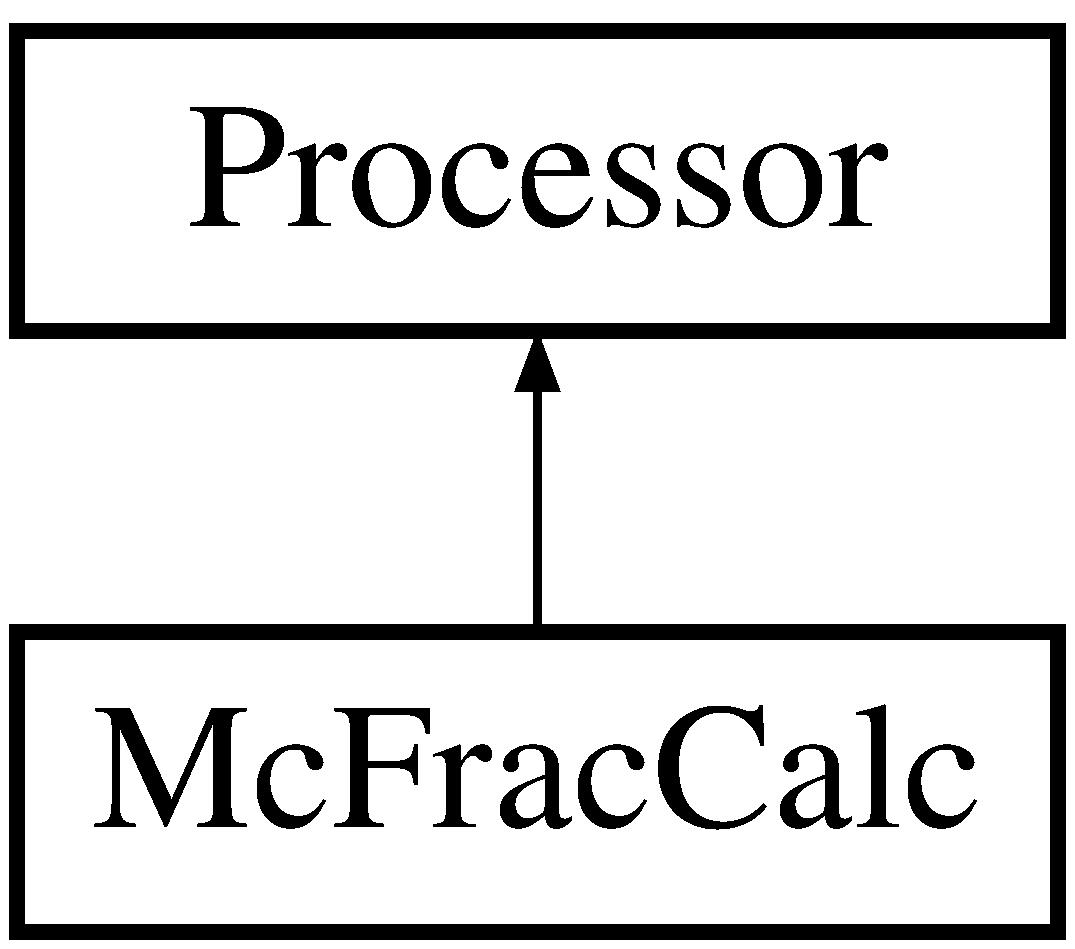
\includegraphics[height=2.000000cm]{classMcFracCalc}
\end{center}
\end{figure}
\subsection*{Public Member Functions}
\begin{DoxyCompactItemize}
\item 
{\bf Mc\-Frac\-Calc} $\ast$ {\bfseries new\-Processor} ()\label{classMcFracCalc_a70794f162a6cd9fa04740d30c1fc3f0b}

\item 
virtual void {\bfseries init} ()\label{classMcFracCalc_a038137333725929837afd82e5a333d03}

\item 
virtual void {\bfseries process\-Event} (lcio\-::\-L\-C\-Event $\ast$)\label{classMcFracCalc_a6f8ee7961e077134c9a9fed8c048bad4}

\item 
virtual void {\bfseries end} ()\label{classMcFracCalc_a0c614a1834dc43652c9f85fe54a7db38}

\item 
bool {\bfseries is\-Int} (std\-::string s)\label{classMcFracCalc_a2bedca9e1b3028460670a9787b8c6f6a}

\item 
int {\bfseries to\-Int} (const std\-::string s)\label{classMcFracCalc_ac0dcbd7322ef2860051f445ec58e8a71}

\end{DoxyCompactItemize}


The documentation for this class was generated from the following files\-:\begin{DoxyCompactItemize}
\item 
/nfs/dust/ilc/user/marquezh/\-Calice\-Soft\-\_\-w\-\_\-\-I\-L\-C\-Soft\-\_\-v02-\/03-\/02/calice\-\_\-analysis/addon\-Procs/include/Mc\-Frac\-Calc.\-hh\item 
/nfs/dust/ilc/user/marquezh/\-Calice\-Soft\-\_\-w\-\_\-\-I\-L\-C\-Soft\-\_\-v02-\/03-\/02/calice\-\_\-analysis/addon\-Procs/src/Mc\-Frac\-Calc.\-cc\end{DoxyCompactItemize}

\section{Mc\-Inverted\-Comp Class Reference}
\label{classMcInvertedComp}\index{Mc\-Inverted\-Comp@{Mc\-Inverted\-Comp}}
Inheritance diagram for Mc\-Inverted\-Comp\-:\begin{figure}[H]
\begin{center}
\leavevmode
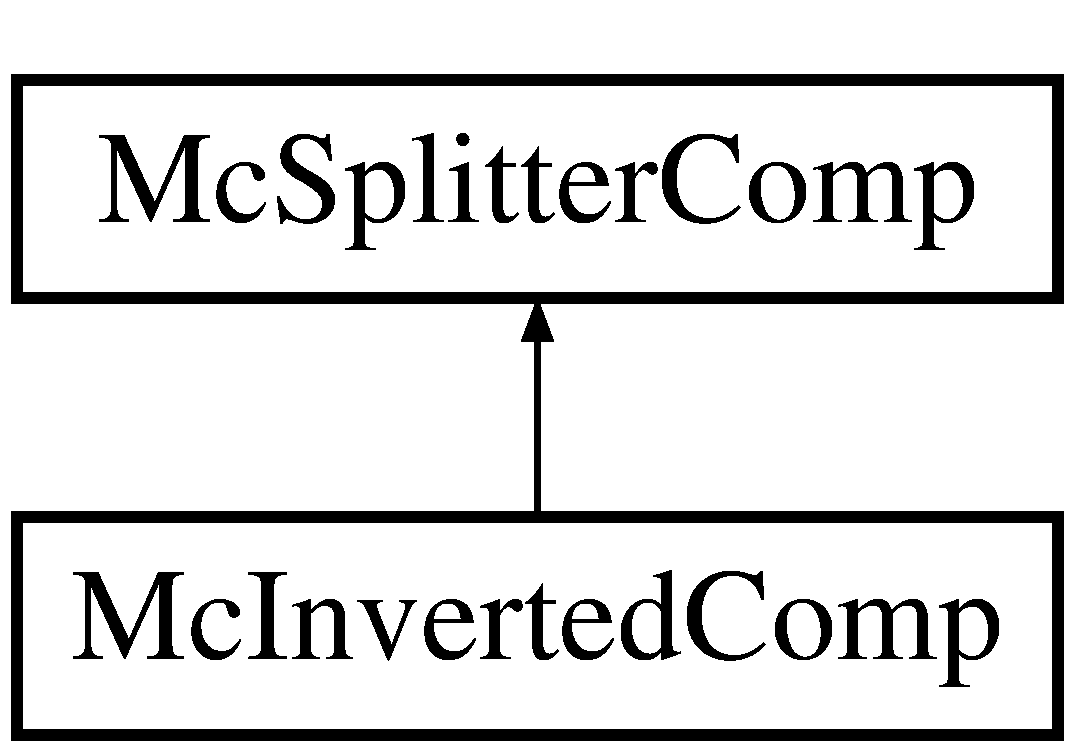
\includegraphics[height=2.000000cm]{classMcInvertedComp}
\end{center}
\end{figure}
\subsection*{Public Member Functions}
\begin{DoxyCompactItemize}
\item 
{\bfseries Mc\-Inverted\-Comp} (std\-::string name)\label{classMcInvertedComp_a0b9b203d745f4372de21fe11dcaac17e}

\item 
virtual bool {\bfseries matches} (const int pdg)\label{classMcInvertedComp_a83ce362b8040f1c685be622d7f0d2378}

\end{DoxyCompactItemize}


The documentation for this class was generated from the following files\-:\begin{DoxyCompactItemize}
\item 
/nfs/dust/ilc/user/marquezh/\-Calice\-Soft\-\_\-w\-\_\-\-I\-L\-C\-Soft\-\_\-v02-\/03-\/02/calice\-\_\-analysis/addon\-Procs/include/Mc\-Inverted\-Comp.\-hh\item 
/nfs/dust/ilc/user/marquezh/\-Calice\-Soft\-\_\-w\-\_\-\-I\-L\-C\-Soft\-\_\-v02-\/03-\/02/calice\-\_\-analysis/addon\-Procs/src/Mc\-Inverted\-Comp.\-cc\end{DoxyCompactItemize}

\section{Mc\-Splitter Class Reference}
\label{classMcSplitter}\index{Mc\-Splitter@{Mc\-Splitter}}
Inheritance diagram for Mc\-Splitter\-:\begin{figure}[H]
\begin{center}
\leavevmode
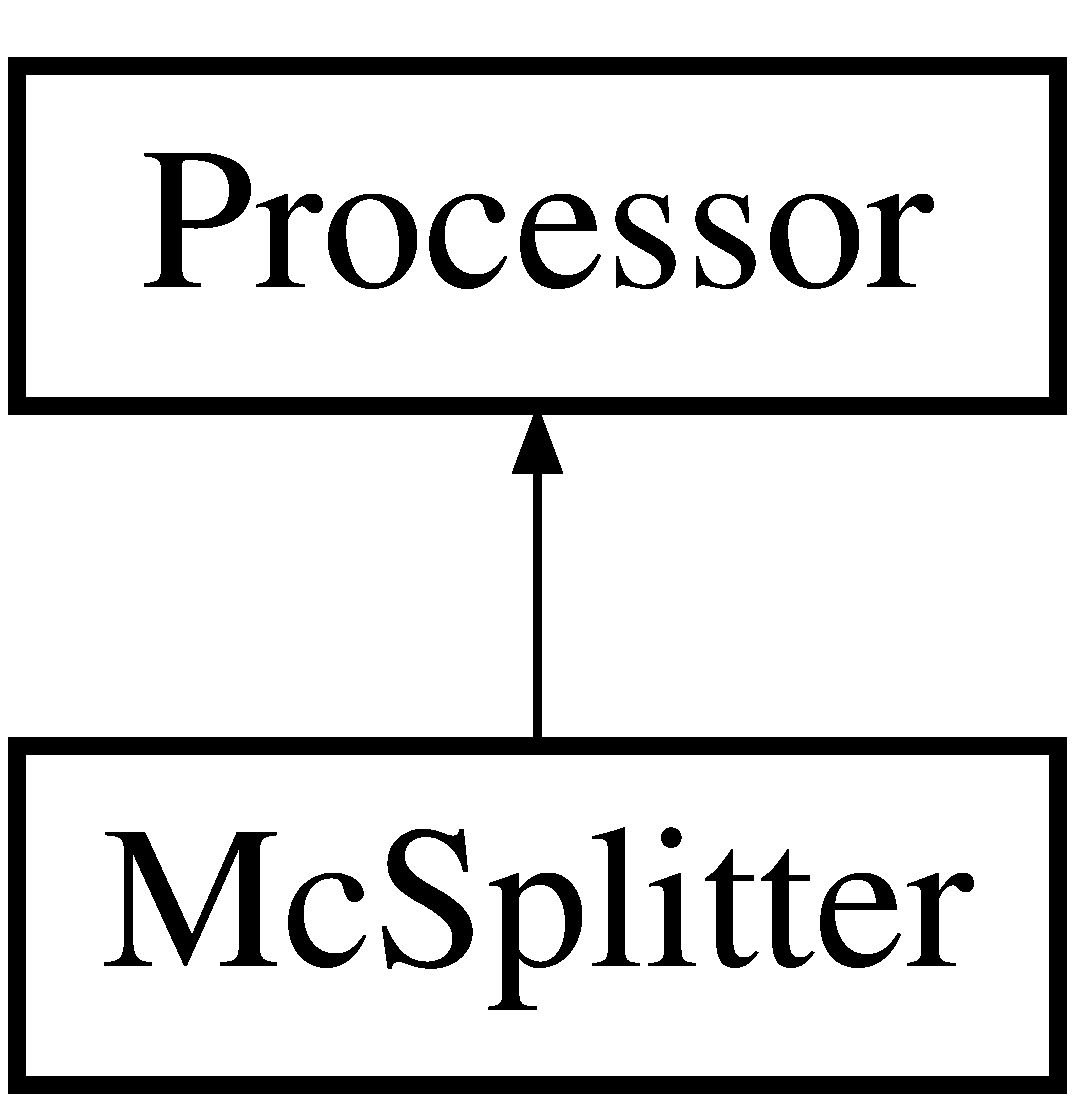
\includegraphics[height=2.000000cm]{classMcSplitter}
\end{center}
\end{figure}
\subsection*{Public Member Functions}
\begin{DoxyCompactItemize}
\item 
{\bf Mc\-Splitter} $\ast$ {\bfseries new\-Processor} ()\label{classMcSplitter_a712b72cabe110e8069c97895dcf73706}

\item 
virtual void {\bfseries init} ()\label{classMcSplitter_af9b90148faf589c6fb7e6a1c718d03f2}

\item 
virtual void {\bfseries process\-Event} (lcio\-::\-L\-C\-Event $\ast$)\label{classMcSplitter_a139fcffe97218a69776de8cb119222ac}

\item 
virtual void {\bfseries end} ()\label{classMcSplitter_a0f97174737126b2daeeab00626b6441f}

\item 
bool {\bfseries is\-Int} (std\-::string s)\label{classMcSplitter_af733254b12fe00cc43dc066b4abf3885}

\item 
int {\bfseries to\-Int} (const std\-::string s)\label{classMcSplitter_af432df32a9c3064ee0e3af878b55d301}

\end{DoxyCompactItemize}


The documentation for this class was generated from the following files\-:\begin{DoxyCompactItemize}
\item 
/nfs/dust/ilc/user/marquezh/\-Calice\-Soft\-\_\-w\-\_\-\-I\-L\-C\-Soft\-\_\-v02-\/03-\/02/calice\-\_\-analysis/addon\-Procs/include/Mc\-Splitter.\-hh\item 
/nfs/dust/ilc/user/marquezh/\-Calice\-Soft\-\_\-w\-\_\-\-I\-L\-C\-Soft\-\_\-v02-\/03-\/02/calice\-\_\-analysis/addon\-Procs/src/Mc\-Splitter.\-cc\end{DoxyCompactItemize}

\section{Mc\-Splitter\-Comp Class Reference}
\label{classMcSplitterComp}\index{Mc\-Splitter\-Comp@{Mc\-Splitter\-Comp}}
Inheritance diagram for Mc\-Splitter\-Comp\-:\begin{figure}[H]
\begin{center}
\leavevmode
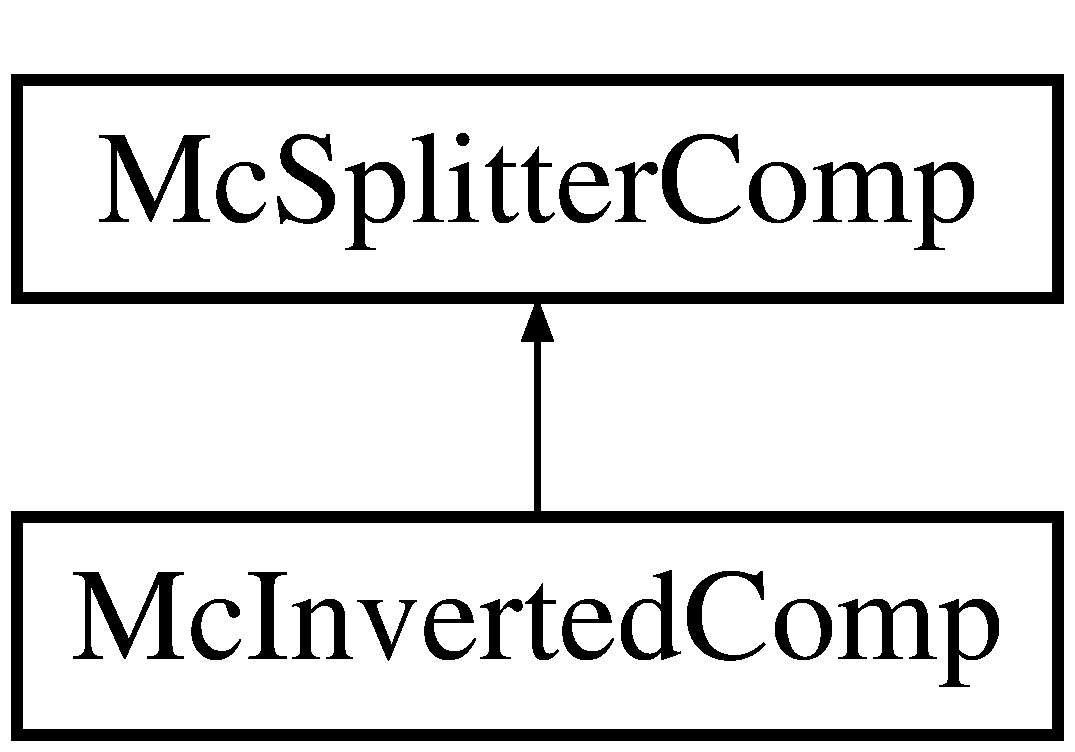
\includegraphics[height=2.000000cm]{classMcSplitterComp}
\end{center}
\end{figure}
\subsection*{Public Member Functions}
\begin{DoxyCompactItemize}
\item 
{\bfseries Mc\-Splitter\-Comp} (const std\-::string name)\label{classMcSplitterComp_a5e3be4628166a5c07964a3b59ed6316b}

\item 
virtual std\-::string {\bfseries name} ()\label{classMcSplitterComp_a2a0ac3a730c7befd38ab667537932fd5}

\item 
virtual void {\bfseries add\-P\-D\-G} (const int pdg)\label{classMcSplitterComp_a7ae84183e5de08aa08826a1570ef062c}

\item 
virtual bool {\bfseries matches} (const int pdg)\label{classMcSplitterComp_a4b5d625f2ad7b7f740203ab33f065ae6}

\item 
virtual void {\bfseries add\-Energy} (const float energy)\label{classMcSplitterComp_a6a0ce42a9b668115f4df8529ebbfd922}

\item 
virtual void {\bfseries reset\-Energy} ()\label{classMcSplitterComp_a1d74571f28b38b2b7a585cfe43986bc9}

\item 
virtual float {\bfseries energy} ()\label{classMcSplitterComp_a928ad84818b0b16fb948204761cae809}

\item 
virtual void {\bfseries copy\-Stuff\-From} (E\-V\-E\-N\-T\-::\-Sim\-Calorimeter\-Hit $\ast$hit)\label{classMcSplitterComp_a82f114e76b85200ce7ded5914c3c2607}

\item 
virtual \\*
I\-M\-P\-L\-::\-Sim\-Calorimeter\-Hit\-Impl $\ast$ {\bfseries create\-Sim\-Calorimeter\-Hit\-Impl} ()\label{classMcSplitterComp_ad133f4bf8456faeb30e173e6c24a6b2b}

\end{DoxyCompactItemize}


The documentation for this class was generated from the following files\-:\begin{DoxyCompactItemize}
\item 
/nfs/dust/ilc/user/marquezh/\-Calice\-Soft\-\_\-w\-\_\-\-I\-L\-C\-Soft\-\_\-v02-\/03-\/02/calice\-\_\-analysis/addon\-Procs/include/Mc\-Splitter\-Comp.\-hh\item 
/nfs/dust/ilc/user/marquezh/\-Calice\-Soft\-\_\-w\-\_\-\-I\-L\-C\-Soft\-\_\-v02-\/03-\/02/calice\-\_\-analysis/addon\-Procs/src/Mc\-Splitter\-Comp.\-cc\end{DoxyCompactItemize}

\section{C\-A\-L\-I\-C\-E\-:\-:Merge\-Processor Class Reference}
\label{classCALICE_1_1MergeProcessor}\index{C\-A\-L\-I\-C\-E\-::\-Merge\-Processor@{C\-A\-L\-I\-C\-E\-::\-Merge\-Processor}}
Inheritance diagram for C\-A\-L\-I\-C\-E\-:\-:Merge\-Processor\-:\begin{figure}[H]
\begin{center}
\leavevmode
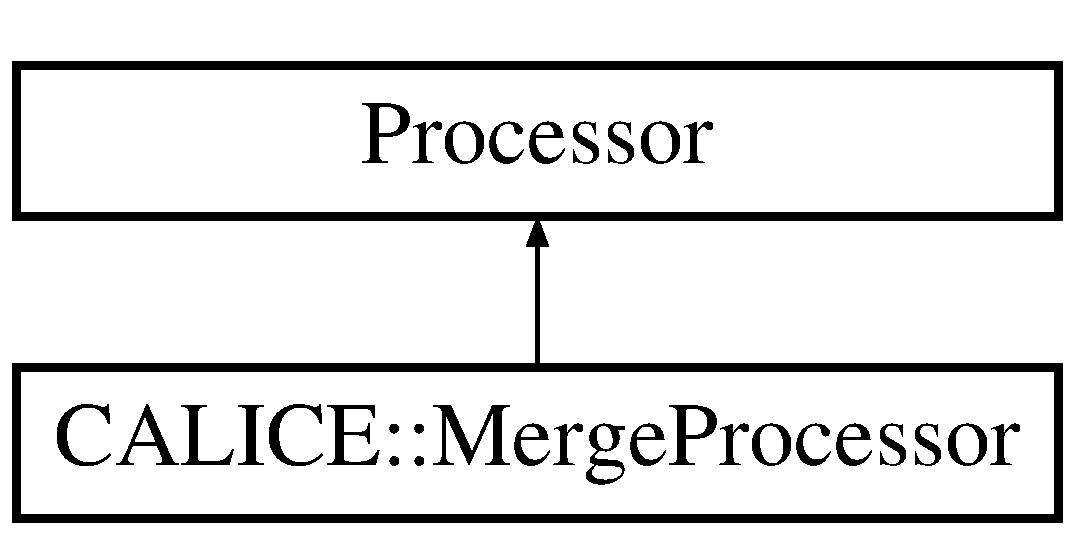
\includegraphics[height=2.000000cm]{classCALICE_1_1MergeProcessor}
\end{center}
\end{figure}
\subsection*{Public Member Functions}
\begin{DoxyCompactItemize}
\item 
virtual Processor $\ast$ {\bfseries new\-Processor} ()\label{classCALICE_1_1MergeProcessor_a80588425ec0fc5d6c87eca2d5ef1f693}

\item 
virtual void {\bfseries init} ()\label{classCALICE_1_1MergeProcessor_a142cbdd317425b544d49c7daab3005b6}

\item 
virtual void {\bfseries process\-Run\-Header} (L\-C\-Run\-Header $\ast$run)\label{classCALICE_1_1MergeProcessor_ab35dbd0a58ed6d768e065f0919ce018f}

\item 
virtual void {\bfseries process\-Event} (L\-C\-Event $\ast$evt)\label{classCALICE_1_1MergeProcessor_ac52a52d3a922ce38868484703100d3b1}

\item 
virtual void {\bfseries check} (L\-C\-Event $\ast$evt)\label{classCALICE_1_1MergeProcessor_a7179f7f6f3cca70b3653b995eb8db37e}

\item 
virtual void {\bfseries end} ()\label{classCALICE_1_1MergeProcessor_ab76fdd20121a0d13ec7b634b17b17734}

\item 
virtual void {\bfseries print\-Parameters} ()\label{classCALICE_1_1MergeProcessor_a8320e519ba63d6f1f61f24cb0f64ea97}

\item 
void {\bfseries merge} (L\-C\-Collection $\ast$src1, L\-C\-Collection $\ast$src2, L\-C\-Collection\-Vec $\ast$dest)\label{classCALICE_1_1MergeProcessor_a5981b1d2303251571a0b18d4a9842c21}

\item 
E\-V\-E\-N\-T\-::\-L\-C\-Event $\ast$ {\bfseries read\-Next\-Event} (int event\-\_\-index)\label{classCALICE_1_1MergeProcessor_a781da33661648256a664cacb9db5fe1d}

\end{DoxyCompactItemize}


The documentation for this class was generated from the following files\-:\begin{DoxyCompactItemize}
\item 
/nfs/dust/ilc/user/marquezh/\-Calice\-Soft\-\_\-w\-\_\-\-I\-L\-C\-Soft\-\_\-v02-\/03-\/02/calice\-\_\-analysis/addon\-Procs/include/Merge\-Processor.\-h\item 
/nfs/dust/ilc/user/marquezh/\-Calice\-Soft\-\_\-w\-\_\-\-I\-L\-C\-Soft\-\_\-v02-\/03-\/02/calice\-\_\-analysis/addon\-Procs/src/Merge\-Processor.\-cc\end{DoxyCompactItemize}

\section{Mixture Class Reference}
\label{classMixture}\index{Mixture@{Mixture}}


{\ttfamily \#include $<$Mixture.\-hh$>$}

Inheritance diagram for Mixture\-:\begin{figure}[H]
\begin{center}
\leavevmode
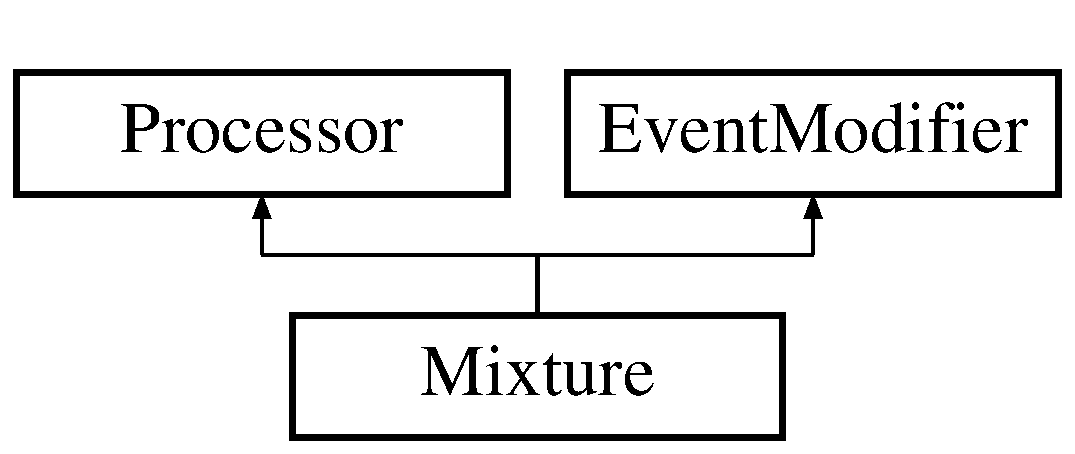
\includegraphics[height=2.000000cm]{classMixture}
\end{center}
\end{figure}
\subsection*{Public Member Functions}
\begin{DoxyCompactItemize}
\item 
virtual Processor $\ast$ {\bfseries new\-Processor} ()\label{classMixture_a974eea4854e24fca74828b6fb0d819d5}

\item 
virtual const std\-::string \& {\bfseries name} () const \label{classMixture_a69d184efcf89c019ef80b053a31ab674}

\item 
virtual void {\bfseries modify\-Event} (L\-C\-Event $\ast$evt)\label{classMixture_ae75b52d146c7099c2ebe9b5ce49f459b}

\item 
virtual void {\bfseries init} ()\label{classMixture_aa7c954d87460d3af08842e6d74e349a3}

\item 
virtual void {\bfseries process\-Run\-Header} (L\-C\-Run\-Header $\ast$run)\label{classMixture_a952a1875c684d2c13488efb0afeaa06a}

\item 
virtual void {\bfseries check} (L\-C\-Event $\ast$evt)\label{classMixture_ae08333282d6a417414ce2a1dc71bca15}

\item 
virtual void {\bfseries end} ()\label{classMixture_a3306b1afd0d8c8e0337feae3d6b66390}

\end{DoxyCompactItemize}
\subsection*{Protected Attributes}
\begin{DoxyCompactItemize}
\item 
String\-Vec {\bf \-\_\-input\-File\-Names}
\item 
int {\bfseries \-\_\-num\-Mixture}\label{classMixture_ae60aa285e3c3c7c8b1ee40fc3d25a999}

\item 
std\-::vector$<$ L\-C\-Reader $\ast$ $>$ {\bfseries \-\_\-lc\-Readers}\label{classMixture_a6716ae4c3996d3fa3fc236611b2d0a4a}

\item 
std\-::vector$<$ float $>$ {\bf \-\_\-\-X\-Y\-\_\-shifts}
\item 
int {\bfseries \-\_\-num\-Shifts}\label{classMixture_a2702eb808bc0b7ee05c9acbbe94bc1d2}

\item 
std\-::string {\bfseries \-\_\-\-E\-C\-A\-L\-Hits\-Col}\label{classMixture_a725049116e64f5aa4e9e9258c6c4b471}

\item 
std\-::string {\bfseries \-\_\-\-H\-C\-A\-L\-Hits\-Col}\label{classMixture_ad88306876cc621965682e03cb62cbb09}

\item 
std\-::string {\bfseries \-\_\-prop\-Col}\label{classMixture_a0d090f78a480f022f4f8162d20bbbd38}

\item 
float {\bfseries ampl} [200][200][100]\label{classMixture_ac74297cf6e6b0d69c0dbd2e1e6c69717}

\item 
float {\bfseries emip\-\_\-vis}\label{classMixture_aabebb58587585833b39487b83bd104a8}

\item 
float {\bfseries hmip\-\_\-vis}\label{classMixture_ac03d33567452f7414b98a6f3514f11be}

\item 
float {\bfseries ecal\-\_\-coeff1}\label{classMixture_ac74952885c910557ecf910feac27f927}

\item 
float {\bfseries ecal\-\_\-coeff2}\label{classMixture_acf97fa1e1fd6a61e0a3915d71be7ae35}

\item 
float {\bfseries ecal\-\_\-coeff3}\label{classMixture_a948d1c022842622b359dd26cb7275ecb}

\item 
float {\bfseries hcal\-\_\-coeff1}\label{classMixture_aade5aabafc94193e21197ef1e9022d9a}

\item 
float {\bfseries hcal\-\_\-coeff2}\label{classMixture_acb3c8ea43025ed4cf15a2ac41f30cef8}

\item 
float {\bfseries tcal\-\_\-coeff1}\label{classMixture_a0de3298a32af62efc1f81b41435c0521}

\item 
float {\bfseries tcal\-\_\-coeff2}\label{classMixture_a8cd33e93fc05fedfa123056715d3f201}

\item 
int {\bfseries last\-\_\-layer}\label{classMixture_ab19effdaeb9cc9e48cd2f69bc8d6d2cb}

\item 
float {\bfseries er\-\_\-inner}\label{classMixture_a4974a78d2ebdce70f9da0a8218eef291}

\item 
float {\bfseries er\-\_\-outer}\label{classMixture_ac321d3f65d7461619949a321bd77aa63}

\item 
float {\bfseries ez\-\_\-inner}\label{classMixture_ae24aebd80e43efce1d2212bb22b5f841}

\item 
float {\bfseries ez\-\_\-outer}\label{classMixture_a32a3674234fa205ce0e22c45a8dc1792}

\item 
float {\bfseries en\-\_\-sampl}\label{classMixture_aa180a7e0f57f0cf6dee5e4be64816f3a}

\item 
float {\bfseries esampling\-\_\-1}\label{classMixture_a28fcee8e2e04db5fa57c809586e390af}

\item 
float {\bfseries esampling\-\_\-2}\label{classMixture_ad5476769631a80e20d16fb379fa6130a}

\item 
float {\bfseries esampling\-\_\-3}\label{classMixture_a453e49e958b5881f5025cc61921671a5}

\item 
int {\bfseries emin\-\_\-lay}\label{classMixture_a5d362fb2cde4351916095bbc3c8dc9f5}

\item 
int {\bfseries emax\-\_\-lay}\label{classMixture_a6b3a9df3567aebda0aa8ca2f553e021e}

\item 
float {\bfseries eabsorber}\label{classMixture_af35bc54f80aa148e41bfe610d8d91bcb}

\item 
float {\bfseries ecell\-\_\-size}\label{classMixture_a4eb6bcf5e95363459526cc53ef894bce}

\item 
float {\bfseries hr\-\_\-inner}\label{classMixture_ae13328b3a2c043be7b57d11d376d062e}

\item 
float {\bfseries hr\-\_\-outer}\label{classMixture_a9dfdb824bd9bf9c1115bbe3f8e498f4d}

\item 
float {\bfseries hz\-\_\-inner}\label{classMixture_ab7c3c4d05d02acd2b1668e67453f89be}

\item 
float {\bfseries hz\-\_\-outer}\label{classMixture_a7fe392f5e3d7e8d1f2e1df764a224209}

\item 
float {\bfseries hn\-\_\-sampl}\label{classMixture_a2e8b19148b1e7fef5569d7cf489f7886}

\item 
float {\bfseries hsampling}\label{classMixture_a5c99ddcbb2edbe612ffe5cc2d6e9c1cb}

\item 
int {\bfseries hmin\-\_\-lay}\label{classMixture_a3afe6986acf26f835428c40bb340ee72}

\item 
int {\bfseries hmax\-\_\-lay}\label{classMixture_a89efdf94eaa4875ce02912d2dcead8c8}

\item 
float {\bfseries habsorber}\label{classMixture_a11cbb2d621914a350630360c4b1e5180}

\item 
float {\bfseries hcell\-\_\-size}\label{classMixture_a59546d9c7d344d3724a5f68e114f3746}

\item 
int {\bfseries \-\_\-n\-Run}\label{classMixture_a936e0cd135c37e348e81ec199ccbe9a5}

\item 
int {\bfseries \-\_\-n\-Evt}\label{classMixture_a34621d40b93176a49cb3e0cbe4d573ab}

\end{DoxyCompactItemize}


\subsection{Detailed Description}
\doxyref{Mixture}{p.}{classMixture} processor reads a few files with C\-A\-L\-I\-C\-E data selected events and joint them by suming-\/up all of them into one artificial event to use it in any reconstruction program.

\doxyref{Mixture}{p.}{classMixture} creates overlapped events from several especially prepared C\-A\-L\-I\-C\-E files

Processor creates two Calorimeter hit collections\-: Mixture\-E\-C\-A\-L and Mixture\-H\-C\-A\-L

List of input files should be restricted no more than 10 (0,1,2,3,4,5,6,7,8,9)

\doxyref{Mixture}{p.}{classMixture} processor copies all additional collections into E\-C\-A\-L0,E\-C\-A\-L1, ...,H\-C\-A\-L0,H\-C\-A\-L1, ..., T\-C\-A\-L0,T\-C\-A\-L1, ..., P\-T\-R\-K0,P\-T\-R\-K1, ... to have all of them at the final stage of Analysis.

First particle that is in main L\-C\-I\-O-\/file does not shifted; all additional particles that is in \-\_\-input\-File\-Names should have shifts of X and Y coordinates relatively to the first one. Vector \-\_\-\-X\-Y\-\_\-shifts

\begin{DoxyVerb}                          |                                             
                          |                                             
                          |                                             
                          |          First aditional particle in Mixture    
                          |           (X1,Y1)                           
                          |                                             
       Second additional  |                                             
                (X2,Y2)   |                                             
       particle           |                                             
                          |(0,0) X0,Y0 Zero particle in Mixture         
\end{DoxyVerb}
 -\/-\/-\/-\/-\/-\/-\/-\/-\/-\/-\/-\/-\/-\/-\/-\/-\/-\/-\/-\/-\/-\/-\/-\/-\/---$|$-\/-\/-\/-\/-\/-\/-\/-\/-\/-\/-\/-\/-\/-\/-\/-\/-\/-\/-\/-\/-\/-\/--- \begin{TabularC}{1}
\hline
\rowcolor{lightgray}{\bf }\\\cline{1-1}
\\\cline{1-1}
\end{TabularC}


\begin{DoxyAuthor}{Author}
V.\-L. Morgunov, I\-T\-E\-P 
\end{DoxyAuthor}
\begin{DoxyVersion}{Version}

\end{DoxyVersion}
\begin{DoxyParagraph}{Id\-:}
Mixture.\-h,v 1.\-0 2009/04/02 20\-:22\-:50 morgunov Exp 
\end{DoxyParagraph}



\begin{DoxyParams}{Parameters}
{\em Input\-File\-Names} & (String\-Vec) \\
\hline
\end{DoxyParams}


\subsection{Member Data Documentation}
\index{Mixture@{Mixture}!\-\_\-input\-File\-Names@{\-\_\-input\-File\-Names}}
\index{\-\_\-input\-File\-Names@{\-\_\-input\-File\-Names}!Mixture@{Mixture}}
\subsubsection[{\-\_\-input\-File\-Names}]{\setlength{\rightskip}{0pt plus 5cm}String\-Vec Mixture\-::\-\_\-input\-File\-Names\hspace{0.3cm}{\ttfamily [protected]}}\label{classMixture_ae40b0a91a75ffa96b02b40a22ba85e42}
Input file names. \index{Mixture@{Mixture}!\-\_\-\-X\-Y\-\_\-shifts@{\-\_\-\-X\-Y\-\_\-shifts}}
\index{\-\_\-\-X\-Y\-\_\-shifts@{\-\_\-\-X\-Y\-\_\-shifts}!Mixture@{Mixture}}
\subsubsection[{\-\_\-\-X\-Y\-\_\-shifts}]{\setlength{\rightskip}{0pt plus 5cm}std\-::vector$<$float$>$ Mixture\-::\-\_\-\-X\-Y\-\_\-shifts\hspace{0.3cm}{\ttfamily [protected]}}\label{classMixture_aa06ac7a8d75875a275decf16928d9b85}
Input coordinate shifts for that particles. 

The documentation for this class was generated from the following files\-:\begin{DoxyCompactItemize}
\item 
/nfs/dust/ilc/user/marquezh/\-Calice\-Soft\-\_\-w\-\_\-\-I\-L\-C\-Soft\-\_\-v02-\/03-\/02/calice\-\_\-analysis/addon\-Procs/include/Mixture.\-hh\item 
/nfs/dust/ilc/user/marquezh/\-Calice\-Soft\-\_\-w\-\_\-\-I\-L\-C\-Soft\-\_\-v02-\/03-\/02/calice\-\_\-analysis/addon\-Procs/src/Mixture.\-cc\end{DoxyCompactItemize}

\section{C\-A\-L\-I\-C\-E\-:\-:Multi\-Bit\-Generator Class Reference}
\label{classCALICE_1_1MultiBitGenerator}\index{C\-A\-L\-I\-C\-E\-::\-Multi\-Bit\-Generator@{C\-A\-L\-I\-C\-E\-::\-Multi\-Bit\-Generator}}


{\ttfamily \#include $<$Multi\-Bit\-Generator.\-hh$>$}

Inheritance diagram for C\-A\-L\-I\-C\-E\-:\-:Multi\-Bit\-Generator\-:\begin{figure}[H]
\begin{center}
\leavevmode
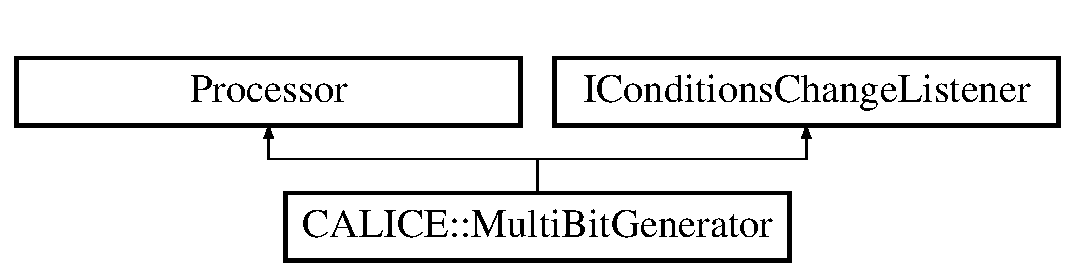
\includegraphics[height=2.000000cm]{classCALICE_1_1MultiBitGenerator}
\end{center}
\end{figure}
\subsection*{Public Member Functions}
\begin{DoxyCompactItemize}
\item 
Processor $\ast$ {\bfseries new\-Processor} ()\label{classCALICE_1_1MultiBitGenerator_a080c30da572966739180c5ad78b33726}

\item 
void {\bf init} ()
\item 
void {\bf process\-Run\-Header} (L\-C\-Run\-Header $\ast$run)
\item 
void {\bf process\-Event} (L\-C\-Event $\ast$evt)
\item 
void {\bfseries end} ()\label{classCALICE_1_1MultiBitGenerator_a9c66f8fc52d55b6185ee98d5d63b5b95}

\end{DoxyCompactItemize}
\subsection*{Protected Attributes}
\begin{DoxyCompactItemize}
\item 
std\-::string {\bfseries \-\_\-par\-Name\-Multi\-Amplitude}\label{classCALICE_1_1MultiBitGenerator_a54e51e094c859d5d8cad2a4d70415f0b}

\item 
std\-::string {\bfseries \-\_\-par\-Name\-Multi\-Bit}\label{classCALICE_1_1MultiBitGenerator_a2bb683f37ffefd42472f002425c1e184}

\item 
std\-::string {\bfseries \-\_\-threshold\-Col\-Name}\label{classCALICE_1_1MultiBitGenerator_a3d60b874142243c3161a22980c5add5f}

\item 
float {\bfseries \-\_\-set\-Purity}\label{classCALICE_1_1MultiBitGenerator_acdfc8dc40d3b785d401f534432b60e90}

\item 
float {\bfseries \-\_\-eff\-Purity}\label{classCALICE_1_1MultiBitGenerator_aa7af704d7fb005ee5374f6fe6852e27c}

\item 
float {\bfseries \-\_\-set\-Threshold}\label{classCALICE_1_1MultiBitGenerator_abc65d8c030a287e6e052fdfecea254f9}

\item 
float {\bfseries \-\_\-set\-Threshold\-Err}\label{classCALICE_1_1MultiBitGenerator_a9920211244785075a271343b7a122448}

\item 
bool {\bfseries \-\_\-fix\-Threshold}\label{classCALICE_1_1MultiBitGenerator_aa4724d6a3ae84e58da8c24cab192e2ac}

\end{DoxyCompactItemize}


\subsection{Detailed Description}
Processor which generates a trigger bit for particle multiplicity (P\-A\-R\-\_\-\-V\-E\-T\-O\-\_\-\-B\-I\-T) based on the multiplicity counter amplitude given by P\-A\-R\-\_\-\-M\-U\-L\-T\-I\-\_\-\-A\-M\-P\-L. The threshold values can be extracted from the database based on a chosen purity for the single-\/particle-\/sample (default) or be defined explicitly in the steering file (set \char`\"{}use\-Fixed\-Threshold\char`\"{} to \char`\"{}true\char`\"{}).

\begin{DoxyAuthor}{Author}
{\tt Benjamin.\-Lutz@desy.\-de} 

{\tt Nils.\-Feege@desy.\-de} 
\end{DoxyAuthor}
\begin{DoxyDate}{Date}
Mar 2010 
\end{DoxyDate}


\subsection{Member Function Documentation}
\index{C\-A\-L\-I\-C\-E\-::\-Multi\-Bit\-Generator@{C\-A\-L\-I\-C\-E\-::\-Multi\-Bit\-Generator}!init@{init}}
\index{init@{init}!CALICE::MultiBitGenerator@{C\-A\-L\-I\-C\-E\-::\-Multi\-Bit\-Generator}}
\subsubsection[{init}]{\setlength{\rightskip}{0pt plus 5cm}void C\-A\-L\-I\-C\-E\-::\-Multi\-Bit\-Generator\-::init (
\begin{DoxyParamCaption}
{}
\end{DoxyParamCaption}
)}\label{classCALICE_1_1MultiBitGenerator_ab3a76091024aee67a72bf47f197a76c6}
Called at the begin of the job before anything is read. Use to initialize the processor, e.\-g. book histograms. \index{C\-A\-L\-I\-C\-E\-::\-Multi\-Bit\-Generator@{C\-A\-L\-I\-C\-E\-::\-Multi\-Bit\-Generator}!process\-Event@{process\-Event}}
\index{process\-Event@{process\-Event}!CALICE::MultiBitGenerator@{C\-A\-L\-I\-C\-E\-::\-Multi\-Bit\-Generator}}
\subsubsection[{process\-Event}]{\setlength{\rightskip}{0pt plus 5cm}void C\-A\-L\-I\-C\-E\-::\-Multi\-Bit\-Generator\-::process\-Event (
\begin{DoxyParamCaption}
\item[{L\-C\-Event $\ast$}]{evt}
\end{DoxyParamCaption}
)}\label{classCALICE_1_1MultiBitGenerator_ab9b5cf63447e159929f34de39244ee32}
Called for every event -\/ the working horse. \index{C\-A\-L\-I\-C\-E\-::\-Multi\-Bit\-Generator@{C\-A\-L\-I\-C\-E\-::\-Multi\-Bit\-Generator}!process\-Run\-Header@{process\-Run\-Header}}
\index{process\-Run\-Header@{process\-Run\-Header}!CALICE::MultiBitGenerator@{C\-A\-L\-I\-C\-E\-::\-Multi\-Bit\-Generator}}
\subsubsection[{process\-Run\-Header}]{\setlength{\rightskip}{0pt plus 5cm}void C\-A\-L\-I\-C\-E\-::\-Multi\-Bit\-Generator\-::process\-Run\-Header (
\begin{DoxyParamCaption}
\item[{L\-C\-Run\-Header $\ast$}]{run}
\end{DoxyParamCaption}
)}\label{classCALICE_1_1MultiBitGenerator_a8e78905f379426472b533a53c86be977}
Called for every run, e.\-g. overwrite to initialize run dependent histograms. 

The documentation for this class was generated from the following files\-:\begin{DoxyCompactItemize}
\item 
/nfs/dust/ilc/user/marquezh/\-Calice\-Soft\-\_\-w\-\_\-\-I\-L\-C\-Soft\-\_\-v02-\/03-\/02/calice\-\_\-analysis/addon\-Procs/include/Multi\-Bit\-Generator.\-hh\item 
/nfs/dust/ilc/user/marquezh/\-Calice\-Soft\-\_\-w\-\_\-\-I\-L\-C\-Soft\-\_\-v02-\/03-\/02/calice\-\_\-analysis/addon\-Procs/src/Multi\-Bit\-Generator.\-cc\end{DoxyCompactItemize}

\section{my\-Cluster\-Ordering Class Reference}
\label{classmyClusterOrdering}\index{my\-Cluster\-Ordering@{my\-Cluster\-Ordering}}
\subsection*{Static Public Member Functions}
\begin{DoxyCompactItemize}
\item 
static bool {\bfseries compare\-Hit\-By\-Layer} (Calorimeter\-Hit $\ast$a\-Hit, Calorimeter\-Hit $\ast$b\-Hit)\label{classmyClusterOrdering_ac2904d36e505f78ed8c2f674228799eb}

\item 
static bool {\bfseries compare\-Vect\-By\-Size} (Cluster $\ast$cluster\-A, Cluster $\ast$cluster\-B)\label{classmyClusterOrdering_ad357e1d2c51a6cecd2f9419299b947dc}

\item 
static bool {\bfseries check\-X\-Y\-Adyacent\-Clusters} (Cluster $\ast$cluster\-A, Cluster $\ast$cluster\-B, float num\-Of\-Adyacent\-Cells)\label{classmyClusterOrdering_a6a73e211a8f1c576723b7e4357cd5f89}

\item 
static E\-V\-E\-N\-T\-::\-Cluster\-Vec {\bfseries merge\-Two\-Clusters} (E\-V\-E\-N\-T\-::\-Cluster $\ast$cluster\-A, E\-V\-E\-N\-T\-::\-Cluster $\ast$cluster\-B)\label{classmyClusterOrdering_a701c88add8e9a0e23f16dbe1bfbe9cf7}

\item 
static E\-V\-E\-N\-T\-::\-Cluster\-Vec {\bfseries remove\-Isolated\-Hits} (E\-V\-E\-N\-T\-::\-Cluster\-Vec sub\-Cluster)\label{classmyClusterOrdering_a6ca2324f45af090ad3ae381e712eda46}

\item 
static E\-V\-E\-N\-T\-::\-Cluster\-Vec {\bfseries obtain\-Sub\-Clusters} (E\-V\-E\-N\-T\-::\-Cluster $\ast$cluster\-A)\label{classmyClusterOrdering_a92fb99f4f6d0f278e57816aa800ec172}

\end{DoxyCompactItemize}


The documentation for this class was generated from the following file\-:\begin{DoxyCompactItemize}
\item 
/nfs/dust/ilc/user/marquezh/\-Calice\-Soft\-\_\-w\-\_\-\-I\-L\-C\-Soft\-\_\-v02-\/03-\/02/calice\-\_\-analysis/addon\-Procs/include/my\-Cluster\-Ordering.\-hh\end{DoxyCompactItemize}

\section{Point2\-D Class Reference}
\label{classPoint2D}\index{Point2\-D@{Point2\-D}}
\subsection*{Public Member Functions}
\begin{DoxyCompactItemize}
\item 
{\bfseries Point2\-D} (float ini)\label{classPoint2D_aa9bd636a920bba7115ac65e18ce2b137}

\end{DoxyCompactItemize}
\subsection*{Public Attributes}
\begin{DoxyCompactItemize}
\item 
float {\bfseries x}\label{classPoint2D_a2a5ef0ad00bc9e912a9aefcedf004cc4}

\item 
float {\bfseries y}\label{classPoint2D_a989485fd2d8026ceec5d57e8c7e629ab}

\end{DoxyCompactItemize}


The documentation for this class was generated from the following file\-:\begin{DoxyCompactItemize}
\item 
/nfs/dust/ilc/user/marquezh/\-Calice\-Soft\-\_\-w\-\_\-\-I\-L\-C\-Soft\-\_\-v02-\/03-\/02/calice\-\_\-analysis/addon\-Procs/include/Find\-Start\-And\-Primary\-Track.\-h\end{DoxyCompactItemize}

\section{Primary\-Track\-Finder Class Reference}
\label{classPrimaryTrackFinder}\index{Primary\-Track\-Finder@{Primary\-Track\-Finder}}


Marlin processor that finds shower start and primary track.  




{\ttfamily \#include $<$Primary\-Track\-Finder.\-hh$>$}

Inheritance diagram for Primary\-Track\-Finder\-:\begin{figure}[H]
\begin{center}
\leavevmode
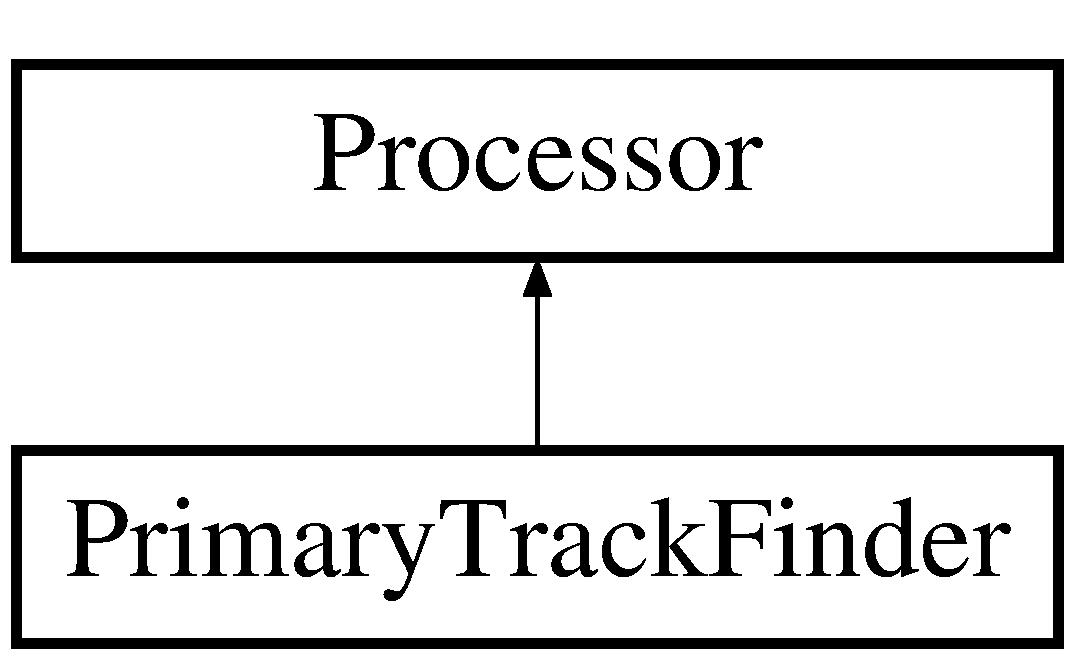
\includegraphics[height=2.000000cm]{classPrimaryTrackFinder}
\end{center}
\end{figure}
\subsection*{Public Member Functions}
\begin{DoxyCompactItemize}
\item 
{\bf Primary\-Track\-Finder} ()
\item 
virtual {\bf $\sim$\-Primary\-Track\-Finder} ()
\item 
{\bf Primary\-Track\-Finder} $\ast$ {\bfseries new\-Processor} ()\label{classPrimaryTrackFinder_a5138e4436f12055e84179818ec2ac9e8}

\item 
virtual void {\bf init} ()
\item 
virtual void {\bf process\-Run\-Header} (L\-C\-Run\-Header $\ast$)
\item 
virtual void {\bf process\-Event} (lcio\-::\-L\-C\-Event $\ast$)
\item 
virtual void {\bf end} ()
\item 
float {\bf dist\-X\-Y} ({\bf C\-Hit} $\ast$, {\bf C\-Hit} $\ast$)
\item 
unsigned {\bf get\-Starting\-Layer} ({\bf C\-Layer} $\ast$)
\item 
bool {\bf Find\-Track} (unsigned, {\bf C\-Layer} $\ast$)
\item 
bool {\bf is\-Muon} (float, float)
\end{DoxyCompactItemize}


\subsection{Detailed Description}
Marlin processor that finds shower start and primary track. 

In this processor Calorimeter\-Hit collections for E\-C\-A\-L and H\-C\-A\-L are used to find shower starting layer and hits belonging to ingoing track, these hits are then put into output collection of class Calorimeter\-Hit. In track output collection the following class members are set\-: Type -\/ hit layer number, Position -\/ X\-Y\-Z hit coordinates, Energy -\/ deposited energy in M\-I\-Ps. For shower starting layer, L\-C\-Generic\-Object collection has two integer members\-: calorimeter type (0 -\/ E\-C\-A\-L, 1 -\/ first 30 H\-C\-A\-L layers, 2 -\/ last coarse part of H\-C\-A\-L) shower starting layer number (in each calorimeter) and two float members\-: weighted average of x coordinate of track hits weighted average of y coordinate of track hits

\begin{DoxyVersion}{Version}
4.\-01 
\end{DoxyVersion}
\begin{DoxyAuthor}{Author}
M.\-V. Chadeeva 
\end{DoxyAuthor}
\begin{DoxyDate}{Date}
November 2010 
\end{DoxyDate}


\subsection{Constructor \& Destructor Documentation}
\index{Primary\-Track\-Finder@{Primary\-Track\-Finder}!Primary\-Track\-Finder@{Primary\-Track\-Finder}}
\index{Primary\-Track\-Finder@{Primary\-Track\-Finder}!PrimaryTrackFinder@{Primary\-Track\-Finder}}
\subsubsection[{Primary\-Track\-Finder}]{\setlength{\rightskip}{0pt plus 5cm}Primary\-Track\-Finder\-::\-Primary\-Track\-Finder (
\begin{DoxyParamCaption}
{}
\end{DoxyParamCaption}
)}\label{classPrimaryTrackFinder_ad80886cf9c522adf66e28e7556d33027}
Default constructor \index{Primary\-Track\-Finder@{Primary\-Track\-Finder}!$\sim$\-Primary\-Track\-Finder@{$\sim$\-Primary\-Track\-Finder}}
\index{$\sim$\-Primary\-Track\-Finder@{$\sim$\-Primary\-Track\-Finder}!PrimaryTrackFinder@{Primary\-Track\-Finder}}
\subsubsection[{$\sim$\-Primary\-Track\-Finder}]{\setlength{\rightskip}{0pt plus 5cm}Primary\-Track\-Finder\-::$\sim$\-Primary\-Track\-Finder (
\begin{DoxyParamCaption}
{}
\end{DoxyParamCaption}
)\hspace{0.3cm}{\ttfamily [virtual]}}\label{classPrimaryTrackFinder_afbf250d7baa1b884f2b07beda7e3e94f}
Default destructor 

\subsection{Member Function Documentation}
\index{Primary\-Track\-Finder@{Primary\-Track\-Finder}!dist\-X\-Y@{dist\-X\-Y}}
\index{dist\-X\-Y@{dist\-X\-Y}!PrimaryTrackFinder@{Primary\-Track\-Finder}}
\subsubsection[{dist\-X\-Y}]{\setlength{\rightskip}{0pt plus 5cm}float Primary\-Track\-Finder\-::dist\-X\-Y (
\begin{DoxyParamCaption}
\item[{{\bf C\-Hit} $\ast$}]{h1, }
\item[{{\bf C\-Hit} $\ast$}]{h2}
\end{DoxyParamCaption}
)}\label{classPrimaryTrackFinder_ac53641accf71821b0cf3361c835b1db9}
Calculates and returns distance between two hits in X\-Y-\/plane 

References C\-A\-L\-I\-C\-E\-::\-C\-Hit\-::x, and C\-A\-L\-I\-C\-E\-::\-C\-Hit\-::y.



Referenced by Find\-Track().

\index{Primary\-Track\-Finder@{Primary\-Track\-Finder}!end@{end}}
\index{end@{end}!PrimaryTrackFinder@{Primary\-Track\-Finder}}
\subsubsection[{end}]{\setlength{\rightskip}{0pt plus 5cm}void Primary\-Track\-Finder\-::end (
\begin{DoxyParamCaption}
{}
\end{DoxyParamCaption}
)\hspace{0.3cm}{\ttfamily [virtual]}}\label{classPrimaryTrackFinder_acd180f6ae6a0925be6cbdb06524c300c}
Function to close root-\/file and print some statistic results \index{Primary\-Track\-Finder@{Primary\-Track\-Finder}!Find\-Track@{Find\-Track}}
\index{Find\-Track@{Find\-Track}!PrimaryTrackFinder@{Primary\-Track\-Finder}}
\subsubsection[{Find\-Track}]{\setlength{\rightskip}{0pt plus 5cm}bool Primary\-Track\-Finder\-::\-Find\-Track (
\begin{DoxyParamCaption}
\item[{unsigned}]{start, }
\item[{{\bf C\-Layer} $\ast$}]{lr}
\end{DoxyParamCaption}
)}\label{classPrimaryTrackFinder_a22924bae502da65b35257062f6230957}
Finds hits belonging to primary track taking in account the earlier found shower starting layer. The \char`\"{}nearest neighbour\char`\"{} criteria is used. Maximum distance parameters are defined taking in account the cell size. First parameter is the number of shower starting layer. Second parameter is an array with of objects \doxyref{C\-Layer}{p.}{classCLayer} that contain layer parameters. 

References dist\-X\-Y(), C\-A\-L\-I\-C\-E\-::\-C\-Hit\-::r, C\-A\-L\-I\-C\-E\-::\-C\-Hit\-::x, C\-A\-L\-I\-C\-E\-::\-C\-Hit\-::y, and C\-A\-L\-I\-C\-E\-::\-C\-Hit\-::z.



Referenced by process\-Event().

\index{Primary\-Track\-Finder@{Primary\-Track\-Finder}!get\-Starting\-Layer@{get\-Starting\-Layer}}
\index{get\-Starting\-Layer@{get\-Starting\-Layer}!PrimaryTrackFinder@{Primary\-Track\-Finder}}
\subsubsection[{get\-Starting\-Layer}]{\setlength{\rightskip}{0pt plus 5cm}unsigned Primary\-Track\-Finder\-::get\-Starting\-Layer (
\begin{DoxyParamCaption}
\item[{{\bf C\-Layer} $\ast$}]{lr}
\end{DoxyParamCaption}
)}\label{classPrimaryTrackFinder_ac8929b71212ea8cda3fae0fbb4fe77ab}
Finds and returns the number of layer where shower started using the following criteria\-:
\begin{DoxyEnumerate}
\item Moving average sum of M\-I\-Ps inside the window = 10 layers for two successive layers is greater than \-\_\-av\-M\-I\-Pxxxx value.
\item Number of hits in two successive layers is greater than \-\_\-hit\-Limxxx value. Both constraints are set in steering file. They are energy dependent and similar for E\-C\-A\-L and H\-C\-A\-L. 
\end{DoxyEnumerate}

Referenced by process\-Event().

\index{Primary\-Track\-Finder@{Primary\-Track\-Finder}!init@{init}}
\index{init@{init}!PrimaryTrackFinder@{Primary\-Track\-Finder}}
\subsubsection[{init}]{\setlength{\rightskip}{0pt plus 5cm}void Primary\-Track\-Finder\-::init (
\begin{DoxyParamCaption}
{}
\end{DoxyParamCaption}
)\hspace{0.3cm}{\ttfamily [virtual]}}\label{classPrimaryTrackFinder_ad43a3f0087edc87883b15e41cd942ba7}
Initialization of class members,root-\/file opening and histogramm booking \index{Primary\-Track\-Finder@{Primary\-Track\-Finder}!is\-Muon@{is\-Muon}}
\index{is\-Muon@{is\-Muon}!PrimaryTrackFinder@{Primary\-Track\-Finder}}
\subsubsection[{is\-Muon}]{\setlength{\rightskip}{0pt plus 5cm}bool Primary\-Track\-Finder\-::is\-Muon (
\begin{DoxyParamCaption}
\item[{float}]{e\-\_\-eh, }
\item[{float}]{e\-\_\-t}
\end{DoxyParamCaption}
)}\label{classPrimaryTrackFinder_a143621618d51ea987b1ce48532893c36}
Indentifies event as muon-\/like according to criterium proposed by Vasiliy Morgunov and based on low amount of total deposited energy\-: E1$<$first parameter$<$E2 \&\& E3$<$second parameter$<$E4 first parameter = Esum(\-E\-C\-A\-L)+\-Esum(H\-C\-A\-L) second parameter = Esum(\-T\-C\-M\-T) values E1, E2, E3 and E4 are taken from run data 

Referenced by process\-Event().

\index{Primary\-Track\-Finder@{Primary\-Track\-Finder}!process\-Event@{process\-Event}}
\index{process\-Event@{process\-Event}!PrimaryTrackFinder@{Primary\-Track\-Finder}}
\subsubsection[{process\-Event}]{\setlength{\rightskip}{0pt plus 5cm}void Primary\-Track\-Finder\-::process\-Event (
\begin{DoxyParamCaption}
\item[{lcio\-::\-L\-C\-Event $\ast$}]{}
\end{DoxyParamCaption}
)\hspace{0.3cm}{\ttfamily [virtual]}}\label{classPrimaryTrackFinder_a6f46f99fc7a7d58841c402abaf099276}
Base function to loop over events from which all other functions are called for every event 

References C\-A\-L\-I\-C\-E\-::\-C\-Hit\-::c, C\-A\-L\-I\-C\-E\-::\-C\-Hit\-::e, C\-A\-L\-I\-C\-E\-::\-C\-Layer\-::emip, Find\-Track(), get\-Starting\-Layer(), is\-Muon(), C\-A\-L\-I\-C\-E\-::\-C\-Hit\-::r, C\-A\-L\-I\-C\-E\-::\-C\-Hit\-::x, C\-A\-L\-I\-C\-E\-::\-C\-Hit\-::y, and C\-A\-L\-I\-C\-E\-::\-C\-Hit\-::z.

\index{Primary\-Track\-Finder@{Primary\-Track\-Finder}!process\-Run\-Header@{process\-Run\-Header}}
\index{process\-Run\-Header@{process\-Run\-Header}!PrimaryTrackFinder@{Primary\-Track\-Finder}}
\subsubsection[{process\-Run\-Header}]{\setlength{\rightskip}{0pt plus 5cm}void Primary\-Track\-Finder\-::process\-Run\-Header (
\begin{DoxyParamCaption}
\item[{L\-C\-Run\-Header $\ast$}]{run}
\end{DoxyParamCaption}
)\hspace{0.3cm}{\ttfamily [virtual]}}\label{classPrimaryTrackFinder_ae673540a7999deb4e6445b9c075930e0}
Processing of run header 

The documentation for this class was generated from the following files\-:\begin{DoxyCompactItemize}
\item 
/nfs/dust/ilc/user/marquezh/\-Calice\-Soft\-\_\-w\-\_\-\-I\-L\-C\-Soft\-\_\-v02-\/03-\/02/calice\-\_\-analysis/addon\-Procs/include/Primary\-Track\-Finder.\-hh\item 
/nfs/dust/ilc/user/marquezh/\-Calice\-Soft\-\_\-w\-\_\-\-I\-L\-C\-Soft\-\_\-v02-\/03-\/02/calice\-\_\-analysis/addon\-Procs/src/Primary\-Track\-Finder.\-cc\end{DoxyCompactItemize}

\section{C\-A\-L\-I\-C\-E\-:\-:Primary\-Track\-Shower\-Separator Class Reference}
\label{classCALICE_1_1PrimaryTrackShowerSeparator}\index{C\-A\-L\-I\-C\-E\-::\-Primary\-Track\-Shower\-Separator@{C\-A\-L\-I\-C\-E\-::\-Primary\-Track\-Shower\-Separator}}
Inheritance diagram for C\-A\-L\-I\-C\-E\-:\-:Primary\-Track\-Shower\-Separator\-:\begin{figure}[H]
\begin{center}
\leavevmode
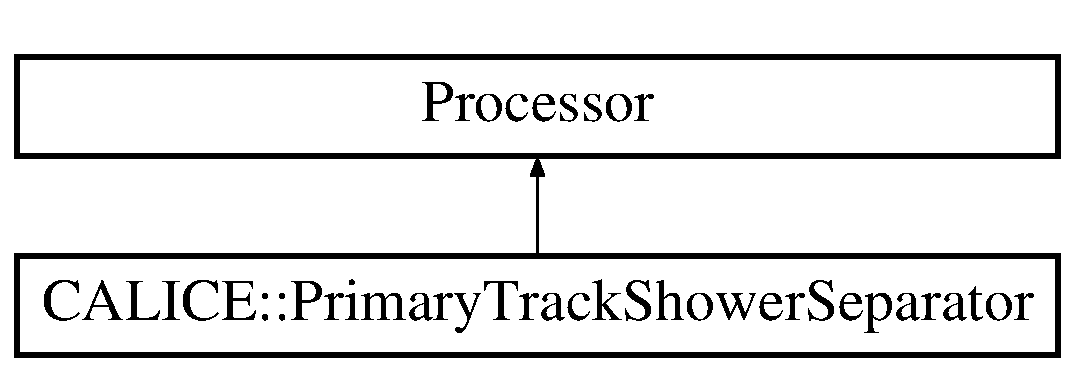
\includegraphics[height=2.000000cm]{classCALICE_1_1PrimaryTrackShowerSeparator}
\end{center}
\end{figure}
\subsection*{Public Member Functions}
\begin{DoxyCompactItemize}
\item 
{\bf Primary\-Track\-Shower\-Separator} ()
\item 
{\bf $\sim$\-Primary\-Track\-Shower\-Separator} ()
\item 
{\bf Primary\-Track\-Shower\-Separator} $\ast$ {\bfseries new\-Processor} ()\label{classCALICE_1_1PrimaryTrackShowerSeparator_a0c28aa53521cd9f6306751b9ef2f4a55}

\item 
virtual void {\bfseries init} ()\label{classCALICE_1_1PrimaryTrackShowerSeparator_a3ea401e96f08fddcd03ecd3903708703}

\item 
virtual void {\bfseries process\-Run\-Header} (L\-C\-Run\-Header $\ast$run)\label{classCALICE_1_1PrimaryTrackShowerSeparator_a1cfef7e3a39764085f4ac8462fda3dcc}

\item 
virtual void {\bfseries process\-Event} (L\-C\-Event $\ast$evt)\label{classCALICE_1_1PrimaryTrackShowerSeparator_a18b9dbb2f378118f96b5c5e9e708a9dc}

\item 
virtual void {\bfseries check} (L\-C\-Event $\ast$evt)\label{classCALICE_1_1PrimaryTrackShowerSeparator_ac3ac94e821a7851e21b7dc21e7e5d862}

\item 
virtual void {\bfseries end} ()\label{classCALICE_1_1PrimaryTrackShowerSeparator_a59af8af15c584e14c4645b07fab68a54}

\item 
virtual void {\bfseries print\-Parameters} ()\label{classCALICE_1_1PrimaryTrackShowerSeparator_a871bc0ccae1e35399194edeee9ba087e}

\end{DoxyCompactItemize}
\subsection*{Protected Attributes}
\begin{DoxyCompactItemize}
\item 
std\-::string {\bfseries \-\_\-hit\-In\-Col\-Name}\label{classCALICE_1_1PrimaryTrackShowerSeparator_aae37b56f486054d6bf8cc850ed2daece}

\item 
std\-::string {\bfseries \-\_\-evt\-Var\-Col\-Name}\label{classCALICE_1_1PrimaryTrackShowerSeparator_a069ad5d3e90a46ec690737055253f66f}

\item 
float {\bfseries \-\_\-cogradius}\label{classCALICE_1_1PrimaryTrackShowerSeparator_a9c1f1d8fa911ce06d1bae8ae5cd3272a}

\item 
float {\bfseries \-\_\-upperenergy}\label{classCALICE_1_1PrimaryTrackShowerSeparator_aeb52ab8ac8dd45c604e91060568d0c7d}

\item 
bool {\bfseries \-\_\-stminus1}\label{classCALICE_1_1PrimaryTrackShowerSeparator_aef0aa21e760270dfe10ab54b8500a3f3}

\item 
std\-::string {\bfseries \-\_\-prtrack\-Col\-Name}\label{classCALICE_1_1PrimaryTrackShowerSeparator_ade398526c8b1eb0bb61e38838d4e5c16}

\item 
std\-::string {\bfseries \-\_\-start\-Col\-Name}\label{classCALICE_1_1PrimaryTrackShowerSeparator_af22502ff2893f9f93a66a5b0accf0945}

\item 
C\-A\-L\-I\-C\-E\-::\-Mapped\-Container\\*
$<$ C\-A\-L\-I\-C\-E\-::\-Cell\-Description $>$ $\ast$ {\bfseries \-\_\-cell\-Descriptions}\label{classCALICE_1_1PrimaryTrackShowerSeparator_ac5fc5f57321c8c06d64504d0526edfbf}

\item 
int {\bf \-\_\-n\-Run}
\item 
int {\bf \-\_\-n\-Evt}
\end{DoxyCompactItemize}


\subsection{Constructor \& Destructor Documentation}
\index{C\-A\-L\-I\-C\-E\-::\-Primary\-Track\-Shower\-Separator@{C\-A\-L\-I\-C\-E\-::\-Primary\-Track\-Shower\-Separator}!Primary\-Track\-Shower\-Separator@{Primary\-Track\-Shower\-Separator}}
\index{Primary\-Track\-Shower\-Separator@{Primary\-Track\-Shower\-Separator}!CALICE::PrimaryTrackShowerSeparator@{C\-A\-L\-I\-C\-E\-::\-Primary\-Track\-Shower\-Separator}}
\subsubsection[{Primary\-Track\-Shower\-Separator}]{\setlength{\rightskip}{0pt plus 5cm}C\-A\-L\-I\-C\-E\-::\-Primary\-Track\-Shower\-Separator\-::\-Primary\-Track\-Shower\-Separator (
\begin{DoxyParamCaption}
{}
\end{DoxyParamCaption}
)}\label{classCALICE_1_1PrimaryTrackShowerSeparator_ae961d682e8a977e1d7b9ce454177bb72}
Default constructor \index{C\-A\-L\-I\-C\-E\-::\-Primary\-Track\-Shower\-Separator@{C\-A\-L\-I\-C\-E\-::\-Primary\-Track\-Shower\-Separator}!$\sim$\-Primary\-Track\-Shower\-Separator@{$\sim$\-Primary\-Track\-Shower\-Separator}}
\index{$\sim$\-Primary\-Track\-Shower\-Separator@{$\sim$\-Primary\-Track\-Shower\-Separator}!CALICE::PrimaryTrackShowerSeparator@{C\-A\-L\-I\-C\-E\-::\-Primary\-Track\-Shower\-Separator}}
\subsubsection[{$\sim$\-Primary\-Track\-Shower\-Separator}]{\setlength{\rightskip}{0pt plus 5cm}C\-A\-L\-I\-C\-E\-::\-Primary\-Track\-Shower\-Separator\-::$\sim$\-Primary\-Track\-Shower\-Separator (
\begin{DoxyParamCaption}
{}
\end{DoxyParamCaption}
)\hspace{0.3cm}{\ttfamily [inline]}}\label{classCALICE_1_1PrimaryTrackShowerSeparator_a153f317b52f741a6a530ec83edadee13}
Default destructor 

\subsection{Member Data Documentation}
\index{C\-A\-L\-I\-C\-E\-::\-Primary\-Track\-Shower\-Separator@{C\-A\-L\-I\-C\-E\-::\-Primary\-Track\-Shower\-Separator}!\-\_\-n\-Evt@{\-\_\-n\-Evt}}
\index{\-\_\-n\-Evt@{\-\_\-n\-Evt}!CALICE::PrimaryTrackShowerSeparator@{C\-A\-L\-I\-C\-E\-::\-Primary\-Track\-Shower\-Separator}}
\subsubsection[{\-\_\-n\-Evt}]{\setlength{\rightskip}{0pt plus 5cm}int C\-A\-L\-I\-C\-E\-::\-Primary\-Track\-Shower\-Separator\-::\-\_\-n\-Evt\hspace{0.3cm}{\ttfamily [protected]}}\label{classCALICE_1_1PrimaryTrackShowerSeparator_a44574d0594af56160449b808c651d0ef}
evt number \index{C\-A\-L\-I\-C\-E\-::\-Primary\-Track\-Shower\-Separator@{C\-A\-L\-I\-C\-E\-::\-Primary\-Track\-Shower\-Separator}!\-\_\-n\-Run@{\-\_\-n\-Run}}
\index{\-\_\-n\-Run@{\-\_\-n\-Run}!CALICE::PrimaryTrackShowerSeparator@{C\-A\-L\-I\-C\-E\-::\-Primary\-Track\-Shower\-Separator}}
\subsubsection[{\-\_\-n\-Run}]{\setlength{\rightskip}{0pt plus 5cm}int C\-A\-L\-I\-C\-E\-::\-Primary\-Track\-Shower\-Separator\-::\-\_\-n\-Run\hspace{0.3cm}{\ttfamily [protected]}}\label{classCALICE_1_1PrimaryTrackShowerSeparator_a47e4c719050473e3a174289c45a8ff06}
run number 

The documentation for this class was generated from the following files\-:\begin{DoxyCompactItemize}
\item 
/nfs/dust/ilc/user/marquezh/\-Calice\-Soft\-\_\-w\-\_\-\-I\-L\-C\-Soft\-\_\-v02-\/03-\/02/calice\-\_\-analysis/addon\-Procs/include/Primary\-Track\-Shower\-Separator.\-hh\item 
/nfs/dust/ilc/user/marquezh/\-Calice\-Soft\-\_\-w\-\_\-\-I\-L\-C\-Soft\-\_\-v02-\/03-\/02/calice\-\_\-analysis/addon\-Procs/src/Primary\-Track\-Shower\-Separator.\-cc\end{DoxyCompactItemize}

\section{C\-A\-L\-I\-C\-E\-:\-:Remove\-Bad\-Cells Class Reference}
\label{classCALICE_1_1RemoveBadCells}\index{C\-A\-L\-I\-C\-E\-::\-Remove\-Bad\-Cells@{C\-A\-L\-I\-C\-E\-::\-Remove\-Bad\-Cells}}


{\ttfamily \#include $<$Remove\-Bad\-Cells.\-hh$>$}

Inheritance diagram for C\-A\-L\-I\-C\-E\-:\-:Remove\-Bad\-Cells\-:\begin{figure}[H]
\begin{center}
\leavevmode
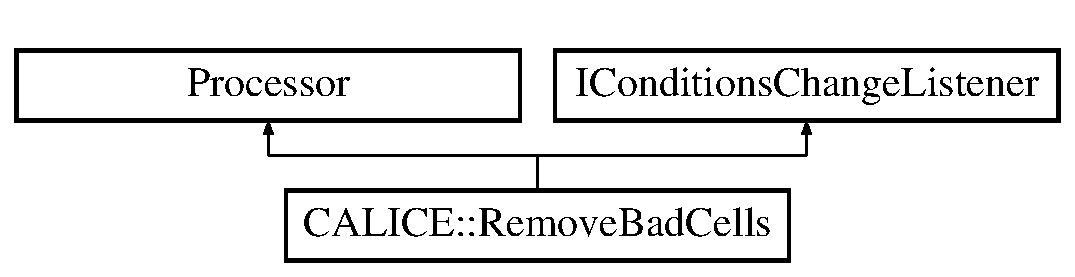
\includegraphics[height=2.000000cm]{classCALICE_1_1RemoveBadCells}
\end{center}
\end{figure}
\subsection*{Public Member Functions}
\begin{DoxyCompactItemize}
\item 
Processor $\ast$ {\bfseries new\-Processor} ()\label{classCALICE_1_1RemoveBadCells_a9788e160675b264d91fe6f423061a925}

\item 
void {\bf init} ()
\item 
void {\bf process\-Run\-Header} (L\-C\-Run\-Header $\ast$run)
\item 
void {\bf process\-Event} (L\-C\-Event $\ast$evt)
\item 
void {\bf end} ()
\item 
virtual void {\bfseries conditions\-Changed} (L\-C\-Collection $\ast$col)\label{classCALICE_1_1RemoveBadCells_abbc5dd5734b98c7db502fa6686a0b93a}

\end{DoxyCompactItemize}


\subsection{Detailed Description}
Processor which drops all hits listed in collection of Cell\-I\-Ds for bad cells from hit collection.

\begin{DoxyAuthor}{Author}
{\tt Nils.\-Feege@desy.\-de} 
\end{DoxyAuthor}
\begin{DoxyDate}{Date}
Aug 2010 
\end{DoxyDate}


\subsection{Member Function Documentation}
\index{C\-A\-L\-I\-C\-E\-::\-Remove\-Bad\-Cells@{C\-A\-L\-I\-C\-E\-::\-Remove\-Bad\-Cells}!end@{end}}
\index{end@{end}!CALICE::RemoveBadCells@{C\-A\-L\-I\-C\-E\-::\-Remove\-Bad\-Cells}}
\subsubsection[{end}]{\setlength{\rightskip}{0pt plus 5cm}void C\-A\-L\-I\-C\-E\-::\-Remove\-Bad\-Cells\-::end (
\begin{DoxyParamCaption}
{}
\end{DoxyParamCaption}
)}\label{classCALICE_1_1RemoveBadCells_a408d54223072fbc8e15d9274eeeebc9a}
Called after data processing for clean up. \index{C\-A\-L\-I\-C\-E\-::\-Remove\-Bad\-Cells@{C\-A\-L\-I\-C\-E\-::\-Remove\-Bad\-Cells}!init@{init}}
\index{init@{init}!CALICE::RemoveBadCells@{C\-A\-L\-I\-C\-E\-::\-Remove\-Bad\-Cells}}
\subsubsection[{init}]{\setlength{\rightskip}{0pt plus 5cm}void C\-A\-L\-I\-C\-E\-::\-Remove\-Bad\-Cells\-::init (
\begin{DoxyParamCaption}
{}
\end{DoxyParamCaption}
)}\label{classCALICE_1_1RemoveBadCells_a29d65f8e9b2c445a641f2ad9009b34fd}
Called at the begin of the job before anything is read. Use to initialize the processor, e.\-g. book histograms. \index{C\-A\-L\-I\-C\-E\-::\-Remove\-Bad\-Cells@{C\-A\-L\-I\-C\-E\-::\-Remove\-Bad\-Cells}!process\-Event@{process\-Event}}
\index{process\-Event@{process\-Event}!CALICE::RemoveBadCells@{C\-A\-L\-I\-C\-E\-::\-Remove\-Bad\-Cells}}
\subsubsection[{process\-Event}]{\setlength{\rightskip}{0pt plus 5cm}void C\-A\-L\-I\-C\-E\-::\-Remove\-Bad\-Cells\-::process\-Event (
\begin{DoxyParamCaption}
\item[{L\-C\-Event $\ast$}]{evt}
\end{DoxyParamCaption}
)}\label{classCALICE_1_1RemoveBadCells_a23c78e45e3b2c63345af838a5d69db03}
Called for every event -\/ this is where the real action is taking place. \index{C\-A\-L\-I\-C\-E\-::\-Remove\-Bad\-Cells@{C\-A\-L\-I\-C\-E\-::\-Remove\-Bad\-Cells}!process\-Run\-Header@{process\-Run\-Header}}
\index{process\-Run\-Header@{process\-Run\-Header}!CALICE::RemoveBadCells@{C\-A\-L\-I\-C\-E\-::\-Remove\-Bad\-Cells}}
\subsubsection[{process\-Run\-Header}]{\setlength{\rightskip}{0pt plus 5cm}void C\-A\-L\-I\-C\-E\-::\-Remove\-Bad\-Cells\-::process\-Run\-Header (
\begin{DoxyParamCaption}
\item[{L\-C\-Run\-Header $\ast$}]{run}
\end{DoxyParamCaption}
)}\label{classCALICE_1_1RemoveBadCells_aa49477acfd2b124f996126500943f51a}
Called for every run, e.\-g. overwrite to initialize run dependent histograms. 

The documentation for this class was generated from the following files\-:\begin{DoxyCompactItemize}
\item 
/nfs/dust/ilc/user/marquezh/\-Calice\-Soft\-\_\-w\-\_\-\-I\-L\-C\-Soft\-\_\-v02-\/03-\/02/calice\-\_\-analysis/addon\-Procs/include/Remove\-Bad\-Cells.\-hh\item 
/nfs/dust/ilc/user/marquezh/\-Calice\-Soft\-\_\-w\-\_\-\-I\-L\-C\-Soft\-\_\-v02-\/03-\/02/calice\-\_\-analysis/addon\-Procs/src/Remove\-Bad\-Cells.\-cc\end{DoxyCompactItemize}

\section{C\-A\-L\-I\-C\-E\-:\-:Event\-List\-Processor\-:\-:Run\-Event Struct Reference}
\label{structCALICE_1_1EventListProcessor_1_1RunEvent}\index{C\-A\-L\-I\-C\-E\-::\-Event\-List\-Processor\-::\-Run\-Event@{C\-A\-L\-I\-C\-E\-::\-Event\-List\-Processor\-::\-Run\-Event}}
\subsection*{Public Member Functions}
\begin{DoxyCompactItemize}
\item 
{\bfseries Run\-Event} (int a\-Run, int a\-Event)\label{structCALICE_1_1EventListProcessor_1_1RunEvent_a2117bde5cb5ead53a8daf77ed193f3e9}

\end{DoxyCompactItemize}
\subsection*{Public Attributes}
\begin{DoxyCompactItemize}
\item 
int {\bfseries run}\label{structCALICE_1_1EventListProcessor_1_1RunEvent_aa9b0c155d4cf3ea9d147cbabc3a79447}

\item 
int {\bfseries event}\label{structCALICE_1_1EventListProcessor_1_1RunEvent_a40064a67f8e051319bd72a269763414b}

\end{DoxyCompactItemize}


The documentation for this struct was generated from the following file\-:\begin{DoxyCompactItemize}
\item 
/nfs/dust/ilc/user/marquezh/\-Calice\-Soft\-\_\-w\-\_\-\-I\-L\-C\-Soft\-\_\-v02-\/03-\/02/calice\-\_\-analysis/addon\-Procs/include/Event\-List\-Processor.\-hh\end{DoxyCompactItemize}

\section{marlin\-:\-:Sc\-E\-C\-A\-L\-Electron\-Analysis\-Template Class Reference}
\label{classmarlin_1_1ScECALElectronAnalysisTemplate}\index{marlin\-::\-Sc\-E\-C\-A\-L\-Electron\-Analysis\-Template@{marlin\-::\-Sc\-E\-C\-A\-L\-Electron\-Analysis\-Template}}
Inheritance diagram for marlin\-:\-:Sc\-E\-C\-A\-L\-Electron\-Analysis\-Template\-:\begin{figure}[H]
\begin{center}
\leavevmode
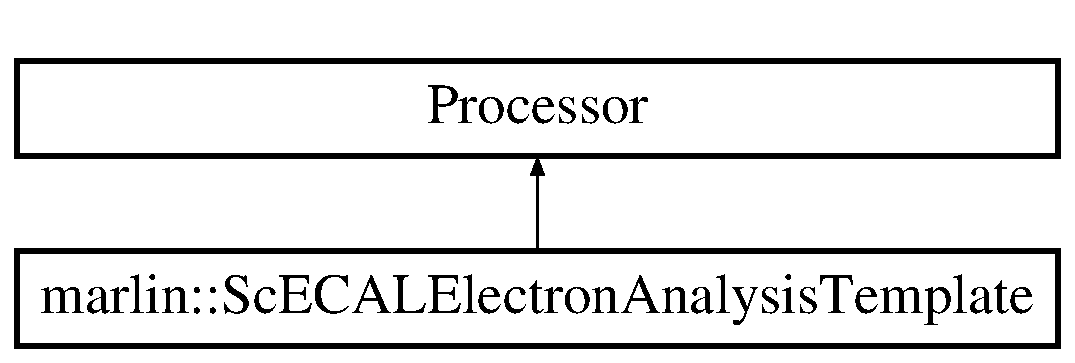
\includegraphics[height=2.000000cm]{classmarlin_1_1ScECALElectronAnalysisTemplate}
\end{center}
\end{figure}
\subsection*{Public Member Functions}
\begin{DoxyCompactItemize}
\item 
virtual Processor $\ast$ {\bfseries new\-Processor} ()\label{classmarlin_1_1ScECALElectronAnalysisTemplate_adc4c17bb572996cc483589511f367da2}

\item 
virtual void {\bfseries init} ()\label{classmarlin_1_1ScECALElectronAnalysisTemplate_a1c4fa55164dd262bdfeb9fd1b7a0a55b}

\item 
virtual void {\bf process\-Event} (L\-C\-Event $\ast$evt)
\item 
virtual void {\bfseries end} ()\label{classmarlin_1_1ScECALElectronAnalysisTemplate_a2165411c184cc37119c3c944ecd82744}

\end{DoxyCompactItemize}


\subsection{Member Function Documentation}
\index{marlin\-::\-Sc\-E\-C\-A\-L\-Electron\-Analysis\-Template@{marlin\-::\-Sc\-E\-C\-A\-L\-Electron\-Analysis\-Template}!process\-Event@{process\-Event}}
\index{process\-Event@{process\-Event}!marlin::ScECALElectronAnalysisTemplate@{marlin\-::\-Sc\-E\-C\-A\-L\-Electron\-Analysis\-Template}}
\subsubsection[{process\-Event}]{\setlength{\rightskip}{0pt plus 5cm}void marlin\-::\-Sc\-E\-C\-A\-L\-Electron\-Analysis\-Template\-::process\-Event (
\begin{DoxyParamCaption}
\item[{L\-C\-Event $\ast$}]{evt}
\end{DoxyParamCaption}
)\hspace{0.3cm}{\ttfamily [virtual]}}\label{classmarlin_1_1ScECALElectronAnalysisTemplate_a3626f4fc4d083204f226e55a08e136cc}
the end of E\-C\-A\-L hits loop 

The documentation for this class was generated from the following files\-:\begin{DoxyCompactItemize}
\item 
/nfs/dust/ilc/user/marquezh/\-Calice\-Soft\-\_\-w\-\_\-\-I\-L\-C\-Soft\-\_\-v02-\/03-\/02/calice\-\_\-analysis/addon\-Procs/include/Sc\-E\-C\-A\-L\-Electron\-Analysis\-Template.\-hh\item 
/nfs/dust/ilc/user/marquezh/\-Calice\-Soft\-\_\-w\-\_\-\-I\-L\-C\-Soft\-\_\-v02-\/03-\/02/calice\-\_\-analysis/addon\-Procs/src/Sc\-E\-C\-A\-L\-Electron\-Analysis\-Template.\-cc\end{DoxyCompactItemize}

\section{C\-A\-L\-I\-C\-E\-:\-:Shower\-Start\-Cluster\-Processor Class Reference}
\label{classCALICE_1_1ShowerStartClusterProcessor}\index{C\-A\-L\-I\-C\-E\-::\-Shower\-Start\-Cluster\-Processor@{C\-A\-L\-I\-C\-E\-::\-Shower\-Start\-Cluster\-Processor}}
Inheritance diagram for C\-A\-L\-I\-C\-E\-:\-:Shower\-Start\-Cluster\-Processor\-:\begin{figure}[H]
\begin{center}
\leavevmode
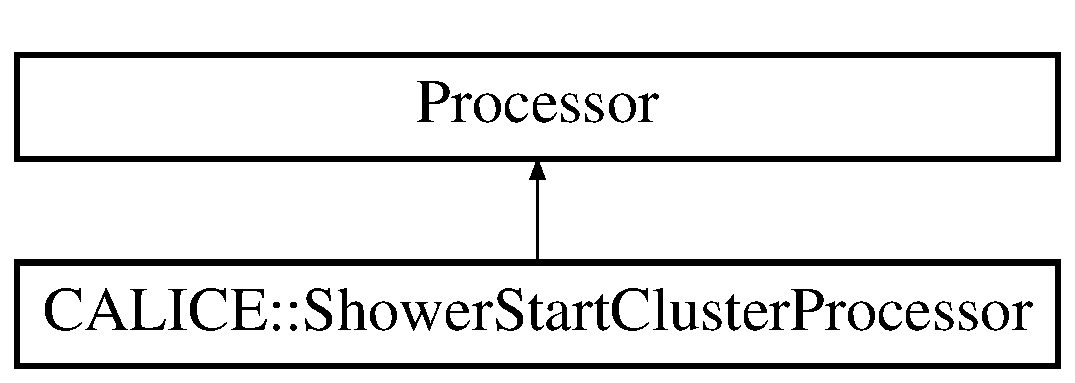
\includegraphics[height=2.000000cm]{classCALICE_1_1ShowerStartClusterProcessor}
\end{center}
\end{figure}
\subsection*{Public Member Functions}
\begin{DoxyCompactItemize}
\item 
virtual Processor $\ast$ {\bfseries new\-Processor} ()\label{classCALICE_1_1ShowerStartClusterProcessor_a9b12a2d0ab6adbb8a53cbce140594591}

\item 
virtual void {\bfseries init} ()\label{classCALICE_1_1ShowerStartClusterProcessor_adf7a5d49de5ce05ddab35a2fdf619639}

\item 
virtual void {\bfseries process\-Run\-Header} (L\-C\-Run\-Header $\ast$run)\label{classCALICE_1_1ShowerStartClusterProcessor_a34a2a0630e0c6ae47f49c2f49c76ea08}

\item 
virtual void {\bfseries process\-Event} (L\-C\-Event $\ast$evt)\label{classCALICE_1_1ShowerStartClusterProcessor_a13772a5bcf8f8a57796ea314e605a21d}

\item 
virtual void {\bfseries end} ()\label{classCALICE_1_1ShowerStartClusterProcessor_ae5de75e169db59ebf3899fbd625c1431}

\end{DoxyCompactItemize}


The documentation for this class was generated from the following files\-:\begin{DoxyCompactItemize}
\item 
/nfs/dust/ilc/user/marquezh/\-Calice\-Soft\-\_\-w\-\_\-\-I\-L\-C\-Soft\-\_\-v02-\/03-\/02/calice\-\_\-analysis/addon\-Procs/include/Shower\-Start\-Cluster\-Processor.\-hh\item 
/nfs/dust/ilc/user/marquezh/\-Calice\-Soft\-\_\-w\-\_\-\-I\-L\-C\-Soft\-\_\-v02-\/03-\/02/calice\-\_\-analysis/addon\-Procs/src/Shower\-Start\-Cluster\-Processor.\-cc\end{DoxyCompactItemize}

\section{C\-A\-L\-I\-C\-E\-:\-:Shower\-Start\-Finding\-Processor Class Reference}
\label{classCALICE_1_1ShowerStartFindingProcessor}\index{C\-A\-L\-I\-C\-E\-::\-Shower\-Start\-Finding\-Processor@{C\-A\-L\-I\-C\-E\-::\-Shower\-Start\-Finding\-Processor}}
Inheritance diagram for C\-A\-L\-I\-C\-E\-:\-:Shower\-Start\-Finding\-Processor\-:\begin{figure}[H]
\begin{center}
\leavevmode
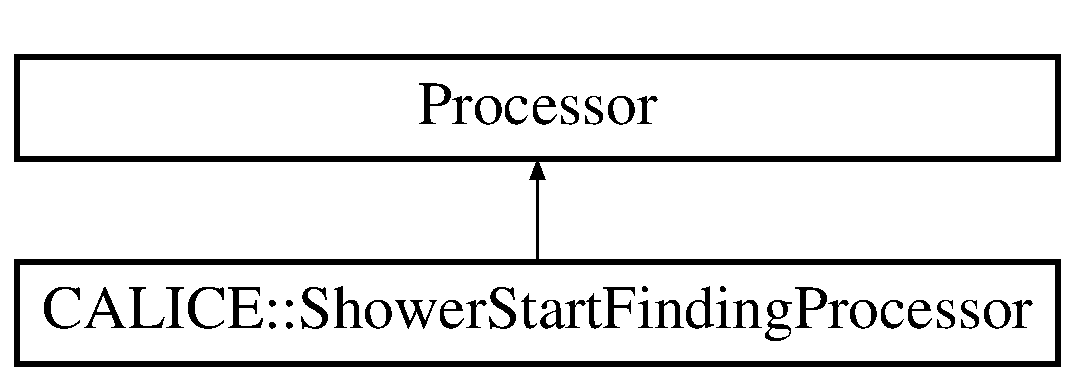
\includegraphics[height=2.000000cm]{classCALICE_1_1ShowerStartFindingProcessor}
\end{center}
\end{figure}
\subsection*{Public Member Functions}
\begin{DoxyCompactItemize}
\item 
virtual Processor $\ast$ {\bfseries new\-Processor} ()\label{classCALICE_1_1ShowerStartFindingProcessor_a9979ef5ecce85c879ecf7157ad335f58}

\item 
virtual void {\bfseries init} ()\label{classCALICE_1_1ShowerStartFindingProcessor_a7b7a9d43bdf70d4193f47581f25d17d8}

\item 
virtual void {\bfseries process\-Run\-Header} (L\-C\-Run\-Header $\ast$run)\label{classCALICE_1_1ShowerStartFindingProcessor_ace5d5ba7c39f51105b227fa72b953042}

\item 
virtual void {\bfseries process\-Event} (L\-C\-Event $\ast$evt)\label{classCALICE_1_1ShowerStartFindingProcessor_a20017eb87e4d5e1d536b67ae3f329ebb}

\item 
virtual void {\bfseries check} (L\-C\-Event $\ast$evt)\label{classCALICE_1_1ShowerStartFindingProcessor_a4fb687725d5e96acb2081bf67576e133}

\item 
virtual void {\bfseries end} ()\label{classCALICE_1_1ShowerStartFindingProcessor_afb3a8ab953345eb81b7586e4838fa429}

\item 
virtual void {\bfseries print\-Parameters} ()\label{classCALICE_1_1ShowerStartFindingProcessor_ab183bd3b80736e55b060a114b98a8abb}

\end{DoxyCompactItemize}
\subsection*{Protected Attributes}
\begin{DoxyCompactItemize}
\item 
std\-::string {\bfseries \-\_\-hit\-In\-Col\-Name}\label{classCALICE_1_1ShowerStartFindingProcessor_a9c50821b58ba551c15361bfae4c240ef}

\item 
std\-::string {\bfseries \-\_\-evt\-Var\-Col\-Name}\label{classCALICE_1_1ShowerStartFindingProcessor_a5cfc455dcb59c246607ed5b0dfce5c75}

\item 
std\-::string {\bfseries \-\_\-lay\-Var\-Col\-Name}\label{classCALICE_1_1ShowerStartFindingProcessor_a58c3524ed8a79759488b0d98358a94ab}

\item 
std\-::string {\bfseries \-\_\-hit\-Var\-Col\-Name}\label{classCALICE_1_1ShowerStartFindingProcessor_a0eee5d368488730f3589e961330711a7}

\item 
float {\bfseries \-\_\-beam\-Energy}\label{classCALICE_1_1ShowerStartFindingProcessor_ae456e97022ca26ff92197c9565ada3bd}

\item 
float {\bfseries \-\_\-correction\-M\-I\-Pcrit}\label{classCALICE_1_1ShowerStartFindingProcessor_a6b7b733b0f842427753dd67cb88289a4}

\item 
int {\bfseries \-\_\-win\-\_\-mov\-\_\-av}\label{classCALICE_1_1ShowerStartFindingProcessor_ab0330e51ef694eeb9a30224ad0f3ac57}

\item 
bool {\bfseries \-\_\-muon\-Crit\-Flag}\label{classCALICE_1_1ShowerStartFindingProcessor_afa13e374ba8199edcd6532fa5f275b67}

\item 
bool {\bfseries \-\_\-is\-T\-B\-May18}\label{classCALICE_1_1ShowerStartFindingProcessor_a254c351165697fa527745ce22b6f9f6b}

\item 
bool {\bfseries \-\_\-is\-T\-B\-June18}\label{classCALICE_1_1ShowerStartFindingProcessor_a6a5e06076b811969435484f48cca68d6}

\item 
bool {\bfseries \-\_\-\-Legacy\-\_\-\-S\-S\-F\-\_\-\-Thresholds}\label{classCALICE_1_1ShowerStartFindingProcessor_a381c0af0673aa5b3036ec4de30185a08}

\item 
float {\bfseries \-\_\-muon\-Crit\-Threshold}\label{classCALICE_1_1ShowerStartFindingProcessor_a066b28ed7384246a9562247c5fddcee4}

\item 
int {\bfseries \-\_\-\-M\-I\-P2\-Ge\-V\-Flag}\label{classCALICE_1_1ShowerStartFindingProcessor_a267cc5b391e7cdf1f656ce4cfbf5b454}

\item 
float {\bfseries \-\_\-\-M\-I\-P2\-Ge\-V\-Factor}\label{classCALICE_1_1ShowerStartFindingProcessor_a7c989a2d5f1ea4770c3a0612eda6d5a5}

\item 
int {\bf \-\_\-n\-Run}
\item 
int {\bf \-\_\-n\-Evt}
\end{DoxyCompactItemize}


\subsection{Member Data Documentation}
\index{C\-A\-L\-I\-C\-E\-::\-Shower\-Start\-Finding\-Processor@{C\-A\-L\-I\-C\-E\-::\-Shower\-Start\-Finding\-Processor}!\-\_\-n\-Evt@{\-\_\-n\-Evt}}
\index{\-\_\-n\-Evt@{\-\_\-n\-Evt}!CALICE::ShowerStartFindingProcessor@{C\-A\-L\-I\-C\-E\-::\-Shower\-Start\-Finding\-Processor}}
\subsubsection[{\-\_\-n\-Evt}]{\setlength{\rightskip}{0pt plus 5cm}int C\-A\-L\-I\-C\-E\-::\-Shower\-Start\-Finding\-Processor\-::\-\_\-n\-Evt\hspace{0.3cm}{\ttfamily [protected]}}\label{classCALICE_1_1ShowerStartFindingProcessor_a72c7d1f00d408a32614f91212cd900f1}
evt number \index{C\-A\-L\-I\-C\-E\-::\-Shower\-Start\-Finding\-Processor@{C\-A\-L\-I\-C\-E\-::\-Shower\-Start\-Finding\-Processor}!\-\_\-n\-Run@{\-\_\-n\-Run}}
\index{\-\_\-n\-Run@{\-\_\-n\-Run}!CALICE::ShowerStartFindingProcessor@{C\-A\-L\-I\-C\-E\-::\-Shower\-Start\-Finding\-Processor}}
\subsubsection[{\-\_\-n\-Run}]{\setlength{\rightskip}{0pt plus 5cm}int C\-A\-L\-I\-C\-E\-::\-Shower\-Start\-Finding\-Processor\-::\-\_\-n\-Run\hspace{0.3cm}{\ttfamily [protected]}}\label{classCALICE_1_1ShowerStartFindingProcessor_a99b1ddb20243bd7f438522b8d9f3da0e}
run number 

The documentation for this class was generated from the following files\-:\begin{DoxyCompactItemize}
\item 
/nfs/dust/ilc/user/marquezh/\-Calice\-Soft\-\_\-w\-\_\-\-I\-L\-C\-Soft\-\_\-v02-\/03-\/02/calice\-\_\-analysis/addon\-Procs/include/Shower\-Start\-Finding\-Processor.\-hh\item 
/nfs/dust/ilc/user/marquezh/\-Calice\-Soft\-\_\-w\-\_\-\-I\-L\-C\-Soft\-\_\-v02-\/03-\/02/calice\-\_\-analysis/addon\-Procs/src/Shower\-Start\-Finding\-Processor.\-cc\end{DoxyCompactItemize}

\section{C\-A\-L\-I\-C\-E\-:\-:Sort\-By\-Z\-Position Class Reference}
\label{classCALICE_1_1SortByZPosition}\index{C\-A\-L\-I\-C\-E\-::\-Sort\-By\-Z\-Position@{C\-A\-L\-I\-C\-E\-::\-Sort\-By\-Z\-Position}}
\subsection*{Public Member Functions}
\begin{DoxyCompactItemize}
\item 
bool {\bfseries operator()} (const Calorimeter\-Hit $\ast$hit, const Calorimeter\-Hit $\ast$ref)\label{classCALICE_1_1SortByZPosition_af4abe2bd8768d6be11fa7f67e93ea37e}

\end{DoxyCompactItemize}


The documentation for this class was generated from the following files\-:\begin{DoxyCompactItemize}
\item 
/nfs/dust/ilc/user/marquezh/\-Calice\-Soft\-\_\-w\-\_\-\-I\-L\-C\-Soft\-\_\-v02-\/03-\/02/calice\-\_\-analysis/addon\-Procs/include/Shower\-Start\-Cluster\-Processor.\-hh\item 
/nfs/dust/ilc/user/marquezh/\-Calice\-Soft\-\_\-w\-\_\-\-I\-L\-C\-Soft\-\_\-v02-\/03-\/02/calice\-\_\-analysis/addon\-Procs/src/Shower\-Start\-Cluster\-Processor.\-cc\end{DoxyCompactItemize}

\section{C\-A\-L\-I\-C\-E\-:\-:Std\-Variables\-Processor Class Reference}
\label{classCALICE_1_1StdVariablesProcessor}\index{C\-A\-L\-I\-C\-E\-::\-Std\-Variables\-Processor@{C\-A\-L\-I\-C\-E\-::\-Std\-Variables\-Processor}}
Inheritance diagram for C\-A\-L\-I\-C\-E\-:\-:Std\-Variables\-Processor\-:\begin{figure}[H]
\begin{center}
\leavevmode
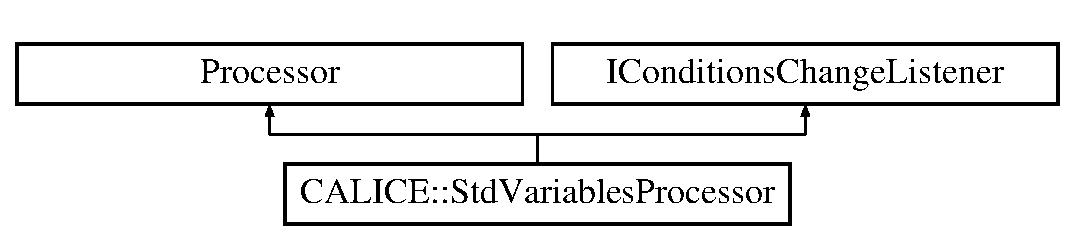
\includegraphics[height=2.000000cm]{classCALICE_1_1StdVariablesProcessor}
\end{center}
\end{figure}
\subsection*{Public Member Functions}
\begin{DoxyCompactItemize}
\item 
virtual Processor $\ast$ {\bfseries new\-Processor} ()\label{classCALICE_1_1StdVariablesProcessor_aa96a51dd44cc70d52fcd1df10a55f331}

\item 
virtual void {\bfseries init} ()\label{classCALICE_1_1StdVariablesProcessor_abe716dde8244653669e7c4990eab105c}

\item 
virtual void {\bfseries process\-Run\-Header} (L\-C\-Run\-Header $\ast$run)\label{classCALICE_1_1StdVariablesProcessor_a75e89ae7de63ceddc90cf7d1284c2dae}

\item 
virtual void {\bfseries process\-Event} (L\-C\-Event $\ast$evt)\label{classCALICE_1_1StdVariablesProcessor_a4ea9c975b691ae469f446c9d3f36fd42}

\item 
virtual void {\bfseries check} (L\-C\-Event $\ast$evt)\label{classCALICE_1_1StdVariablesProcessor_ad1643b0238a809f4f7d7bba4015d28b1}

\item 
virtual void {\bfseries end} ()\label{classCALICE_1_1StdVariablesProcessor_a8e967ab99bb311497528e77b70f5a446}

\item 
virtual void {\bfseries print\-Parameters} ()\label{classCALICE_1_1StdVariablesProcessor_afded2068fe77768100f667b0726bc4ca}

\item 
virtual void {\bfseries conditions\-Changed} (L\-C\-Collection $\ast$col)\label{classCALICE_1_1StdVariablesProcessor_a87d58f394dd0abf0c881ceed6625b3b8}

\end{DoxyCompactItemize}
\subsection*{Protected Attributes}
\begin{DoxyCompactItemize}
\item 
std\-::string {\bfseries \-\_\-hit\-In\-Col\-Name}\label{classCALICE_1_1StdVariablesProcessor_aadc6a49bb1e52a556f5ea399c9109e37}

\item 
std\-::string {\bfseries \-\_\-hit\-Out\-Col\-Name}\label{classCALICE_1_1StdVariablesProcessor_a45016350cf5217ee91e26d0c1f65dd63}

\item 
std\-::string {\bfseries \-\_\-evtvar\-Col\-Name}\label{classCALICE_1_1StdVariablesProcessor_aa7184fe7a54cd2d14c540ff1dde40fa7}

\item 
std\-::string {\bfseries \-\_\-layvar\-Col\-Name}\label{classCALICE_1_1StdVariablesProcessor_a2603f6c8b008cc1664085639d2d126e4}

\item 
std\-::string {\bfseries \-\_\-hitvar\-Col\-Name}\label{classCALICE_1_1StdVariablesProcessor_a1ed0c7668fb83ef5f9d8809d8dd92928}

\item 
std\-::string {\bfseries \-\_\-layer\-Var2\-Cal\-Hit\-Col\-Name}\label{classCALICE_1_1StdVariablesProcessor_ae92a6b1e7862f19928c46065a89e7261}

\item 
std\-::string {\bfseries \-\_\-cal\-Hit2\-Hit\-Var\-Col\-Name}\label{classCALICE_1_1StdVariablesProcessor_a0e63c9196e848c264f8d9ddd3d026132}

\item 
std\-::string {\bfseries \-\_\-col\-Name\-Module\-Location}\label{classCALICE_1_1StdVariablesProcessor_a66e290ab85d79c37f8ea62fead7bbbf8}

\item 
std\-::string {\bfseries \-\_\-cell\-Description\-Processor\-Name}\label{classCALICE_1_1StdVariablesProcessor_ae2f041e65e02919bcbe5c0c35873a1a8}

\item 
C\-A\-L\-I\-C\-E\-::\-Mapped\-Container\\*
$<$ C\-A\-L\-I\-C\-E\-::\-Cell\-Description $>$ $\ast$ {\bfseries \-\_\-cell\-Descriptions}\label{classCALICE_1_1StdVariablesProcessor_a1209cbdaf500094f904a5bad385c2efb}

\item 
bool {\bfseries \-\_\-module\-Location\-Changed}\label{classCALICE_1_1StdVariablesProcessor_a85d5e073ae94886a002bb3276c7ca6f1}

\item 
L\-C\-Collection $\ast$ {\bfseries \-\_\-col\-Module\-Location}\label{classCALICE_1_1StdVariablesProcessor_a947bfa01350791851bf2f4a4e7f07049}

\item 
int {\bfseries \-\_\-\-M\-I\-P2\-Ge\-V\-Flag}\label{classCALICE_1_1StdVariablesProcessor_a2eaa6e0a04c49c619121c4c1e3d34554}

\item 
float {\bfseries \-\_\-\-M\-I\-P2\-Ge\-V\-Factor}\label{classCALICE_1_1StdVariablesProcessor_a9b268ddaa721e3f513bfd64c99ccef81}

\item 
int {\bfseries \-\_\-first\-Layer\-K}\label{classCALICE_1_1StdVariablesProcessor_a46553445ca3521b4e1b03db7881de7eb}

\item 
int {\bf \-\_\-n\-Run}
\item 
int {\bf \-\_\-n\-Evt}
\end{DoxyCompactItemize}


\subsection{Member Data Documentation}
\index{C\-A\-L\-I\-C\-E\-::\-Std\-Variables\-Processor@{C\-A\-L\-I\-C\-E\-::\-Std\-Variables\-Processor}!\-\_\-n\-Evt@{\-\_\-n\-Evt}}
\index{\-\_\-n\-Evt@{\-\_\-n\-Evt}!CALICE::StdVariablesProcessor@{C\-A\-L\-I\-C\-E\-::\-Std\-Variables\-Processor}}
\subsubsection[{\-\_\-n\-Evt}]{\setlength{\rightskip}{0pt plus 5cm}int C\-A\-L\-I\-C\-E\-::\-Std\-Variables\-Processor\-::\-\_\-n\-Evt\hspace{0.3cm}{\ttfamily [protected]}}\label{classCALICE_1_1StdVariablesProcessor_af5fab38a7f311ea31545e5acd271dc48}
evt number \index{C\-A\-L\-I\-C\-E\-::\-Std\-Variables\-Processor@{C\-A\-L\-I\-C\-E\-::\-Std\-Variables\-Processor}!\-\_\-n\-Run@{\-\_\-n\-Run}}
\index{\-\_\-n\-Run@{\-\_\-n\-Run}!CALICE::StdVariablesProcessor@{C\-A\-L\-I\-C\-E\-::\-Std\-Variables\-Processor}}
\subsubsection[{\-\_\-n\-Run}]{\setlength{\rightskip}{0pt plus 5cm}int C\-A\-L\-I\-C\-E\-::\-Std\-Variables\-Processor\-::\-\_\-n\-Run\hspace{0.3cm}{\ttfamily [protected]}}\label{classCALICE_1_1StdVariablesProcessor_afe1e269790b0eeaca2eacef43d3b6307}
run number 

The documentation for this class was generated from the following files\-:\begin{DoxyCompactItemize}
\item 
/nfs/dust/ilc/user/marquezh/\-Calice\-Soft\-\_\-w\-\_\-\-I\-L\-C\-Soft\-\_\-v02-\/03-\/02/calice\-\_\-analysis/addon\-Procs/include/Std\-Variables\-Processor.\-hh\item 
/nfs/dust/ilc/user/marquezh/\-Calice\-Soft\-\_\-w\-\_\-\-I\-L\-C\-Soft\-\_\-v02-\/03-\/02/calice\-\_\-analysis/addon\-Procs/src/Std\-Variables\-Processor.\-cc\end{DoxyCompactItemize}

\section{C\-A\-L\-I\-C\-E\-:\-:T\-B\-Particle\-I\-D Class Reference}
\label{classCALICE_1_1TBParticleID}\index{C\-A\-L\-I\-C\-E\-::\-T\-B\-Particle\-I\-D@{C\-A\-L\-I\-C\-E\-::\-T\-B\-Particle\-I\-D}}
Inheritance diagram for C\-A\-L\-I\-C\-E\-:\-:T\-B\-Particle\-I\-D\-:\begin{figure}[H]
\begin{center}
\leavevmode
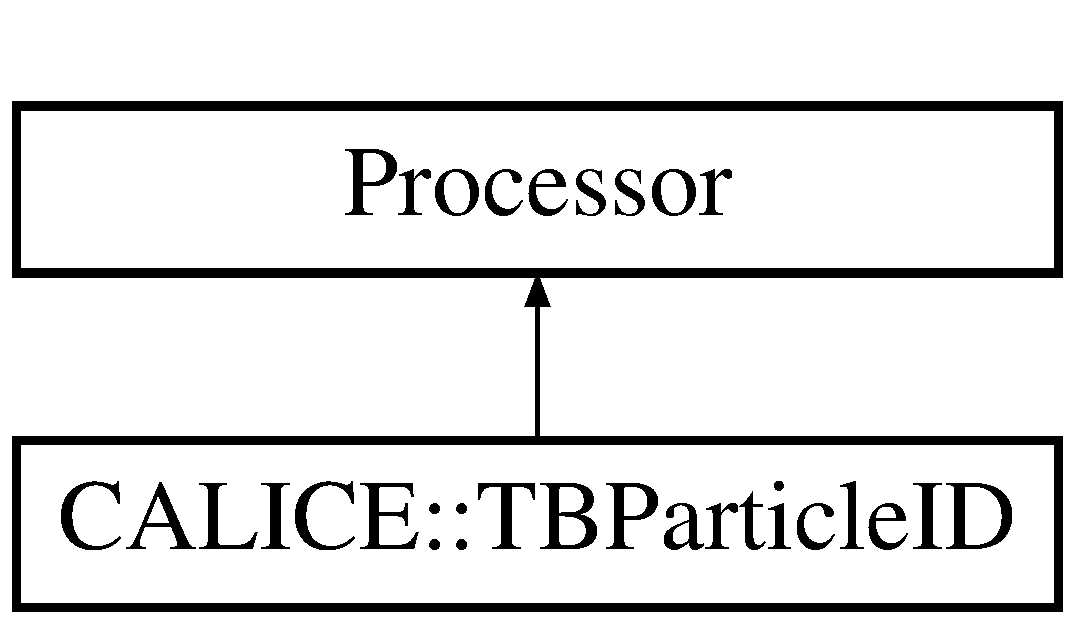
\includegraphics[height=2.000000cm]{classCALICE_1_1TBParticleID}
\end{center}
\end{figure}
\subsection*{Public Member Functions}
\begin{DoxyCompactItemize}
\item 
virtual Processor $\ast$ {\bfseries new\-Processor} ()\label{classCALICE_1_1TBParticleID_aadfd282af1f27ae3caf7dac62c2fef7d}

\item 
virtual void {\bfseries init} ()\label{classCALICE_1_1TBParticleID_a62119eec9f824b59227306e7ae8d7d8b}

\item 
virtual void {\bfseries process\-Run\-Header} (L\-C\-Run\-Header $\ast$run)\label{classCALICE_1_1TBParticleID_a76978008edc972ed71f12b712a4ede16}

\item 
virtual void {\bfseries process\-Event} (L\-C\-Event $\ast$evt)\label{classCALICE_1_1TBParticleID_a675837ef4e01e67e38333a35e57d8854}

\item 
virtual void {\bfseries check} (L\-C\-Event $\ast$evt)\label{classCALICE_1_1TBParticleID_a9a710d267d75975230465ffc3a4a6570}

\item 
virtual void {\bfseries end} ()\label{classCALICE_1_1TBParticleID_a2f27766b24eb06663e19fda0a12e72bb}

\item 
virtual void {\bfseries print\-Parameters} ()\label{classCALICE_1_1TBParticleID_a04699895d2768c48500e63c6f47ff7a2}

\end{DoxyCompactItemize}
\subsection*{Protected Member Functions}
\begin{DoxyCompactItemize}
\item 
bool {\bfseries check\-Cuts} ({\bf I\-D\-Variables} var, {\bf I\-D\-Cuts} cuts)\label{classCALICE_1_1TBParticleID_a78800c66439da5a558daf8ab9348f7d7}

\end{DoxyCompactItemize}
\subsection*{Protected Attributes}
\begin{DoxyCompactItemize}
\item 
{\bf I\-D\-Variables} {\bfseries I\-Dset}\label{classCALICE_1_1TBParticleID_af4b5bde6f0934f812d762cf9abd9dcfd}

\item 
int {\bfseries \-\_\-first\-A\-H\-C\-A\-Llayer\-K}\label{classCALICE_1_1TBParticleID_ae8984f067424aeabf28008956022247c}

\item 
bool {\bfseries \-\_\-apply\-Event\-Filtering}\label{classCALICE_1_1TBParticleID_aa254187a280d25a15c97d87fb39afbd4}

\item 
int {\bfseries \-\_\-\-I\-D\-Mode}\label{classCALICE_1_1TBParticleID_a6be651c4ff2f75af110ac1053b04734c}

\item 
int {\bfseries \-\_\-min\-Nhits}\label{classCALICE_1_1TBParticleID_ab8677ab8b866fab988c6250e76119bc1}

\item 
float {\bfseries \-\_\-radius\-Of\-Central\-Region}\label{classCALICE_1_1TBParticleID_a9737ef4957d21523e7bdc4ab3d30c325}

\item 
int {\bfseries \-\_\-n\-Last\-Layers\-For\-Muons}\label{classCALICE_1_1TBParticleID_a06a8b150c9da9dccc331a8c44a950818}

\item 
float {\bfseries \-\_\-max\-Zof\-Cluster\-Start}\label{classCALICE_1_1TBParticleID_a54759dd0fbce39fb79de313f2e0f459f}

\item 
int {\bfseries \-\_\-n\-First\-Layers}\label{classCALICE_1_1TBParticleID_abe41f40368774c27b8329c2cf569e340}

\item 
float {\bfseries \-\_\-max\-Cluster\-Spread}\label{classCALICE_1_1TBParticleID_a17558207406905a9fc632b3fe087ed60}

\item 
bool {\bfseries \-\_\-write\-I\-D\-Root}\label{classCALICE_1_1TBParticleID_a8ce610e6e3a491b2c9d16170bd257e7d}

\item 
bool {\bfseries \-\_\-write\-Cut\-Based\-I\-Dto\-Event}\label{classCALICE_1_1TBParticleID_a0029a02ec273b36da143fbe26c00e6e7}

\item 
bool {\bfseries \-\_\-manual\-Cuts}\label{classCALICE_1_1TBParticleID_a9f55cc706910a141791667a03065b1e9}

\item 
int {\bfseries \-\_\-n\-Primary\-Track\-Layers}\label{classCALICE_1_1TBParticleID_a5a9374663f7ef1289dbb17fa2f5338d6}

\item 
int {\bfseries \-\_\-min\-Hits\-In\-Primary\-Track}\label{classCALICE_1_1TBParticleID_a3de8a0e5d50e2142737d6ac60a2a7b56}

\item 
int {\bfseries \-\_\-mu\-\_\-n\-Hits\-\_\-min}\label{classCALICE_1_1TBParticleID_a793c2d6e9f029b9b72ea29a82f88b812}

\item 
int {\bfseries \-\_\-mu\-\_\-n\-Hits\-\_\-max}\label{classCALICE_1_1TBParticleID_aa23845b93c5abb51b3572af7428790e3}

\item 
int {\bfseries \-\_\-mu\-\_\-st\-\_\-min}\label{classCALICE_1_1TBParticleID_a6cb0e4575f7a716c5d8a93d97de2c101}

\item 
int {\bfseries \-\_\-mu\-\_\-st\-\_\-max}\label{classCALICE_1_1TBParticleID_a831e158c4f5a4f119c8ce05825c47778}

\item 
float {\bfseries \-\_\-mu\-\_\-zcog\-\_\-min}\label{classCALICE_1_1TBParticleID_a27922ccc3f90a610eaf17758c3a8a1b9}

\item 
float {\bfseries \-\_\-mu\-\_\-zcog\-\_\-max}\label{classCALICE_1_1TBParticleID_a4e9540cc8dec9cf6b34c20c388ba7b29}

\item 
float {\bfseries \-\_\-mu\-\_\-frac25\-\_\-min}\label{classCALICE_1_1TBParticleID_a28176b942d3fdf41b43d1f5b877f7c61}

\item 
float {\bfseries \-\_\-mu\-\_\-radius\-\_\-min}\label{classCALICE_1_1TBParticleID_a2f230b341175de64d97edd1883416ac4}

\item 
float {\bfseries \-\_\-mu\-\_\-radius\-\_\-max}\label{classCALICE_1_1TBParticleID_aa26b82ccf42ba3dcf0bec687a3d10e1e}

\item 
float {\bfseries \-\_\-mu\-\_\-e\-Sum\-\_\-min}\label{classCALICE_1_1TBParticleID_a85240822913dd38a4874b278b54a4515}

\item 
float {\bfseries \-\_\-mu\-\_\-e\-Sum\-\_\-max}\label{classCALICE_1_1TBParticleID_a14bf378a3049faaa128411d7ca4909cd}

\item 
float {\bfseries \-\_\-mu\-\_\-frac\-Track\-\_\-min}\label{classCALICE_1_1TBParticleID_aba41d284ba4ba74a66457905bbab9cf7}

\item 
int {\bfseries \-\_\-ele\-\_\-n\-Hits\-\_\-min}\label{classCALICE_1_1TBParticleID_a133152274f10743cf372c2a14367bb60}

\item 
int {\bfseries \-\_\-ele\-\_\-n\-Hits\-\_\-max}\label{classCALICE_1_1TBParticleID_a35669f94a5e3f03b3b877e37266ef98b}

\item 
int {\bfseries \-\_\-ele\-\_\-st\-\_\-min}\label{classCALICE_1_1TBParticleID_a9dd72f623cc17840248cf356219d24d1}

\item 
int {\bfseries \-\_\-ele\-\_\-st\-\_\-max}\label{classCALICE_1_1TBParticleID_a005faf75adde4f2e783d8c65cc2f6d6e}

\item 
float {\bfseries \-\_\-ele\-\_\-zcog\-\_\-min}\label{classCALICE_1_1TBParticleID_ab1613c7c91f41341cc1419eee978b8fa}

\item 
float {\bfseries \-\_\-ele\-\_\-zcog\-\_\-max}\label{classCALICE_1_1TBParticleID_a162922d980682e8436614a644c8fb021}

\item 
float {\bfseries \-\_\-ele\-\_\-frac25\-\_\-min}\label{classCALICE_1_1TBParticleID_a79d442a79ec0774526c091ac32ca25aa}

\item 
float {\bfseries \-\_\-ele\-\_\-radius\-\_\-min}\label{classCALICE_1_1TBParticleID_ab9f12845258335be4e39820a7bd55b5f}

\item 
float {\bfseries \-\_\-ele\-\_\-radius\-\_\-max}\label{classCALICE_1_1TBParticleID_a7c097f6916335c41eb0c5525fcc82d70}

\item 
float {\bfseries \-\_\-ele\-\_\-e\-Sum\-\_\-min}\label{classCALICE_1_1TBParticleID_ab3b6f511ee5652dbf565aeab418d6f03}

\item 
float {\bfseries \-\_\-ele\-\_\-e\-Sum\-\_\-max}\label{classCALICE_1_1TBParticleID_a208561b349fb4fe0851ef80bfcec713b}

\item 
float {\bfseries \-\_\-ele\-\_\-frac\-Core\-\_\-min}\label{classCALICE_1_1TBParticleID_aeb4d044983487d07a79f042de81dfc59}

\item 
float {\bfseries \-\_\-ele\-\_\-frac\-Det\-\_\-max}\label{classCALICE_1_1TBParticleID_aa1734c1630b08976098ac68a5393ed9d}

\item 
float {\bfseries \-\_\-ele\-\_\-frac\-Track\-\_\-max}\label{classCALICE_1_1TBParticleID_acfe9762e7242a023f66c3c840ebd3c96}

\item 
Booster\-Handle {\bfseries handle}\label{classCALICE_1_1TBParticleID_a30f6a7c76f4107d3e5b04c4ce2d0c5fa}

\item 
double {\bfseries classifier} [3]\label{classCALICE_1_1TBParticleID_a69e12d5fb20171f7cc67884c44613154}

\item 
bool {\bfseries \-\_\-apply\-B\-D\-T\-Model}\label{classCALICE_1_1TBParticleID_ac6e50fe1b6dcbfeae3e2d718e5a0f473}

\item 
std\-::string {\bfseries \-\_\-path\-To\-Light\-G\-B\-M\-Model}\label{classCALICE_1_1TBParticleID_a6f72252c17fd450457539dd5643e0f1c}

\item 
int {\bfseries num\-\_\-iteration}\label{classCALICE_1_1TBParticleID_a41e94e1e4e9e30088aa2ee8429f40a8d}

\item 
int {\bfseries n\-Clusters}\label{classCALICE_1_1TBParticleID_a9900a74e85428531deaa4799ae3a5a44}

\item 
std\-::string {\bfseries \-\_\-hit\-In\-Col\-Name}\label{classCALICE_1_1TBParticleID_a163e9fd15d9f7c30d1950c71872d7483}

\item 
std\-::string {\bfseries \-\_\-evt\-Var\-Col\-Name}\label{classCALICE_1_1TBParticleID_a24baf1f9bcee0a543a35b3b66d6a82f9}

\item 
std\-::string {\bfseries \-\_\-lay\-Var\-Col\-Name}\label{classCALICE_1_1TBParticleID_a62f7cb4a834cbec136fe26c053669e2a}

\item 
std\-::string {\bfseries \-\_\-hit\-Var\-Col\-Name}\label{classCALICE_1_1TBParticleID_ac1f67149bdcf3e8330f626cf508a51d1}

\item 
std\-::string {\bfseries \-\_\-cluster\-Col\-Name}\label{classCALICE_1_1TBParticleID_a3fd9389aa932f52000237e38e0e1f855}

\item 
std\-::string {\bfseries \-\_\-\-Root\-I\-Doutput}\label{classCALICE_1_1TBParticleID_a81fbeeab06a1266229a9654c062db932}

\item 
int {\bf \-\_\-n\-Run}
\item 
int {\bf \-\_\-n\-Evt}
\end{DoxyCompactItemize}


\subsection{Member Data Documentation}
\index{C\-A\-L\-I\-C\-E\-::\-T\-B\-Particle\-I\-D@{C\-A\-L\-I\-C\-E\-::\-T\-B\-Particle\-I\-D}!\-\_\-n\-Evt@{\-\_\-n\-Evt}}
\index{\-\_\-n\-Evt@{\-\_\-n\-Evt}!CALICE::TBParticleID@{C\-A\-L\-I\-C\-E\-::\-T\-B\-Particle\-I\-D}}
\subsubsection[{\-\_\-n\-Evt}]{\setlength{\rightskip}{0pt plus 5cm}int C\-A\-L\-I\-C\-E\-::\-T\-B\-Particle\-I\-D\-::\-\_\-n\-Evt\hspace{0.3cm}{\ttfamily [protected]}}\label{classCALICE_1_1TBParticleID_aab1a2df5b674ce9275b7b1795ae44ff9}
evt number \index{C\-A\-L\-I\-C\-E\-::\-T\-B\-Particle\-I\-D@{C\-A\-L\-I\-C\-E\-::\-T\-B\-Particle\-I\-D}!\-\_\-n\-Run@{\-\_\-n\-Run}}
\index{\-\_\-n\-Run@{\-\_\-n\-Run}!CALICE::TBParticleID@{C\-A\-L\-I\-C\-E\-::\-T\-B\-Particle\-I\-D}}
\subsubsection[{\-\_\-n\-Run}]{\setlength{\rightskip}{0pt plus 5cm}int C\-A\-L\-I\-C\-E\-::\-T\-B\-Particle\-I\-D\-::\-\_\-n\-Run\hspace{0.3cm}{\ttfamily [protected]}}\label{classCALICE_1_1TBParticleID_af5b2b90755cb13d10a7307452c3899c4}
run number 

The documentation for this class was generated from the following files\-:\begin{DoxyCompactItemize}
\item 
/nfs/dust/ilc/user/marquezh/\-Calice\-Soft\-\_\-w\-\_\-\-I\-L\-C\-Soft\-\_\-v02-\/03-\/02/calice\-\_\-analysis/addon\-Procs/include/T\-B\-Particle\-I\-D.\-hh\item 
/nfs/dust/ilc/user/marquezh/\-Calice\-Soft\-\_\-w\-\_\-\-I\-L\-C\-Soft\-\_\-v02-\/03-\/02/calice\-\_\-analysis/addon\-Procs/src/T\-B\-Particle\-I\-D.\-cc\end{DoxyCompactItemize}

\section{C\-A\-L\-I\-C\-E\-:\-:Tcmt\-Event\-Type\-Processor Class Reference}
\label{classCALICE_1_1TcmtEventTypeProcessor}\index{C\-A\-L\-I\-C\-E\-::\-Tcmt\-Event\-Type\-Processor@{C\-A\-L\-I\-C\-E\-::\-Tcmt\-Event\-Type\-Processor}}


{\ttfamily \#include $<$Tcmt\-Event\-Type\-Processor.\-hh$>$}

Inheritance diagram for C\-A\-L\-I\-C\-E\-:\-:Tcmt\-Event\-Type\-Processor\-:\begin{figure}[H]
\begin{center}
\leavevmode
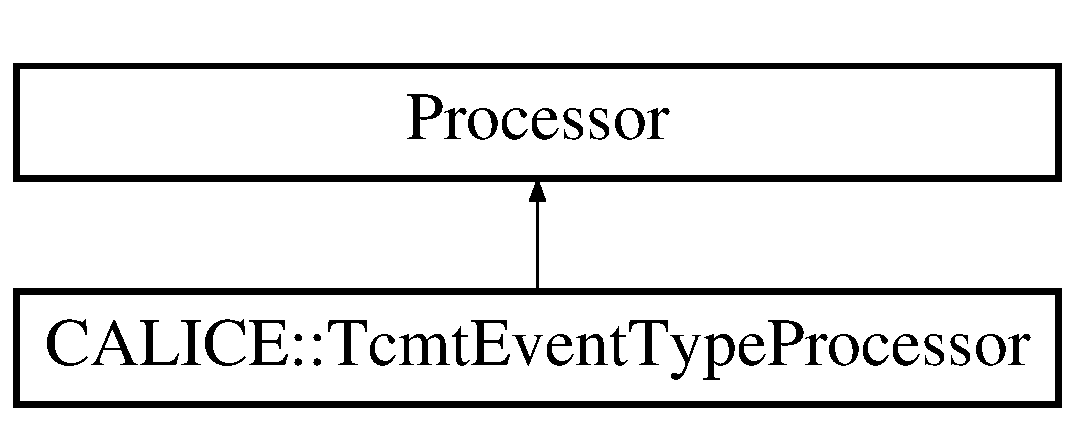
\includegraphics[height=2.000000cm]{classCALICE_1_1TcmtEventTypeProcessor}
\end{center}
\end{figure}
\subsection*{Public Member Functions}
\begin{DoxyCompactItemize}
\item 
virtual Processor $\ast$ {\bfseries new\-Processor} ()\label{classCALICE_1_1TcmtEventTypeProcessor_a3bf9b0177f015c026cdaa89bdce6f597}

\item 
virtual void {\bfseries init} ()\label{classCALICE_1_1TcmtEventTypeProcessor_abc438f27b158fbaa33c64b9143396db1}

\item 
virtual void {\bfseries process\-Event} (L\-C\-Event $\ast$evt)\label{classCALICE_1_1TcmtEventTypeProcessor_a550cdda1709621ee6818c0039284f533}

\item 
virtual void {\bfseries end} ()\label{classCALICE_1_1TcmtEventTypeProcessor_abfc2f5366a03cc51aaab06eed36e28e9}

\end{DoxyCompactItemize}


\subsection{Detailed Description}
Processor that analyses the T\-C\-M\-T event data and returns a bit reflecting the result

\begin{DoxyParagraph}{processor parameters}
\begin{TabularC}{2}
\hline
steering file parameter name &description  \\\cline{1-2}
{\bfseries {\itshape  Input\-Collection }}&name of the input collection  \\\cline{1-2}
{\bfseries {\itshape  Tcmt\-Event\-Bit\-Name }}&name of event parameter that will contain the output bits \\\cline{1-2}
{\bfseries {\itshape  Overwrite\-Encoding }}&encoding string used instead of encoding string of collection (optional)  \\\cline{1-2}
\end{TabularC}

\end{DoxyParagraph}
\begin{DoxyAuthor}{Author}
{\tt Benjamin.\-Lutz@desy.\-de} 
\end{DoxyAuthor}
\begin{DoxyVersion}{Version}
1.\-0 
\end{DoxyVersion}
\begin{DoxyDate}{Date}
November 2009 
\end{DoxyDate}


The documentation for this class was generated from the following files\-:\begin{DoxyCompactItemize}
\item 
/nfs/dust/ilc/user/marquezh/\-Calice\-Soft\-\_\-w\-\_\-\-I\-L\-C\-Soft\-\_\-v02-\/03-\/02/calice\-\_\-analysis/addon\-Procs/include/Tcmt\-Event\-Type\-Processor.\-hh\item 
/nfs/dust/ilc/user/marquezh/\-Calice\-Soft\-\_\-w\-\_\-\-I\-L\-C\-Soft\-\_\-v02-\/03-\/02/calice\-\_\-analysis/addon\-Procs/src/Tcmt\-Event\-Type\-Processor.\-cc\end{DoxyCompactItemize}

\section{C\-A\-L\-I\-C\-E\-:\-:Tcmt\-Muon\-Tracker Class Reference}
\label{classCALICE_1_1TcmtMuonTracker}\index{C\-A\-L\-I\-C\-E\-::\-Tcmt\-Muon\-Tracker@{C\-A\-L\-I\-C\-E\-::\-Tcmt\-Muon\-Tracker}}


{\ttfamily \#include $<$Tcmt\-Muon\-Tracker.\-hh$>$}

Inheritance diagram for C\-A\-L\-I\-C\-E\-:\-:Tcmt\-Muon\-Tracker\-:\begin{figure}[H]
\begin{center}
\leavevmode
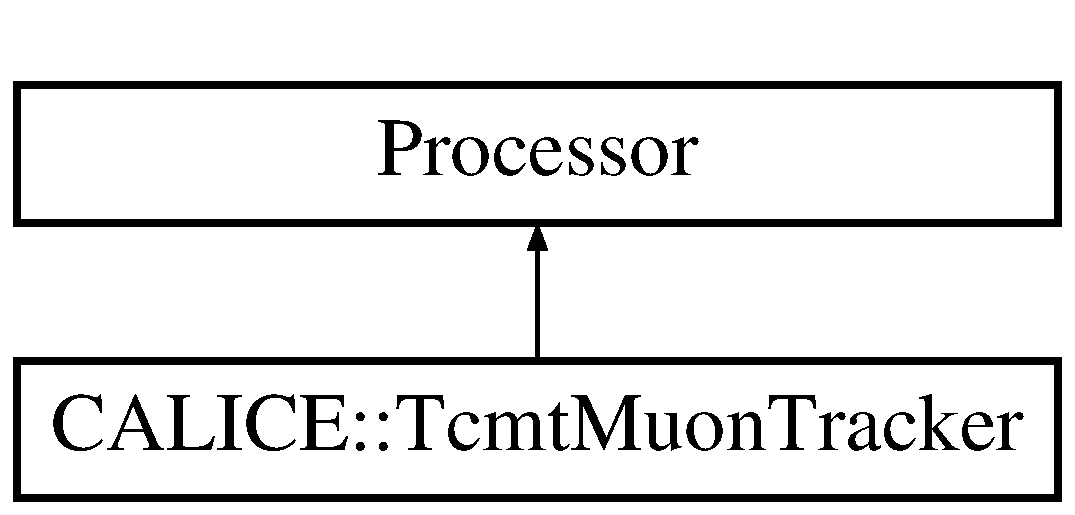
\includegraphics[height=2.000000cm]{classCALICE_1_1TcmtMuonTracker}
\end{center}
\end{figure}
\subsection*{Classes}
\begin{DoxyCompactItemize}
\item 
struct {\bf tcmt\-Tower}
\end{DoxyCompactItemize}
\subsection*{Public Member Functions}
\begin{DoxyCompactItemize}
\item 
Processor $\ast$ {\bfseries new\-Processor} ()\label{classCALICE_1_1TcmtMuonTracker_a128370dc29c7099de47c9735047ffb35}

\item 
void {\bf init} ()
\item 
void {\bf process\-Run\-Header} (L\-C\-Run\-Header $\ast$run)
\item 
void {\bf process\-Event} (L\-C\-Event $\ast$evt)
\item 
void {\bfseries end} ()\label{classCALICE_1_1TcmtMuonTracker_aaa57745b64b3b04cc6b45a5a3dc1f19e}

\end{DoxyCompactItemize}
\subsection*{Protected Member Functions}
\begin{DoxyCompactItemize}
\item 
unsigned {\bf get\-Tower\-I\-Dfrom\-I\-J} (unsigned i\-\_\-pos, unsigned j\-\_\-pos)
\item 
unsigned {\bf get\-Jfrom\-Tower\-I\-D} (unsigned tower\-I\-D)
\item 
unsigned {\bf get\-Ifrom\-Tower\-I\-D} (unsigned tower\-I\-D)
\item 
void {\bf find2\-D\-Towers} (std\-::map$<$ unsigned, Calorimeter\-Hit $\ast$ $>$, Decoder\-Set $\ast$, std\-::list$<$ unsigned $>$, std\-::list$<$ unsigned $>$, std\-::map$<$ unsigned, {\bf tcmt\-Tower} $>$ \&)
\item 
void {\bf merge2\-D\-Towers} (std\-::map$<$ unsigned, {\bf tcmt\-Tower} $>$ \&, std\-::map$<$ unsigned, {\bf tcmt\-Tower} $>$ \&)
\item 
void {\bf find\-Neighbours} ({\bf tcmt\-Tower} \&, std\-::map$<$ unsigned, {\bf tcmt\-Tower} $>$ \&)
\item 
void {\bf fill\-Output\-Collection} (L\-C\-Event $\ast$evt, {\bf tcmt\-Tower} \&muon\-Tower, L\-C\-Collection $\ast$input\-Col, std\-::map$<$ unsigned, Calorimeter\-Hit $\ast$ $>$ hit\-Map\-\_\-all, Decoder\-Set $\ast$decoder)
\end{DoxyCompactItemize}
\subsection*{Protected Attributes}
\begin{DoxyCompactItemize}
\item 
std\-::string {\bf \-\_\-tcm\-Hit\-Col\-Name}
\item 
float {\bf \-\_\-mip\-Threshold}
\item 
int {\bf \-\_\-k\-Threshold}
\item 
Int\-Vec {\bf \-\_\-mu\-\_\-n\-Hits\-\_\-isolated}
\item 
Float\-Vec {\bf \-\_\-mu\-\_\-e\-Sum\-\_\-isolated}
\item 
std\-::string {\bf \-\_\-output\-Col\-Name}
\item 
bool {\bf \-\_\-tcmt\-Start\-Vertical}
\item 
struct \\*
{\bf C\-A\-L\-I\-C\-E\-::\-Tcmt\-Muon\-Tracker\-::tcmt\-Tower} {\bfseries \-\_\-new\-Tower}\label{classCALICE_1_1TcmtMuonTracker_a8189d19eeacdfabf3c5d71c97962f743}

\end{DoxyCompactItemize}
\subsection*{Static Protected Attributes}
\begin{DoxyCompactItemize}
\item 
static const unsigned int {\bfseries M\-A\-X\-\_\-\-T\-C\-M\-T\-\_\-\-L\-A\-Y\-E\-R\-S} = 16\label{classCALICE_1_1TcmtMuonTracker_a34a47144d814ad6080e2ae513f53be68}

\end{DoxyCompactItemize}


\subsection{Detailed Description}
Processor which identifies muons in the T\-C\-M\-T by creating 2\-D (i-\/j) towers from hits in horizontal and vertical strips.

The tower dimension is defined by the overlap betwen T\-C\-M\-T strips with different orientation (5cm x 5 cm).

If the number of hits and the energy sum in the largest tower are above the corresponding thresholds, the event is flagged as containing a muon by setting an event parameter.

The maximum tower is the tower with the largest number of hits (largest visible energy if tie).

The processor appends the following event parameters for the maximum tower found to each event\-:

Processor\-Name\-\_\-max\-Tower\-\_\-e\-Sum -\/$>$ total visible energy from all hits in this tower Processor\-Name\-\_\-max\-Tower\-\_\-n\-Hits -\/$>$ all hits in this tower Processor\-Name\-\_\-max\-Tower\-\_\-x -\/$>$ x-\/position of tower center Processor\-Name\-\_\-max\-Tower\-\_\-y -\/$>$ y-\/position of tower center Processor\-Name\-\_\-max\-Tower\-\_\-track\-I\-D\-\_\-e\-Sum -\/$>$ total visible energy from all hits in this tower that are N\-O\-T I\-S\-O\-L\-A\-T\-E\-D in z Processor\-Name\-\_\-max\-Tower\-\_\-track\-I\-D\-\_\-n\-Hits -\/$>$ all hits in this tower that are N\-O\-T I\-S\-O\-L\-A\-T\-E\-D in z Processor\-Name\-\_\-max\-Tower\-\_\-n\-Neighbours -\/$>$ number of neighboring towers Processor\-Name\-\_\-max\-Tower\-\_\-col\-\_\-e\-Sum -\/$>$ total visible energy from all hits in this tower + neighboring towers Processor\-Name\-\_\-max\-Tower\-\_\-col\-\_\-n\-Hits -\/$>$ all hits in this tower + neighboring towers

\begin{DoxyAuthor}{Author}
{\tt nils.\-feege@desy.\-de} 
\end{DoxyAuthor}
\begin{DoxyDate}{Date}
Oct 2010 
\end{DoxyDate}


\subsection{Member Function Documentation}
\index{C\-A\-L\-I\-C\-E\-::\-Tcmt\-Muon\-Tracker@{C\-A\-L\-I\-C\-E\-::\-Tcmt\-Muon\-Tracker}!fill\-Output\-Collection@{fill\-Output\-Collection}}
\index{fill\-Output\-Collection@{fill\-Output\-Collection}!CALICE::TcmtMuonTracker@{C\-A\-L\-I\-C\-E\-::\-Tcmt\-Muon\-Tracker}}
\subsubsection[{fill\-Output\-Collection}]{\setlength{\rightskip}{0pt plus 5cm}void C\-A\-L\-I\-C\-E\-::\-Tcmt\-Muon\-Tracker\-::fill\-Output\-Collection (
\begin{DoxyParamCaption}
\item[{L\-C\-Event $\ast$}]{evt, }
\item[{{\bf tcmt\-Tower} \&}]{muon\-Tower, }
\item[{L\-C\-Collection $\ast$}]{input\-Col, }
\item[{std\-::map$<$ unsigned, Calorimeter\-Hit $\ast$ $>$}]{hit\-Map\-\_\-all, }
\item[{Decoder\-Set $\ast$}]{decoder}
\end{DoxyParamCaption}
)\hspace{0.3cm}{\ttfamily [protected]}}\label{classCALICE_1_1TcmtMuonTracker_ad70afc55b26be73d3b660573dc8c4c83}
Fill output collection with the hits which belong to the muon tower \index{C\-A\-L\-I\-C\-E\-::\-Tcmt\-Muon\-Tracker@{C\-A\-L\-I\-C\-E\-::\-Tcmt\-Muon\-Tracker}!find2\-D\-Towers@{find2\-D\-Towers}}
\index{find2\-D\-Towers@{find2\-D\-Towers}!CALICE::TcmtMuonTracker@{C\-A\-L\-I\-C\-E\-::\-Tcmt\-Muon\-Tracker}}
\subsubsection[{find2\-D\-Towers}]{\setlength{\rightskip}{0pt plus 5cm}void C\-A\-L\-I\-C\-E\-::\-Tcmt\-Muon\-Tracker\-::find2\-D\-Towers (
\begin{DoxyParamCaption}
\item[{std\-::map$<$ unsigned, Calorimeter\-Hit $\ast$ $>$}]{hit\-Map\-\_\-all, }
\item[{Decoder\-Set $\ast$}]{decoder, }
\item[{std\-::list$<$ unsigned $>$}]{list\-\_\-i\-\_\-hit, }
\item[{std\-::list$<$ unsigned $>$}]{list\-\_\-j\-\_\-hit, }
\item[{std\-::map$<$ unsigned, {\bf tcmt\-Tower} $>$ \&}]{tcmt\-Tower\-Map\-\_\-2d}
\end{DoxyParamCaption}
)\hspace{0.3cm}{\ttfamily [protected]}}\label{classCALICE_1_1TcmtMuonTracker_af16d5d3f4077325b78f35127585ebe3e}
Function filling the tower map by looking for crosses in consecutive layers; the orientation of the first hit layer is not relevant \index{C\-A\-L\-I\-C\-E\-::\-Tcmt\-Muon\-Tracker@{C\-A\-L\-I\-C\-E\-::\-Tcmt\-Muon\-Tracker}!find\-Neighbours@{find\-Neighbours}}
\index{find\-Neighbours@{find\-Neighbours}!CALICE::TcmtMuonTracker@{C\-A\-L\-I\-C\-E\-::\-Tcmt\-Muon\-Tracker}}
\subsubsection[{find\-Neighbours}]{\setlength{\rightskip}{0pt plus 5cm}void C\-A\-L\-I\-C\-E\-::\-Tcmt\-Muon\-Tracker\-::find\-Neighbours (
\begin{DoxyParamCaption}
\item[{{\bf tcmt\-Tower} \&}]{tcmt\-Tower\-X, }
\item[{std\-::map$<$ unsigned, {\bf tcmt\-Tower} $>$ \&}]{tcmt\-Tower\-Map\-\_\-2d}
\end{DoxyParamCaption}
)\hspace{0.3cm}{\ttfamily [protected]}}\label{classCALICE_1_1TcmtMuonTracker_a23b5797a238d16f51bdfaa7c9926fa5b}
function adding neighbour information to singel tower \index{C\-A\-L\-I\-C\-E\-::\-Tcmt\-Muon\-Tracker@{C\-A\-L\-I\-C\-E\-::\-Tcmt\-Muon\-Tracker}!get\-Ifrom\-Tower\-I\-D@{get\-Ifrom\-Tower\-I\-D}}
\index{get\-Ifrom\-Tower\-I\-D@{get\-Ifrom\-Tower\-I\-D}!CALICE::TcmtMuonTracker@{C\-A\-L\-I\-C\-E\-::\-Tcmt\-Muon\-Tracker}}
\subsubsection[{get\-Ifrom\-Tower\-I\-D}]{\setlength{\rightskip}{0pt plus 5cm}unsigned C\-A\-L\-I\-C\-E\-::\-Tcmt\-Muon\-Tracker\-::get\-Ifrom\-Tower\-I\-D (
\begin{DoxyParamCaption}
\item[{unsigned}]{tower\-I\-D}
\end{DoxyParamCaption}
)\hspace{0.3cm}{\ttfamily [inline]}, {\ttfamily [protected]}}\label{classCALICE_1_1TcmtMuonTracker_a35cf4df2bde3a100465b4f6b72c6d56f}
get I from tower I\-D 

References get\-Jfrom\-Tower\-I\-D().

\index{C\-A\-L\-I\-C\-E\-::\-Tcmt\-Muon\-Tracker@{C\-A\-L\-I\-C\-E\-::\-Tcmt\-Muon\-Tracker}!get\-Jfrom\-Tower\-I\-D@{get\-Jfrom\-Tower\-I\-D}}
\index{get\-Jfrom\-Tower\-I\-D@{get\-Jfrom\-Tower\-I\-D}!CALICE::TcmtMuonTracker@{C\-A\-L\-I\-C\-E\-::\-Tcmt\-Muon\-Tracker}}
\subsubsection[{get\-Jfrom\-Tower\-I\-D}]{\setlength{\rightskip}{0pt plus 5cm}unsigned C\-A\-L\-I\-C\-E\-::\-Tcmt\-Muon\-Tracker\-::get\-Jfrom\-Tower\-I\-D (
\begin{DoxyParamCaption}
\item[{unsigned}]{tower\-I\-D}
\end{DoxyParamCaption}
)\hspace{0.3cm}{\ttfamily [inline]}, {\ttfamily [protected]}}\label{classCALICE_1_1TcmtMuonTracker_aa7db26392be38e84f2d9541dfacd42b1}
get J from tower I\-D 

Referenced by get\-Ifrom\-Tower\-I\-D().

\index{C\-A\-L\-I\-C\-E\-::\-Tcmt\-Muon\-Tracker@{C\-A\-L\-I\-C\-E\-::\-Tcmt\-Muon\-Tracker}!get\-Tower\-I\-Dfrom\-I\-J@{get\-Tower\-I\-Dfrom\-I\-J}}
\index{get\-Tower\-I\-Dfrom\-I\-J@{get\-Tower\-I\-Dfrom\-I\-J}!CALICE::TcmtMuonTracker@{C\-A\-L\-I\-C\-E\-::\-Tcmt\-Muon\-Tracker}}
\subsubsection[{get\-Tower\-I\-Dfrom\-I\-J}]{\setlength{\rightskip}{0pt plus 5cm}unsigned C\-A\-L\-I\-C\-E\-::\-Tcmt\-Muon\-Tracker\-::get\-Tower\-I\-Dfrom\-I\-J (
\begin{DoxyParamCaption}
\item[{unsigned}]{i\-\_\-pos, }
\item[{unsigned}]{j\-\_\-pos}
\end{DoxyParamCaption}
)\hspace{0.3cm}{\ttfamily [inline]}, {\ttfamily [protected]}}\label{classCALICE_1_1TcmtMuonTracker_aeed796aa13f75ad5b33d2dd2761b2852}
define I\-D for tower \index{C\-A\-L\-I\-C\-E\-::\-Tcmt\-Muon\-Tracker@{C\-A\-L\-I\-C\-E\-::\-Tcmt\-Muon\-Tracker}!init@{init}}
\index{init@{init}!CALICE::TcmtMuonTracker@{C\-A\-L\-I\-C\-E\-::\-Tcmt\-Muon\-Tracker}}
\subsubsection[{init}]{\setlength{\rightskip}{0pt plus 5cm}void C\-A\-L\-I\-C\-E\-::\-Tcmt\-Muon\-Tracker\-::init (
\begin{DoxyParamCaption}
{}
\end{DoxyParamCaption}
)}\label{classCALICE_1_1TcmtMuonTracker_a7b0e8586bcf666299ec145aecb078b70}
Called at the begin of the job before anything is read. Use to initialize the processor, e.\-g. book histograms. \index{C\-A\-L\-I\-C\-E\-::\-Tcmt\-Muon\-Tracker@{C\-A\-L\-I\-C\-E\-::\-Tcmt\-Muon\-Tracker}!merge2\-D\-Towers@{merge2\-D\-Towers}}
\index{merge2\-D\-Towers@{merge2\-D\-Towers}!CALICE::TcmtMuonTracker@{C\-A\-L\-I\-C\-E\-::\-Tcmt\-Muon\-Tracker}}
\subsubsection[{merge2\-D\-Towers}]{\setlength{\rightskip}{0pt plus 5cm}void C\-A\-L\-I\-C\-E\-::\-Tcmt\-Muon\-Tracker\-::merge2\-D\-Towers (
\begin{DoxyParamCaption}
\item[{std\-::map$<$ unsigned, {\bf tcmt\-Tower} $>$ \&}]{tcmt\-Tower\-Map\-\_\-2d, }
\item[{std\-::map$<$ unsigned, {\bf tcmt\-Tower} $>$ \&}]{tcmt\-Tower\-Map\-\_\-2d\-\_\-merged}
\end{DoxyParamCaption}
)\hspace{0.3cm}{\ttfamily [protected]}}\label{classCALICE_1_1TcmtMuonTracker_a20ce14b6882ffc17e5dcdd4888fbb100}
Function filling the tower map by looking for crosses in consecutive layers, i.\-e. 'hits' in 'superlayers', first hit of cross must be in odd layer, second hit in the next layer\-Function merging towers \index{C\-A\-L\-I\-C\-E\-::\-Tcmt\-Muon\-Tracker@{C\-A\-L\-I\-C\-E\-::\-Tcmt\-Muon\-Tracker}!process\-Event@{process\-Event}}
\index{process\-Event@{process\-Event}!CALICE::TcmtMuonTracker@{C\-A\-L\-I\-C\-E\-::\-Tcmt\-Muon\-Tracker}}
\subsubsection[{process\-Event}]{\setlength{\rightskip}{0pt plus 5cm}void C\-A\-L\-I\-C\-E\-::\-Tcmt\-Muon\-Tracker\-::process\-Event (
\begin{DoxyParamCaption}
\item[{L\-C\-Event $\ast$}]{evt}
\end{DoxyParamCaption}
)}\label{classCALICE_1_1TcmtMuonTracker_a1905c8d9e0d0487708a9266ed59cd344}
Called for every event -\/ this is where the actual action is taking place. \index{C\-A\-L\-I\-C\-E\-::\-Tcmt\-Muon\-Tracker@{C\-A\-L\-I\-C\-E\-::\-Tcmt\-Muon\-Tracker}!process\-Run\-Header@{process\-Run\-Header}}
\index{process\-Run\-Header@{process\-Run\-Header}!CALICE::TcmtMuonTracker@{C\-A\-L\-I\-C\-E\-::\-Tcmt\-Muon\-Tracker}}
\subsubsection[{process\-Run\-Header}]{\setlength{\rightskip}{0pt plus 5cm}void C\-A\-L\-I\-C\-E\-::\-Tcmt\-Muon\-Tracker\-::process\-Run\-Header (
\begin{DoxyParamCaption}
\item[{L\-C\-Run\-Header $\ast$}]{run}
\end{DoxyParamCaption}
)\hspace{0.3cm}{\ttfamily [inline]}}\label{classCALICE_1_1TcmtMuonTracker_a9f5028cbc53811de57bfcc30a4930017}
Called for every run, e.\-g. overwrite to initialize run dependent histograms. 

\subsection{Member Data Documentation}
\index{C\-A\-L\-I\-C\-E\-::\-Tcmt\-Muon\-Tracker@{C\-A\-L\-I\-C\-E\-::\-Tcmt\-Muon\-Tracker}!\-\_\-k\-Threshold@{\-\_\-k\-Threshold}}
\index{\-\_\-k\-Threshold@{\-\_\-k\-Threshold}!CALICE::TcmtMuonTracker@{C\-A\-L\-I\-C\-E\-::\-Tcmt\-Muon\-Tracker}}
\subsubsection[{\-\_\-k\-Threshold}]{\setlength{\rightskip}{0pt plus 5cm}int C\-A\-L\-I\-C\-E\-::\-Tcmt\-Muon\-Tracker\-::\-\_\-k\-Threshold\hspace{0.3cm}{\ttfamily [protected]}}\label{classCALICE_1_1TcmtMuonTracker_a176565b6b2c7632a5485e94d8046a431}
last layer taken into account (counting from 1 to 16) \index{C\-A\-L\-I\-C\-E\-::\-Tcmt\-Muon\-Tracker@{C\-A\-L\-I\-C\-E\-::\-Tcmt\-Muon\-Tracker}!\-\_\-mip\-Threshold@{\-\_\-mip\-Threshold}}
\index{\-\_\-mip\-Threshold@{\-\_\-mip\-Threshold}!CALICE::TcmtMuonTracker@{C\-A\-L\-I\-C\-E\-::\-Tcmt\-Muon\-Tracker}}
\subsubsection[{\-\_\-mip\-Threshold}]{\setlength{\rightskip}{0pt plus 5cm}float C\-A\-L\-I\-C\-E\-::\-Tcmt\-Muon\-Tracker\-::\-\_\-mip\-Threshold\hspace{0.3cm}{\ttfamily [protected]}}\label{classCALICE_1_1TcmtMuonTracker_accede7a68a87dfec941cf6cb430114d9}
Hits with energies below this threshold are ignored \index{C\-A\-L\-I\-C\-E\-::\-Tcmt\-Muon\-Tracker@{C\-A\-L\-I\-C\-E\-::\-Tcmt\-Muon\-Tracker}!\-\_\-mu\-\_\-e\-Sum\-\_\-isolated@{\-\_\-mu\-\_\-e\-Sum\-\_\-isolated}}
\index{\-\_\-mu\-\_\-e\-Sum\-\_\-isolated@{\-\_\-mu\-\_\-e\-Sum\-\_\-isolated}!CALICE::TcmtMuonTracker@{C\-A\-L\-I\-C\-E\-::\-Tcmt\-Muon\-Tracker}}
\subsubsection[{\-\_\-mu\-\_\-e\-Sum\-\_\-isolated}]{\setlength{\rightskip}{0pt plus 5cm}Float\-Vec C\-A\-L\-I\-C\-E\-::\-Tcmt\-Muon\-Tracker\-::\-\_\-mu\-\_\-e\-Sum\-\_\-isolated\hspace{0.3cm}{\ttfamily [protected]}}\label{classCALICE_1_1TcmtMuonTracker_a8c34b0122050e01951c9ae2cba8564dd}
The minimum energy sum (isolated hits) required for a tower (combined horizontal and vertical strips) for identifying a muon in the event \index{C\-A\-L\-I\-C\-E\-::\-Tcmt\-Muon\-Tracker@{C\-A\-L\-I\-C\-E\-::\-Tcmt\-Muon\-Tracker}!\-\_\-mu\-\_\-n\-Hits\-\_\-isolated@{\-\_\-mu\-\_\-n\-Hits\-\_\-isolated}}
\index{\-\_\-mu\-\_\-n\-Hits\-\_\-isolated@{\-\_\-mu\-\_\-n\-Hits\-\_\-isolated}!CALICE::TcmtMuonTracker@{C\-A\-L\-I\-C\-E\-::\-Tcmt\-Muon\-Tracker}}
\subsubsection[{\-\_\-mu\-\_\-n\-Hits\-\_\-isolated}]{\setlength{\rightskip}{0pt plus 5cm}Int\-Vec C\-A\-L\-I\-C\-E\-::\-Tcmt\-Muon\-Tracker\-::\-\_\-mu\-\_\-n\-Hits\-\_\-isolated\hspace{0.3cm}{\ttfamily [protected]}}\label{classCALICE_1_1TcmtMuonTracker_afffea757fd234d2d55bb2c1cf23ae53b}
The minimum number of isolated hits required for a tower (combined horizontal and vertical strips) for identifying a muon in the event \index{C\-A\-L\-I\-C\-E\-::\-Tcmt\-Muon\-Tracker@{C\-A\-L\-I\-C\-E\-::\-Tcmt\-Muon\-Tracker}!\-\_\-output\-Col\-Name@{\-\_\-output\-Col\-Name}}
\index{\-\_\-output\-Col\-Name@{\-\_\-output\-Col\-Name}!CALICE::TcmtMuonTracker@{C\-A\-L\-I\-C\-E\-::\-Tcmt\-Muon\-Tracker}}
\subsubsection[{\-\_\-output\-Col\-Name}]{\setlength{\rightskip}{0pt plus 5cm}std\-::string C\-A\-L\-I\-C\-E\-::\-Tcmt\-Muon\-Tracker\-::\-\_\-output\-Col\-Name\hspace{0.3cm}{\ttfamily [protected]}}\label{classCALICE_1_1TcmtMuonTracker_acd5664e441ae2efdd05146f5bc084e18}
The name of the output collection (which contains the hits belonging to the muon track) \index{C\-A\-L\-I\-C\-E\-::\-Tcmt\-Muon\-Tracker@{C\-A\-L\-I\-C\-E\-::\-Tcmt\-Muon\-Tracker}!\-\_\-tcm\-Hit\-Col\-Name@{\-\_\-tcm\-Hit\-Col\-Name}}
\index{\-\_\-tcm\-Hit\-Col\-Name@{\-\_\-tcm\-Hit\-Col\-Name}!CALICE::TcmtMuonTracker@{C\-A\-L\-I\-C\-E\-::\-Tcmt\-Muon\-Tracker}}
\subsubsection[{\-\_\-tcm\-Hit\-Col\-Name}]{\setlength{\rightskip}{0pt plus 5cm}std\-::string C\-A\-L\-I\-C\-E\-::\-Tcmt\-Muon\-Tracker\-::\-\_\-tcm\-Hit\-Col\-Name\hspace{0.3cm}{\ttfamily [protected]}}\label{classCALICE_1_1TcmtMuonTracker_a38b35b31703cb74d4a43a10eb80324cc}
The name of the T\-C\-M\-T hit input collection \index{C\-A\-L\-I\-C\-E\-::\-Tcmt\-Muon\-Tracker@{C\-A\-L\-I\-C\-E\-::\-Tcmt\-Muon\-Tracker}!\-\_\-tcmt\-Start\-Vertical@{\-\_\-tcmt\-Start\-Vertical}}
\index{\-\_\-tcmt\-Start\-Vertical@{\-\_\-tcmt\-Start\-Vertical}!CALICE::TcmtMuonTracker@{C\-A\-L\-I\-C\-E\-::\-Tcmt\-Muon\-Tracker}}
\subsubsection[{\-\_\-tcmt\-Start\-Vertical}]{\setlength{\rightskip}{0pt plus 5cm}bool C\-A\-L\-I\-C\-E\-::\-Tcmt\-Muon\-Tracker\-::\-\_\-tcmt\-Start\-Vertical\hspace{0.3cm}{\ttfamily [protected]}}\label{classCALICE_1_1TcmtMuonTracker_aaf9afbe718fe44833b890a1e522c3b87}
Flag to set the orientation of the first T\-C\-M\-T layer (1=vertical, 0=horizontal) 

The documentation for this class was generated from the following files\-:\begin{DoxyCompactItemize}
\item 
/nfs/dust/ilc/user/marquezh/\-Calice\-Soft\-\_\-w\-\_\-\-I\-L\-C\-Soft\-\_\-v02-\/03-\/02/calice\-\_\-analysis/addon\-Procs/include/Tcmt\-Muon\-Tracker.\-hh\item 
/nfs/dust/ilc/user/marquezh/\-Calice\-Soft\-\_\-w\-\_\-\-I\-L\-C\-Soft\-\_\-v02-\/03-\/02/calice\-\_\-analysis/addon\-Procs/src/Tcmt\-Muon\-Tracker.\-cc\end{DoxyCompactItemize}

\section{C\-A\-L\-I\-C\-E\-:\-:Tcmt\-Muon\-Tracker\-:\-:tcmt\-Tower Struct Reference}
\label{structCALICE_1_1TcmtMuonTracker_1_1tcmtTower}\index{C\-A\-L\-I\-C\-E\-::\-Tcmt\-Muon\-Tracker\-::tcmt\-Tower@{C\-A\-L\-I\-C\-E\-::\-Tcmt\-Muon\-Tracker\-::tcmt\-Tower}}


{\ttfamily \#include $<$Tcmt\-Muon\-Tracker.\-hh$>$}

\subsection*{Public Attributes}
\begin{DoxyCompactItemize}
\item 
unsigned {\bfseries i}\label{structCALICE_1_1TcmtMuonTracker_1_1tcmtTower_a81331a658a56eff9d47a9fc0ec9fd9a7}

\item 
unsigned {\bfseries j}\label{structCALICE_1_1TcmtMuonTracker_1_1tcmtTower_aba757f07daad80a7403e5d1e7a55ff6b}

\item 
float {\bfseries e\-Sum}\label{structCALICE_1_1TcmtMuonTracker_1_1tcmtTower_a7cf2bbaeab8749bdb5286dfc7deb2d82}

\item 
float {\bfseries e\-Sum\-\_\-front}\label{structCALICE_1_1TcmtMuonTracker_1_1tcmtTower_a20ffe699f59b5d2b46ad843baaf7cbd7}

\item 
float {\bfseries e\-Sum\-\_\-back}\label{structCALICE_1_1TcmtMuonTracker_1_1tcmtTower_ae2fceb827ddacce2cce32ca81e157115}

\item 
int {\bfseries n\-Hits}\label{structCALICE_1_1TcmtMuonTracker_1_1tcmtTower_aed4e14d0f188329b849d064e980b294a}

\item 
int {\bfseries n\-Hits\-\_\-front}\label{structCALICE_1_1TcmtMuonTracker_1_1tcmtTower_a95f9154793306f4abc35d6bee1e7dc85}

\item 
int {\bfseries n\-Hits\-\_\-back}\label{structCALICE_1_1TcmtMuonTracker_1_1tcmtTower_a025318fe5b7eea301e55fae0d63708de}

\item 
float {\bfseries xstart}\label{structCALICE_1_1TcmtMuonTracker_1_1tcmtTower_a5b04ba3b9ce5de1c95c3b56ed297709c}

\item 
float {\bfseries xend}\label{structCALICE_1_1TcmtMuonTracker_1_1tcmtTower_a40c1091d45eda4386e4c9057ae154db7}

\item 
float {\bfseries ystart}\label{structCALICE_1_1TcmtMuonTracker_1_1tcmtTower_a9cd6f3e15e8cd21480a218bb35d3dc89}

\item 
float {\bfseries yend}\label{structCALICE_1_1TcmtMuonTracker_1_1tcmtTower_aa60be9a496a38bd17d276e2c174bc7dc}

\item 
float {\bfseries zstart}\label{structCALICE_1_1TcmtMuonTracker_1_1tcmtTower_a3372a0ec966a91ec67b00063c7bdfb33}

\item 
float {\bfseries zend}\label{structCALICE_1_1TcmtMuonTracker_1_1tcmtTower_afaa0810a3d827db4ec6253f37f4c851e}

\item 
int {\bfseries track\-I\-D\-\_\-n\-Hits}\label{structCALICE_1_1TcmtMuonTracker_1_1tcmtTower_ab6c9361c2d0f1f787a149e6291455dbd}

\item 
float {\bfseries track\-I\-D\-\_\-e\-Sum}\label{structCALICE_1_1TcmtMuonTracker_1_1tcmtTower_ab32287988385bb47951c75dadddadd0a}

\item 
int {\bfseries n\-Neighbours}\label{structCALICE_1_1TcmtMuonTracker_1_1tcmtTower_a77047b480e6ed855d633bde5fda4df27}

\item 
int {\bfseries col\-\_\-n\-Hits}\label{structCALICE_1_1TcmtMuonTracker_1_1tcmtTower_a52fa47d9d817a05ee1464f9766261aec}

\item 
float {\bfseries col\-\_\-e\-Sum}\label{structCALICE_1_1TcmtMuonTracker_1_1tcmtTower_ad79c9a17809bdd59bb2adb1a3ce54944}

\end{DoxyCompactItemize}


\subsection{Detailed Description}
structure collecting tower information 

The documentation for this struct was generated from the following file\-:\begin{DoxyCompactItemize}
\item 
/nfs/dust/ilc/user/marquezh/\-Calice\-Soft\-\_\-w\-\_\-\-I\-L\-C\-Soft\-\_\-v02-\/03-\/02/calice\-\_\-analysis/addon\-Procs/include/Tcmt\-Muon\-Tracker.\-hh\end{DoxyCompactItemize}

\section{C\-A\-L\-I\-C\-E\-:\-:Track\-Validation\-Processor Class Reference}
\label{classCALICE_1_1TrackValidationProcessor}\index{C\-A\-L\-I\-C\-E\-::\-Track\-Validation\-Processor@{C\-A\-L\-I\-C\-E\-::\-Track\-Validation\-Processor}}
Inheritance diagram for C\-A\-L\-I\-C\-E\-:\-:Track\-Validation\-Processor\-:\begin{figure}[H]
\begin{center}
\leavevmode
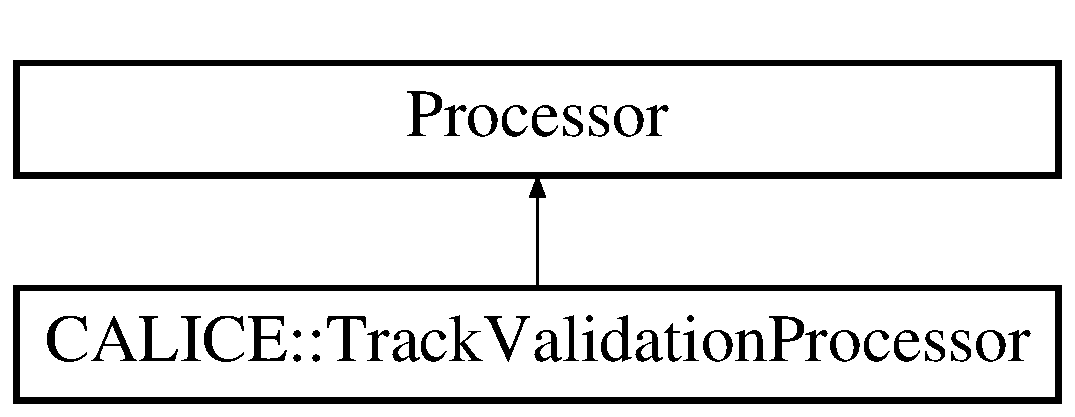
\includegraphics[height=2.000000cm]{classCALICE_1_1TrackValidationProcessor}
\end{center}
\end{figure}
\subsection*{Public Member Functions}
\begin{DoxyCompactItemize}
\item 
virtual Processor $\ast$ {\bfseries new\-Processor} ()\label{classCALICE_1_1TrackValidationProcessor_aab6ced0d983b435a5b9524b6af9b8fab}

\item 
virtual void {\bfseries init} ()\label{classCALICE_1_1TrackValidationProcessor_ab80de3e3a345b87b67499420a6a6e2da}

\item 
virtual void {\bfseries process\-Run\-Header} (L\-C\-Run\-Header $\ast$run)\label{classCALICE_1_1TrackValidationProcessor_a41ff5e507417459b4eacccd9073bce3e}

\item 
virtual void {\bfseries process\-Event} (L\-C\-Event $\ast$evt)\label{classCALICE_1_1TrackValidationProcessor_a3f5d0bcd0d0fb86398db8e25dcaf3884}

\item 
virtual void {\bfseries check} (L\-C\-Event $\ast$evt)\label{classCALICE_1_1TrackValidationProcessor_a45f45ade83bd6f8111fe9794251c963f}

\item 
virtual void {\bfseries end} ()\label{classCALICE_1_1TrackValidationProcessor_a2478d1c6021e9f78a5a7489ecafe61cc}

\item 
virtual void {\bfseries print\-Parameters} ()\label{classCALICE_1_1TrackValidationProcessor_a86b4f58b01d3a5b21cb409b6608cafc7}

\end{DoxyCompactItemize}
\subsection*{Protected Attributes}
\begin{DoxyCompactItemize}
\item 
std\-::string {\bfseries \-\_\-evt\-Var\-Col\-Name}\label{classCALICE_1_1TrackValidationProcessor_a76ddd6b305410b6413f073d741743ee0}

\item 
std\-::string {\bfseries \-\_\-lay\-Var\-Col\-Name}\label{classCALICE_1_1TrackValidationProcessor_a7161ade55449fddbff031a7f6f205c5b}

\item 
std\-::string {\bfseries \-\_\-hit\-In\-Col\-Name}\label{classCALICE_1_1TrackValidationProcessor_aa37bb1a3f8daad8869a739424424b1a4}

\item 
std\-::string {\bfseries \-\_\-\-M\-C\-Particle\-Col\-Name}\label{classCALICE_1_1TrackValidationProcessor_a7cb2eb63f3742d45bcb200ab856ee369}

\item 
std\-::string {\bfseries \-\_\-\-D\-W\-C\-Col\-Name}\label{classCALICE_1_1TrackValidationProcessor_aa7967db3adedfaf442fbd0c305327fcb}

\item 
float {\bfseries \-\_\-xoffset}\label{classCALICE_1_1TrackValidationProcessor_a0e591b95122cdc9574bc4920b3e0284c}

\item 
float {\bfseries \-\_\-yoffset}\label{classCALICE_1_1TrackValidationProcessor_a4939b52b2b0f0ffafe839d1d3a370cdf}

\item 
int {\bf \-\_\-n\-Run}
\item 
int {\bf \-\_\-n\-Evt}
\item 
std\-::string {\bfseries \-\_\-rootoutput}\label{classCALICE_1_1TrackValidationProcessor_a91381cdf201234a7adc8f0169ab2c97b}

\item 
bool {\bfseries \-\_\-is\-M\-C}\label{classCALICE_1_1TrackValidationProcessor_a42090c30cc0793268a7346b01b7216a2}

\end{DoxyCompactItemize}


\subsection{Member Data Documentation}
\index{C\-A\-L\-I\-C\-E\-::\-Track\-Validation\-Processor@{C\-A\-L\-I\-C\-E\-::\-Track\-Validation\-Processor}!\-\_\-n\-Evt@{\-\_\-n\-Evt}}
\index{\-\_\-n\-Evt@{\-\_\-n\-Evt}!CALICE::TrackValidationProcessor@{C\-A\-L\-I\-C\-E\-::\-Track\-Validation\-Processor}}
\subsubsection[{\-\_\-n\-Evt}]{\setlength{\rightskip}{0pt plus 5cm}int C\-A\-L\-I\-C\-E\-::\-Track\-Validation\-Processor\-::\-\_\-n\-Evt\hspace{0.3cm}{\ttfamily [protected]}}\label{classCALICE_1_1TrackValidationProcessor_aa416b3b756c930a0dea555886d1cf39c}
evt number \index{C\-A\-L\-I\-C\-E\-::\-Track\-Validation\-Processor@{C\-A\-L\-I\-C\-E\-::\-Track\-Validation\-Processor}!\-\_\-n\-Run@{\-\_\-n\-Run}}
\index{\-\_\-n\-Run@{\-\_\-n\-Run}!CALICE::TrackValidationProcessor@{C\-A\-L\-I\-C\-E\-::\-Track\-Validation\-Processor}}
\subsubsection[{\-\_\-n\-Run}]{\setlength{\rightskip}{0pt plus 5cm}int C\-A\-L\-I\-C\-E\-::\-Track\-Validation\-Processor\-::\-\_\-n\-Run\hspace{0.3cm}{\ttfamily [protected]}}\label{classCALICE_1_1TrackValidationProcessor_af235f7e8a5a00894c66e467f55552bfe}
run number 

The documentation for this class was generated from the following files\-:\begin{DoxyCompactItemize}
\item 
/nfs/dust/ilc/user/marquezh/\-Calice\-Soft\-\_\-w\-\_\-\-I\-L\-C\-Soft\-\_\-v02-\/03-\/02/calice\-\_\-analysis/addon\-Procs/include/Track\-Validation.\-hh\item 
/nfs/dust/ilc/user/marquezh/\-Calice\-Soft\-\_\-w\-\_\-\-I\-L\-C\-Soft\-\_\-v02-\/03-\/02/calice\-\_\-analysis/addon\-Procs/src/Track\-Validation.\-cc\end{DoxyCompactItemize}

\section{C\-A\-L\-I\-C\-E\-:\-:Track\-Variables Class Reference}
\label{classCALICE_1_1TrackVariables}\index{C\-A\-L\-I\-C\-E\-::\-Track\-Variables@{C\-A\-L\-I\-C\-E\-::\-Track\-Variables}}
\subsection*{Public Member Functions}
\begin{DoxyCompactItemize}
\item 
{\bf Track\-Variables} ()
\item 
{\bf $\sim$\-Track\-Variables} ()
\end{DoxyCompactItemize}
\subsection*{Public Attributes}
\begin{DoxyCompactItemize}
\item 
int {\bfseries n\-Hits\-\_\-event}\label{classCALICE_1_1TrackVariables_a2a7a84f5ad564c70304acb273129bb3c}

\item 
float {\bfseries cogx\-\_\-event}\label{classCALICE_1_1TrackVariables_af1e98b63ac4bceb890f30c7349ccd9ef}

\item 
float {\bfseries cogy\-\_\-event}\label{classCALICE_1_1TrackVariables_af62f975ce34c4de66c66a16c119bdf7d}

\item 
float {\bfseries cogz\-\_\-event}\label{classCALICE_1_1TrackVariables_a8cee70d5925ef7b1e281c697a9fe196f}

\item 
int {\bfseries n\-Hits\-\_\-layer1}\label{classCALICE_1_1TrackVariables_af24f50d32d6a18d6cc8d858a2db7e5f7}

\item 
float {\bfseries cogx\-\_\-layer1}\label{classCALICE_1_1TrackVariables_a6d2a65b54e9a6c567ea8d4a264a54a2a}

\item 
float {\bfseries cogy\-\_\-layer1}\label{classCALICE_1_1TrackVariables_a7f632529d25ccf4961d127135f6c9d0f}

\item 
float {\bfseries x\-\_\-hit1\-\_\-layer1}\label{classCALICE_1_1TrackVariables_a96384401e1c665deaa1122a3fa6ac56d}

\item 
float {\bfseries x\-\_\-hit2\-\_\-layer1}\label{classCALICE_1_1TrackVariables_aecbf2b238662cefdff6bf14d117573c4}

\item 
float {\bfseries x\-\_\-hit3\-\_\-layer1}\label{classCALICE_1_1TrackVariables_ae61d4a2dc47701014a25f87cb0fdf96a}

\item 
float {\bfseries x\-\_\-hit4\-\_\-layer1}\label{classCALICE_1_1TrackVariables_a0ed5e0ec025f98eabd194dc3021ab88f}

\item 
float {\bfseries x\-\_\-hit5\-\_\-layer1}\label{classCALICE_1_1TrackVariables_af54575bb2c5b7990b63a2f2b909d31f6}

\item 
float {\bfseries x\-\_\-hit6\-\_\-layer1}\label{classCALICE_1_1TrackVariables_a7bdbb745232b0cd60e6163df7029b61d}

\item 
float {\bfseries x\-\_\-hit7\-\_\-layer1}\label{classCALICE_1_1TrackVariables_a052ddb1ee615d793e5a4988c4161392f}

\item 
float {\bfseries x\-\_\-hit8\-\_\-layer1}\label{classCALICE_1_1TrackVariables_ac833ff68a6a61bb5d544290416c59943}

\item 
float {\bfseries x\-\_\-hit9\-\_\-layer1}\label{classCALICE_1_1TrackVariables_afe29e081f05fdbcf88e657ec69022c3e}

\item 
float {\bfseries x\-\_\-hit10\-\_\-layer1}\label{classCALICE_1_1TrackVariables_ac477ac6dca1a57f2a14943a9cb18c232}

\item 
float {\bfseries x\-\_\-hit11\-\_\-layer1}\label{classCALICE_1_1TrackVariables_aaba8b86614764f776e3ca4df81e4aae5}

\item 
float {\bfseries x\-\_\-hit12\-\_\-layer1}\label{classCALICE_1_1TrackVariables_ac8ead41d85c09c902a580c7dad824049}

\item 
float {\bfseries x\-\_\-hit13\-\_\-layer1}\label{classCALICE_1_1TrackVariables_afbf0707fa594012e6c8fd115d0f7abc4}

\item 
float {\bfseries x\-\_\-hit14\-\_\-layer1}\label{classCALICE_1_1TrackVariables_ab1a2e5dbbe02651426cf8509d68f3785}

\item 
float {\bfseries x\-\_\-hit15\-\_\-layer1}\label{classCALICE_1_1TrackVariables_a0231cd13c2bbd5bd446898a7736b7021}

\item 
float {\bfseries y\-\_\-hit1\-\_\-layer1}\label{classCALICE_1_1TrackVariables_a8f79438d74a5d00741e05ec1ef86aa2a}

\item 
float {\bfseries y\-\_\-hit2\-\_\-layer1}\label{classCALICE_1_1TrackVariables_ac03920c335316e2b6503fd463011a6c0}

\item 
float {\bfseries y\-\_\-hit3\-\_\-layer1}\label{classCALICE_1_1TrackVariables_a70970263e8adcf22ea098c4d187a8d4d}

\item 
float {\bfseries y\-\_\-hit4\-\_\-layer1}\label{classCALICE_1_1TrackVariables_a145e02e5a00024f56a0f24e5daacae90}

\item 
float {\bfseries y\-\_\-hit5\-\_\-layer1}\label{classCALICE_1_1TrackVariables_a0268e2a52fa3db2062f8bf667e8ca8e9}

\item 
float {\bfseries y\-\_\-hit6\-\_\-layer1}\label{classCALICE_1_1TrackVariables_a0280cfa33723bcc561d76fed1cae13d2}

\item 
float {\bfseries y\-\_\-hit7\-\_\-layer1}\label{classCALICE_1_1TrackVariables_a262438e822ae2b1d8a44cdfeade7e1e9}

\item 
float {\bfseries y\-\_\-hit8\-\_\-layer1}\label{classCALICE_1_1TrackVariables_a2df4ebfdd4b24afccfeedefdeb89c6b8}

\item 
float {\bfseries y\-\_\-hit9\-\_\-layer1}\label{classCALICE_1_1TrackVariables_a392310a555ae4b43060ae4fd8880ed83}

\item 
float {\bfseries y\-\_\-hit10\-\_\-layer1}\label{classCALICE_1_1TrackVariables_a7f1becf5eae05c14aeadcba4677c2fe3}

\item 
float {\bfseries y\-\_\-hit11\-\_\-layer1}\label{classCALICE_1_1TrackVariables_a29065e54f31d39cd6fab97c3e23b213c}

\item 
float {\bfseries y\-\_\-hit12\-\_\-layer1}\label{classCALICE_1_1TrackVariables_ab08b4d5f195c304857fd67cfd64ff0e7}

\item 
float {\bfseries y\-\_\-hit13\-\_\-layer1}\label{classCALICE_1_1TrackVariables_a2dcb08f9bbcc3cfa205817ed5095f278}

\item 
float {\bfseries y\-\_\-hit14\-\_\-layer1}\label{classCALICE_1_1TrackVariables_a5ef355691c80f290d90efb5c3a0fb03d}

\item 
float {\bfseries y\-\_\-hit15\-\_\-layer1}\label{classCALICE_1_1TrackVariables_a836ecf23405c59324c3ddecafb31d5af}

\item 
float {\bfseries trackx}\label{classCALICE_1_1TrackVariables_a4ff873456f548b31531bde8dedb49e9a}

\item 
float {\bfseries tracky}\label{classCALICE_1_1TrackVariables_a666437d638c1305c9e750d220b72347b}

\item 
float {\bfseries beamgunpositionx}\label{classCALICE_1_1TrackVariables_ace77703a6f8b2f725fbfd338d5521fb4}

\item 
float {\bfseries beamgunpositiony}\label{classCALICE_1_1TrackVariables_a7a2170d2e97f47892d2949b7e9ef15d4}

\item 
float {\bfseries endpointpositionx}\label{classCALICE_1_1TrackVariables_a2bcf536efed39e8ff699a60f65c82c5f}

\item 
float {\bfseries endpointpositiony}\label{classCALICE_1_1TrackVariables_ac4b4166aa11b2c6a94da7fb6730363b2}

\item 
float {\bfseries endpointpositionz}\label{classCALICE_1_1TrackVariables_a09769d7b4aafcbfebffce076a0612bef}

\item 
float {\bfseries energy\-\_\-primary\-\_\-z}\label{classCALICE_1_1TrackVariables_a5f71d624f636f7ac09224ae8a4e5d8b4}

\item 
float {\bfseries energy\-\_\-leading\-\_\-daughter\-\_\-z}\label{classCALICE_1_1TrackVariables_a42a8b8d50697afe5d05474f3de8a1433}

\end{DoxyCompactItemize}


\subsection{Constructor \& Destructor Documentation}
\index{C\-A\-L\-I\-C\-E\-::\-Track\-Variables@{C\-A\-L\-I\-C\-E\-::\-Track\-Variables}!Track\-Variables@{Track\-Variables}}
\index{Track\-Variables@{Track\-Variables}!CALICE::TrackVariables@{C\-A\-L\-I\-C\-E\-::\-Track\-Variables}}
\subsubsection[{Track\-Variables}]{\setlength{\rightskip}{0pt plus 5cm}C\-A\-L\-I\-C\-E\-::\-Track\-Variables\-::\-Track\-Variables (
\begin{DoxyParamCaption}
{}
\end{DoxyParamCaption}
)\hspace{0.3cm}{\ttfamily [inline]}}\label{classCALICE_1_1TrackVariables_a886c446759eaaaf27fa738044ed57244}
Constructor with member initialization \index{C\-A\-L\-I\-C\-E\-::\-Track\-Variables@{C\-A\-L\-I\-C\-E\-::\-Track\-Variables}!$\sim$\-Track\-Variables@{$\sim$\-Track\-Variables}}
\index{$\sim$\-Track\-Variables@{$\sim$\-Track\-Variables}!CALICE::TrackVariables@{C\-A\-L\-I\-C\-E\-::\-Track\-Variables}}
\subsubsection[{$\sim$\-Track\-Variables}]{\setlength{\rightskip}{0pt plus 5cm}C\-A\-L\-I\-C\-E\-::\-Track\-Variables\-::$\sim$\-Track\-Variables (
\begin{DoxyParamCaption}
{}
\end{DoxyParamCaption}
)\hspace{0.3cm}{\ttfamily [inline]}}\label{classCALICE_1_1TrackVariables_acabb2fcaf917d657508520112afa865c}
Default destructor 

The documentation for this class was generated from the following file\-:\begin{DoxyCompactItemize}
\item 
/nfs/dust/ilc/user/marquezh/\-Calice\-Soft\-\_\-w\-\_\-\-I\-L\-C\-Soft\-\_\-v02-\/03-\/02/calice\-\_\-analysis/addon\-Procs/include/Track\-Validation.\-hh\end{DoxyCompactItemize}

\section{C\-A\-L\-I\-C\-E\-:\-:Virtual\-Cells Class Reference}
\label{classCALICE_1_1VirtualCells}\index{C\-A\-L\-I\-C\-E\-::\-Virtual\-Cells@{C\-A\-L\-I\-C\-E\-::\-Virtual\-Cells}}


{\ttfamily \#include $<$Virtual\-Cells.\-hh$>$}

\subsection*{Public Member Functions}
\begin{DoxyCompactItemize}
\item 
{\bf Virtual\-Cells} (const int cell\-I\-D, const float angle)
\item 
int {\bf get\-Cell\-I\-D} () const 
\item 
unsigned int {\bf get\-Number\-Of\-Virtual\-Cells} () const 
\item 
const float $\ast$ {\bf get\-Virtual\-Cell\-Position} (unsigned int i) const 
\item 
void {\bf add\-Cell} (const float x, const float y, const float z)
\item 
void {\bf add\-Cell} (const float $\ast$position)
\item 
float {\bf get\-Angle} () const 
\end{DoxyCompactItemize}
\subsection*{Protected Attributes}
\begin{DoxyCompactItemize}
\item 
const int {\bfseries \-\_\-cell\-I\-D}\label{classCALICE_1_1VirtualCells_afa83be29e6de5c242fc8a90fff8dde5c}

\item 
const float {\bfseries \-\_\-cell\-Angle}\label{classCALICE_1_1VirtualCells_a4c57922d6b47ce4dece4d7bf6657720e}

\item 
std\-::vector$<$ const float $\ast$ $>$ {\bfseries \-\_\-cell\-Positions}\label{classCALICE_1_1VirtualCells_a939247ffe329c15b1a6530fc48407c83}

\end{DoxyCompactItemize}


\subsection{Detailed Description}
container class for virtual sub cells

\begin{DoxyAuthor}{Author}
{\tt Benjamin.\-Lutz@desy.\-de} 
\end{DoxyAuthor}
\begin{DoxyDate}{Date}
July 2009 
\end{DoxyDate}
\begin{DoxyVersion}{Version}
0.\-1 
\end{DoxyVersion}


\subsection{Constructor \& Destructor Documentation}
\index{C\-A\-L\-I\-C\-E\-::\-Virtual\-Cells@{C\-A\-L\-I\-C\-E\-::\-Virtual\-Cells}!Virtual\-Cells@{Virtual\-Cells}}
\index{Virtual\-Cells@{Virtual\-Cells}!CALICE::VirtualCells@{C\-A\-L\-I\-C\-E\-::\-Virtual\-Cells}}
\subsubsection[{Virtual\-Cells}]{\setlength{\rightskip}{0pt plus 5cm}C\-A\-L\-I\-C\-E\-::\-Virtual\-Cells\-::\-Virtual\-Cells (
\begin{DoxyParamCaption}
\item[{const int}]{cell\-I\-D, }
\item[{const float}]{angle}
\end{DoxyParamCaption}
)}\label{classCALICE_1_1VirtualCells_ac3f91d291b715af9b9b0479e98ba63d6}
constructor


\begin{DoxyParams}{Parameters}
{\em cell\-I\-D} & (Mokka) cell I\-D of the mother cell \\
\hline
{\em angle} & angluar orientation of mother cell \\
\hline
\end{DoxyParams}


\subsection{Member Function Documentation}
\index{C\-A\-L\-I\-C\-E\-::\-Virtual\-Cells@{C\-A\-L\-I\-C\-E\-::\-Virtual\-Cells}!add\-Cell@{add\-Cell}}
\index{add\-Cell@{add\-Cell}!CALICE::VirtualCells@{C\-A\-L\-I\-C\-E\-::\-Virtual\-Cells}}
\subsubsection[{add\-Cell}]{\setlength{\rightskip}{0pt plus 5cm}void C\-A\-L\-I\-C\-E\-::\-Virtual\-Cells\-::add\-Cell (
\begin{DoxyParamCaption}
\item[{const float}]{x, }
\item[{const float}]{y, }
\item[{const float}]{z}
\end{DoxyParamCaption}
)}\label{classCALICE_1_1VirtualCells_acf25df7941d5bf93bea069b09cb9146b}
add sub cell


\begin{DoxyParams}[1]{Parameters}
\mbox{\tt in}  & {\em x} & x position of sub-\/cell \\
\hline
\mbox{\tt in}  & {\em y} & y position of sub-\/cell \\
\hline
\mbox{\tt in}  & {\em z} & z position of sub-\/cell \\
\hline
\end{DoxyParams}


Referenced by C\-A\-L\-I\-C\-E\-::\-Virtual\-Cells\-Calculator\-::calculate().

\index{C\-A\-L\-I\-C\-E\-::\-Virtual\-Cells@{C\-A\-L\-I\-C\-E\-::\-Virtual\-Cells}!add\-Cell@{add\-Cell}}
\index{add\-Cell@{add\-Cell}!CALICE::VirtualCells@{C\-A\-L\-I\-C\-E\-::\-Virtual\-Cells}}
\subsubsection[{add\-Cell}]{\setlength{\rightskip}{0pt plus 5cm}void C\-A\-L\-I\-C\-E\-::\-Virtual\-Cells\-::add\-Cell (
\begin{DoxyParamCaption}
\item[{const float $\ast$}]{position}
\end{DoxyParamCaption}
)}\label{classCALICE_1_1VirtualCells_a429c3423e4d7552359ee125f024bbc9d}
add sub cell


\begin{DoxyParams}[1]{Parameters}
\mbox{\tt in}  & {\em position} & array of 3 floats (x,y,z) \\
\hline
\end{DoxyParams}
\index{C\-A\-L\-I\-C\-E\-::\-Virtual\-Cells@{C\-A\-L\-I\-C\-E\-::\-Virtual\-Cells}!get\-Angle@{get\-Angle}}
\index{get\-Angle@{get\-Angle}!CALICE::VirtualCells@{C\-A\-L\-I\-C\-E\-::\-Virtual\-Cells}}
\subsubsection[{get\-Angle}]{\setlength{\rightskip}{0pt plus 5cm}float C\-A\-L\-I\-C\-E\-::\-Virtual\-Cells\-::get\-Angle (
\begin{DoxyParamCaption}
{}
\end{DoxyParamCaption}
) const\hspace{0.3cm}{\ttfamily [inline]}}\label{classCALICE_1_1VirtualCells_a0c766d3bac6161532603da07c78debcd}
get the angle of cells

\begin{DoxyReturn}{Returns}
angle of cells 
\end{DoxyReturn}
\index{C\-A\-L\-I\-C\-E\-::\-Virtual\-Cells@{C\-A\-L\-I\-C\-E\-::\-Virtual\-Cells}!get\-Cell\-I\-D@{get\-Cell\-I\-D}}
\index{get\-Cell\-I\-D@{get\-Cell\-I\-D}!CALICE::VirtualCells@{C\-A\-L\-I\-C\-E\-::\-Virtual\-Cells}}
\subsubsection[{get\-Cell\-I\-D}]{\setlength{\rightskip}{0pt plus 5cm}int C\-A\-L\-I\-C\-E\-::\-Virtual\-Cells\-::get\-Cell\-I\-D (
\begin{DoxyParamCaption}
{}
\end{DoxyParamCaption}
) const\hspace{0.3cm}{\ttfamily [inline]}}\label{classCALICE_1_1VirtualCells_ac0a30f93a9135338f3fba5c5ecbf518c}
get cell\-I\-D of the mother cell

\begin{DoxyReturn}{Returns}
(Mokka) cell I\-D of mother cell 
\end{DoxyReturn}
\index{C\-A\-L\-I\-C\-E\-::\-Virtual\-Cells@{C\-A\-L\-I\-C\-E\-::\-Virtual\-Cells}!get\-Number\-Of\-Virtual\-Cells@{get\-Number\-Of\-Virtual\-Cells}}
\index{get\-Number\-Of\-Virtual\-Cells@{get\-Number\-Of\-Virtual\-Cells}!CALICE::VirtualCells@{C\-A\-L\-I\-C\-E\-::\-Virtual\-Cells}}
\subsubsection[{get\-Number\-Of\-Virtual\-Cells}]{\setlength{\rightskip}{0pt plus 5cm}unsigned int C\-A\-L\-I\-C\-E\-::\-Virtual\-Cells\-::get\-Number\-Of\-Virtual\-Cells (
\begin{DoxyParamCaption}
{}
\end{DoxyParamCaption}
) const\hspace{0.3cm}{\ttfamily [inline]}}\label{classCALICE_1_1VirtualCells_a302d770ababa731e3db0167f838866fd}
get number of sub cells

returns number of sub cells \index{C\-A\-L\-I\-C\-E\-::\-Virtual\-Cells@{C\-A\-L\-I\-C\-E\-::\-Virtual\-Cells}!get\-Virtual\-Cell\-Position@{get\-Virtual\-Cell\-Position}}
\index{get\-Virtual\-Cell\-Position@{get\-Virtual\-Cell\-Position}!CALICE::VirtualCells@{C\-A\-L\-I\-C\-E\-::\-Virtual\-Cells}}
\subsubsection[{get\-Virtual\-Cell\-Position}]{\setlength{\rightskip}{0pt plus 5cm}const float$\ast$ C\-A\-L\-I\-C\-E\-::\-Virtual\-Cells\-::get\-Virtual\-Cell\-Position (
\begin{DoxyParamCaption}
\item[{unsigned int}]{i}
\end{DoxyParamCaption}
) const\hspace{0.3cm}{\ttfamily [inline]}}\label{classCALICE_1_1VirtualCells_ae4f1f3d006ba26cbf8d5abe9793f996a}
get cell position of the i-\/th sub cell

\begin{DoxyReturn}{Returns}
array of 3 floats (x,y,z) 
\end{DoxyReturn}


The documentation for this class was generated from the following files\-:\begin{DoxyCompactItemize}
\item 
/nfs/dust/ilc/user/marquezh/\-Calice\-Soft\-\_\-w\-\_\-\-I\-L\-C\-Soft\-\_\-v02-\/03-\/02/calice\-\_\-analysis/addon\-Procs/include/Virtual\-Cells.\-hh\item 
/nfs/dust/ilc/user/marquezh/\-Calice\-Soft\-\_\-w\-\_\-\-I\-L\-C\-Soft\-\_\-v02-\/03-\/02/calice\-\_\-analysis/addon\-Procs/src/Virtual\-Cells.\-cc\end{DoxyCompactItemize}

\section{C\-A\-L\-I\-C\-E\-:\-:Virtual\-Cells\-Calculator Class Reference}
\label{classCALICE_1_1VirtualCellsCalculator}\index{C\-A\-L\-I\-C\-E\-::\-Virtual\-Cells\-Calculator@{C\-A\-L\-I\-C\-E\-::\-Virtual\-Cells\-Calculator}}


{\ttfamily \#include $<$Virtual\-Cells\-Calculator.\-hh$>$}

\subsection*{Public Member Functions}
\begin{DoxyCompactItemize}
\item 
{\bf Virtual\-Cells\-Calculator} (const Mapper $\ast$mapper)
\item 
void {\bf calculate} (Mapped\-Container$<$ Cell\-Description $>$ $\ast$cell\-Description, const float virtual\-Cell\-Size\-X, const float virtual\-Cell\-Size\-Y, Mapped\-Container$<$ {\bf Virtual\-Cells} $>$ $\ast$container)
\end{DoxyCompactItemize}


\subsection{Detailed Description}
class to calculate virtual cells of given size

A Mapped\-Container of \doxyref{Virtual\-Cells}{p.}{classCALICE_1_1VirtualCells} is filled with virtual cell positions for cells of the give size. The size of the virtual cells has to be $size_{\mathrm{mother}}/N$ with $N$ beeing an integer.

\begin{DoxyAuthor}{Author}
{\tt Benjamin.\-Lutz@desy.\-de} 
\end{DoxyAuthor}
\begin{DoxyVersion}{Version}
0.\-1 
\end{DoxyVersion}
\begin{DoxyDate}{Date}
July 2009 
\end{DoxyDate}


\subsection{Constructor \& Destructor Documentation}
\index{C\-A\-L\-I\-C\-E\-::\-Virtual\-Cells\-Calculator@{C\-A\-L\-I\-C\-E\-::\-Virtual\-Cells\-Calculator}!Virtual\-Cells\-Calculator@{Virtual\-Cells\-Calculator}}
\index{Virtual\-Cells\-Calculator@{Virtual\-Cells\-Calculator}!CALICE::VirtualCellsCalculator@{C\-A\-L\-I\-C\-E\-::\-Virtual\-Cells\-Calculator}}
\subsubsection[{Virtual\-Cells\-Calculator}]{\setlength{\rightskip}{0pt plus 5cm}C\-A\-L\-I\-C\-E\-::\-Virtual\-Cells\-Calculator\-::\-Virtual\-Cells\-Calculator (
\begin{DoxyParamCaption}
\item[{const Mapper $\ast$}]{mapper}
\end{DoxyParamCaption}
)}\label{classCALICE_1_1VirtualCellsCalculator_aee013776c36ff2b1a4735551315da558}
constructor


\begin{DoxyParams}[1]{Parameters}
\mbox{\tt in}  & {\em mapper} & Mapper that holds global mapping information. \\
\hline
\end{DoxyParams}


\subsection{Member Function Documentation}
\index{C\-A\-L\-I\-C\-E\-::\-Virtual\-Cells\-Calculator@{C\-A\-L\-I\-C\-E\-::\-Virtual\-Cells\-Calculator}!calculate@{calculate}}
\index{calculate@{calculate}!CALICE::VirtualCellsCalculator@{C\-A\-L\-I\-C\-E\-::\-Virtual\-Cells\-Calculator}}
\subsubsection[{calculate}]{\setlength{\rightskip}{0pt plus 5cm}void C\-A\-L\-I\-C\-E\-::\-Virtual\-Cells\-Calculator\-::calculate (
\begin{DoxyParamCaption}
\item[{Mapped\-Container$<$ Cell\-Description $>$ $\ast$}]{cell\-Description, }
\item[{const float}]{virtual\-Cell\-Size\-X, }
\item[{const float}]{virtual\-Cell\-Size\-Y, }
\item[{Mapped\-Container$<$ {\bf Virtual\-Cells} $>$ $\ast$}]{container}
\end{DoxyParamCaption}
)}\label{classCALICE_1_1VirtualCellsCalculator_a77d3505350f0d9b4c498b711699d4f5a}
update the Mapped\-Container of Virtuall\-Cells

All old content will be erased. Sizes have to be smaller and an exact fraction of the mother size. There is no checking of the values implemented.


\begin{DoxyParams}[1]{Parameters}
\mbox{\tt in}  & {\em cell\-Description} & Container of Cell\-Descriptions that is used for position calculation. \\
\hline
\mbox{\tt in}  & {\em virtual\-Cell\-Size\-X} & x-\/size of the virtual cells, has to be $sizeX_{\mathrm{mother}}/N$, $N=\mathrm{integer} $ \\
\hline
\mbox{\tt in}  & {\em virtual\-Cell\-Size\-Y} & y-\/size of the virtual cells, has to be $sizeY_{\mathrm{mother}}/N$, $N=\mathrm{integer} $ \\
\hline
\mbox{\tt out}  & {\em container} & the \doxyref{Virtual\-Cells}{p.}{classCALICE_1_1VirtualCells} container that should be updated \\
\hline
\end{DoxyParams}


References C\-A\-L\-I\-C\-E\-::\-Virtual\-Cells\-::add\-Cell().



The documentation for this class was generated from the following files\-:\begin{DoxyCompactItemize}
\item 
/nfs/dust/ilc/user/marquezh/\-Calice\-Soft\-\_\-w\-\_\-\-I\-L\-C\-Soft\-\_\-v02-\/03-\/02/calice\-\_\-analysis/addon\-Procs/include/Virtual\-Cells\-Calculator.\-hh\item 
/nfs/dust/ilc/user/marquezh/\-Calice\-Soft\-\_\-w\-\_\-\-I\-L\-C\-Soft\-\_\-v02-\/03-\/02/calice\-\_\-analysis/addon\-Procs/src/Virtual\-Cells\-Calculator.\-cc\end{DoxyCompactItemize}

\section{C\-A\-L\-I\-C\-E\-:\-:Virtual\-Cells\-Processor Class Reference}
\label{classCALICE_1_1VirtualCellsProcessor}\index{C\-A\-L\-I\-C\-E\-::\-Virtual\-Cells\-Processor@{C\-A\-L\-I\-C\-E\-::\-Virtual\-Cells\-Processor}}


{\ttfamily \#include $<$Virtual\-Cells\-Processor.\-hh$>$}

Inheritance diagram for C\-A\-L\-I\-C\-E\-:\-:Virtual\-Cells\-Processor\-:\begin{figure}[H]
\begin{center}
\leavevmode
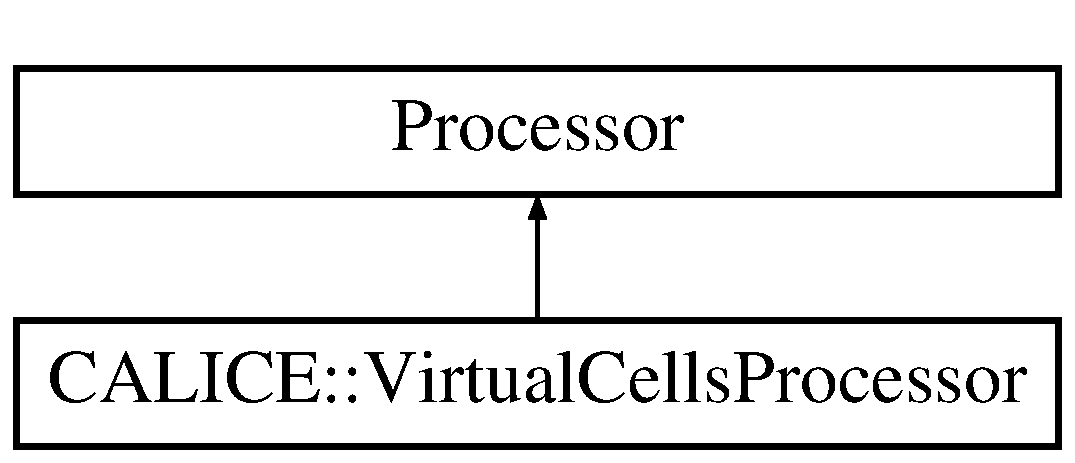
\includegraphics[height=2.000000cm]{classCALICE_1_1VirtualCellsProcessor}
\end{center}
\end{figure}
\subsection*{Public Member Functions}
\begin{DoxyCompactItemize}
\item 
virtual Processor $\ast$ {\bfseries new\-Processor} ()\label{classCALICE_1_1VirtualCellsProcessor_a58e24bc7d4c0f33f9de682678f8f68e0}

\item 
virtual void {\bfseries init} ()\label{classCALICE_1_1VirtualCellsProcessor_abac6131a93b8f735222d63e695d6b401}

\item 
virtual void {\bfseries process\-Event} (L\-C\-Event $\ast$evt)\label{classCALICE_1_1VirtualCellsProcessor_af2bb752abf56392252ff8cd222a99bc4}

\item 
virtual void {\bfseries end} ()\label{classCALICE_1_1VirtualCellsProcessor_a0644fe9c1934cda6f2107eea88faf2ba}

\end{DoxyCompactItemize}
\subsection*{Static Public Member Functions}
\begin{DoxyCompactItemize}
\item 
static Mapped\-Container\\*
$<$ {\bf Virtual\-Cells} $>$ $\ast$ {\bf get\-Virtual\-Cells} (const std\-::string \&processor\-Name)
\end{DoxyCompactItemize}


\subsection{Detailed Description}
Processor that provides virtual cells of $1\mathrm{cm}\times1\mathrm{cm}$

To obtain the object in other processors use\-: \doxyref{Virtual\-Cells\-Processor\-::get\-Virtual\-Cells}{p.}{classCALICE_1_1VirtualCellsProcessor_ab5d72dc70bac4d60c96e3d446e89750f}( \char`\"{}virtual\-Cells processor name\char`\"{} )

\begin{DoxyParagraph}{processor parameters}
\begin{TabularC}{2}
\hline
steering file parameter name &description  \\\cline{1-2}
{\bfseries {\itshape  Mapping\-Processor\-Name }}&name of the mapping processor that provides the necessary Mapper class \\\cline{1-2}
{\bfseries {\itshape  Cell\-Description\-Processor\-Name }}&name of the cell description processor that provides the necessary cell description information \\\cline{1-2}
\end{TabularC}

\end{DoxyParagraph}
\begin{DoxyAuthor}{Author}
{\tt Benjamin.\-Lutz@desy.\-de} 
\end{DoxyAuthor}
\begin{DoxyVersion}{Version}
0.\-1 
\end{DoxyVersion}
\begin{DoxyDate}{Date}
June 2009 
\end{DoxyDate}


\subsection{Member Function Documentation}
\index{C\-A\-L\-I\-C\-E\-::\-Virtual\-Cells\-Processor@{C\-A\-L\-I\-C\-E\-::\-Virtual\-Cells\-Processor}!get\-Virtual\-Cells@{get\-Virtual\-Cells}}
\index{get\-Virtual\-Cells@{get\-Virtual\-Cells}!CALICE::VirtualCellsProcessor@{C\-A\-L\-I\-C\-E\-::\-Virtual\-Cells\-Processor}}
\subsubsection[{get\-Virtual\-Cells}]{\setlength{\rightskip}{0pt plus 5cm}Mapped\-Container$<$ {\bf Virtual\-Cells} $>$ $\ast$ C\-A\-L\-I\-C\-E\-::\-Virtual\-Cells\-Processor\-::get\-Virtual\-Cells (
\begin{DoxyParamCaption}
\item[{const std\-::string \&}]{processor\-Name}
\end{DoxyParamCaption}
)\hspace{0.3cm}{\ttfamily [static]}}\label{classCALICE_1_1VirtualCellsProcessor_ab5d72dc70bac4d60c96e3d446e89750f}
static function to obtain a Mapped\-Container with virtual cells


\begin{DoxyParams}[1]{Parameters}
\mbox{\tt in}  & {\em processor\-Name} & name of the \doxyref{Virtual\-Cells\-Processor}{p.}{classCALICE_1_1VirtualCellsProcessor} that takes care of this \doxyref{Virtual\-Cells}{p.}{classCALICE_1_1VirtualCells}. \\
\hline
\end{DoxyParams}
\begin{DoxyReturn}{Returns}
pointer to the Mapped\-Container including \doxyref{Virtual\-Cells}{p.}{classCALICE_1_1VirtualCells} 
\end{DoxyReturn}


The documentation for this class was generated from the following files\-:\begin{DoxyCompactItemize}
\item 
/nfs/dust/ilc/user/marquezh/\-Calice\-Soft\-\_\-w\-\_\-\-I\-L\-C\-Soft\-\_\-v02-\/03-\/02/calice\-\_\-analysis/addon\-Procs/include/Virtual\-Cells\-Processor.\-hh\item 
/nfs/dust/ilc/user/marquezh/\-Calice\-Soft\-\_\-w\-\_\-\-I\-L\-C\-Soft\-\_\-v02-\/03-\/02/calice\-\_\-analysis/addon\-Procs/src/Virtual\-Cells\-Processor.\-cc\end{DoxyCompactItemize}

%--- End generated contents ---

% Index
\newpage
\phantomsection
\addcontentsline{toc}{part}{Index}
\printindex

\end{document}
